\documentclass[11pt,a4paper]{article}
\usepackage[utf8]{inputenc}
\usepackage[T1]{fontenc}
\usepackage[english]{babel}
\usepackage[margin=2.2cm]{geometry}
\usepackage{amsmath,amssymb,booktabs,longtable,tabularx,array}
\usepackage{enumitem,xcolor,hyperref,xurl,tikz}
\usetikzlibrary{arrows.meta,positioning}
\hypersetup{colorlinks=true,linkcolor=blue!55!black,urlcolor=blue!55!black,
  pdftitle={TerraPulse AI: Project Technical Documentation},
  pdfauthor={TerraPulse AI Team}}
\setlist{leftmargin=*,itemsep=3pt}
\setlength{\parskip}{5pt}
\setlength{\emergencystretch}{1.5em}
\setcounter{tocdepth}{2}
\usepackage{graphicx}
\graphicspath{{fig/}}
\usepackage{caption}
\captionsetup{font=small,labelfont=bf,margin=0.6cm}
\usepackage[skins,breakable]{tcolorbox}
\tcbset{boxrule=0.6pt,arc=2pt,left=6pt,right=6pt,top=4pt,bottom=4pt,fonttitle=\bfseries\small,before skip=8pt,after skip=8pt}
\newtcolorbox{intuicion}{colback=blue!4,colframe=blue!55!black,title={Intuition},breakable}
\newtcolorbox{cuidado}{colback=orange!8,colframe=orange!75!black,title={Caution},breakable}
\newtcolorbox{atencion}{colback=orange!8,colframe=orange!75!black,title={Attention},breakable}
\newtcolorbox{ejemplo}[1][Example]{colback=green!5,colframe=green!45!black,title={#1},breakable}
\newcommand{\figura}[3]{%
  \begin{figure}[htbp]\centering
    \IfFileExists{fig/#1.pdf}{%
      \includegraphics[width=#2\linewidth]{fig/#1.pdf}%
    }{%
      \fbox{\begin{minipage}{#2\linewidth}
        \centering\vspace{2.5cm}
        \textit{Pending figure: \detokenize{#1}}\\
        \small Graphic asset not included in the project.
        \vspace{2.5cm}
      \end{minipage}}%
    }
    \caption{#3}\label{fig:#1}
  \end{figure}%
}


% --- common macros
\newcommand{\src}[1]{\nolinkurl{#1}}
\newcommand{\dd}{\mathrm d}
\newcommand{\unit}[1]{\mathrm{#1}}
\newcommand{\warn}[1]{\par\noindent\colorbox{blue!8}{\parbox{.965\linewidth}{\textbf{Critical reading.} #1}}\par}
% --- Part II macros (radar)
\newcommand{\gz}{\ensuremath{\gamma^{0}}}
\newcommand{\sz}{\ensuremath{\sigma^{0}}}
\newcommand{\por}{\ensuremath{\times}}
\newcommand{\flecha}{\ensuremath{\rightarrow}}
\pdfstringdefDisableCommands{\def\gz{gamma0}\def\sz{sigma0}\def\por{x}\def\flecha{->}\def\src#1{}}

% --- compact \part: no dedicated page
\makeatletter
\renewcommand\part{\if@noskipsec \leavevmode \fi \par \addvspace{4ex}\@afterindentfalse \secdef\@part\@spart}
\def\@part[#1]#2{%
  \refstepcounter{part}%
  \addcontentsline{toc}{part}{\partname~\thepart\hspace{0.6em}#1}%
  {\parindent\z@ \raggedright \interlinepenalty\@M \normalfont
   \Large\bfseries \partname\nobreakspace\thepart \par\nobreak
   \Huge\bfseries #2\markboth{}{}\par}%
  \nobreak \vskip 3ex \@afterheading}
\makeatother

\title{TerraPulse AI\\[4pt]\Large The Changing Pulse of Our Planet\\[6pt]\large Project Technical Documentation\\[2pt]\normalsize Challenge: Dancing with SARs / Earth System Trend Detective}
\author{TerraPulse AI Team}
\date{November 15, 2026}
\begin{document}

\maketitle
\tableofcontents
\listoffigures
\listoftables
\newpage

\part{The Project}
\label{part:proyecto}

\section{Project Summary}
\label{sec:resumen}

TerraPulse AI (``The Changing Pulse of Our Planet'') is an open web platform that turns radar
observations from the NASA--ISRO NISAR mission into understandable and reproducible geospatial evidence.
It is not merely an image viewer. It builds a complete, traceable pipeline: it queries the ASF catalog, verifies that
scenes are comparable (track, frame, polarization, processing version, and maturity), subsets
GCOV products to the Region of Interest (ROI), and computes backscatter change between two dates
($\Delta\sigma^0$ in dB). It then contrasts that change against independent sources such as GPM IMERG
precipitation, HLS optical imagery, or OPERA products.

For the \emph{Dancing with SARs} challenge, the project studies Chiapas, Mexico, using a pair of comparable NISAR
scenes from June to October 2026. Every reported figure can be traced back to the scene, date,
parameters, and code that produced it. The project strictly distinguishes between observation, inference, and prediction, and
does not attribute physical causes that radar alone cannot demonstrate.

This matters because radar observes both day and night and penetrates cloud cover---a critical capability in tropical
regions. Furthermore, it empowers researchers, civil protection authorities, and communities to make decisions backed by verifiable data.

\section{Detailed Description}
\label{sec:detalle}

\subsection{What Does It Do and How Does It Work?}

TerraPulse AI carries public NISAR radar data (L-band) from the original archival file to an interactive
map without losing track of where every single value comes from. The workflow follows five steps:
\begin{enumerate}
  \item \textbf{Catalog.} Queries ASF and groups GCOV products into comparable stacks. To be grouped together, scenes must match in track, frame, flight direction, polarization, processing version (CRID), and maturity level.
  \item \textbf{Comparability control.} Rejects pairs that must never be mixed, such as BETA with
        PROVISIONAL or two different CRIDs.
  \item \textbf{Smart subsetting.} Each full scene weighs approximately 7\,GB. Instead of downloading the entire granule, the system
        streams over HTTPS only the \texttt{.h5} chunks intersecting the Region of Interest.
        It then verifies scene identity, actual spatial coverage (99.6\,\% valid pixels in the
        Chiapas working pair), and pixel-grid identity across both dates.
  \item \textbf{Inspection and web export.} Generates Cloud-Optimized GeoTIFFs (COGs), web map layers, and statistical charts, all accompanied by provenance metadata.
  \item \textbf{Web platform.} Displays SAR layers on an interactive map, a before/after swipe comparator, charts, and quantitative metric panels.
\end{enumerate}
Additionally, the platform includes exploratory physical simulators operating over real NASADEM terrain:
\begin{itemize}
  \item \textbf{Flood simulation:} uses the LISFLOOD-FP hydrodynamic solver with synthetic rainfall scenarios
        (Part~\ref{part:inundacion}).
  \item \textbf{Terrain solar irradiance:} computes solar position and clear-sky direct irradiance
        for a selected ROI and timestamp (Part~\ref{part:solar}).
\end{itemize}
Both are explicitly presented as unvalidated physical models, never as direct observations.

\subsection{Benefits and Impact}

Radar operates at night and sees through clouds---a decisive advantage in Chiapas, where persistent cloud cover limits optical satellites. TerraPulse enables researchers, civil protection agencies, students, and local communities to explore surface changes using verifiable data. It also clearly explains what each metric means and what it does not mean. Because the workflow is open and reproducible, anyone can replicate it in another region.

\subsection{Tools and Technology Stack}

\begin{itemize}
  \item \textbf{Languages:} Python 3.11, TypeScript, SQL.
  \item \textbf{Data Sources:} NISAR GCOV (ASF Vertex / NASA Earthdata) and NASADEM. Auxiliary validation sources include GPM IMERG, HLS, and OPERA.
  \item \textbf{Processing:} h5py, rasterio, GDAL, xarray, rioxarray, geopandas, numpy, asf\_search,
        earthaccess, LISFLOOD-FP, and pvlib.
  \item \textbf{Backend:} Django, GeoDjango, Django REST Framework, PostgreSQL + PostGIS, Celery + Redis.
  \item \textbf{Frontend:} React, Vite, MapLibre GL, Three.js, Chart.js.
  \item \textbf{Infrastructure:} Docker and Docker Compose, with automated testing in pytest.
\end{itemize}

\section{Context: Why Use Radar to Observe Surface Changes?}
\label{sec:contexto}

Repeatedly observing the Earth's surface is the foundation of almost every question regarding environmental change:
how much water covers a floodplain after a storm, how vegetation evolves throughout the year, or whether
soil moisture increased or decreased between two dates. Optical satellites (which produce photograph-like imagery) answer these questions well when skies are clear and daylight is available. In a tropical region like Chiapas, where cloud cover is persistent throughout the rainy season, those conditions are rarely met precisely when observations are most needed.

A Synthetic Aperture Radar (SAR) operates differently. Instead of recording reflected sunlight, the satellite itself emits microwave pulses toward the Earth's surface and measures the returning echo. Consequently:
\begin{itemize}
  \item \textbf{It is independent of daylight:} the radar provides its own illumination, enabling nighttime observation.
  \item \textbf{It penetrates clouds:} at microwave wavelengths, clouds and light rain cause virtually no attenuation.
  \item \textbf{It measures physical properties distinct from color:} the returning signal is governed by surface geometry, roughness, and dielectric constant (moisture), rather than visual appearance.
\end{itemize}
The NISAR mission, jointly developed by NASA and the Indian Space Research Organisation (ISRO), carries both L-band and S-band radars. TerraPulse AI utilizes the \textbf{L-band} (wavelength near 24\,cm), which penetrates vegetation canopies deeper than shorter wavelengths and responds to larger vegetation structures and soil moisture. The platform consumes GCOV (\emph{Geocoded Polarimetric Covariance}) products, which are already orthorectified onto a map projection grid.

\begin{intuicion}
A radar image is \emph{not} a black-and-white photograph. Each pixel measures how much microwave energy returned to the satellite from that ground cell. A dark pixel might be calm water (which specularly reflects the pulse away from the sensor) or a mountain slope facing away from the radar; a bright pixel might be a metal roof, a tree trunk standing in floodwater (double-bounce), or pure statistical fluctuation (\emph{speckle}). Reading a SAR image means understanding which physical mechanism produced each brightness level.
\end{intuicion}

\section{The End-to-End Data Chain}
\label{sec:cadena}

TerraPulse AI is not a standalone utility, but a processing chain in which each link receives verified inputs from the preceding stage and delivers verifiable outputs to the next. Figure~\ref{fig:cadena-datos} summarizes the workflow, and Table~\ref{tab:eslabones} details the inputs, outputs, and verification checks at each stage.

\begin{figure}[htbp]
\centering
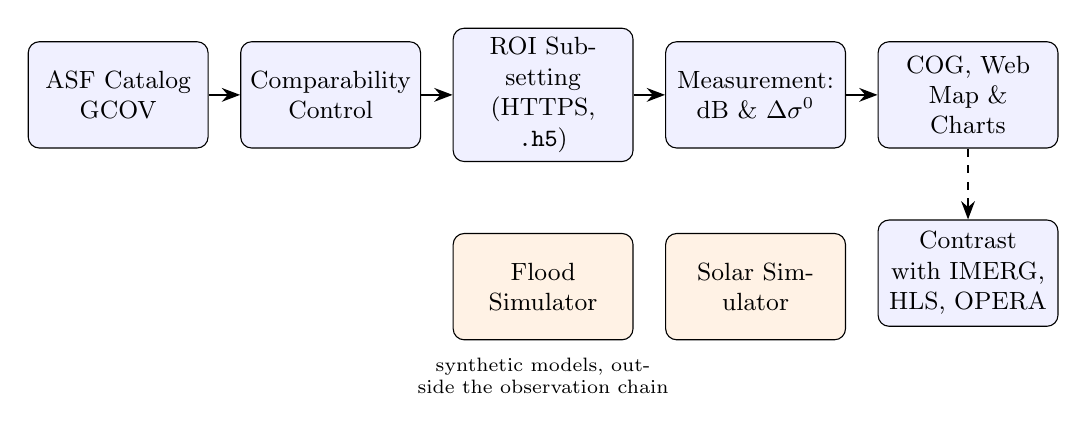
\begin{tikzpicture}[node distance=4mm,
  caja/.style={draw,rounded corners,fill=blue!6,align=center,text width=2.05cm,minimum height=1.35cm,font=\small},
  mod/.style={caja,fill=orange!10},
  fl/.style={-{Stealth},thick}]
\node[caja] (a) {ASF Catalog\\GCOV};
\node[caja,right=of a] (b) {Comparability Control};
\node[caja,right=of b] (c) {ROI Subsetting (HTTPS, \texttt{.h5})};
\node[caja,right=of c] (d) {Measurement: dB \& $\Delta\sigma^0$};
\node[caja,right=of d] (e) {COG, Web Map \& Charts};
\node[mod,below=9mm of c] (f) {Flood Simulator};
\node[mod,right=of f] (g) {Solar Simulator};
\node[caja,below=9mm of e] (h) {Contrast with IMERG, HLS, OPERA};
\draw[fl] (a)--(b); \draw[fl] (b)--(c); \draw[fl] (c)--(d); \draw[fl] (d)--(e);
\draw[fl,dashed] (e)--(h);
\node[font=\scriptsize,below=1mm of f,text width=4.3cm,align=center] {synthetic models, outside the observation chain};
\end{tikzpicture}
\caption{The observation chain (top) and the exploratory simulators (bottom, in orange). The simulators share NASADEM terrain elevation but neither feed into nor validate radar measurements.}
\label{fig:cadena-datos}
\end{figure}

\begin{table}[htbp]
\centering\small
\begin{tabularx}{\linewidth}{p{.19\linewidth}p{.24\linewidth}p{.22\linewidth}X}
\toprule
\textbf{Stage} & \textbf{Input} & \textbf{Output} & \textbf{Verification Check}\\\midrule
Catalog & ASF Query & GCOV product stacks & Metadata matches identical track and frame\\
Comparability & Candidate stacks & Accepted or rejected pairs & Same track, frame, direction, polarization, CRID, and maturity\\
Subsetting & $\approx$7\,GB scene, ROI & ROI data chunks & Scene identity, valid spatial coverage, and identical grid across dates\\
Measurement & Linear power \gz{} \& mask & dB, multilook, $\Delta\sigma^0_{\mathrm{dB}}$ & Valid pixels, common radiometric scale, reproducible statistics\\
Export & Measurement rasters & COG, web layers, charts & Metadata and hashes linking each layer to its source granule\\
Contrast & Change maps & Independent evidence & Consistency with precipitation, optical imagery, and OPERA products\\\bottomrule
\end{tabularx}
\caption{Inputs, outputs, and verification checks across each stage of the observation chain.}
\label{tab:eslabones}
\end{table}

\paragraph{Why Order Matters.} Comparability control occurs \emph{before} spending bandwidth on subsetting and long before computing any difference map. A pair of scenes with different processing versions (CRID) or different maturity levels (e.g., BETA vs.\ PROVISIONAL) can exhibit differences caused by processor calibration changes rather than surface phenomena. Rejecting incompatible pairs upfront is both computationally cheaper and scientifically more honest than trying to explain away a spurious change afterward.

\section{Observation, Inference, and Prediction}
\label{sec:tres-niveles}

One core rule governs the entire project: every statement is labeled according to its epistemic origin. Table~\ref{tab:niveles} summarizes the three levels and how they are treated throughout this document.

\begin{table}[htbp]
\centering\small
\begin{tabularx}{\linewidth}{p{.17\linewidth}p{.36\linewidth}X}
\toprule
\textbf{Level} & \textbf{Definition} & \textbf{Example in This Document}\\\midrule
Observation & A quantity read or computed directly from the product, with full traceability to the source file. &
The mean $\gamma^0_{HH}$ within the ROI is $-8.055$\,dB (Part~\ref{part:radar}).\\
Inference & A plausible physical explanation that has not yet been verified with independent data. &
The 4.3\,dB gap between the linear mean and the dB mean \emph{likely} reflects mixed land cover and strong point scatterers.\\
Prediction / Scenario & Output of a numerical model under explicitly declared assumptions. &
Simulated water depth under synthetic rainfall (Part~\ref{part:inundacion}); clear-sky direct irradiance (Part~\ref{part:solar}).\\\bottomrule
\end{tabularx}
\caption{The three levels of scientific statements and how they are distinguished.}
\label{tab:niveles}
\end{table}

The exploratory simulators always belong to the third level. The fact that the service returns a well-formed, downloadable map with complete metadata proves that the \emph{technical integration} works; it does not prove that the map depicts an observed real-world event. This distinction is deliberately reiterated in Parts~\ref{part:inundacion} and~\ref{part:solar}.

\section{How This Document Is Designed to Be Read}
\label{sec:como-leer}

This document can be read across three complementary layers that coexist in every part:
\begin{enumerate}
  \item \textbf{Intuition.} Blue callout boxes and diagrams that explain, without equations, what a formula does and why it is needed.
  \item \textbf{Equation.} The full mathematical expression with all variables and physical units, accompanied by dimensional analysis where helpful.
  \item \textbf{Example and Code.} Green callout boxes containing step-by-step worked calculations and references to the exact repository functions implementing the method.
\end{enumerate}
Additionally, orange \textbf{Caution} boxes highlight interpretations that might appear intuitive at first glance but are scientifically unjustified. Numerical examples not derived from an actual NISAR granule are explicitly labeled as \emph{illustrative}; figures computed from the Stage 1 working product are identified as such.

\section{Organization of This Document}
\label{sec:organizacion}

This document compiles the complete technical documentation of the project across thirteen parts:
\begin{description}[style=nextline]
  \item[Part~I. The Project.] What TerraPulse AI is, why it uses SAR, how data flows end-to-end, and how observations are separated from model assumptions.
  \item[Part~II. Fundamentals of Synthetic Aperture Radar.] What an imaging radar measures, what speckle is, and what a GCOV product contains. This provides the conceptual foundation for all radar equations.
  \item[Part~III. Radar Equations.] Radiometric measurement, multitemporal change detection, and physical interpretation; which equation produces each Stage 1 figure, with supporting explanations and diagrams.
  \item[Part~IV. From Pixel to Analysis.] The step-by-step journey of a single pixel from raw HDF5 reading to regional statistics, with numerical examples and a pre-interpretation checklist.
  \item[Part~V. DG2 Flood Simulation by Region of Interest.] Conceptual guide, shallow-water equations, DG2 discretization, inputs, verifiable lifecycle, and how to read simulation outputs.
  \item[Part~VI. Terrain Solar Irradiance.] Exact scope of the implemented solar pipeline and conceptual foundations of direct irradiance over complex topography.
  \item[Part~VII (and Part~XI). 3D ROI Terrain Viewer and SAR Geometric Mask.] Client-side 3D topographic mesh construction, Terrarium decoding, adaptive despike filtering, Lambertian shading, and side-looking SAR geometric mask (layover, shadow, and critical slopes).
  \item[Part~VIII. Derivations and Mathematical Proofs.] Step-by-step mathematical proofs supporting previous parts: speckle statistics, radar geometry, shallow-water equations, and solar geometry.
  \item[Part~IX. Worked Exercises and Guided Case Studies.] Numerical problems with complete solutions and physical interpretation covering radar, flood simulation, and solar radiation.
  \item[Part~X. Appendices.] Glossary, consolidated symbol table, unit conversions, frequently asked questions, and quality checklists.
  \item[Part~XII. Seismic Simulator, GMPE Attenuation, P/S Wavefronts, and Signal Processing.] Seismological formulation ($M_0$, $M_w$), regional Mexican GMPEs (Arroyo et al.\ 2010, Garc\'ia et al.\ 2005, crustal), $P/S$ wave kinematics, $50\,\unit{Hz}$ synthetic accelerograms, Arias Intensity, FFT, and STFT spectrograms.
  \item[Part~XIII. Software Architecture, APIs, and Deployment.] Four-layer decoupled architecture, Stage~1 web export and Chart.js rendering, exhaustive REST API contracts, PostGIS/Docker persistence, NASADEM provider, and Solar Simulator API.
\end{description}
Part~\ref{part:radar} describes the radar \emph{observation} chain. Parts~\ref{part:inundacion} and~\ref{part:solar} (along with the 3D Terrain Viewer and Seismic Simulator parts) describe \emph{synthetic or exploratory} models that are never mixed with radar observations and are clearly marked as unvalidated when appropriate.

\noindent\textbf{Note on Notation.} Each part defines its own notation locally rather than enforcing a single global symbol set across distinct physics domains. For instance, in Part~\ref{part:radar} $h$ denotes surface roughness height or ellipsoidal height and $\sigma$ denotes radar cross-section; in Part~\ref{part:inundacion} $h$ denotes water depth above the local bed. Equations and sections are numbered continuously throughout the document; Section~\ref{sec:simbolos-global} compiles the primary symbols.

\clearpage
\part{Fundamentals of Synthetic Aperture Radar}
\label{part:fundamentos}

This part does not introduce project results: instead, it builds the physical vocabulary and intuition that make
the equations in Part~\ref{part:radar} readable. Readers already familiar with SAR may skip ahead; newcomers
to radar imagery will find answers to the questions usually asked in this exact order:
what does the instrument actually measure?, why do radar images look grainy?, and what exactly is inside the
file being downloaded?

\section{What an Imaging Radar Measures}
\label{sec:que-mide}

\subsection{Echo, Delay, and Distance}

A radar emits a microwave pulse and listens for its returning echo. Because the electromagnetic wave travels at the speed of light $c$, the
round-trip travel time $\tau$ determines the distance to the target:
\begin{equation}
  r = \frac{c\,\tau}{2}.
  \label{eq:rango}
\end{equation}
The factor $1/2$ appears because the pulse traverses the path twice (outbound and return). Two targets at different distances
return their echoes at different instants, allowing the radar to sort the scene by distance. This distance measured along the radar line of sight is called \textbf{slant range} and corresponds to $r$ in Figure~\ref{fig:geometria_sar}.

\subsection{Why the Radar Looks Sideways}

If the radar pointed straight down (toward the nadir), two targets located at identical distances on opposite sides of the
satellite ground track would return simultaneous echoes, making it impossible to tell left from right (left/right ambiguity). To eliminate this
ambiguity, SAR sensors are \emph{side-looking}, pointing toward only one side of the flight path. In the Stage 1 working product,
the orbit is ascending (flying northward) and the radar looks to the left---that is, westward. The illuminated ground region forms a long, narrow strip (the \emph{swath}), bounded by a near-range edge and a far-range edge.

\figura{geometria_sar}{0.92}{Acquisition geometry in a cross-track plane perpendicular to the orbit. Slant
range $r$ connects the satellite to the target; $\theta_e$ is the elevation angle at the sensor and $\theta_i$ is the
incidence angle at the target. Drawn over a flat Earth for clarity; Section~\ref{sec:incidencia} accounts for
Earth curvature.}

\subsection{Range Resolution}

The ability to separate two closely spaced targets in the range direction depends on the pulse bandwidth $B$,
not on its pulse duration. Using a frequency-modulated (\emph{chirp}) pulse and pulse compression, the
slant-range resolution is
\begin{equation}
  \delta r = \frac{c}{2B},
  \qquad
  \delta g = \frac{\delta r}{\sin\theta_i},
  \label{eq:res-rango}
\end{equation}
where $\delta g$ is the ground-range resolution projected onto the horizontal surface. As a \emph{generic} example (not NISAR specifications), a bandwidth $B = 20$\,MHz yields $\delta r = 7.5$\,m and, at $\theta_i = 44^\circ$,
$\delta g \approx 10.8$\,m. Notice that $\delta g > \delta r$: projected onto the ground, range resolution degrades at steep
incidence angles and improves further away from the nadir.

\subsection{Azimuth Resolution and Synthetic Aperture}

Along the flight direction (azimuth), a physical antenna of length $D$ illuminates a ground footprint whose width at range
$r$ is approximately $r\lambda/D$. With $\lambda = 0.24$\,m, $D = 10$\,m (illustrative value), and $r \approx
1000$\,km, the raw beam footprint would span about $24$\,km---far too coarse for detailed imaging.

The core idea of \textbf{synthetic aperture} is to exploit the satellite's orbital motion. While a ground target remains
inside the antenna beam, the radar observes it from hundreds of consecutive positions. By coherently combining those echoes (i.e.,
preserving their phase history), the processor achieves the same angular resolution as a virtual antenna whose length equals the distance traveled by the satellite during that observation window. In the ideal \emph{stripmap} mode, the azimuth resolution is
\begin{equation}
  \delta_{az} \approx \frac{D}{2},
  \label{eq:res-az}
\end{equation}
\emph{independent of range}. With $D = 10$\,m, this yields roughly 5\,m, compared to 24\,km for the raw physical beam. That is the fundamental reason SAR exists.

\begin{intuicion}
Range resolution is achieved through \emph{signal bandwidth}. Azimuth resolution is achieved through \emph{platform motion
and phase coherence}. A product with 10\,m pixel spacing, such as the Stage 1 GCOV product, encapsulates both focusing operations plus a subsequent spatial averaging step (multilooking) explained in Section~\ref{sec:speckle}.
\end{intuicion}

\section{L-Band and Polarization}
\label{sec:banda-pol}

\subsection{Wavelength and What the Radar ``Sees''}

An electromagnetic wave interacts strongly with structures of size comparable to its wavelength. The L-band, with
$\lambda \approx 24$\,cm, is \emph{not} sensitive to individual leaves or fine twigs, which are much smaller:
the wave penetrates right through them. Instead, it interacts with tree trunks, primary branches, and the underlying ground surface. Consequently, L-band radar enables studying forest structure and sub-canopy soil moisture---phenomena that shorter wavelengths (C-band, X-band) resolve poorly because they scatter primarily within the upper canopy.

\begin{table}[htbp]
\centering\small
\begin{tabularx}{\linewidth}{p{.12\linewidth}p{.17\linewidth}X}
\toprule
\textbf{Band} & \textbf{Approx.\ $\lambda$} & \textbf{Typical Interaction with Vegetation}\\\midrule
X & 3\,cm & Scattering occurs predominantly at the top of the canopy.\\
C & 5.6\,cm & Limited penetration; interacts with leaves and small branches.\\
L & 24\,cm & Deep canopy penetration; interacts with thick branches, trunks, and ground.\\\bottomrule
\end{tabularx}
\caption{Representative radar wavelengths and their qualitative interaction with vegetation. Values represent
common orders of magnitude rather than specific mission parameters.}
\label{tab:bandas}
\end{table}

\subsection{Polarization: HH and HV}

A radar wave is a transverse electromagnetic wave, meaning its electric field oscillates perpendicular to the direction of propagation. That oscillation orientation is its \textbf{polarization}. A polarimetric radar can transmit and receive using either horizontal (H) or vertical (V) polarization. The two-letter notation indicates transmit and receive polarization; its physical meaning is:
\begin{description}[style=nextline]
  \item[HH] Horizontally transmitted and horizontally received (\emph{co-polarized}). Sensitive
        to surface roughness and double-bounce scattering mechanisms, such as wave reflection between standing water and vertical tree trunks.
  \item[HV] Horizontally transmitted and vertically received (\emph{cross-polarized}). Depolarization is primarily caused by volume scattering from randomly oriented elements such as vegetation canopies. Therefore, HV is typically weaker than HH and strongly sensitive to above-ground woody biomass.
\end{description}

\subsection{Scattering Matrix and Covariance Matrix}

For each resolution cell, the radar measures a complex scattering matrix $\mathbf S$ relating the transmitted electric field to the
received field. Under full H and V transmit/receive, its elements $S_{HH}$, $S_{HV}$, $S_{VH}$, and $S_{VV}$ are
complex numbers (amplitude and phase). In a dual-polarization product containing HH and HV, the GCOV layers \texttt{HHHH} and
\texttt{HVHV} represent the \textbf{linear powers}
\begin{equation}
  \texttt{HHHH} = \langle |S_{HH}|^2 \rangle,
  \qquad
  \texttt{HVHV} = \langle |S_{HV}|^2 \rangle,
  \label{eq:cov-diag}
\end{equation}
which are the diagonal terms of the polarimetric covariance matrix. The angle brackets $\langle\cdot\rangle$
denote spatial averaging across neighboring resolution cells---precisely the multilooking operation described in
Section~\ref{sec:speckle}. Off-diagonal terms (such as $\langle S_{HH}S_{HV}^*\rangle$) store relative phase correlation and are not used in this project.

\begin{cuidado}
\texttt{HHHH} and \texttt{HVHV} store \emph{linear power} (proportional to amplitude squared), not amplitude.
Taking a square root to obtain amplitude or applying $10\log_{10}$ vs.\ $20\log_{10}$ with the wrong convention
will double or halve the resulting decibel values.
\end{cuidado}

\section{Speckle and Multilooking}
\label{sec:speckle}

\subsection{Why a Radar Image Appears Grainy}

Every pixel in a SAR image encompasses numerous elementary scatterers: leaves, pebbles, soil clods, and micro-relief.
The total echo from a resolution cell is the \emph{coherent sum} of their individual contributions,
\begin{equation}
  z = \sum_{k=1}^{M} a_k\, e^{\mathrm{i}\varphi_k},
  \label{eq:fasor}
\end{equation}
where $a_k$ is the amplitude and $\varphi_k$ is the phase of scatterer $k$. Because phase depends on two-way path lengths measured in fractions of a wavelength, $\varphi_k$ varies randomly from one cell to the next. When $M$ is
large, the Central Limit Theorem implies that the real and imaginary components of $z$ are independent Gaussian random variables. From this follow exact and fundamental statistical properties:
\begin{itemize}
  \item The \emph{amplitude} $|z|$ follows a Rayleigh distribution.
  \item The \emph{intensity} (linear power) $P=|z|^2$ follows an exponential distribution with mean $\bar{P}$:
        $p(P)=\bar{P}^{-1}e^{-P/\bar{P}}$.
  \item The standard deviation of $P$ equals its mean: a single-look radar measurement has a 100\,\% relative standard deviation.
\end{itemize}
This produces the characteristic salt-and-pepper graininess known as \textbf{speckle}. Speckle is not instrumental electronic noise: it is a genuine physical consequence of coherent wave interference, and it would persist even in a noise-free radar.

\subsection{Multilooking: Averaging to Reduce Variance}

Averaging $L$ independent intensity samples from a homogeneous surface preserves the expected mean while reducing variance. The average of $L$ independent exponential random variables follows a Gamma distribution:
\begin{equation}
  \bar P_L = \frac{1}{L}\sum_{j=1}^{L}P_j
  \;\sim\; \mathrm{Gamma}\!\left(L,\ \tfrac{\bar{P}}{L}\right),
  \qquad
  \frac{\sigma_{P}}{\bar{P}} = \frac{1}{\sqrt{L}}.
  \label{eq:gamma-ml}
\end{equation}
At $L=1$ the coefficient of variation is 1; at $L=4$ it drops to 0.5; at $L=16$, to 0.25. The trade-off is spatial resolution: averaging $2\times2$ pixels at 10\,m spacing produces a 20\,m pixel. Stage 1 inspection uses $n=2$ for GCOV layers (Equation~\eqref{eq:multilook}), while the change map defaults to $n=5$ (50\,m).

\figura{speckle_imagen}{1.0}{Effect of speckle and multilooking on a \emph{synthetic} test scene (computer-simulated, not a NISAR granule). From left to right: true underlying surface with five backscatter levels; 1-look realization; $2\times2$ multilook average; and $4\times4$ multilook average. All panels are displayed in dB using an identical grayscale stretch.}

\begin{atencion}
\textbf{Nominal Looks vs.\ Equivalent Number of Looks (ENL).} Equation~\eqref{eq:gamma-ml} assumes statistically
\emph{independent} samples. When adjacent pixels are spatially correlated (for instance, due to oversampling during geocoding), the effective number of looks is lower than the number of averaged pixels. The figures in this section therefore represent the theoretical ideal; actual dispersion in a geocoded product can be slightly higher.
\end{atencion}

\subsection{Speckle in Decibels}

Because radiometric analysis is performed in decibels (dB), it is essential to understand how speckle behaves after applying $10\log_{10}$. For a Gamma-distributed variable with $L$ looks and unit linear mean, the expectation and standard deviation in dB are
\begin{equation}
  \mathbb{E}\!\left[10\log_{10}P\right]
  = \frac{10}{\ln 10}\bigl[\psi(L)-\ln L\bigr],
  \qquad
  \operatorname{sd}\!\left[10\log_{10}P\right]
  = \frac{10}{\ln 10}\sqrt{\psi'(L)},
  \label{eq:db-gamma}
\end{equation}
where $\psi$ is the digamma function and $\psi'$ is the trigamma function. For large $L$, $\psi'(L)\approx 1/L$ and the standard deviation approaches $\approx 4.34/\sqrt{L}$\,dB. Table~\ref{tab:speckle-db} lists representative values.

\begin{table}[htbp]
\centering\small
\begin{tabular}{rrr}
\toprule
$L$ & Mean Bias in dB [dB] & Speckle Std.\ Dev.\ [dB]\\\midrule
1  & $-2.51$ & 5.57\\
2  & $-1.17$ & 3.49\\
4  & $-0.57$ & 2.31\\
9  & $-0.25$ & 1.49\\
16 & $-0.14$ & 1.10\\
64 & $-0.03$ & 0.54\\\bottomrule
\end{tabular}
\caption{Theoretical speckle statistics in dB for $L$ independent looks (Equation~\eqref{eq:db-gamma}). The bias is the difference between the mean of the dB values and the dB of the linear mean.}
\label{tab:speckle-db}
\end{table}

\figura{speckle_hist}{1.0}{Speckle probability distributions for $L=1,4,16$. Left: in linear power scale, the exponential distribution ($L=1$) is strongly skewed. Right: in dB scale, distributions become nearly bell-shaped but retain a long left tail toward low dB values. Each curve is computed from 400,000 simulated samples.}

\figura{multilook_teoria}{1.0}{Left: speckle standard deviation in dB as a function of $L$ (exact trigamma curve vs.\ $4.34/\sqrt{L}$ asymptote). Right: Jensen's inequality bias due solely to speckle, starting at 2.51\,dB for $L=1$ and decaying toward zero as $L$ increases.}

\begin{ejemplo}[Jensen's Inequality in a $2\times2$ Block]
Consider a $2\times2$ block with linear power values $0.10$, $0.20$, $0.05$, and $0.15$. Their linear mean is
$0.125$, which converts to $10\log_{10}(0.125)=-9.03$\,dB. Conversely, if each pixel is converted to dB first
($-10.00$, $-6.99$, $-13.01$, $-8.24$) and then averaged, the result is $-9.56$\,dB. The $0.53$\,dB discrepancy
is the logarithmic bias avoided by averaging \emph{in linear power first}, exactly as implemented in Stage 1 and the change detection pipeline.
\end{ejemplo}

\section{From Radar Echo to the GCOV Product}
\label{sec:gcov}

\subsection{Processing Levels}

A SAR satellite does not downlink ready-made map images; it downlinks raw unfocused signal data processed across hierarchical levels:
\begin{enumerate}
  \item \textbf{Level 0 (Raw Data):} unfocused digitized radar echoes.
  \item \textbf{Level 1 (Single Look Complex, SLC):} focused in range and azimuth, retaining complex amplitude and phase per pixel in radar slant-range/azimuth coordinates.
  \item \textbf{Level 2 (Geocoded Products):} orthorectified onto a geographic or UTM map grid and radiometrically calibrated. GCOV stores the geocoded polarimetric covariance matrix; GSLC stores the geocoded complex image.
\end{enumerate}

\subsection{What a GCOV Product Contains}

From the Stage 1 GCOV HDF5 granule, the pipeline consumes the following datasets and metadata grids:
\begin{description}[style=nextline]
  \item[\texttt{HHHH}, \texttt{HVHV}] Linear backscatter power normalized to the $\gamma^0$ convention declared in the product metadata (\texttt{outputBackscatterNormalizationConvention = gamma0}).
  \item[\texttt{mask}] Per-pixel validity byte: 0 denotes invalid data, 255 denotes outside acquisition swath, and positive integers ($1\dots254$) identify valid sub-swaths.
  \item[\texttt{rtcGammaToSigmaFactor}] The pixel-by-pixel geometric factor $F$ that converts $\gamma^0$ into $\sigma^0$ (Equation~\eqref{eq:gamma-sigma}).
  \item[\texttt{radarGrid}] A coarse 3D metadata cube (incidence angle, elevation angle, slant range, line-of-sight unit vectors) sampled at 500\,m horizontal spacing across multiple ellipsoidal height planes.
\end{description}

\subsection{Radiometric Terrain Correction (RTC)}

Pixel brightness depends not only on surface physical properties, but also on the actual ground area illuminated by each range-azimuth resolution cell. A slope tilted toward the radar intercepts a larger radar beam cross-section per ground cell than flat terrain; a slope tilted away intercepts less. \textbf{Radiometric Terrain Correction} (RTC) uses a Digital Elevation Model (DEM) to compute the true illuminated area and normalize backscatter power accordingly. This topographic area normalization is what distinguishes GCOV's $\gamma^0$ from a simple flat-Earth division by $\cos\theta_i$ (Section~\ref{sec:retro}).

\figura{geometria_local}{0.95}{Ellipsoidal incidence vs.\ local topographic incidence. On a radar-facing slope, the local incidence angle is smaller than the ellipsoidal angle (yielding stronger return and, in extreme cases, \emph{layover}); on the opposite slope it is larger and, if it reaches or exceeds $90^\circ$, produces radar shadow. The Stage 1 GCOV product does not apply an automated shadow/layover mask (\texttt{shadowMaskingApplied = False}).}

\subsection{Geometric Distortions: Foreshortening, Layover, and Shadow}

Because a radar sorts returns by \emph{slant distance} rather than horizontal coordinate, topography induces three characteristic geometric distortions:
\begin{itemize}
  \item \textbf{Foreshortening:} slopes facing the radar appear compressed in ground range.
  \item \textbf{Layover:} when a radar-facing slope is steeper than the incidence angle, the mountain peak lies closer to the satellite than its base and is mapped ``folded over'' ahead of the base, mixing echoes from distinct terrain locations.
  \item \textbf{Radar Shadow:} back-slopes steeper than the radar look angle are shielded from direct illumination and return only thermal noise.
\end{itemize}
Because Stage 1 operates over mountainous terrain in Chiapas where these distortions occur and are not pre-masked in the GCOV file, the product mask indicates \emph{where} valid samples exist, while the 3D Terrain Viewer's SAR Geometric Mask (Part~\ref{part:relieve3d}) diagnoses \emph{where} topography compromises radar geometry.

\section{What Radar Measures and What It Does Not}
\label{sec:mide-no-mide}

Summarizing these physical principles in a lookup table helps prevent common misinterpretations.

\begin{table}[htbp]
\centering\small
\begin{tabularx}{\linewidth}{p{.3\linewidth}X}
\toprule
\textbf{Radar responds to\ldots} & \textbf{Radar does \emph{not} respond to\ldots}\\\midrule
Surface roughness at the scale of the radar wavelength & Visual color, surface temperature, or chemical composition alone\\
Dielectric constant, governed primarily by liquid water content & Water depth or the specific physical cause of a change\\
Local slope geometry and orientation relative to line of sight & Subsurface features beneath dense wet soil or deep water\\
Vegetation architecture (trunks, branches, canopy volume) & Plant species identity or photosynthetic health directly\\\bottomrule
\end{tabularx}
\caption{What can and cannot be inferred directly from SAR pixel backscatter.}
\label{tab:mide-no-mide}
\end{table}

This physical asymmetry is why TerraPulse AI insists that $\Delta\gamma^0$ or $\Delta\sigma^0$ measures a change in
\emph{radar backscatter response} rather than identifying, by itself, the underlying physical cause (Section~\ref{sec:cambio}).

\part{Radar Equations: Measurement, Change Detection, and Interpretation}
\label{part:radar}

NISAR's Synthetic Aperture Radar (SAR) does not solve fluid-dynamics equations. Its underlying physics is
electromagnetic (Maxwell's equations, microwave propagation, and scattering). This part
compiles the mathematical formulations operating across the TerraPulse AI radar pipeline: the monostatic radar equation,
backscatter normalization conventions, decibel conversion, and multitemporal change detection between comparable dates. It also
presents the physical scattering models used to \emph{interpret} observed changes, as well as the interferometric phase relation
that would apply only if the selected case study were crustal deformation. Section~\ref{sec:figuras} explains, figure by
figure, which exact equations produce the Stage 1 inspection plots (\path{data/explore/.../figuras/}).

\section{The Radar Equation}
\label{sec:radar}

For a monostatic radar (where the same antenna transmits and receives), the power received from a point scatterer is
\begin{equation}
  P_r = \frac{P_t\, G^2\, \lambda^2\, \sigma}{(4\pi)^3 R^4},
  \label{eq:radar}
\end{equation}
where
\begin{itemize}
  \item $P_t$: transmitted power;
  \item $G$: antenna gain;
  \item $\lambda$: radar wavelength (NISAR L-band, \emph{Frequency A}: $\lambda \approx 24$\,cm);
  \item $R$: slant-range distance between radar and target;
  \item $\sigma$: radar cross-section (RCS) of the target (m$^2$).
\end{itemize}

\subsection{Understanding the Radar Equation}
\label{sec:entender-radar}

Equation~\eqref{eq:radar} is a three-step energy budget, in which each multiplicative factor answers a distinct
physical question:

\begin{enumerate}
  \item \textbf{How much energy reaches the target?} The transmitting antenna focuses power $P_t$ into a directional beam with gain $G$. At distance $R$, that energy spreads over a sphere of surface area $4\pi R^2$, so the incident power flux density is $P_tG/(4\pi R^2)$.
  \item \textbf{How much energy does the target scatter back?} The target intercepts and re-radiates microwave energy as if it had an effective area $\sigma$ (its radar cross-section) directed back toward the sensor. On the return path, that scattered power spreads over a second sphere of area $4\pi R^2$.
  \item \textbf{How much energy does the receiving antenna capture?} The receiving antenna has an effective aperture area $A_e = G\lambda^2/(4\pi)$. Multiplying the returning power flux density by $A_e$ yields the received power $P_r$.
\end{enumerate}
Multiplying the three factors yields $G^2$ (one for transmission, one for reception), $\lambda^2$ from the effective aperture, and $R^4$ in the denominator: an $R^{-2}$ spreading loss outbound and another $R^{-2}$ inbound. That fourth-power range decay is the single most important feature of the radar equation.

\begin{table}[htbp]
\centering\small
\begin{tabular}{lcc}
\toprule
If you double\ldots & $P_r$ changes by & Linear Factor\\\midrule
slant range $R$ & $-12.04$\,dB & $2^{-4}$\\
wavelength $\lambda$ & $+6.02$\,dB & $2^{2}$\\
antenna gain $G$ & $+6.02$\,dB & $2^{2}$\\
radar cross-section $\sigma$ & $+3.01$\,dB & $2^{1}$\\
transmitted power $P_t$ & $+3.01$\,dB & $2^{1}$\\\bottomrule
\end{tabular}
\caption{Sensitivity of received power $P_r$ to each variable in Equation~\eqref{eq:radar} (holding all others constant), computed via $10\log_{10}$ of the ratio.}
\label{tab:sensibilidad-radar}
\end{table}

\begin{ejemplo}[Does Slant-Range Variation Across the Swath Matter?]
Across the Stage 1 Chiapas ROI, slant range varies from 976.8 to 1018.1\,km. Due solely to the $R^{-4}$ spreading factor, the raw echo from an identical surface type would arrive $40\log_{10}(976.8/1018.1)=-0.72$\,dB weaker at the far edge than at the near edge. That \emph{instrumental} gradient is comparable in magnitude to subtle environmental changes. That is why GCOV products are radiometrically calibrated: the delivered backscatter coefficient has already compensated for range spreading, antenna pattern, and processor gains so that two pixels covering identical terrain yield the same $\gamma^0$ regardless of range.
\end{ejemplo}

\paragraph{Why This Equation Is Not Evaluated Directly.} Nowhere in the TerraPulse pipeline do we compute $P_r$: the NISAR L2 processor has already calibrated the raw signal and delivered a normalized backscatter coefficient. The radar equation matters because it explains \emph{what is isolated inside} that coefficient and why geometric normalization is required. The only remaining free physical variable of scientific interest is $\sigma$: how the Earth's surface scatters the incident wave.

\section{Backscatter Coefficients}
\label{sec:retro}

For distributed targets (soil, vegetation canopies, water bodies), radar cross-section $\sigma$ is normalized by a reference area to obtain a dimensionless backscatter coefficient:
\begin{equation}
  \sigma^0 = \frac{\langle \sigma \rangle}{A_{\text{ground}}} .
\end{equation}
The three standard radar conventions differ in which reference plane defines the area. Over flat terrain with local incidence angle $\theta_i$:
\begin{equation}
  \beta^0 = \frac{\sigma^0}{\sin\theta_i},
  \qquad
  \gamma^0 = \frac{\sigma^0}{\cos\theta_i}.
\end{equation}
In NISAR GCOV products, $\gamma^0$ is normalized by the true illuminated area projected onto the plane perpendicular to the radar line of sight, computed rigorously from a Digital Elevation Model (RTC). Because this corrects for topographic slope, over rugged terrain the flat-Earth relation $\gamma^0 = \sigma^0/\cos\theta_i$ is only a first-order approximation.

The GCOV \texttt{HHHH} layer stores the diagonal covariance term $\langle |S_{HH}|^2 \rangle$: the terrain-flattened backscatter power for horizontal transmit and horizontal receive.

\subsection{Intuition: Three Ways to Divide by an Area}
\label{sec:tres-coef}

Total radar cross-section $\sigma$ scales with resolution cell size: a large agricultural parcel scatters more total energy than a small patch of the exact same crop. Comparing intrinsic surface properties requires dividing by a reference area. The only difference among $\sigma^0$, $\beta^0$, and $\gamma^0$ is \emph{which geometric plane} is chosen for that reference area, as summarized in Table~\ref{tab:areas-ref}.

\begin{table}[htbp]
\centering\small
\begin{tabularx}{\linewidth}{p{.1\linewidth}p{.38\linewidth}X}
\toprule
 & \textbf{Reference Area} & \textbf{Flat-Earth Relation}\\\midrule
$\sigma^0$ & Ground surface area, $A_g$ & Baseline definition: $\sigma^0=\langle\sigma\rangle/A_g$\\
$\beta^0$ & Area in the slant-range plane, $A_g\sin\theta_i$ & $\beta^0=\sigma^0/\sin\theta_i$\\
$\gamma^0$ & Area in the plane perpendicular to line of sight, $A_g\cos\theta_i$ &
$\gamma^0=\sigma^0/\cos\theta_i$\\\bottomrule
\end{tabularx}
\caption{The three backscatter conventions and their reference planes. Dividing by a smaller projected area yields a larger numerical coefficient.}
\label{tab:areas-ref}
\end{table}

Why does GCOV default to $\gamma^0$? Over heterogeneous topography and volume-scattering media such as forests, $\gamma^0$ exhibits a much weaker dependence on incidence angle than $\sigma^0$: normalizing by the area perpendicular to the incoming beam removes most of the geometric projection effect. This makes measurements across a swath much more uniform.

\begin{ejemplo}[Comparing the Three Conventions at $\theta_i = 44^\circ$ on Flat Terrain]
Starting from $\sigma^0=-10.00$\,dB:
\begin{itemize}
  \item $\beta^0$ in dB: $-10.00-10\log_{10}(\sin 44^\circ)=-10.00+1.58=-8.42$\,dB.
  \item $\gamma^0$ in dB: $-10.00-10\log_{10}(\cos 44^\circ)=-10.00+1.43=-8.57$\,dB.
\end{itemize}
The three conventions differ by 1.4 to 1.6\,dB---more than enough to create a spurious ``change'' if conventions are mixed. The strict operational rule is never to add, subtract, or compare values across different backscatter conventions.
\end{ejemplo}

\paragraph{What the GCOV Factor $F$ Represents.} Because GCOV normalizes $\gamma^0$ using DEM-derived illuminated area rather than the flat-Earth approximation, the HDF5 file provides a pixel-level conversion layer (\texttt{rtcGammaToSigmaFactor}) to convert $\gamma^0$ into $\sigma^0$ via $\sigma^0=\gamma^0F$. Over flat terrain $F\approx\cos\theta_i$; over slopes it diverges from $\cos\theta_i$. In the Stage 1 Chiapas ROI, converting HH from $\gamma^0$ to $\sigma^0$ shifts the dB mean from $-8.06$ to $-9.79$\,dB (a difference of $-1.73$\,dB), compared to $-1.43$\,dB expected for flat terrain at the mean incidence angle of $43.9^\circ$. The remaining $0.30$\,dB difference reflects actual topographic relief.

\section{Conversion to Decibels}

\begin{equation}
  \sigma^0_{\text{dB}} = 10 \log_{10} \sigma^0 .
  \label{eq:db}
\end{equation}
The exact same transformation applies to $\gamma^0$. When working with complex SLC data (GSLC), linear power is computed first via $10\log_{10}|z|^2$.

\subsection{Why Radar Analysis Uses Decibels}

Linear backscatter values span five to six orders of magnitude: a calm lake may return one-thousandth of the power scattered by a metal roof. In linear units, almost the entire image histogram collapses near zero while a few bright point targets dominate the numerical scale. Applying $10\log_{10}$ achieves three essential goals simultaneously: it compresses the dynamic range into a tractable interval (typically $-30$ to $+10$\,dB), transforms multiplicative ratios into additive differences, and stabilizes speckle variance (which is multiplicative in linear power) into an additive noise term of constant width across all brightness levels.

\figura{escala_db}{1.0}{Left: $10\log_{10}$ compresses six orders of magnitude in linear power into a 60\,dB interval. Right: the inverse mapping from decibels to linear power ratio (highlighting $+3$\,dB $\to 2\times$ and $+10$\,dB $\to 10\times$).}

\begin{table}[htbp]
\centering\small
\begin{tabular}{rrr|rrr}
\toprule
dB & Power Ratio & Meaning & dB & Power Ratio & Meaning\\\midrule
$+1$ & 1.26 & $26\,\%$ increase & $-1$ & 0.79 & $21\,\%$ decrease\\
$+3$ & 2.00 & double power & $-3$ & 0.50 & half power\\
$+6$ & 3.98 & nearly quadruple & $-6$ & 0.25 & one quarter\\
$+10$ & 10 & tenfold & $-10$ & 0.10 & one tenth\\
$+20$ & 100 & hundredfold & $-20$ & 0.01 & one hundredth\\\bottomrule
\end{tabular}
\caption{Decibel-to-linear power ratio equivalences. Every $+3$\,dB doubles linear power; every $+10$\,dB multiplies power by 10.}
\label{tab:db-razon}
\end{table}

\paragraph{Common Pitfalls.}
\begin{itemize}
  \item \textbf{Averaging decibels directly.} While dB summary statistics describe the log-transformed histogram, physical spatial averaging (multilooking) must be performed in linear power prior to taking $10\log_{10}$ (Equation~\eqref{eq:multilook} and Jensen's inequality).
  \item \textbf{Using $20\log_{10}$ instead of $10\log_{10}$.} Power quantities require $10\log_{10}$; amplitude quantities require $20\log_{10}$ (since $10\log_{10}(|z|^2) = 20\log_{10}|z|$).
  \item \textbf{Taking the logarithm of zero or negative numbers.} Invalid or masked pixels ($\le 0$) must never be mapped to $-\infty$\,dB; the pipeline masks them as $\mathrm{NaN}$.
  \item \textbf{Adding decibels as if they were linear powers.} Combining two equal signals of $-10$\,dB does not yield $-20$\,dB or $0$\,dB: their linear powers add ($0.1+0.1=0.2$), yielding $10\log_{10}(0.2) \approx -7$\,dB.
\end{itemize}

\section{Change Detection Between Two Comparable Dates}
\label{sec:cambio}

This section documents the mathematical and computational change detection pipeline between two comparable NISAR GCOV acquisitions (Frequency~A, L-band), implemented in \src{pipeline/preprocess.py}, \src{pipeline/change.py}, and \src{pipeline/roi_explore.py}, as well as its real-time interactive recalculation web service (\texttt{POST /api/roi-jobs/\{id\}/change} and \src{web/src/components/ChangeControls.tsx}).

Before any pixel-by-pixel comparison is allowed, candidate scenes must pass strict comparability verification (\src{pipeline/compat.py}): they must match in product type (\texttt{GCOV}), orbital track, frame, flight direction (\texttt{ASCENDING} or \texttt{DESCENDING}), polarization (\texttt{HH}, \texttt{HV}), spatial posting ($10\times 10\,\unit{m}$), Composite Release ID (\texttt{CRID}), and data maturity (\texttt{PROVISIONAL} or \texttt{VALIDATED}, never mixing with \texttt{BETA}). Furthermore, both ROI subsets must share the exact same cartographic UTM grid (identical CRS, affine transform, and array dimensions); the pipeline \textbf{never resamples} one scene to force alignment with another.

\subsection{Preprocessing and Linear-Power $n\times n$ Multilook Filtering}
\label{subsec:cambio-multilook}

Before computing temporal differences, each scene undergoes three preprocessing steps in \src{pipeline/preprocess.py}:
\begin{enumerate}
  \item \textbf{Product Validity and ROI Polygon Masking:} any pixel whose product \texttt{mask} equals $0$ (invalid) or $255$ (outside swath), or whose pixel center falls outside the ROI polygon reprojected into the product's native UTM CRS (e.g., \texttt{EPSG:32615} in Chiapas), is set to $\mathrm{NaN}$.
  \item \textbf{RTC Radiometric Quantity Selection:} by default, the pipeline uses terrain-flattened backscatter $\gz$ in linear power. Optionally, via CLI flags, $\sz = \gz \cdot F$ can be selected using the GCOV \texttt{rtcGammaToSigmaFactor} layer $F$.
  \item \textbf{Speckle Reduction via $n\times n$ Linear-Power Multilooking:}
        to suppress coherent speckle variance prior to differencing, the linear power array $P_t(i,j) \equiv \gz_t(i,j)$ at epoch $t \in \{t_1, t_2\}$ is partitioned into disjoint $n\times n$ pixel blocks $B_{I,J}$ starting from the top-left corner (discarding remainder rows or columns along the bottom/right edges). Let $V_{I,J} = \{(i,j) \in B_{I,J} : P_t(i,j) \text{ is finite and } P_t(i,j) > 0\}$ denote the subset of valid pixels inside block $(I,J)$. The multilooked linear power is:
        \begin{equation}
          \bar{P}_t(I,J) =
          \begin{cases}
            \displaystyle\frac{1}{|V_{I,J}|} \sum_{(i,j)\in V_{I,J}} P_t(i,j), & \text{if } |V_{I,J}| \ge f_{\min}\,n^2, \\[10pt]
            \mathrm{NaN}, & \text{if } |V_{I,J}| < f_{\min}\,n^2,
          \end{cases}
          \label{eq:cambio-multilook-lineal}
        \end{equation}
        where the minimum valid block coverage fraction is fixed at $f_{\min} = 0.5$ (\texttt{min\_valid\_fraction = 0.5}).
\end{enumerate}

Given native GCOV pixel dimensions $\Delta x = \Delta y = 10\,\unit{m}$, the change pipeline defaults to $n = 5$ ($5\times 5$ blocks), yielding an output grid with effective spatial resolution and pixel area:
\begin{equation}
  \Delta x_{\mathrm{ML}} = n \cdot \Delta x = 5 \times 10\,\unit{m} = 50\,\unit{m}, \qquad
  A_{\mathrm{pixel}} = |a_{\mathrm{ML}} \cdot e_{\mathrm{ML}}| = 50\,\unit{m} \times 50\,\unit{m} = 0.0025\,\unit{km^2}.
  \label{eq:cambio-res-50m}
\end{equation}
In the web UI, users can switch dynamically among $n \in \{2, 5, 10\}$, corresponding to effective resolutions of $20\,\unit{m}$, $50\,\unit{m}$ (default), and $100\,\unit{m}$.

\begin{cuidado}
\warn{Multilook filtering must always be computed on linear power $\gz$ prior to logarithmic conversion.}
Averaging values already converted to decibels computes the geometric mean of linear powers ($\frac{1}{N}\sum 10\log_{10} P_k = 10\log_{10}(\prod P_k)^{1/N}$), which by Jensen's inequality introduces a systematic negative bias ($\approx -2.5\,\unit{dB}$ at $L=1$) and distorts inter-date ratios. For this reason, \src{pipeline/roi_explore.py} persists the masked linear-power GeoTIFFs (\path{layers/<granuleId>/geotiff/gamma0_<capa>.tif}) on disk and performs all dynamic resolution recalculations directly from linear power.
\end{cuidado}

\subsection{Logarithmic Backscatter Difference ($\Delta\gz_{\mathrm{dB}}$)}
\label{subsec:cambio-delta-db}

Once the multilooked linear power fields $\bar{P}_t(I,J)$ are obtained for both dates on the identical $n\Delta x$ grid, each date is converted to decibels:
\begin{equation}
  \gz_{\mathrm{dB},t}(I,J) =
  \begin{cases}
    10\log_{10}\!\bigl(\bar{P}_t(I,J)\bigr), & \text{if } \bar{P}_t(I,J) > 0, \\
    \mathrm{NaN}, & \text{otherwise.}
  \end{cases}
  \label{eq:cambio-a-db}
\end{equation}

For two comparable acquisitions at reference epoch $t_1$ and target epoch $t_2$, the temporal backscatter difference (\texttt{delta\_db} in \src{pipeline/change.py}) is defined cell-by-cell as:
\begin{equation}
  \Delta\gz_{\mathrm{dB}}(I,J) = \gz_{\mathrm{dB},t_2}(I,J) - \gz_{\mathrm{dB},t_1}(I,J)
  = 10\log_{10}\!\left(\frac{\bar{P}_{t_2}(I,J)}{\bar{P}_{t_1}(I,J)}\right).
  \label{eq:delta}
\end{equation}
If a cell $(I,J)$ is $\mathrm{NaN}$ at either $t_1$ or $t_2$, $\Delta\gz_{\mathrm{dB}}(I,J)$ propagates as $\mathrm{NaN}$. The exact same expression holds for $\sz$ ($\Delta\sz_{\mathrm{dB}} = \sz_{\mathrm{dB},t_2} - \sz_{\mathrm{dB},t_1}$) because the geometric conversion factor $F(I,J)$ cancels out under identical orbital viewing geometry.

\subsection{Physical Meaning of $\Delta\gz_{\mathrm{dB}}$}

Equation~\eqref{eq:delta} shows that a difference in decibels measures ten times the base-10 logarithm of the power ratio between $t_2$ and $t_1$. Referring to Table~\ref{tab:db-razon}: a change of $\Delta\gz_{\mathrm{dB}} = +3\,\unit{dB}$ means the ground cell returned \textbf{twice as much microwave power} at $t_2$ ($\bar{P}_{t_2}/\bar{P}_{t_1} \approx 2$), whereas $\Delta\gz_{\mathrm{dB}} = -3\,\unit{dB}$ indicates that backscattered power dropped by \textbf{half} ($\bar{P}_{t_2}/\bar{P}_{t_1} \approx 0.5$).
In the platform's visual outputs (COG and Web Mercator PNG in \texttt{EPSG:3857}), $\Delta\gz_{\mathrm{dB}}$ is rendered using a fixed diverging blue--white--red colormap clamped to $[-6, +6]\,\unit{dB}$: blue denotes backscatter decrease ($\Delta < 0$), white denotes stability ($\Delta \approx 0$), and red denotes backscatter increase ($\Delta > 0$).

\begin{figure}[htbp]
\centering
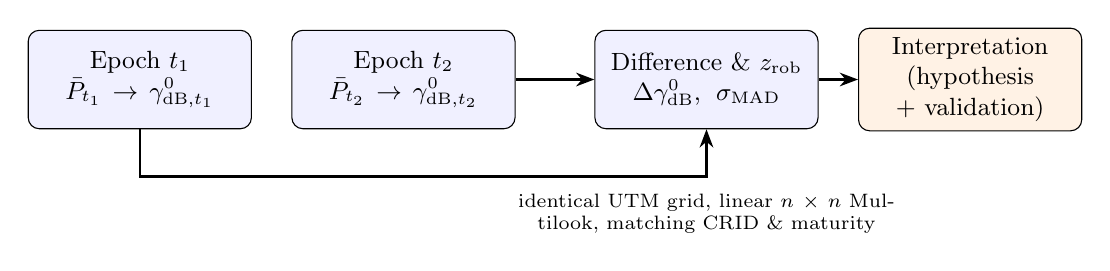
\begin{tikzpicture}[node distance=5mm,
  caja/.style={draw,rounded corners,fill=blue!6,align=center,text width=2.6cm,minimum height=1.25cm,font=\small},
  fl/.style={-{Stealth},thick}]
\node[caja] (a) {Epoch $t_1$\\$\bar{P}_{t_1} \to \gz_{\mathrm{dB},t_1}$};
\node[caja,right=of a] (b) {Epoch $t_2$\\$\bar{P}_{t_2} \to \gz_{\mathrm{dB},t_2}$};
\node[caja,right=10mm of b] (c) {Difference \& $z_{\mathrm{rob}}$\\$\Delta\gz_{\mathrm{dB}},\; \sigma_{\mathrm{MAD}}$};
\node[caja,right=of c,fill=orange!10] (d) {Interpretation\\(hypothesis + validation)};
\draw[fl] (b)--(c); \draw[fl] (a.south) |- ++(0,-6mm) -| (c.south);
\draw[fl] (c)--(d);
\node[font=\scriptsize,below=7mm of c,text width=6.2cm,align=center] {identical UTM grid, linear $n\times n$ Multilook, matching CRID \& maturity};
\end{tikzpicture}
\caption{Change detection workflow in TerraPulse AI: Multilooking is applied in linear power to each comparable epoch prior to dB differencing and robust MAD standardization. Physical interpretation remains strictly separate from radiometric measurement.}
\label{fig:flujo-delta}
\end{figure}

\begin{figure}[htbp]
  \centering
  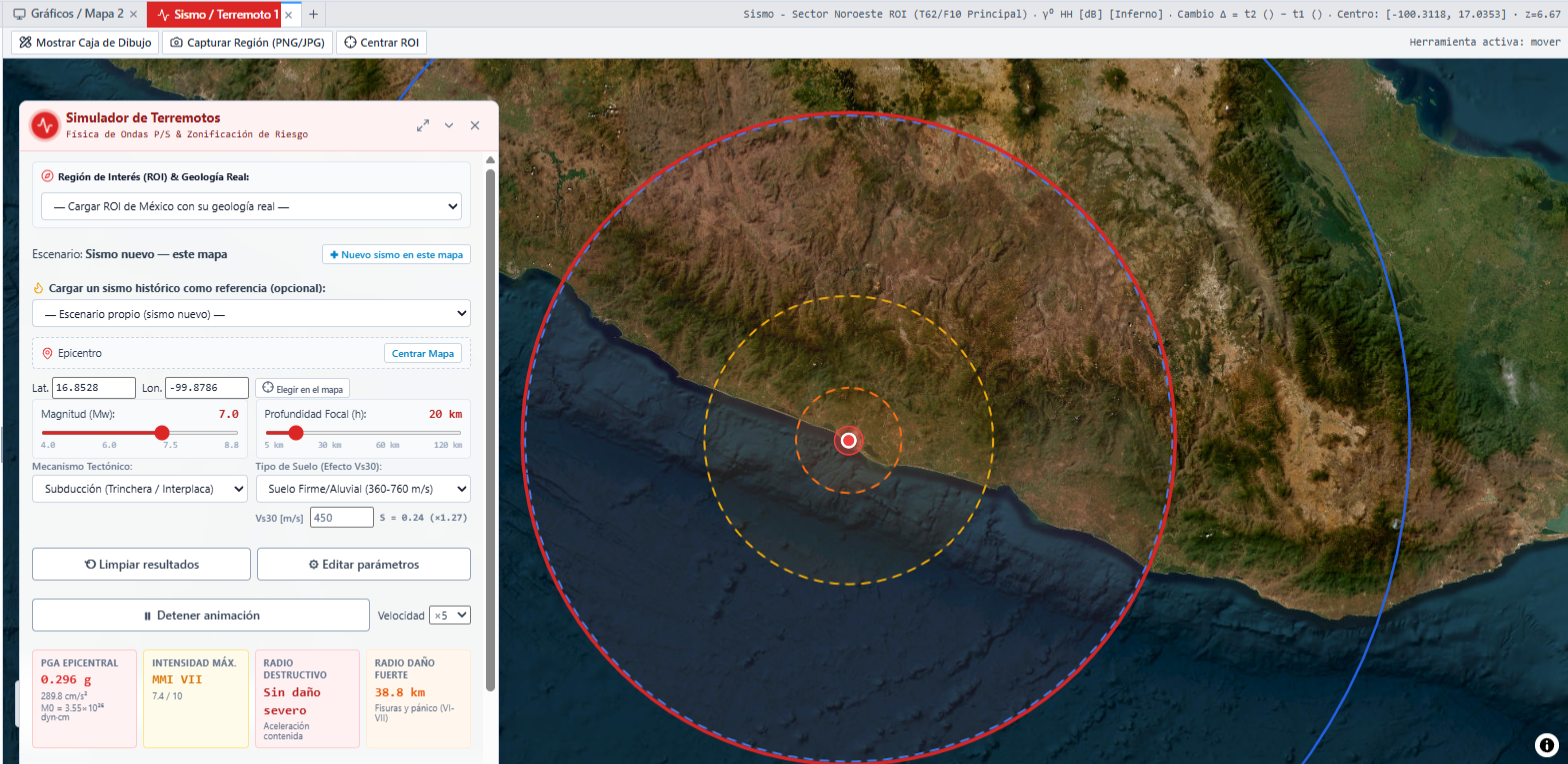
\includegraphics[width=0.84\textwidth]{fig/IMG_cambio_sar_mapa_delta.png}
  \caption{Visualization of the $\Delta\gz_{\mathrm{dB}}$ change map in the TerraPulse AI web interface (\textbf{Change $\Delta$} mode) over an active ROI in Chiapas. The diverging blue--white--red palette ($-6\,\unit{dB}$ to $+6\,\unit{dB}$) maps spatial areas where backscatter decreased (blue), remained stable (white), or increased (red) between $t_1$ and $t_2$.}
  \label{fig:cambio-sar-mapa-web}
\end{figure}

\subsection{Three Reasons Two Dates May Differ and the Effect of Speckle}

\begin{description}[style=nextline]
  \item[Genuine physical surface change.] Variations in soil dielectric moisture, flooding or drying of water bodies, canopy structural changes, agricultural tillage, or land-cover disturbance. This is the target signal.
  \item[Acquisition or processor mismatch.] Different viewing geometry, track, frame, processor version (\texttt{CRID}), or calibration maturity. The strict comparability gate in \src{pipeline/compat.py} eliminates this error source by design.
  \item[Residual statistical fluctuation (\emph{speckle}).] Residual speckle after multilooking is statistically independent between $t_1$ and $t_2$, producing a non-zero difference distribution even over completely unchanged terrain.
\end{description}

If each single-date dB image has a speckle standard deviation $\sigma_L$ (Equation~\eqref{eq:db-gamma}) and the two acquisitions are independent, the theoretical standard deviation of the difference $\Delta\gz_{\mathrm{dB}}$ in the absence of real change is:
\begin{equation}
  \sigma_{\Delta} = \sqrt{2}\,\sigma_L .
  \label{eq:sigma-delta}
\end{equation}
For $L=1$, $\sigma_{\Delta} \approx 7.9\,\unit{dB}$; for $L=4$, $\approx 3.3\,\unit{dB}$; and for $L=16$, $\approx 1.6\,\unit{dB}$ (Figure~\ref{fig:delta_distribucion}). Consequently, a single unaveraged pixel changing by $+3\,\unit{dB}$ between two dates proves \emph{nothing}: it lies well within random speckle fluctuation.

\figura{delta_distribucion}{0.78}{Theoretical probability distribution of $\Delta\sigma^0_{\mathrm{dB}}$ when \emph{no} true ground change has occurred---only independent speckle at each date---for $L=1,4,16$ equivalent looks (400,000 simulated pairs).}

When averaging over a block or region containing $N_{\mathrm{ind}}$ independent samples, the difference standard deviation decreases as $1/\sqrt{N_{\mathrm{ind}}}$:
\begin{equation}
  \sigma_{\Delta,\mathrm{region}} \approx \frac{\sqrt{2}\,\sigma_L}{\sqrt{N_{\mathrm{ind}}}} .
  \label{eq:sigma-region}
\end{equation}
Because adjacent 10\,m pixels in a geocoded GCOV product exhibit spatial correlation, the effective number of independent samples $N_{\mathrm{ind}}$ inside an $n\times n$ window is smaller than $n^2$. Therefore, rather than relying on an idealized theoretical formula, TerraPulse AI \textbf{empirically measures} the background noise floor directly from each ROI's $\Delta\gz_{\mathrm{dB}}$ distribution using robust statistics.

\subsection{Standardized Anomaly: Robust $z$-Score via MAD}
\label{subsec:cambio-zscore-mad}

To quantify how unusual each cell's backscatter change is relative to the background variability of its own Region of Interest, \src{pipeline/change.py} (\texttt{robust\_zscore}) computes a robust $z$-score based on the spatial median and the \textbf{Median Absolute Deviation (MAD)}.

Let $\Omega$ denote the set of all valid (finite) cells in the difference map $\Delta(I,J) \equiv \Delta\gz_{\mathrm{dB}}(I,J)$ within the ROI. First, the spatial median change is computed:
\begin{equation}
  m_{\Delta} = \operatorname{median}_{(I,J)\in\Omega}\!\bigl(\Delta(I,J)\bigr).
  \label{eq:cambio-mediana}
\end{equation}
Next, the median absolute deviation from $m_{\Delta}$ is evaluated and scaled by the Gaussian consistency factor $k = 1 / \Phi^{-1}(0.75) \approx 1.4826$ (\texttt{MAD\_TO\_SIGMA = 1.4826}):
\begin{equation}
  \mathrm{MAD} = \operatorname{median}_{(I,J)\in\Omega}\!\Bigl(\bigl|\Delta(I,J) - m_{\Delta}\bigr|\Bigr),
  \qquad
  \sigma_{\mathrm{MAD}} = 1.4826 \cdot \mathrm{MAD}.
  \label{eq:cambio-mad-sigma}
\end{equation}
Using this robust scale estimator $\sigma_{\mathrm{MAD}}$ (recorded in output manifests as \texttt{mad\_robusto\_dB} and \texttt{ruido\_dB}), the standardized anomaly or robust $z$-score for each cell is defined as:
\begin{equation}
  z_{\mathrm{rob}}(I,J) = \frac{\Delta\gz_{\mathrm{dB}}(I,J) - m_{\Delta}}{1.4826\,\mathrm{MAD}}
  = \frac{\Delta\gz_{\mathrm{dB}}(I,J) - m_{\Delta}}{\sigma_{\mathrm{MAD}}}.
  \label{eq:cambio-z-robusto}
\end{equation}
In the degenerate case where all valid pixels are identical ($\sigma_{\mathrm{MAD}} = 0$), the function assigns $z_{\mathrm{rob}}(I,J) = 0$ across all valid cells to prevent division by zero. The resulting field is exported as a 32-bit floating-point GeoTIFF (\path{zscore_<pol>.tif}) and summarized by the percentage of ROI area exceeding three robust standard deviations ($|z_{\mathrm{rob}}| > 3$, field \texttt{pct\_abs\_z\_mayor\_3}).

\begin{intuicion}
\textbf{Why use the median and MAD ($1.4826\,\mathrm{MAD}$) instead of the classical mean $\mu$ and standard deviation $s$?}
If a localized flood or agricultural burn strongly alters $5\,\text{\%}$ of the pixels in an ROI by $+8\,\unit{dB}$ or $-10\,\unit{dB}$, those changed pixels pull the arithmetic mean $\mu$ and artificially inflate the classical standard deviation $s$, masking the anomaly itself (an effect known as \emph{outlier self-masking}). By contrast, the median and MAD have a $50\,\text{\%}$ breakdown point: they ignore the extreme tails where genuine change occurred and measure exclusively the background dispersion of the stable majority of the ROI. The factor $1.4826$ ensures that if the background noise is normally distributed $\mathcal{N}(\mu, \sigma^2)$, $\sigma_{\mathrm{MAD}}$ converges to the true standard deviation $\sigma$.
\end{intuicion}

\subsection{Threshold Classification Rule and Automated Noise-Floor Warning}
\label{subsec:cambio-clasificacion-ruido}

Given a fixed decibel detection threshold $\tau_{\mathrm{dB}} > 0$ (defaulting to $\tau_{\mathrm{dB}} = 3.0\,\unit{dB}$, user-selectable in the web UI across $\{1.5, 2.0, 2.5, 3.0, 4.0, 5.0, 6.0\}\,\unit{dB}$), the \texttt{classify} function in \src{pipeline/change.py} partitions the grid into three discrete classes stored in a signed 8-bit integer GeoTIFF (\path{cambio_<pol>.tif}, with $\text{NoData} = -128$):
\begin{equation}
  C(I,J) =
  \begin{cases}
    -1, & \text{if } \Delta\gz_{\mathrm{dB}}(I,J) \le -\tau_{\mathrm{dB}} \quad\text{(decrease $\ge \tau_{\mathrm{dB}}$)}, \\[4pt]
    \phantom{-}0, & \text{if } \bigl|\Delta\gz_{\mathrm{dB}}(I,J)\bigr| < \tau_{\mathrm{dB}} \quad\text{(stable within threshold)}, \\[4pt]
    +1, & \text{if } \Delta\gz_{\mathrm{dB}}(I,J) \ge +\tau_{\mathrm{dB}} \quad\text{(increase $\ge \tau_{\mathrm{dB}}$)}, \\[4pt]
    -128, & \text{if } \Delta\gz_{\mathrm{dB}}(I,J) \text{ is } \mathrm{NaN} \quad\text{(no data / outside ROI)}.
  \end{cases}
  \label{eq:cambio-clases}
\end{equation}

Over all valid cells $\Omega$, the pipeline computes the physical area and percentage belonging to each class:
\begin{equation}
  A_{c} = N_{c} \cdot A_{\mathrm{pixel}}, \qquad
  P_{c} = 100 \cdot \frac{N_{c}}{|\Omega|}, \qquad
  N_{c} = \bigl|\{(I,J)\in\Omega : C(I,J) = c\}\bigr|, \quad c \in \{-1, 0, +1\}.
  \label{eq:cambio-areas}
\end{equation}

\paragraph{Fixed-dB Threshold Design with ROI Noise-Floor Verification.}
Keeping the classification threshold $\tau_{\mathrm{dB}}$ fixed in decibels (rather than thresholding directly on $|z_{\mathrm{rob}}| > 3$) provides a crucial scientific advantage: a $\pm 3\,\unit{dB}$ change always represents the exact same physical backscatter ratio (doubling or halving of returned power) across any region or epoch, making affected area figures ($\unit{km^2}$) directly comparable across different ROIs. However, a fixed $3\,\unit{dB}$ threshold may be well above the noise floor at $5\times 5$ multilooking yet dangerously close to the speckle noise floor at $2\times 2$ multilooking.

To resolve this without sacrificing cross-ROI radiometric comparability, \src{pipeline/change.py} evaluates on every run the threshold-to-noise ratio against the ROI's empirical noise floor $\sigma_{\mathrm{MAD}}$ (\texttt{NOISE\_FACTOR = 3.0}):
\begin{equation}
  R_{\tau/\text{noise}} = \frac{\tau_{\mathrm{dB}}}{\sigma_{\mathrm{MAD}}},
  \qquad
  \text{Noise Warning} =
  \begin{cases}
    \texttt{True}, & \text{if } \tau_{\mathrm{dB}} < 3\,\sigma_{\mathrm{MAD}} \iff R_{\tau/\text{noise}} < 3.0, \\
    \texttt{False}, & \text{if } \tau_{\mathrm{dB}} \ge 3\,\sigma_{\mathrm{MAD}} \iff R_{\tau/\text{noise}} \ge 3.0.
  \end{cases}
  \label{eq:cambio-regla-aviso-ruido}
\end{equation}
Whenever $\tau_{\mathrm{dB}} < 3\,\sigma_{\mathrm{MAD}}$ (\texttt{umbral\_cerca\_del\_ruido = true}), the backend automatically injects a traceable warning into \path{change.json} and \src{web/src/components/ChangeControls.tsx} displays a prominent UI alert warning that the chosen threshold is less than $3\times$ the ROI's measured noise floor and that a significant fraction of the flagged area may be random speckle (recommending switching to $50$ or $100\,\unit{m}$ resolution or raising $\tau_{\mathrm{dB}}$).

\begin{figure}[htbp]
  \centering
  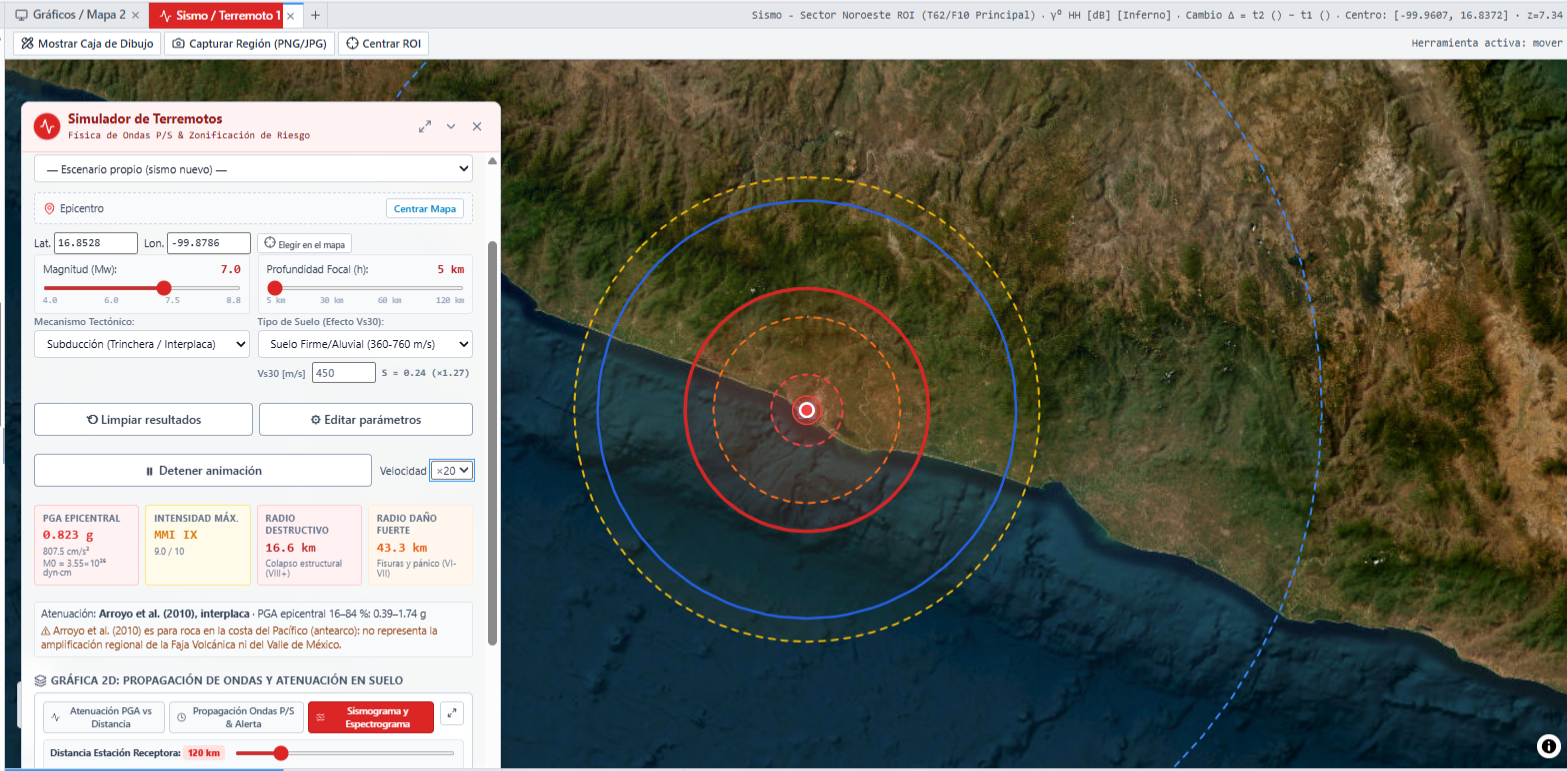
\includegraphics[width=0.82\textwidth]{fig/IMG_cambio_sar_controles_histograma.png}
  \caption{Sidebar change-map controls and telemetry panel (\src{ChangeControls.tsx}) alongside ROI statistics. Displays areas decreasing ($\downarrow$) or increasing ($\uparrow$) beyond $\tau_{\mathrm{dB}}$, median shift $m_{\Delta}$, interactive Multilook resolution ($20/50/100\,\unit{m}$) and threshold ($\pm 1.5$ to $\pm 6\,\unit{dB}$) selectors, empirical noise floor $\sigma_{\mathrm{MAD}}$, ratio $\tau_{\mathrm{dB}}/\sigma_{\mathrm{MAD}}$, percentage of pixels with $|z_{\mathrm{rob}}|>3$, and the automated warning when $\tau_{\mathrm{dB}} < 3\,\sigma_{\mathrm{MAD}}$.}
  \label{fig:cambio-sar-controles}
\end{figure}

\subsection{Dynamic Per-ROI Recalculation Architecture (\texttt{POST /api/roi-jobs/\{id\}/change})}
\label{subsec:cambio-api-recalculo}

Change detection operates both via CLI for the regional Chiapas case study (\texttt{python -m pipeline.change}) and on-demand for any user-drawn ROI in the web platform:
\begin{enumerate}
  \item \textbf{Initial computation during ROI preparation:} once \src{pipeline/roi_explore.py} finishes streaming a comparable GCOV pair over HTTPS, it saves the masked native-resolution ($10\,\unit{m}$) linear power $\gz$ rasters to \path{layers/<granuleId>/geotiff/gamma0_<capa>.tif} and invokes \texttt{build\_change} with default parameters ($n=5 \Rightarrow 50\,\unit{m}$, $\tau_{\mathrm{dB}} = 3.0\,\unit{dB}$).
  \item \textbf{Hot recalculation without re-downloading:} when a user changes resolution ($n \in \{2, 5, 10\}$) or threshold ($\tau_{\mathrm{dB}} \in \{1.5, 2, 2.5, 3, 4, 5, 6\}\,\unit{dB}$) in the UI, the frontend sends \texttt{POST /api/roi-jobs/\{id\}/change} with \texttt{\{"multilook": n, "umbral\_dB": u\}}. The server executes \texttt{recompute\_change} directly from the cached linear-power GeoTIFFs on disk, generating the new Multilook, $\Delta\gz_{\mathrm{dB}}$, $z_{\mathrm{rob}}$, classification raster, and PNG overlay in \textbf{0.1 to 1.5 seconds} without contacting ASF again.
  \item \textbf{Transactional disk cache:} each parameter combination is stored under \path{layers/cambio/ml<n>_u<umbral>/} guarded by an atomic lock directory (\path{<combo>.lock}, with a 5-minute stale-lock timeout) to prevent race conditions. The server permanently retains the default combination (\texttt{ml5\_u3}) plus the 4 most recently requested combinations (\texttt{CHANGE\_CACHE\_KEEP = 4}).
\end{enumerate}

\begin{ejemplo}[Real Results in Chiapas and Noise-Floor Filtering Demonstration in Tuxtla Guti\'errez]
The change pipeline was verified across two spatial scales using real NISAR GCOV products from Track~62, Frame~10, Ascending orbit (\texttt{DHDH}, HH and HV polarizations):

\medskip
\noindent\textbf{1. Regional Chiapas Case Study (\texttt{P05023 PROVISIONAL}, 2026-06-18 $\to$ 2026-10-16, 120-day baseline):}
Over a valid ROI area of $1,469.2\,\unit{km^2}$ processed at $5\times 5$ Multilook ($50\,\unit{m}$) and threshold $\tau_{\mathrm{dB}} = \pm 3.0\,\unit{dB}$:
\begin{itemize}
  \item \textbf{HH Polarization:} median $m_{\Delta} = +0.21\,\unit{dB}$, robust noise $\sigma_{\mathrm{MAD}} = 0.91\,\unit{dB}$ ($R_{\tau/\text{noise}} = 3.3 \ge 3.0$, no noise warning). Area decreasing ($\le -3\,\unit{dB}$) is $6.73\,\unit{km^2}$ ($0.46\,\text{\%}$), while area increasing ($\ge +3\,\unit{dB}$) reaches $27.34\,\unit{km^2}$ ($1.86\,\text{\%}$), with $97.68\,\text{\%}$ stable and $2.71\,\text{\%}$ exceeding $|z_{\mathrm{rob}}| > 3$.
  \item \textbf{HV Polarization:} median $m_{\Delta} = +0.24\,\unit{dB}$, robust noise $\sigma_{\mathrm{MAD}} = 0.91\,\unit{dB}$ ($R_{\tau/\text{noise}} = 3.3$). Area decreasing is $3.33\,\unit{km^2}$ ($0.23\,\text{\%}$) and area increasing is $32.83\,\unit{km^2}$ ($2.24\,\text{\%}$). The pronounced positive asymmetry ($4\times$ more area increasing in HH and $10\times$ in HV) demonstrates that the observed shift cannot be explained by symmetric random speckle, although separating seasonal vegetation growth from soil moisture requires auxiliary validation data.
\end{itemize}

\noindent\textbf{2. $9.3\,\unit{km^2}$ ROI near Tuxtla Guti\'errez (\texttt{P05036 VALIDATED}, 2026-10-28 $\to$ 2026-11-09, 12-day baseline, HH):}
\begin{center}
\small
\begin{tabular}{lcccc}
\toprule
\textbf{Resolution (Multilook)} & \textbf{Noise $\sigma_{\mathrm{MAD}}$} & \textbf{Ratio $\tau_{\mathrm{dB}}/\sigma_{\mathrm{MAD}}$} & \textbf{Down / Up ($\ge 3\,\unit{dB}$)} & \textbf{Warning ($\tau_{\mathrm{dB}} < 3\sigma_{\mathrm{MAD}}$)} \\
\midrule
$20\,\unit{m}$ ($2\times 2$)   & $1.53\,\unit{dB}$ & $2.0\times$ & $2.96\,\text{\%} \;/\; 2.88\,\text{\%}$ & \textbf{Yes (warning triggered)} \\
$50\,\unit{m}$ ($5\times 5$)   & $0.70\,\unit{dB}$ & $4.3\times$ & $0.00\,\text{\%} \;/\; 0.03\,\text{\%}$ & No (reliable) \\
$100\,\unit{m}$ ($10\times 10$) & $0.39\,\unit{dB}$ & $7.7\times$ & $0.00\,\text{\%} \;/\; 0.00\,\text{\%}$ & No (reliable) \\
\bottomrule
\end{tabular}
\end{center}
At $20\,\unit{m}$ resolution over a quiet 12-day interval without extreme weather, nearly $3\,\text{\%}$ of the ROI is falsely flagged in each direction with near-perfect symmetry ($2.96\,\text{\%}$ down vs.\ $2.88\,\text{\%}$ up): the classic signature of unaveraged \emph{speckle}, automatically caught by the condition $R_{\tau/\text{noise}} = 2.0 < 3.0$. Switching to the default $50\,\unit{m}$ ($5\times 5$) resolution cuts the noise floor in half ($0.70\,\unit{dB}$), raises the ratio to $4.3\times$, and eliminates the false positives ($0.00\,\text{\%} / 0.03\,\text{\%}$).
\end{ejemplo}

\begin{atencion}
A high value of $\Delta\gz_{\mathrm{dB}}$ or $|z_{\mathrm{rob}}|$ \textbf{is not a direct detection of flooding, deforestation, or structural damage}. It is a traceable, quantitative measurement of change in L-band radar backscatter that, when combined with terrain geometric masking and independent validation sources (GPM IMERG precipitation, HLS/Sentinel-2 optical imagery, or OPERA products), \emph{can} support a physical hypothesis. Maintaining an explicit boundary between radiometric observation and causal inference is a non-negotiable principle of TerraPulse AI.
\end{atencion}

\section{Scattering Models (For Interpretation, Not Direct Measurement)}

\subsection{Three Mechanisms, Three Signatures}
\label{sec:modelos}

The models in this section serve to reason about \emph{what physical mechanism might be driving} an observed backscatter change. It is useful to keep in mind the three primary ways microwaves interact with natural surfaces (Figure~\ref{fig:mecanismos}):
\begin{description}[style=nextline]
  \item[Specular reflection (smooth surface).] When a surface is smooth relative to the radar wavelength, incident energy reflects away like a mirror, returning almost nothing to the sensor so the pixel appears dark.
  \item[Diffuse or volume scattering.] Over rough soil or inside a vegetation canopy, microwave energy scatters in multiple directions and a moderate fraction returns toward the radar.
  \item[Double-bounce scattering.] Two mutually perpendicular surfaces (calm water and a vertical tree trunk, or ground and a building wall) act as a dihedral corner reflector that directs a strong echo straight back along the incident line of sight.
\end{description}

\figura{mecanismos}{1.0}{The three fundamental backscatter mechanisms. In each panel, the blue arrow represents the incident microwave pulse and the red arrows represent energy scattered back toward the radar.}

\begin{table}[htbp]
\centering\small
\begin{tabularx}{\linewidth}{p{.26\linewidth}p{.3\linewidth}X}
\toprule
\textbf{Surface or Scenario} & \textbf{Dominant Mechanism} & \textbf{Expected Qualitative Response}\\\midrule
Calm open water & Specular reflection & Very low HH and HV (dark).\\
Wind-roughened water or waves & Increased surface roughness & Higher return than calm water; can be confused with land.\\
Dry bare soil $\to$ wet bare soil & Increased dielectric constant & Backscatter increases, especially in HH.\\
Dense forest canopy & Volume scattering & Relatively high HV; reduced sensitivity to underlying soil.\\
Flooded vegetation & Trunk--water double bounce & Strong HH increase; opposite to open-water flooding.\\
Urban / built-up area & Dihedral double bounce & Extremely bright in HH.\\\bottomrule
\end{tabularx}
\caption{Typical qualitative SAR backscatter trends. Actual magnitudes depend on site geometry, incidence angle, and season; this table is a physical guide rather than an automated classification rule.}
\label{tab:escenarios}
\end{table}

\subsection{Surface Roughness: The Rayleigh Criterion}
\label{sec:rayleigh}
A surface behaves as electromagnetically smooth (specular reflection, negligible backscatter) when its root-mean-square height variation $h$ satisfies
\begin{equation}
  h < \frac{\lambda}{8\cos\theta_i}.
\end{equation}
Calm open water satisfies this inequality and appears dark in SAR imagery. Rough or moist soil returns stronger backscatter.

\paragraph{How to Read the Criterion.} The Rayleigh criterion compares the characteristic vertical height of surface irregularities $h$ against a fraction of the radar wavelength projected along the incidence angle. The physical basis is phase difference: if two adjacent points on a surface differ in height by $h$, rays reflected from them differ in two-way path length by $2h\cos\theta_i$. When that path difference is small compared to a quarter wavelength ($\lambda/4$, which yields the factor $\lambda/8$), reflected waves interfere constructively in the specular direction and the surface acts like a mirror; when $h$ exceeds that threshold, phase coherence breaks down and energy scatters diffusely.

\figura{rayleigh}{0.62}{Critical Rayleigh roughness height in L-band as a function of incidence angle $\theta_i$. For $\lambda=24$\,cm at $\theta_i=44^\circ$, the threshold is $4.2$\,cm: surfaces smoother than $4.2$\,cm act specularly; rougher surfaces scatter diffusely.}

For L-band ($\lambda\approx24$\,cm), the critical roughness threshold is $3.5$\,cm at $30^\circ$, $4.2$\,cm at $44^\circ$, and $6.0$\,cm at $60^\circ$. A practical consequence is that wind waves or capillary ripples several centimeters high on a lake can violate the smoothness criterion even in L-band, causing rough water to appear brighter than calm water. Moreover, the exact same ground surface can appear electromagnetically smooth in L-band ($\lambda\approx24$\,cm) yet rough in X-band ($\lambda\approx3$\,cm).

\subsection{Volume Scattering: The Water Cloud Model}
Despite its name, the \emph{water cloud model} is not a hydrodynamic fluid model. Introduced by Attema and Ulaby (1978), it represents a vegetation canopy as a uniform cloud of water-bearing scatterers above a rough soil surface:
\begin{align}
  \sigma^0 &= A\, V_1 \cos\theta_i \left(1 - T^2\right) + T^2\, \sigma^0_{\text{soil}}, \\
  T^2 &= \exp\!\left(-\frac{2 B\, V_2}{\cos\theta_i}\right),
\end{align}
where $V_1$ and $V_2$ are canopy descriptors (e.g., vegetation water content or leaf area index), $A$ and $B$ are empirical coefficients calibrated against field measurements, and $T^2$ is the two-way canopy transmissivity.

\paragraph{How to Read the Model.} The water cloud model is a two-term radiative balance. The first term, $AV_1\cos\theta_i(1-T^2)$, represents direct volume backscatter from the vegetation canopy itself; it grows with canopy density $V_1$ and saturates as $(1-T^2)$ approaches 1. The second term, $T^2\sigma^0_{\text{soil}}$, is the underlying soil backscatter attenuated along its two-way trip through the canopy, decaying exponentially as $V_2$ increases. Figure~\ref{fig:water_cloud} illustrates this balance using \emph{illustrative} parameters: over sparse vegetation, the soil term dominates; over dense canopy, the vegetation volume term dominates.

\figura{water_cloud}{0.66}{Canopy volume and attenuated soil contributions to total $\sigma^0$ in the water cloud model. Parameters $A$, $B$, and $\sigma^0_{\text{soil}}$ are illustrative values chosen to show curve behavior rather than field-calibrated constants.}

\begin{intuicion}
The key physical takeaway from the water cloud model is that \emph{radar sensitivity to soil moisture decreases as vegetation density increases}. A change in soil moisture produces a clear backscatter jump over bare or sparsely vegetated fields, but becomes progressively masked beneath dense forest canopy. Consequently, an identical $\Delta\sigma^0$ value does not imply the same ground condition across different land-cover types.
\end{intuicion}

\subsection{Double-Bounce Scattering}
Standing water beneath trees or marsh plants (flooded vegetation) forms a dihedral corner reflector between the horizontal water surface and vertical trunks or stems, \emph{strongly increasing} backscatter---particularly in co-polarized HH. This response is the exact opposite of open-water flooding (which darkens the image) and is essential when interpreting wetlands or forested floodplains.

\section{Interferometry (Applicable Only to Surface Deformation)}

In Repeat-Pass SAR Interferometry (InSAR), the phase difference $\Delta\phi$ between two complex acquisitions relates to line-of-sight (LOS) surface displacement $\Delta R$ via:
\begin{equation}
  \Delta\phi = \frac{4\pi}{\lambda}\, \Delta R .
\end{equation}
The sign convention depends on the unwrapped interferogram product (GUNW). InSAR measures displacement projected along the radar line of sight, not pure vertical uplift or subsidence.

\subsection{Order of Magnitude for InSAR Displacement}

The relation $\Delta\phi=4\pi\Delta R/\lambda$ implies that one full phase cycle ($2\pi$ radians, or one interferometric \emph{fringe}) corresponds to a line-of-sight displacement of $\Delta R=\lambda/2$. In L-band ($\lambda\approx24$\,cm), each fringe equals $\approx12$\,cm of LOS displacement. While InSAR can resolve fractional-fringe displacements down to centimeters or millimeters, it requires phase coherence to be preserved between acquisitions. TerraPulse AI's GCOV change pipeline operates on radiometric power rather than interferometric phase; this equation is included solely to clarify which physical questions require GUNW phase vs.\ GCOV power.

\section{Equations Behind the Stage 1 Inspection Figures}
\label{sec:figuras}

The Stage 1 reference figures reside in
\path{data/explore/NISAR_L2_PR_GCOV_034_062_A_010_4005_DHDH_A_20261028T114006_20261028T114041_P05036_N_F_J_001/figuras/}.
They correspond to the single-date GCOV T62/F10 ASCENDING granule acquired on 2026-10-28 (CRID \texttt{P05036}) inspected during Stage 1. They are generated by \path{python -m pipeline.etapa1} via functions in \path{pipeline/etapa1_figuras.py}, backed by array readers in \path{pipeline/nisar_h5.py} and \path{pipeline/etapa1.py}.

\paragraph{Traceability.} All numerical values reported in this section are taken directly from \path{metadatos.json} in that exploration directory (generated on 2026-11-13, \texttt{version\_codigo = 98f7e07-dirty}). The \texttt{-dirty} suffix records that uncommitted working-tree edits existed at generation time; for formal citation, the directory can be regenerated from a clean Git commit.

\paragraph{Core Rule.} PNG figures are strictly for \emph{visual inspection}. No quantitative metric is ever computed from 8-bit PNGs (\texttt{AGENTS.md} §5): all statistics are computed from the native \texttt{.h5} floating-point arrays and persisted in \path{metadatos.json} and \path{control/*.csv}.

\subsection{Common Processing Steps Across All Figures}

\paragraph{Native Product Power.} In NISAR GCOV files, the \texttt{HHHH} and \texttt{HVHV} datasets already store linear backscatter power normalized to the convention declared in the HDF5 metadata (\path{rtc/outputBackscatterNormalizationConvention = gamma0}). The reader applies no hidden scaling:
\begin{equation}
  \gamma^0_{pq}(x,y) = \texttt{layer}_{pqpq}(x,y), \qquad pq \in \{\text{HH}, \text{HV}\}.
\end{equation}

\paragraph{Converting \gz{} to \sz.} Using the product's pixel-level \path{rtcGammaToSigmaFactor} layer ($F$):
\begin{equation}
  \sigma^0(x,y) = \gamma^0(x,y)\, F(x,y).
  \label{eq:gamma-sigma}
\end{equation}
Over flat terrain, Section~\ref{sec:retro} implies $F \approx \cos\theta_i$. Because the GCOV processor computes $F$ from the DEM facet geometry, over mountainous relief $F$ departs from $\cos\theta_i$.

\paragraph{Valid Pixel Rule.} A pixel enters quantitative analysis if and only if its product \texttt{mask} is neither 0 (invalid) nor 255 (outside swath) and its coordinate falls inside the ROI polygon:
\begin{equation}
  \text{valid}(x,y) \iff \texttt{mask}(x,y) \notin \{0, 255\} \;\wedge\; (x,y) \in \text{ROI}.
\end{equation}
All other pixels are masked to $\mathrm{NaN}$.

\paragraph{Decibel Conversion.} Equation~\eqref{eq:db} is applied. Whenever $X \le 0$ or $X$ is $\mathrm{NaN}$, the output is set to $\mathrm{NaN}$ (avoiding $-\infty$).

\paragraph{$n\times n$ Multilooking.} Averaging is performed in \emph{linear power} prior to dB conversion. For an $n\times n$ pixel block $B$ containing $N_v$ valid pixels:
\begin{equation}
  \bar{P}_B = \frac{1}{N_v}\sum_{k \in B,\ \text{valid}} P_k,
  \qquad
  \bar{P}_{B,\text{dB}} = 10\log_{10}\bar{P}_B,
  \qquad
  \bar{P}_B = \mathrm{NaN}\text{ if } N_v < 0.5\,n^2 .
  \label{eq:multilook}
\end{equation}
\textbf{Physical Justification:} SAR speckle is multiplicative in linear power. Averaging linear powers reduces variance unbiasedly, whereas averaging decibels introduces a systematic negative Jensen bias (demonstrated in Figure~C). In Stage 1 single-scene inspection, $n = 2$ for GCOV.

\subsection{\texttt{A\_vista\_general\_HHHH.png}: Full-Scene Overview}

\textbf{What It Shows:} Linear \gz{} HH across the entire GCOV scene footprint ($33,480\times 34,128$ pixels at 10\,m posting), with the Chiapas ROI boundary overlaid in red. Blue indicates NoData outside the swath. Function: \path{overview()}.

\textbf{Decimation.} Every $s = 50$-th pixel is sampled along rows and columns without averaging (each plotted sample represents a 500\,m stride):
\begin{equation}
  v_{ij} = \gamma^0_{\text{HH}}(s\,i,\ s\,j).
\end{equation}
Because this is pure decimation rather than block averaging, full single-pixel speckle variability is preserved.

\textbf{Color Normalization (\texttt{PowerNorm}).} Using the 5th and 95th percentiles of the decimated array ($p_b$ and $p_a$) and display gamma exponent $\gamma_v = 0.5$:
\begin{equation}
  t = \left[\operatorname{clip}\!\left(\frac{v - p_b}{p_a - p_b},\, 0,\, 1\right)\right]^{\gamma_v},
\end{equation}
where $t\in[0,1]$ is the grayscale tone (0 black, 1 white). Colorbar tick marks are evenly spaced in display tone $t$, so their corresponding physical values follow
\begin{equation}
  v(t) = p_b + (p_a - p_b)\, t^{1/\gamma_v}, \qquad t = 0,\ 0.2,\ \ldots,\ 1 .
\end{equation}

\textbf{Values in This Figure:} $p_b = 0.0306$, $p_a = 0.5458$; tick marks at $0.031$, $0.051$, $0.113$, $0.216$, $0.360$, and $0.546$. Verification:
$v(0.2) = 0.0306 + 0.5152\cdot 0.2^{2} = 0.0512$.

\textbf{Rationale:} Choosing $\gamma_v < 1$ stretches dark tones so low-backscatter features remain visible in linear units. Note that display exponent $\gamma_v$ is purely a visualization transfer curve and is unrelated to radiometric $\gamma^0$.

\paragraph{How to Read the PowerNorm Transfer Curve.} With $\gamma_v=0.5$, the mapping from linear backscatter $v$ to grayscale tone $t$ is a square-root curve that expands the lower end of the dynamic range. Figure~\ref{fig:powernorm} compares this square-root mapping against a linear stretch and marks the six colorbar tick values ($0.031$ to $0.546$), which are equidistant in display tone $t$ rather than in linear power $v$.

\figura{powernorm}{0.62}{Mapping between linear $\gamma^0_{HH}$ value $v$ and grayscale tone $t$ in Figure~A. Colorbar ticks are evenly spaced in $t$, not in $v$.}

\figura{escalas_pixel}{1.0}{Spatial scale relationships across Stage 1 figures. The native GCOV grid has 10\,m pixels; Figures~B and B2 apply $2\times2$ linear block averaging (20\,m pixels); Figure~A decimates 1 out of every 50 pixels without averaging (500\,m stride).}

\subsection{\texttt{B\_roi\_gamma0\_dB.png}: ROI Backscatter in dB (\gz)}

\textbf{What It Shows:} \gz{} HH and HV inside the ROI bounding window, in dB after $2\times2$ linear multilooking (20\,m pixel spacing). Function: \path{roi_db()}.

\textbf{Equations:} Linear multilook~\eqref{eq:multilook} with $n = 2$, followed by decibel conversion~\eqref{eq:db}.

\textbf{Shared Color Scale.} Both polarizations are rendered using the exact same dB colorbar limits---the 2nd and 98th percentiles of the \emph{combined} HH and HV dB distributions---so brightness levels are directly comparable across panels. In this figure: $-19.36$ to $-3.10$\,dB.

\textbf{Physical Reading:} HV appears systematically darker than HH because cross-polarized volume backscatter is weaker than co-polarized surface/canopy return. Across the ROI, the mean of the dB values is $-8.06$\,dB in HH and $-13.50$\,dB in HV (see Figure~C table).

\paragraph{Step-by-Step Multilooking.} Figure~\ref{fig:multilook_bloques} illustrates how $2\times2$ pixel blocks are aggregated and how missing data are handled. Equation~\eqref{eq:multilook} requires at least $0.5\,n^2=2$ valid pixels per block; otherwise, the output cell is set to $\mathrm{NaN}$.

\figura{multilook_bloques}{0.52}{Illustrative linear-power values across a $4\times4$ pixel array. The four $2\times2$ blocks contain 4, 2, 4, and 1 valid pixels, respectively.}

\begin{table}[htbp]
\centering\small
\begin{tabular}{cccc}
\toprule
Block & Valid Pixels $N_v$ & Linear Mean & Output in dB\\\midrule
Top-left & 4 & 0.125 & $-9.03$\\
Top-right & 2 & 0.275 & $-5.61$\\
Bottom-left & 4 & 0.130 & $-8.86$\\
Bottom-right & 1 & (discarded) & NaN\\\bottomrule
\end{tabular}
\caption{Multilook output for the illustrative array in Figure~\ref{fig:multilook_bloques}. The bottom-right block has $N_v=1<2$ and is masked to $\mathrm{NaN}$.}
\label{tab:bloques}
\end{table}

\paragraph{Why a Shared Color Scale Matters.} By locking both HH and HV to the joint 2nd--98th percentile range, visual tone differences reflect true radiometric differences: HV looks darker because its physical power is lower, not because its histogram was stretched differently.

\subsection{\texttt{B2\_roi\_sigma0\_dB.png}: ROI Backscatter in dB (\sz)}

\textbf{What It Shows:} Identical to Figure~B, except converting to \sz{} via Equation~\eqref{eq:gamma-sigma} prior to multilooking. Shared color scale: $-20.91$ to $-4.54$\,dB.

\textbf{Relation to Figure~B:} In decibels, multiplying by $F$ becomes an addition:
\begin{equation}
  \sigma^0_{\text{dB}} = \gamma^0_{\text{dB}} + 10\log_{10} F .
\end{equation}
\textbf{Order-of-Magnitude Verification:} Across the ROI, the mean dB value for HH shifts from $-8.06$\,dB (\gz) to $-9.79$\,dB (\sz), a difference of $-1.73$\,dB. At the ROI's mean incidence angle (Figure~E, $43.9^\circ$), flat terrain would yield $10\log_{10}\cos 43.9^\circ \approx -1.43$\,dB. The values agree to first order, with the remaining $0.30$\,dB attributable to topographic relief included in $F$.

\subsection{\texttt{C\_histogramas\_gamma0\_dB.png}: Full-Resolution \gz{} Histograms in dB}

\textbf{What It Shows:} The empirical probability distribution of \gz{} in dB at \emph{full native product resolution} (10\,m, no additional multilooking), evaluated across all valid pixels inside the ROI ($n = 14,699,442$ valid pixels per polarization). Function: \path{histograms()}; statistics: \path{power_stats()}.

\textbf{Histogram Binning.} Bins of width $0.1$\,dB spanning $-60$ to $+30$\,dB. The vertical axis reports the percentage of valid ROI pixels falling in each bin:
\begin{equation}
  h_k = 100\,\frac{\#\{\,i : \gamma^0_{\text{dB},i} \in [a_k, a_k + 0.1)\,\}}{n}\ \mathrm{\%}.
\end{equation}
For visual clarity, the horizontal plot axis is clipped to the 0.2nd and 99.8th cumulative percentiles.

\textbf{Vertical Markers and Shaded Band.} Denoting linear power by $P_i$ and decibel value by $D_i = 10\log_{10}P_i$:
\begin{align}
  \text{mean of dB} &= \frac{1}{n}\sum_i D_i, \\
  \text{dB of linear mean} &= 10\log_{10}\!\left(\frac{1}{n}\sum_i P_i\right), \\
  \text{median} &= \operatorname{median}(D_i), \qquad \text{blue shaded band} = [\,p_5(D),\ p_{95}(D)\,].
\end{align}

\textbf{Mathematical Basis: Jensen's Inequality.} Because the logarithm is a strictly concave function,
\begin{equation}
  \frac{1}{n}\sum_i 10\log_{10}P_i \;\le\; 10\log_{10}\!\left(\frac{1}{n}\sum_i P_i\right).
\end{equation}
Consequently, the dashed line (dB of the linear mean) always lies to the right of the solid line (mean of the dB values). As a theoretical benchmark, if $P$ followed a pure single-look exponential distribution over a homogeneous surface, the gap would equal $10\log_{10}(e)\cdot\gamma_E \approx 2.51$\,dB, where $\gamma_E \approx 0.5772$ is the Euler--Mascheroni constant. Multilooking over a homogeneous surface reduces this gap; spatial heterogeneity across mixed land cover increases it.

\textbf{Measured Values in This Figure:}

\begin{longtable}{lrr}
\toprule
 & \textbf{HH} & \textbf{HV} \\
\midrule
Mean of dB & $-8.055$ & $-13.503$ \\
Median (dB) & $-7.880$ & $-13.173$ \\
dB of linear mean & $-3.786$ & $-9.226$ \\
Jensen gap (dB of linear mean $-$ mean of dB) & $4.27$ & $4.28$ \\
$p_5$ to $p_{95}$ interval (dB) & $-14.07$ to $-2.85$ & $-20.00$ to $-8.11$ \\
Standard deviation (dB) & $3.59$ & $3.73$ \\
\bottomrule
\end{longtable}

\textbf{Interpretation (Inference, Not Direct Measurement):} The observed Jensen gap ($\approx 4.3$\,dB) exceeds the pure single-look speckle gap ($2.51$\,dB). This is expected because the Chiapas ROI combines diverse land covers (forests, valleys, urban Tuxtla Guti\'errez, and water) and contains strong point scatterers that pull the linear mean upward (the full-scene HH linear maximum is $7,418$ according to the HDF5 attributes). Determining the exact partition between residual speckle and scene heterogeneity requires segmented land-cover analysis.

\paragraph{A Thought Experiment with Gaussian dB Histograms.} To contextualize the observed $4.27$\,dB gap between the dB of the linear mean and the mean of the dB values, we can compare it against three theoretical benchmarks:
\begin{enumerate}
  \item If the dB values followed a pure \emph{Gaussian} distribution $\mathcal{N}(\mu, s^2)$ (so linear power were log-normal), the exact Jensen gap would be
        \begin{equation}
          \Delta_J = \frac{\ln 10}{20}\,s^2 \approx 0.1151\,s^2 ,
          \label{eq:jensen-gauss}
        \end{equation}
        which for $s=3.59$\,dB yields $1.48$\,dB.
  \item For homogeneous single-look exponential speckle ($L=1$), the gap is $2.51$\,dB.
  \item The observed ROI gap is $4.27$\,dB in HH and $4.28$\,dB in HV---larger than both benchmarks.
\end{enumerate}

\figura{jensen_gauss}{0.64}{Gaussian dB reference benchmark. A Gaussian curve with the observed HH mean and standard deviation ($-8.055$ and $3.59$\,dB) would place the dB of the linear mean at $-6.57$\,dB, far to the left of the actual observed value ($-3.786$\,dB).}

This comparison reveals a key structural feature of the empirical histogram: its upper (bright) tail is heavier than a Gaussian tail in dB, pulling the linear mean rightward. This aligns with our physical inference: a heterogeneous region containing bright urban and topographic reflectors.

\begin{ejemplo}[A Lower Bound on the Effective Number of Looks]
The observed dB standard deviation of HH across the entire ROI is $3.59$\,dB. Pure single-look speckle over a completely uniform target would produce $5.57$\,dB---already \emph{larger} than the total dispersion observed across the heterogeneous ROI. Solving $4.34\sqrt{\psi'(L)}=3.59$ yields $L\approx1.9$. Because real scene texture also contributes positive variance, the product's effective number of looks at 10\,m posting must be at least on the order of $L \ge 2$.
\end{ejemplo}

\subsection{\texttt{D\_mascara.png}: Product Validity Mask}

\textbf{What It Shows:} The spatial distribution of the GCOV \texttt{mask} layer across the rectangular ROI bounding window. Function: \path{mask_map()}.

\begin{longtable}{p{0.40\linewidth}p{0.20\linewidth}p{0.28\linewidth}}
\toprule
\textbf{Category} & \textbf{Rule} & \textbf{\% of Window} \\
\midrule
Invalid (red) & $\texttt{mask} = 0$ & 0.391 \\
Valid sub-swath (green) & $\texttt{mask} \notin \{0,255\}$ & 99.393 \\
Outside acquisition swath (blue) & $\texttt{mask} = 255$ & 0.000 \\
Outside ROI polygon (gray) & outside polygon & 0.217 \\
\bottomrule
\end{longtable}

\textbf{Percentages.} Computed over \emph{all} pixels in the rectangular window ($N = 2687 \times 5504 = 14,789,248$), even though the plotted image decimates 1 out of every $s = \lceil \max(\text{shape}) / 2000 \rceil = \lceil 5504/2000 \rceil = 3$ pixels for rendering:
\begin{equation}
  P_c = 100\,\frac{N_c}{N}\,\mathrm{\%}.
\end{equation}

\textbf{Relation to Reported ROI Polygon Coverage.} The $99.61\,\%$ valid coverage reported in project summaries is measured relative to the \emph{ROI polygon interior} rather than the outer bounding rectangle:
\begin{equation}
  \text{coverage} = 100\,\frac{N_{\text{valid}}}{N_{\text{polygon}}}
  = \frac{99.393}{100 - 0.217}\times 100 \approx 99.61\,\mathrm{\%}.
\end{equation}

\textbf{Caution:} The product mask indicates \emph{where} valid samples are absent, not \emph{why}. Because this GCOV granule was processed with \path{shadowMaskingApplied = False}, radar shadow and layover zones are not flagged in red by the product mask.

\paragraph{Arithmetic Verification.} The rectangular window contains $2687\times5504=14,789,248$ pixels. The $14,699,442$ valid pixels inside the polygon represent $14,699,442/14,789,248=99.393\,\mathrm{\%}$ of the window, matching the ``Valid sub-swath'' row above. Dividing by the polygon interior ($100 - 0.217 = 99.783\,\mathrm{\%}$ of the window) yields the $99.61\,\mathrm{\%}$ polygon coverage.

\figura{ventana_roi}{0.55}{Schematic of the rectangular bounding window vs.\ the ROI polygon interior. Inside the polygon lie valid pixels plus a narrow strip with \texttt{mask}~$=0$; outside the polygon lie margin pixels excluded from analysis.}

\subsection{\texttt{E\_incidencia.png}: Incidence Angle}

\textbf{What It Shows:} The ellipsoidal incidence angle $\theta_i$ across the ROI, read from the product's 3D metadata cube \path{metadata/radarGrid/incidenceAngle} (500\,m horizontal grid spacing) at the 500\,m ellipsoidal height plane. Function: \path{incidence()}; reader: \path{read_incidence()} in \path{nisar_h5.py}. The pipeline \emph{does not compute} this angle from scratch: it extracts the precomputed NISAR metadata plane.

\paragraph{Verification.} All numbers below were verified against the local Stage 1 HDF5 granule (\path{H5 FILES/NISAR_L2_PR_GCOV_034_..._P05036_N_F_J_001.h5}) on 2026-11-14. Quoted strings reproduce the exact HDF5 \texttt{description} attributes. Reported means are evaluated over radarGrid nodes inside the ROI bounding box (the plot includes a 1-node margin on each side, extending the colorbar range to $42.34^\circ$--$45.41^\circ$).

\subsubsection*{1. The Reference Ellipsoid (WGS84)}

The Earth is approximated by the WGS84 ellipsoid of revolution:
\begin{equation}
  a = 6,378,137\ \text{m}, \qquad f = \frac{1}{298.257223563}, \qquad b = a(1-f) \approx 6,356,752\ \text{m},
\end{equation}
where $a$ is the equatorial radius, $b$ is the polar radius, and $f$ is the flattening. The GCOV metadata cube references heights to this surface (\path{heightAboveEllipsoid} = ``Height values above WGS84 Ellipsoid''):

\begin{itemize}
  \item \textbf{Ellipsoidal height $h$:} distance above the WGS84 ellipsoid measured along its normal vector. This is the vertical coordinate of \path{radarGrid}.
  \item \textbf{Orthometric height $H$} (mean-sea-level elevation reported by topographic maps and DEMs such as NASADEM EGM96): measured above the geoid. The two heights are linked by the local geoid undulation $N$:
        \begin{equation}
          h = H + N .
        \end{equation}
  \item \textbf{Ellipsoid unit normal $\hat{\mathbf{n}}$:} the local ``up'' direction perpendicular to the ellipsoid surface. Because of Earth flattening, $\hat{\mathbf{n}}$ does not pass exactly through the Earth's center of mass (geodetic latitude $\neq$ geocentric latitude; at $\varphi \approx 16.8^\circ$ the deflection is $\approx 0.1^\circ$).
  \item \textbf{Geocentric radius} of the ellipsoid at geodetic latitude $\varphi$:
        \begin{equation}
          R(\varphi) = \sqrt{\frac{(a^2\cos\varphi)^2 + (b^2\sin\varphi)^2}{(a\cos\varphi)^2 + (b\sin\varphi)^2}}
          \;\approx\; 6376.4\ \text{km} \quad (\varphi = 16.8^\circ).
        \end{equation}
\end{itemize}

\subsubsection*{2. Definition of the Incidence Angle}

According to the GCOV specification, \path{incidenceAngle} is ``the angle between the LOS vector and the normal to the ellipsoid at the target height''. Letting $\hat{\mathbf{l}}$ denote the unit Line-of-Sight (LOS) vector pointing from the target to the satellite:
\begin{equation}
  \cos\theta_i = \hat{\mathbf{l}}\cdot\hat{\mathbf{n}}.
  \label{eq:incidencia}
\end{equation}
The HDF5 cube stores $\hat{\mathbf{l}}$ in local East--North--Up (ENU) coordinates via its horizontal components (\path{losUnitVectorX} = East, \path{losUnitVectorY} = North). Because $\hat{\mathbf{l}}$ is a unit vector, its vertical (Up) component along $\hat{\mathbf{n}}$ is:
\begin{equation}
  l_U = \sqrt{1 - l_E^2 - l_N^2}, \qquad \theta_i = \arccos l_U .
\end{equation}
\textbf{Verification:} Across the ROI, $\arccos l_U$ and \path{incidenceAngle} agree to within $1.1\times10^{-5}$ degrees.

Within the ROI, $\overline{l_E} = 0.676$ and $\overline{l_N} = 0.153$: the satellite lies to the East (and slightly North) of the ground targets. This matches the orbital metadata: an ascending pass (\path{orbitPassDirection = Ascending}) flying North--Northwest while looking Left (\path{lookDirection = Left}), i.e., West--Southwest toward the ground.

\textbf{Ellipsoidal vs.\ Local Topographic Incidence Angle.} Note that $\theta_i$ is measured relative to the smooth \emph{ellipsoid} normal $\hat{\mathbf{n}}$, not the actual mountain slope. The \emph{local} incidence angle $\theta_{\text{loc}}$ uses the local terrain surface normal $\hat{\mathbf{n}}_t$ derived from a DEM:
\begin{equation}
  \cos\theta_{\text{loc}} = \hat{\mathbf{l}}\cdot\hat{\mathbf{n}}_t .
\end{equation}
On a radar-facing slope, $\theta_{\text{loc}} < \theta_i$ (stronger compression and potential \emph{layover}); on a back-slope, $\theta_{\text{loc}} > \theta_i$ (weaker return and radar shadow when $\theta_{\text{loc}} \ge 90^\circ$). Figure~E plots the ellipsoidal angle $\theta_i$, whereas the 3D Terrain Viewer (Part~\ref{part:relieve3d}) evaluates local topographic slope relative to the radar beam.

\subsubsection*{3. Satellite--Earth Geometry: Why $\theta_i \approx 44^\circ$}
Consider the geocentric triangle formed by the Earth's center $O$, the satellite $S$, and the ground target $T$:
\begin{itemize}
  \item $R_s = |OS|$: orbital radius from Earth center. Mean from \path{metadata/orbit/position}: $R_s = 7128.6$\,km ($\approx 752$\,km altitude).
  \item $R_t = |OT| = R(\varphi) + h$: target radius from Earth center.
  \item $r = |ST|$: slant range (\path{slantRange}). Spans $976.8$ to $1018.1$\,km across the ROI (mean $997.2$\,km).
  \item $\theta_e$: look/elevation angle at the spacecraft between the LOS and the nadir vertical (\path{elevationAngle}). Mean: $38.31^\circ$.
  \item $\theta_i$: incidence angle at the target. Mean: $43.87^\circ$ (at the $h=0$\,m plane).
  \item $\alpha$: geocentric angle subtended at $O$ between satellite and target.
\end{itemize}

\textbf{Law of Sines.} In triangle $OST$, the interior angle at $S$ is $\theta_e$ and the interior angle at $T$ is $180^\circ - \theta_i$:
\begin{equation}
  \frac{R_t}{\sin\theta_e} = \frac{R_s}{\sin\theta_i}
  \quad\Longrightarrow\quad
  \sin\theta_i = \frac{R_s}{R_t}\,\sin\theta_e .
  \label{eq:senos}
\end{equation}
Because $R_s > R_t$, we always have $\theta_i > \theta_e$: Earth curvature causes the incident beam to strike the ground at a shallower (larger) angle from vertical than the look angle at the spacecraft.

\textbf{Interior Angle Sum.} In triangle $OST$, $\theta_e + (180^\circ - \theta_i) + \alpha = 180^\circ$, yielding:
\begin{equation}
  \theta_i = \theta_e + \alpha .
\end{equation}
Across the ROI, $\alpha = \theta_i - \theta_e = 5.56^\circ$, corresponding to a ground-range arc distance of $R_t\alpha \approx 619$\,km from the sub-satellite nadir track.

\textbf{Law of Cosines} (linking slant range and incidence angle):
\begin{equation}
  R_s^2 = R_t^2 + r^2 + 2\,R_t\, r\cos\theta_i .
  \label{eq:cosenos}
\end{equation}

\textbf{Numerical Verification Against the Product:} Solving Equation~\eqref{eq:senos} for $R_t$ using the ROI means gives $6376.6$\,km, and solving Equation~\eqref{eq:cosenos} gives $6376.1$\,km. Both match the WGS84 geocentric radius at $16.8^\circ$ latitude ($6376.4$\,km) to within $0.3$\,km (the small residual reflects ellipsoidal normal deflection).

\subsubsection*{4. Why the Metadata Cube Has 21 Height Layers}

The GCOV product is projected onto a horizontal UTM map grid (\texttt{EPSG:32615}) where each node has fixed $(x, y)$ coordinates. However, radar viewing geometry depends on the target's elevation $h$ at $(x, y)$. Therefore, \path{radarGrid} is stored as a 3D cube of shape $21 \times 682 \times 695$ (height $\times y \times x$) spanning 21 height planes from $-1000$\,m to $+9000$\,m in 500\,m increments, enabling 3D trilinear interpolation whenever a DEM is available.

\textbf{Vertical Sensitivity.} If a target at fixed $(x,y)$ is elevated by $\Delta h$, it lies slightly closer to the spacecraft height plane, increasing $\theta_i$. Under a locally flat-Earth differential approximation with horizontal ground range $D$ and spacecraft altitude $H_s$:
\begin{equation}
  \tan\theta_i = \frac{D}{H_s - h}
  \quad\Longrightarrow\quad
  \frac{\partial\theta_i}{\partial h} = \frac{D}{(H_s-h)^2 + D^2} = \frac{\sin\theta_i}{r}\quad[\text{rad/m}].
\end{equation}
At $\theta_i = 43.87^\circ$ and $r = 997.2$\,km, moving from the $0$\,m plane to the $500$\,m plane predicts a shift of
$\frac{\sin 43.87^\circ}{997,238\ \text{m}}\cdot 500\ \text{m} = 0.01991^\circ$. In the actual HDF5 product, the ROI mean increases from $43.874^\circ$ to $43.894^\circ$ ($+0.01990^\circ$)---an exact match.

\textbf{Layer Selection in Stage 1.} The inspection script selects the height plane closest to the requested reference altitude ($h_0 = 500$\,m, CLI flag \path{--altura-incidencia}) without vertical interpolation:
\begin{equation}
  k^\ast = \arg\min_k \lvert h_k - h_0 \rvert .
\end{equation}
Even if actual terrain elevation differs from 500\,m by $\pm 1000$\,m, the resulting incidence angle difference is only $\approx 0.04^\circ$, which is negligible for regional visual inspection. If sub-tenth-degree pixel-level incidence were required, one would interpolate linearly between adjacent height planes $h_k \le h_t < h_{k+1}$ using ellipsoidal DEM height $h_t$:
\begin{equation}
  \theta_i(h_t) \approx \theta_{i,k} + \frac{h_t - h_k}{h_{k+1} - h_k}\,\bigl(\theta_{i,k+1} - \theta_{i,k}\bigr).
\end{equation}

\subsubsection*{5. Why Incidence Angle Varies from East to West}

Moving away from the sensor across the ground by $\Delta g$ along the horizontal LOS projection increases $\theta_i$ for two reasons: the slant ray tilts further from vertical (flat-Earth term $\cos\theta_i / r$) and the local ellipsoid normal rotates due to Earth curvature ($1/R_t$):
\begin{equation}
  \frac{\partial\theta_i}{\partial g} \approx \frac{\cos\theta_i}{r} + \frac{1}{R_t}\quad[\text{rad/m}].
\end{equation}
Evaluating this expression with the ROI parameters yields $0.0504^\circ$/km along the horizontal look direction. Because the horizontal LOS vector points at $\arctan(0.153/0.676) \approx 13^\circ$ North of East, projecting onto the UTM Easting axis ($x$) multiplies the gradient by $-\cos 13^\circ = -0.975$, predicting $-0.049^\circ$/km. A linear regression of $\theta_i$ against Easting $x$ across the ROI yields $-0.0489^\circ$/km (negative because moving East moves closer to the left-looking ascending sensor). Across the 55\,km East--West width of the ROI, this produces a $\approx 2.7^\circ$ change, while the Northward component adds $\approx 0.3^\circ$ across the 27\,km North--South height, explaining the total observed range of $42.35^\circ$ (NE corner) to $45.36^\circ$ (SW corner).

\subsubsection*{6. Role of $\theta_i$ in TerraPulse AI}

\begin{itemize}
  \item \textbf{Radiometric Normalization:} Over flat terrain, $\gamma^0 = \sigma^0/\cos\theta_i$ (Section~\ref{sec:retro}). Across $\theta_i \in [42.3^\circ, 45.4^\circ]$, $10\log_{10}\cos\theta_i$ varies from $-1.31$ to $-1.53$\,dB---only $\approx 0.2$\,dB across the entire 55\,km ROI.
  \item \textbf{Surface Roughness Thresholds:} In the Rayleigh criterion (Section~\ref{sec:rayleigh}), with $\lambda \approx 24$\,cm and $\theta_i \approx 44^\circ$, a surface acts as electromagnetically smooth when its RMS height satisfies $\delta h < 0.24/(8\cos 44^\circ) \approx 4.2$\,cm.
  \item \textbf{Repeat-Pass Comparability:} Two scenes acquired from the exact same orbital track and frame share virtually identical $\theta_i(x,y)$ at every ground pixel. This geometric invariance is a primary reason why \src{pipeline/compat.py} restricts change detection to matching track, frame, and flight direction.
\end{itemize}

\label{sec:incidencia}
\paragraph{Geometric Diagram.} Figure~\ref{fig:triangulo_ost} depicts the geocentric triangle $OST$ analyzed in Subsection~3, illustrating sides $R_s$, $R_t$, and $r$ along with angles $\theta_e$, $\theta_i$, and $\alpha$. Earth curvature makes $\theta_i>\theta_e$ by the geocentric angle $\alpha=43.87^\circ-38.31^\circ=5.56^\circ$ ($\approx619$\,km ground arc).

\figura{triangulo_ost}{0.5}{Geocentric triangle formed by the Earth's center $O$, the satellite $S$, and the ground target $T$ (schematic, not to scale).}

\paragraph{Numerical Cross-Check with ROI Data.} With $R_s=7128.6$\,km, $\theta_e=38.31^\circ$, and $\theta_i=43.87^\circ$, the Law of Sines yields $R_t=R_s\sin\theta_e/\sin\theta_i=6376.6$\,km, while the Law of Cosines with $r=997.2$\,km yields $6376.1$\,km---both matching the WGS84 geocentric radius at $16.8^\circ$ latitude ($6376.4$\,km) within $0.3$\,km.

\figura{incidencia_roi}{1.0}{Left: incidence angle $\theta_i$ varies by $\approx 3^\circ$ across the ROI, from $\approx45.4^\circ$ in the West (far range) to $\approx42.3^\circ$ in the East (near range), with linear slope $-0.049^\circ$/km. Right: the corresponding flat-Earth factor $10\log_{10}\cos\theta_i$ varies by only $\approx0.2$\,dB ($-1.31$ to $-1.54$\,dB).}


\subsection{Summary: Which Equation Drives Each Stage 1 Figure}

\begin{longtable}{p{0.30\linewidth}p{0.62\linewidth}}
\toprule
\textbf{Figure} & \textbf{Governing Equations} \\
\midrule
\endhead
\texttt{A\_vista\_general\_HHHH} & 1-in-50 decimation; \texttt{PowerNorm} using 5th--95th percentiles and $\gamma_v = 0.5$ (display stretch only, linear units). \\
\texttt{B\_roi\_gamma0\_dB} & $2\times2$ linear multilook~\eqref{eq:multilook} \flecha{} dB~\eqref{eq:db}; shared 2nd--98th percentile color scale. \\
\texttt{B2\_roi\_sigma0\_dB} & $\sigma^0 = \gamma^0 F$~\eqref{eq:gamma-sigma} \flecha{} linear multilook \flecha{} dB. \\
\texttt{C\_histogramas\_gamma0\_dB} & Full-resolution pixel dB; $0.1$\,dB histogram bins; mean of dB, median, dB of linear mean, $p_5$--$p_{95}$; Jensen's inequality. \\
\texttt{D\_mascara} & Classification by \texttt{mask} byte value; window percentages and polygon interior valid coverage. \\
\texttt{E\_incidencia} & Extraction of $\theta_i$ from \texttt{radarGrid} plane nearest $500$\,m. Geometry: $\cos\theta_i = \hat{\mathbf{l}}\cdot\hat{\mathbf{n}}$, Law of Sines~\eqref{eq:senos}, $\partial\theta_i/\partial h = \sin\theta_i/r$. \\
\bottomrule
\end{longtable}

None of the radar inspection figures use fluid-dynamics equations.

\section{Fluid-Dynamics Equations and Their Relation to Radar}

The SAR processing chain does not use fluid-dynamics equations. Shallow-water fluid equations appear exclusively outside the radar observation pipeline: Part~\ref{part:inundacion} documents an exploratory hydrodynamic flood simulator (LISFLOOD-FP DG2) driven by \emph{synthetic} rainfall over NASADEM topography. That simulator operates independently of NISAR scenes: it is never used to calibrate or explain an observed $\Delta\gamma^0$, nor is any water depth inferred from radar backscatter. Project methodology requires validating radar change maps against independent observational datasets (GPM IMERG precipitation, Sentinel-2/HLS optical imagery, OPERA products), never against synthetic simulations.

\section*{References for Part~\ref{part:radar}}
\addcontentsline{toc}{section}{References for Part~\ref{part:radar}}
\begin{itemize}
  \item NISAR Technical Documentation (ASF): \url{https://nisar-docs.asf.alaska.edu/}
  \item Ulaby, F.~T., \& Long, D.~G. (2014). \emph{Microwave Radar and Radiometric Remote Sensing}.
        University of Michigan Press.
  \item Attema, E.~P.~W., \& Ulaby, F.~T. (1978). Vegetation modeled as a water cloud.
        \emph{Radio Science}, 13(2), 357--364.
  \item Small, D. (2011). Flattening gamma: radiometric terrain correction for SAR imagery.
        \emph{IEEE Transactions on Geoscience and Remote Sensing}, 49(8), 3081--3093.
\end{itemize}

\clearpage

\clearpage
\part{From Pixel to Analysis}
\label{part:pixel}

The preceding parts explained each equation in isolation. This part traces them \emph{in the exact sequence in which they are applied}: it follows a single pixel from the raw \texttt{.h5} file all the way until it becomes a table statistic, a grayscale map tone, or a multitemporal difference between two dates. Numerical values in the step-by-step examples are illustrative unless noted otherwise; figures from the Stage 1 working granule are cited with full provenance.

\section{What a Single GCOV Pixel Represents}
\label{sec:que-es-pixel}

An individual pixel in \texttt{HHHH} is a positive real number representing the linear backscatter power returned from a $\approx 10\,\text{m}\times 10\,\text{m}$ ground cell, spatially averaged with neighboring resolution cells during L2 geocoding and expressed as a linear $\gamma^0$ coefficient. Three foundational concepts should be kept in mind:
\begin{enumerate}
  \item \textbf{It is not a point measurement.} It is an area-integrated spatial average carrying residual coherent speckle. Figure~\ref{fig:speckle_imagen} demonstrated how much pixel-to-pixel variability persists even over a completely uniform surface.
  \item \textbf{It is dimensionless.} $\gamma^0$ is the ratio of backscattered radar cross-section to a projected reference area. Its units are neither watts nor meters ($1\,\text{m}^2/\text{m}^2$).
  \item \textbf{Typical natural values are smaller than 1.} On a linear scale, most natural surfaces return only a small fraction of incident energy; consequently, the full-scene linear HH maximum ($7,418$, recorded in the HDF5 attributes) corresponds to rare, exceptionally bright dihedral corner reflectors.
\end{enumerate}

\section{The Step-by-Step Journey of a Pixel}
\label{sec:recorrido}

Figure~\ref{fig:recorrido} summarizes the five processing stages undergone by every pixel in Stage 1. The subsections below walk through each step with a concrete numerical value.

\begin{figure}[htbp]
\centering
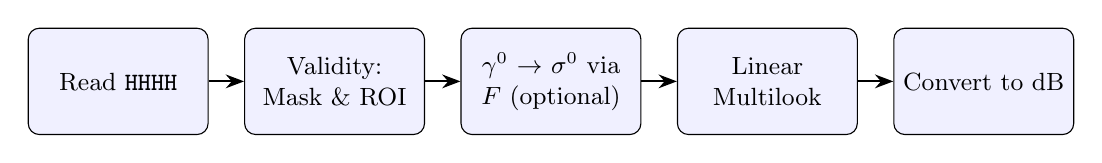
\begin{tikzpicture}[node distance=4.5mm,
  caja/.style={draw,rounded corners,fill=blue!6,align=center,text width=2.05cm,minimum height=1.35cm,font=\small},
  fl/.style={-{Stealth},thick}]
\node[caja] (a) {Read \texttt{HHHH}};
\node[caja,right=of a] (b) {Validity: Mask \& ROI};
\node[caja,right=of b] (c) {$\gamma^0\to\sigma^0$ via $F$ (optional)};
\node[caja,right=of c] (d) {Linear Multilook};
\node[caja,right=of d] (e) {Convert to dB};
\draw[fl] (a)--(b); \draw[fl] (b)--(c); \draw[fl] (c)--(d); \draw[fl] (d)--(e);
\end{tikzpicture}
\caption{The pixel processing pipeline: from raw HDF5 reading to decibel scale. Execution order is critical: spatial averaging is performed \emph{before} converting to decibels.}
\label{fig:recorrido}
\end{figure}

\subsection{Step 1: Reading}

The floating-point value is read directly from the \texttt{HHHH} or \texttt{HVHV} dataset via windowed HDF5 slicing. No scaling is applied: the file already delivers linear backscatter power in the $\gamma^0$ convention. Suppose, as a concrete example, that a single pixel reads $\gamma^0_{HH}=0.158$.

\subsection{Step 2: Validity Masking}

A pixel enters quantitative analysis if and only if its product \texttt{mask} is neither 0 nor 255 and its center falls inside the ROI polygon (Section~\ref{sec:figuras}). Otherwise, it is masked to $\mathrm{NaN}$ and \emph{never} replaced by zero: a zero would falsely imply ``zero returned energy'' and bias spatial averages downward. Across the Stage 1 Chiapas ROI polygon, $99.61\,\mathrm{\%}$ of interior pixels are valid.

\subsection{Step 3: Converting $\gamma^0$ to $\sigma^0$ (When Required)}

Multiplying by the co-registered \texttt{rtcGammaToSigmaFactor} value $F$ at that same pixel (illustrative value: $F=0.74$) yields:
\begin{equation}
  \sigma^0 = \gamma^0F = 0.158\times0.74 = 0.117 .
\end{equation}
In decibels, $\gamma^0_{\mathrm{dB}}=10\log_{10}(0.158)=-8.01$\,dB and $\sigma^0_{\mathrm{dB}}=10\log_{10}(0.117)=-9.32$\,dB; their difference ($-1.31$\,dB) equals $10\log_{10}F$. A factor $F=0.74$ corresponds to $\cos\theta$ at $\theta\approx42^\circ$ over flat terrain; on steep slopes, DEM-derived $F$ can depart significantly from $\cos\theta_i$.

\subsection{Step 4: Linear-Power Multilooking}

Pixels within each $n\times n$ block ($2\times2$ in Stage 1 inspection, $5\times5$ by default in change detection) are averaged in linear power subject to the validity rule $N_v\ge0.5\,n^2$ (Figure~\ref{fig:multilook_bloques} and Table~\ref{tab:bloques}). Averaging in linear units is physically mandatory because electromagnetic energy (not its logarithm) adds across adjacent resolution cells.

\subsection{Step 5: Conversion to Decibels}

Only after spatial averaging is $10\log_{10}\bar P_B$ evaluated. This final dB value drives the rendered rasters (Figures~B and B2) and regional summary statistics.

\begin{cuidado}
Reversing the order---``convert to dB first, average second''---is a widespread implementation error. It produces a systematically lower value (the negative Jensen bias analyzed in Section~\ref{sec:speckle}) whose magnitude depends on the number of looks, rendering measurements incomparable across different multilook settings.
\end{cuidado}

\section{From a Single Pixel to a Region of Interest}
\label{sec:region}

A scientific conclusion rarely rests on a single pixel. Over a Region of Interest, population statistics are evaluated across all valid pixels. In the Stage 1 Chiapas granule, this comprises $n=14,699,442$ valid pixels per polarization at full 10\,m resolution. Table~\ref{tab:stats-roi} compiles the resulting histogram statistics and explains how to interpret each metric.

\begin{table}[htbp]
\centering\small
\begin{tabularx}{\linewidth}{p{.3\linewidth}rrX}
\toprule
\textbf{Statistic} & \textbf{HH} & \textbf{HV} & \textbf{Physical Interpretation}\\\midrule
Mean of dB & $-8.055$ & $-13.503$ & Summarizes the center of the \emph{dB histogram}; not mean physical power.\\
Median (dB) & $-7.880$ & $-13.173$ & Robust central tendency, insensitive to bright point outliers.\\
dB of linear mean & $-3.786$ & $-9.226$ & Corresponds to true mean scattered power; sensitive to bright upper tails.\\
Gap between the two means & $4.27$ & $4.28$ & Measures histogram skewness + speckle (Jensen gap), not temporal change.\\
$p_5$ to $p_{95}$ range (dB) & $-14.07$ to $-2.85$ & $-20.00$ to $-8.11$ & Central 90\,\% dynamic range of the region.\\
Standard deviation (dB) & $3.59$ & $3.73$ & Combined dispersion from residual speckle and landscape heterogeneity.\\\bottomrule
\end{tabularx}
\caption{Full-resolution $\gamma^0$ dB statistics across the Stage 1 Chiapas ROI (HH and HV). Values extracted from \texttt{metadatos.json}.}
\label{tab:stats-roi}
\end{table}

\paragraph{Which Mean Should Be Reported?} It depends on the scientific question. To describe the visual appearance and central location of the log-transformed histogram, report the mean of the dB values or the median. For radiative energy budgets or physical backscatter models, report the \emph{linear} mean converted to dB. Above all, always declare which definition is used, since they differ by $4.3$\,dB in this scene.

\paragraph{What the HH--HV Offset Indicates.} Across this ROI, HV averages $5.4$\,dB lower than HH ($-13.50$ vs.\ $-8.06$\,dB). This matches physical expectation---cross-polarized volume depolarization returns less energy than co-polarized surface and canopy scattering across almost all natural land covers---and is visually confirmed by the shared-scale panels of Figure~B.

\section{A Two-Date Change Example}
\label{sec:ej-dos-fechas}

Consider a small patch observed on two comparable dates where linear power doubles from $P_1=0.10$ to $P_2=0.20$:
\begin{equation}
  \Delta\sigma^0_{\mathrm{dB}}=10\log_{10}\frac{0.20}{0.10}=+3.01\ \text{dB}.
\end{equation}
Does $+3.01$\,dB represent a genuine surface change? That depends entirely on the statistical sample size and number of looks:
\begin{itemize}
  \item For a single pixel at $L=1$ look per date, the difference noise floor is $\sigma_\Delta\approx7.9$\,dB, so $+3.01$\,dB is statistically indistinguishable from random speckle ($z\approx0.4$).
  \item For a single block with $L=4$ independent looks (e.g., an idealized $2\times2$ multilook), $\sigma_\Delta\approx3.3$\,dB ($z\approx0.9$): still within random noise.
  \item Averaging across a homogeneous parcel of 100 independent blocks with $L=4$ reduces the standard error to $\sigma_\Delta\approx0.33$\,dB, placing $+3.01$\,dB at $z\approx9$: now an unmistakable detection \emph{that radar backscatter changed}.
\end{itemize}
Even in the third case, radar statistics alone do not answer \emph{why} it changed. Causal attribution belongs to physical interpretation supported by the scattering models of Section~\ref{sec:modelos} and independent auxiliary datasets.

\begin{atencion}
A raw $\Delta\sigma^0$ map sprinkled with isolated $\pm3$\,dB pixels may look dramatic yet mean nothing: pure independent speckle produces that exact pattern over completely static terrain (Figure~\ref{fig:delta_distribucion}). Before interpreting any change map, always check how many independent looks and contiguous pixels support an anomaly, and verify that the threshold exceeds $3\sigma_{\mathrm{MAD}}$.
\end{atencion}

\section{Pre-Interpretation Quality Checklist}
\label{sec:checklist-radar}

\begin{enumerate}
  \item Do both scenes share the exact same product type, orbital track, frame, flight direction, polarization, spatial resolution, CRID, and maturity level?
  \item Are the UTM pixel grids identical (CRS, affine transform, shape), and was valid polygon coverage verified on both dates?
  \item Was spatial multilooking performed in linear power prior to decibel conversion using the identical validity rule on both dates?
  \item How many independent looks support the measurement, and what is the ROI's empirical noise floor $\sigma_{\mathrm{MAD}}$?
  \item Was the decibel classification threshold $\tau_{\mathrm{dB}}$ verified against the $3\sigma_{\mathrm{MAD}}$ noise-floor criterion?
  \item Is it explicitly stated whether reported averages are means of dB, medians, or dB of linear means?
  \item Does the narrative clearly separate direct radiometric observation from physical inference and model prediction?
  \item Is there independent auxiliary evidence (GPM IMERG precipitation, HLS/Sentinel-2 optical imagery, OPERA products) supporting or refuting the physical hypothesis?
\end{enumerate}

\section{Contrast with Independent Auxiliary Sources}
\label{sec:contraste}

Because $\Delta\gamma^0$ or $\Delta\sigma^0$ alone cannot uniquely identify a physical cause, TerraPulse AI contrasts radar change maps against complementary Earth observation datasets, each carrying its own strengths and limitations (Table~\ref{tab:fuentes-aux}).

\begin{table}[htbp]
\centering\small
\begin{tabularx}{\linewidth}{p{.2\linewidth}p{.32\linewidth}X}
\toprule
\textbf{Auxiliary Source} & \textbf{What It Contributes} & \textbf{Key Limitations}\\\midrule
GPM IMERG & Satellite-estimated precipitation at high temporal cadence on a regional grid. & Coarse spatial resolution ($\approx 10$\,km) relative to 10--50\,m SAR pixels; indirect rain retrieval rather than rain-gauge measurement.\\
HLS / Sentinel-2 (Optical) & Multispectral visible and infrared reflectance (e.g., NDVI, NDWI) for vegetation and open water. & Blocked by cloud cover, which is frequent during tropical storm events.\\
OPERA (DSWx / DIST) & Derived surface water extent and land disturbance products from optical/SAR constellations. & Another derived algorithmic product: comparison measures \emph{inter-product agreement}, not ground-truth accuracy.\\\bottomrule
\end{tabularx}
\caption{Independent auxiliary sources used to contextualize and contrast SAR backscatter changes.}
\label{tab:fuentes-aux}
\end{table}

Effective validation is \emph{spatio-temporal}: comparing the spatial pattern and acquisition dates of the SAR anomaly against the timing and footprint of independent observations, while honestly reporting both agreements and discrepancies. An intense IMERG rainfall event preceding a widespread $\Delta\gamma^0$ shift is consistent with soil wetting or inundation, whereas a cloud-free optical acquisition confirming standing water or an NDVI drop provides stronger corroboration.

\section{Traceability and Reproducibility}
\label{sec:trazabilidad}

Every number produced by Stage 1 and the change pipeline is auditable because the software persists machine-readable provenance alongside every output raster and chart:
\begin{description}[style=nextline]
  \item[\texttt{metadatos.json} / \texttt{change.json}] Input granule IDs, acquisition timestamps, processing parameters, population statistics, noise floor $\sigma_{\mathrm{MAD}}$, and exact Git commit hash (\texttt{version\_codigo}).
  \item[\texttt{control/*.csv}] Tabular numerical outputs backing every static figure; no quantity is ever derived from rendered PNG images.
  \item[Cryptographic Hashes \& Git Version] Content hashes and code version strings. A \texttt{-dirty} suffix flags uncommitted local edits at execution time.
\end{description}
Noting \texttt{98f7e07-dirty} in Section~\ref{sec:figuras} is deliberate scientific hygiene: before publishing final figures, regenerating the output directory from a clean Git working tree ensures that any third party can reproduce the exact same numbers bit-for-bit.

\part{DG2 Flood Simulation by Region of Interest}
\label{part:inundacion}

This part documents the implemented execution path that, upon an authenticated request, transforms a declared Region of Interest (ROI) and computational domain into a \emph{synthetic} rainfall scenario, prepares NASADEM terrain, executes the LISFLOOD-FP 8.0 DG2 CPU solver, and delivers numerical water-depth maps. Three distinct layers are separated throughout: the continuous shallow-water physical model, its second-order Discontinuous Galerkin (DG2) numerical discretization, and the software adapter governing files, worker processes, and REST API endpoints. Every equation identifies physical quantities and SI units, and operational claims are linked directly to source files. An integrable, downloadable simulation output is \emph{not} a validated flood prediction: scientifically defensible domain delineation, inflow hydrographs, spatially distributed roughness, infiltration, verified mass conservation, and independent ground-truth comparison remain prerequisites for real-event studies. No water depth, rainfall rate, or causal attribution is ever derived from NISAR radar data.

\noindent\emph{Documentary specification of the implementation observed on branch} \texttt{simulacion-inundancion}.


\section{Conceptual Guide: From Water in a Single Cell to a Depth Map}
\label{sec:guia-inundacion}

Because the subsequent sections rigorously bind every mathematical expression to its C++ and Python implementation, this opening section provides an intuitive \emph{road map}: what physical problem is being solved, what core numerical ideas make it work, and how a complete hand calculation connects a JSON request to a cubic-meter water volume.

\subsection{The Physical Problem in One Sentence}

When rain falls over terrain, water accumulates in topographic depressions and flows downhill, retarded by bed friction. Whenever water depth is thin compared to horizontal flow distances (decimeters of water across hundreds of meters of terrain), vertical acceleration can be neglected: it suffices to track water depth $h(x,y,t)$ and depth-integrated unit discharge $\mathbf q=(q_x,q_y)$ at every point. This vertically integrated formulation is known as the \textbf{2D Shallow Water Equations} (SWE).

\subsection{The Two Conservation Laws}

Equations~\eqref{eq:conserv}--\eqref{eq:sources} express two fundamental physical balances:
\begin{description}[style=nextline]
  \item[Conservation of Mass (Continuity, first component).] The water volume inside a cell changes solely because water flows across its four lateral faces or falls as rain from above: $\partial_t h+\nabla\!\cdot\!\mathbf q=r$ (Figure~\ref{fig:swe_celda}). In the absence of rainfall and boundary outflow, total water volume across the domain remains constant.
  \item[Conservation of Momentum (second and third components).] Water accelerates under gravity: hydrostatic pressure pushes fluid from deeper toward shallower regions, while bed slope pulls fluid downhill. Bed roughness resists motion through a frictional shear stress that grows quadratically with flow speed.
\end{description}

\figura{swe_celda}{0.95}{Mass balance inside a computational cell of width $\Delta x$. Water depth $h$ is measured vertically from bed elevation $z_b$ to free-surface elevation $\eta=z_b+h$. Unit discharge $q_x$ enters across the left face and exits across the right face, while rainfall rate $r$ adds depth from above.}

\subsection{Physical Meaning of Each Term}

\begin{table}[htbp]
\centering\small
\begin{tabularx}{\linewidth}{p{.24\linewidth}p{.28\linewidth}X}
\toprule
\textbf{Term} & \textbf{Location} & \textbf{Physical Meaning}\\\midrule
$\partial_t\boldsymbol U$ & Left-hand side & Local time rate of change of depth and unit discharge.\\
$\partial_x\mathcal F+\partial_y\mathcal G$ & Left-hand side & Net flux of mass and momentum across cell faces.\\
$q_x^2/h$ & $\mathcal F$, component 2 & Advective momentum transport by the flow itself (inertia).\\
$gh^2/2$ & $\mathcal F$, component 2 & Depth-integrated hydrostatic pressure force.\\
$-gh\,\partial_xz_b$ & $\boldsymbol S_b$ & Gravitational driving force along the bed slope.\\
$-ghS_{f,x}$ & $\boldsymbol S_f$ & Manning bottom friction resistance.\\
$r$ & $\boldsymbol S_r$ & Rainfall source term: adds water depth without horizontal momentum.\\\bottomrule
\end{tabularx}
\caption{Physical translation of each term in the 2D Shallow Water Equations~\eqref{eq:conserv}.}
\label{tab:terminos-swe}
\end{table}

\subsection{Gravity Wave Speed and Why It Governs the Time Step}

In shallow water, small surface disturbances propagate at gravity wave celerity $c=\sqrt{gh}$ relative to the moving fluid. With $g=9.81$\,m/s$^2$: at depth $h=1$\,m, waves travel at $3.13$\,m/s; at $h=0.1$\,m, at $0.99$\,m/s; and in a thin $h=1$\,cm film, at $0.31$\,m/s. The computational consequence is immediate: \emph{deeper water propagates information faster}, forcing an explicit numerical solver to take shorter time steps $\Delta t$ so waves do not skip across an entire grid cell in a single step. This is the physical origin of the Courant--Friedrichs--Lewy (CFL) stability condition (Section~\ref{sec:dg2}).

\subsection{Discretizing the Terrain into Cells: Finite Volumes vs.\ DG2}

Because solving the continuous PDEs analytically over real topography is impossible, the domain is tessellated into rectangular cells of size $\Delta x\times\Delta y$. Classical first-order \emph{Finite Volume} schemes store a single number per field in each cell (the cell average). By contrast, the second-order \textbf{Discontinuous Galerkin} (DG2) scheme implemented in LISFLOOD-FP stores \emph{three} modal coefficients per field in every cell: the cell mean $W_0$ plus two linear slope modes $W_{1x}$ and $W_{1y}$ describing how the variable tilts across the cell interior (Figure~\ref{fig:dg2_base}). Representing each cell by ``an average height plus a planar tilt'' captures water-surface gradients and topographic slopes with substantially higher fidelity on the same grid resolution.

\figura{dg2_base}{0.7}{Modal DG2 representation inside a 1D cell. The true continuous profile (gray) is approximated by a piecewise linear function (blue); $W_0$ is the cell mean and $W_{1x}$ controls the slope. Face values are $W_0\pm\sqrt{3}\,W_{1x}$ (circles) and internal Gauss quadrature points are $W_0\pm W_{1x}$ (squares).}

\subsection{Three Core Numerical Ingredients in Plain Language}

\paragraph{1. Inter-Cell Fluxes (HLL Riemann Solver).} At every shared face between two cells, the piecewise linear reconstructions generally meet at a jump discontinuity (a left state $U_L$ and a right state $U_R$). The HLL (Harten--Lax--van Leer) approximate Riemann solver computes the mass and momentum flux crossing that face by bounding the local wave fan between two extreme acoustic speeds $S^-$ and $S^+$ (Figure~\ref{fig:hll_abanico}).

\figura{hll_abanico}{0.55}{Structure of the HLL approximate Riemann fan at a cell interface. Two bounding wave speeds ($S^-$ and $S^+$) separate the left state $U_L$, an intermediate state $U^*$, and the right state $U_R$.}

\paragraph{2. Wet--Dry Fronts (Hydrostatic Reconstruction).} A critical challenge in flood modeling occurs at shoreline boundaries where a wet cell abuts a dry cell sitting at higher elevation. Naive flux evaluation would create artificial uphill flow or negative water depths. \emph{Hydrostatic reconstruction} (Figure~\ref{fig:reconstruccion_hidro}) references both sides of the interface to a common sill elevation $z^*=\max(z_b^-,z_b^+)$ and defines effective face depths $h^*=\max(0,\eta-z^*)$: if the water surface $\eta$ lies below the neighboring dry bed elevation, the effective depth vanishes and zero spurious flux is generated.

\figura{reconstruccion_hidro}{0.78}{Hydrostatic reconstruction at a wet--dry interface. The left cell is wet while the right cell is dry with a higher bed elevation. The effective right-hand depth evaluates to $0$, preventing unphysical uphill flux.}

\paragraph{3. Time Stepping (RK2 and CFL).} The solver advances modal coefficients in time using a two-stage Runge--Kutta (RK2) scheme while dynamically restricting $\Delta t$ so that no wave traverses more than a fraction $C_{\mathrm{CFL}}=0.33$ of a cell per step (Figure~\ref{fig:cfl_dt}).

\figura{cfl_dt}{0.66}{CFL stability time-step limit for 20\,m grid cells with $C_{\mathrm{CFL}}=0.33$. In a 1\,cm film, $\Delta t_{\max}\approx21$\,s; at $h=1$\,m still water, $2.1$\,s; at $h=0.1$\,m with flow speed $0.5$\,m/s, $4.4$\,s.}

\begin{ejemplo}[Hand Calculation of the CFL Time Step]
For $h=0.1$\,m, $|u|=0.5$\,m/s, and $\Delta x=20$\,m:
\[
  \Delta t\le C_{\mathrm{CFL}}\frac{\Delta x}{|u|+\sqrt{gh}}
  =0.33\,\frac{20}{0.5+\sqrt{9.81\times0.1}}
  =\frac{6.6}{0.5+0.990}=4.43\ \text{s}.
\]
In the illustrative API request below (a 2\,s test run with $\Delta t_{\text{initial}}=0.1$\,s), the user-prescribed initial step $0.1$\,s is already smaller than $4.43$\,s, so the $\min(\Delta t_{\text{initial}},\ldots)$ cap governs.
\end{ejemplo}

\subsection{Manning Friction: Physical Intuition}

Manning's roughness coefficient $n_M$ quantifies surface resistance to flow: low values ($0.02\,\text{s/m}^{1/3}$) represent smooth bare earth or concrete, whereas high values ($0.08$ or above) represent dense floodplain vegetation. Frictional resistance grows with the square of flow speed and inversely with depth ($h^{-1/3}$ in the friction factor $C_f$, $h^{-4/3}$ in the friction slope $S_f$): the shallower the sheet flow, the more strongly bed roughness dominates fluid motion (Figure~\ref{fig:manning_friccion}).

\figura{manning_friccion}{1.0}{Left: dimensionless friction factor $C_f=gn_M^2/h^{1/3}$ vs.\ water depth $h$ for three Manning $n_M$ values. Right: friction slope $S_f$ at flow speed $u=1$\,m/s. At identical $n_M$, bed resistance increases sharply in thin water films.}

\begin{ejemplo}[Friction Head Loss in a 10\,cm Water Sheet]
With $n_M=0.02\,\text{s/m}^{1/3}$, $h=0.1$\,m, and $u=1$\,m/s, the dimensionless friction factor is
$C_f=9.81\times0.02^2/0.1^{1/3}=0.00845$ and the friction slope is
$S_f=n_M^2u^2/h^{4/3}=0.0004/0.0464=0.0086$, corresponding to $8.6$\,mm of energy head loss per meter of horizontal travel.
\end{ejemplo}

\subsection{From an API Request to a Water Volume: Complete Worked Example}
\label{sec:ej-lluvia}

Using the illustrative request parameters from Section~\ref{sec:vida}, we can trace how a JSON rainfall specification translates into total water volume:

\begin{enumerate}
  \item \textbf{Accumulated Depth and Duration.} $P=2$\,mm over $T_r=1$\,s. The mean rainfall rate is
        $\bar{r}=P/T_r=0.002$\,m/s (equivalent to $0.002\times1000\times3600=7200$\,mm/h---mathematically consistent for a fast unit test, though physically extreme).
  \item \textbf{Balanced Temporal Intervals.} With $N=2$ intervals of $0.5$\,s each, the maximum perturbation amplitude is
        $\delta=\min(10\text{ mm/h},\bar{r})=10\text{ mm/h}=2.78\times10^{-6}$\,m/s, which is negligible compared to $\bar{r}$: both intervals apply virtually $0.002$\,m/s.
  \item \textbf{Depth Added per Cell.} Every cell center falling inside the ROI polygon receives $\sum r_k\Delta t_r = 2$\,mm ($0.002$\,m) of water depth.
  \item \textbf{Volume per ROI Cell.} At $\Delta x=\Delta y=20$\,m resolution, cell area is $\Delta A=400$\,m$^2$, so each wet ROI cell receives $0.002\ \text{m}\times400\ \text{m}^2=0.8$\,m$^3$ of water.
  \item \textbf{Total Injected Volume.} Multiplying $0.8$\,m$^3$ by the number of cell centers inside the ROI ($N_{\mathrm{ROI}}$; e.g., $3.2$\,m$^3$ for $N_{\mathrm{ROI}}=4$) gives the exact nominal volume injected into the domain.
\end{enumerate}

\figura{malla_dominio}{0.78}{Computational grid layout. The user ROI (green) and enclosing hydraulic domain (dashed blue) are reprojected to a metric UTM CRS; the aligned computational rectangle (black) adds a 2-cell margin on all sides. Rainfall is injected exclusively at cell centers (green dots) lying inside the ROI polygon.}

\figura{lluvia_perfil}{0.7}{Illustration of the \texttt{uniform\_balanced} temporal rainfall profile (10 intervals oscillating around a 20\,mm/h mean): symmetric $\pm d_j$ pairs cancel exactly so the integrated rainfall depth matches the prescribed 20\,mm total.}

\begin{intuicion}
The \texttt{uniform\_balanced} profile generator introduces controlled temporal variability without altering the \emph{prescribed total depth}: perturbations are drawn in symmetric pairs $\pm d_j$ that sum to zero by construction (Equation~\eqref{eq:rainbal}).
\end{intuicion}

\subsection{Which Question Each Platform Module Answers}

\begin{table}[htbp]
\centering\small
\begin{tabularx}{\linewidth}{p{.25\linewidth}p{.28\linewidth}X}
\toprule
\textbf{Module} & \textbf{Question Answered} & \textbf{What It Does \emph{Not} Answer}\\\midrule
SAR Radar (Parts~\ref{part:fundamentos}--\ref{part:pixel}) & Did L-band radar backscatter change between two dates? & The underlying physical cause of the change.\\
Flood Simulator (this part) & Under this hypothetical rainfall and DEM, where does surface water accumulate? & Where flooding \emph{actually} occurred in reality, or calibrated hazard forecasting.\\
Solar Simulator (Part~\ref{part:solar}) & How much clear-sky direct beam irradiance strikes each DEM facet at this timestamp? & Cloud-attenuated real irradiance or diffuse sky radiation.\\\bottomrule
\end{tabularx}
\caption{Strict epistemic boundaries across platform modules.}
\label{tab:modulos}
\end{table}


\section{Reading Guide and Operational Scope}
\label{sec:alcance}
\begin{center}
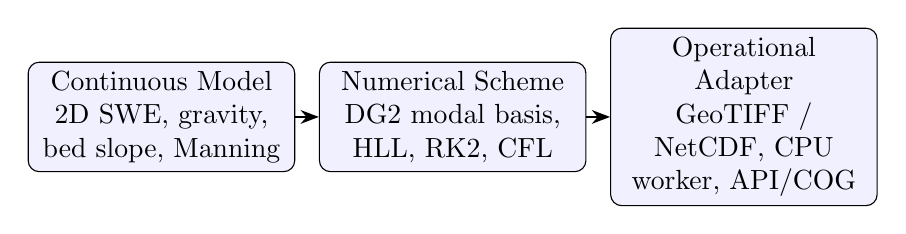
\begin{tikzpicture}[node distance=3mm,box/.style={draw,rounded corners,fill=blue!6,align=center,text width=3.15cm,minimum height=1.3cm},arr/.style={-{Stealth},thick}]
\node[box] (a) {Continuous Model\\2D SWE, gravity, bed slope, Manning};
\node[box,right=of a] (b) {Numerical Scheme\\DG2 modal basis, HLL, RK2, CFL};
\node[box,right=of b] (c) {Operational Adapter\\GeoTIFF / NetCDF, CPU worker, API/COG};
\draw[arr] (a)--(b); \draw[arr] (b)--(c);
\end{tikzpicture}
\end{center}
\noindent\textbf{Question and Answer.} What does the implemented ROI flood pipeline compute? It computes surface water depth $h$, in meters \emph{above the local bed}, across a rectangular metric grid under user-prescribed hypothetical rainfall applied uniformly across ROI cell centers, starting from an initially dry bed with constant Manning roughness and idealized domain boundaries. Output rasters represent scheduled time frames and the maximum depth envelope; they are not satellite-observed flood maps. The API does not return flow velocity vectors, wave arrival timestamps, or validated inundation extents.

The workflow is restricted to user-declared non-urban terrain (\texttt{domain\_nonurban:true} is an explicit caller declaration, not an automated land-cover classifier). A small visualization ROI rarely encompasses the full contributing hydrological catchment; the caller must supply an enclosing \texttt{domain} polygon large enough to contain relevant upslope inflows and downslope outlets. Storm drains, culverts, buildings, sub-grid channel bathymetry, and subsurface infiltration are not modeled. The active per-ROI runner is \src{pipeline/hydrology/roi_runner.py}, which is independent of the validation-only \texttt{prepare/} endpoint.

\warn{Passing schema validation and completing solver execution does not constitute hydraulic validation. Numerical values in the API example below are purely illustrative test payloads, not recommended physical parameters or observed events.}

\section{Physical Quantities, Reference Datums, and Assumptions}
\label{sec:simbolos}
Let $(x,y)$ denote projected horizontal coordinates in meters (never degrees), $t$ time in seconds from the \emph{simulated} start, and $z_b(x,y)$ stationary bed elevation in meters above a declared vertical datum. Water depth $h(x,y,t)\geq0$ is measured vertically \emph{above the local bed} $z_b$, whereas free-surface elevation $\eta=z_b+h$ is referenced to the \emph{same} vertical datum. NASADEM\_HGT supplies orthometric elevations referenced to the EGM96 geoid; horizontal UTM reprojection does not alter the vertical datum. Velocities $u,v$ are depth-averaged horizontal velocity components in m/s, and $g$ is gravitational acceleration in m/s$^2$.

Unit discharges $q_x=hu$ and $q_y=hv$ have units of m$^2$/s (volume flux per unit width normal to the flow). Total volumetric discharge across a section of width $B$ is $Q=\int_B\boldsymbol q\cdot\boldsymbol n_{\!f}\,\dd\ell$ in m$^3$/s, where $\boldsymbol n_{\!f}$ is the horizontal unit normal vector (distinct from Manning's coefficient $n_M$). Dividing $Q$ by wetted cross-sectional area $A_c$ gives mean flow speed $Q/A_c$ (m/s), whereas dividing by horizontal planform area $A_p$ gives an equivalent areal depth rate $Q/A_p$ (m/s). The symbol $q_s$ denotes a generic areal depth source (m/s), never $q_x$ or $Q$.

\begin{longtable}{p{.18\linewidth}p{.17\linewidth}p{.57\linewidth}}
\toprule Symbol & SI Unit & Reference, Denominator, and Physical Interpretation\\\midrule\endhead
$h,z_b,\eta$ & m & Water depth above local bed; bed elevation and free-surface elevation above a common vertical datum ($\eta-z_b=h$).\\
$x,y,\Delta x,\Delta y$ & m & Projected horizontal coordinates and grid cell dimensions in meters.\\
$t,\Delta t$ & s & Simulated elapsed time and computational time step (no implied wall-clock UTC timestamp).\\
$u,v,c=\sqrt{gh}$ & m/s & Depth-averaged horizontal velocity components and shallow-water gravity wave speed.\\
$q_x,q_y$ & m$^2$/s & Volumetric discharge \emph{per unit width} across a vertical plane.\\
$Q$ & m$^3$/s & Total volumetric discharge across a full cross-section.\\
$r,i,q_s$ & m/s & Areal rainfall rate, infiltration loss rate, and net areal source per unit \emph{horizontal planform area and time}: m$^3$/(m$^2$\,s). ($i,q_s$ are not active in the ROI API).\\
$n_M$ & s/m$^{1/3}$ & Manning roughness coefficient in SI units (explicitly required in the request).\\
$S_{f,x},S_{f,y}$ & 1 & Dimensionless friction slope (energy head loss per unit horizontal distance, carrying velocity sign).\\
$\mathcal F,\mathcal G$ & (m$^2$/s, m$^3$/s$^2$, m$^3$/s$^2$) & Conserved mass flux per unit width (component 1) and depth-integrated momentum fluxes (components 2--3).\\
$\Delta A=\Delta x\Delta y$ & m$^2$ & Horizontal planform area of a grid cell.\\\bottomrule
\end{longtable}

The 2D shallow-water formulation integrates over the vertical column under a hydrostatic pressure distribution, valid when horizontal scales greatly exceed depth. It does not resolve 3D vertical vorticity or sub-grid hydraulic structures, and remeshing a 30\,m DEM onto a finer grid does not recover unmeasured channel bathymetry.

\section{Continuous Governing Equations and Conservation Form}
\label{sec:ecuaciones}
For the conserved state vector $\boldsymbol U=(h,q_x,q_y)^{\mathrm T}$, the 2D conservative system is
\begin{align}
\partial_t\boldsymbol U+\partial_x\mathcal F(\boldsymbol U)+\partial_y\mathcal G(\boldsymbol U)&=\boldsymbol S_b+\boldsymbol S_f+\boldsymbol S_r,\label{eq:conserv}\\
\mathcal F&=\begin{pmatrix}q_x\\ q_x^2/h+gh^2/2\\q_xq_y/h\end{pmatrix},\qquad
\mathcal G=\begin{pmatrix}q_y\\q_xq_y/h\\q_y^2/h+gh^2/2\end{pmatrix},\label{eq:flux}\\
\boldsymbol S_b&=\begin{pmatrix}0\\-gh\partial_xz_b\\-gh\partial_yz_b\end{pmatrix},\quad
\boldsymbol S_r=\begin{pmatrix}r\\0\\0\end{pmatrix},\quad
\boldsymbol S_f=\begin{pmatrix}0\\-ghS_{f,x}\\-ghS_{f,y}\end{pmatrix}.\label{eq:sources}
\end{align}
When $h\to 0$, quotient terms in \eqref{eq:flux} are regularized via wet--dry depth thresholds and hydrostatic face reconstruction. In the active DG2 execution path, rainfall $r$ enters the continuity equation without injecting horizontal momentum, and neither infiltration $i$ nor external point/areal sources $q_s$ are invoked.

\subsection{Term-by-Term Dimensional Verification}
In the continuity equation, $[\partial_t h]=\unit{m/s}$ and $[\partial_xq_x]=[\partial_yq_y]=(\unit{m^2/s})/\unit m=\unit{m/s}$. Because rainfall rate $r$ is defined per unit \emph{planform area}, $r\Delta A\Delta t$ has units of m$^3$. Any rainfall intensity in mm/h must be divided by $1000\times 3600$ before entering \eqref{eq:sources}.

In the momentum equations, $[\partial_t q_x]=\unit{m^2/s^2}$. Both $[q_x^2/h]=(\unit{m^2/s})^2/\unit m=\unit{m^3/s^2}$ and $[gh^2]=\unit{m^3/s^2}$ yield $\unit{m^2/s^2}$ upon differentiation with respect to $x$ or $y$. Because bed slope $\partial_xz_b$ and friction slope $S_{f,x}$ are dimensionless (m/m), both $[-gh\partial_xz_b]$ and $[-gh S_{f,x}]$ carry units of $\unit{m^2/s^2}$.

\subsection{Manning Friction Slope and the Split Implicit Discrete Operator}
With flow speed $w=\sqrt{u^2+v^2}$ (m/s), the continuous Manning friction slopes and momentum source vector are
\begin{equation}
 S_{f,x}=\frac{n_M^2uw}{h^{4/3}},\quad S_{f,y}=\frac{n_M^2vw}{h^{4/3}},\qquad
 \boldsymbol S_{f,\mathrm{mom}}=-\frac{g n_M^2}{h^{1/3}}(uw,vw)^{\mathrm T}.\label{eq:mann}
\end{equation}
Dimensionally, $[n_M^2uw/h^{4/3}]=(\unit{s^2/m^{2/3}})(\unit{m^2/s^2})/\unit{m^{4/3}}=1$, and the friction coefficient $C_f=gn_M^2/h^{1/3}$ is likewise dimensionless: $(\unit{m/s^2})(\unit{s^2/m^{2/3}})/\unit{m^{1/3}}=1$. Note that $C_fuw$ has units of m$^2$/s$^2$, whereas $S_{f,x}$ is dimensionless; in the native C++ source \src{swe/dg2/friction.cpp}, the local variable named \texttt{Sfx} actually stores the momentum source term $-C_fuw$ rather than the dimensionless energy slope $S_{f,x}$ of \eqref{eq:mann}.

To prevent numerical stiffness in very shallow water, the native solver applies an implicit point-wise friction update to cell averages and Gauss quadrature evaluations:
\begin{align}
 C_f&=gn_M^2/h^{1/3}, & D_x&=1+\Delta t\frac{C_f}{h}\frac{2u^2+v^2}{w},
 & D_y&=1+\Delta t\frac{C_f}{h}\frac{u^2+2v^2}{w},\label{eq:fricden}\\
 q_x^{\mathrm{new}}&=q_x+\Delta t\frac{-C_fuw}{D_x}, &
 q_y^{\mathrm{new}}&=q_y+\Delta t\frac{-C_fvw}{D_y}.\label{eq:fricdisc}
\end{align}
Here $[\Delta t(C_f/h)(u^2/w)]=\unit s(1/\unit m)(\unit{m/s})=1$, so denominators $D_x,D_y$ are dimensionless and the increments added to $q_x,q_y$ have units of $\unit{m^2/s}$. Division is bypassed whenever $h\leq\texttt{DepthThresh}$ or both velocity components fall below \texttt{SpeedThresh}. \textbf{This friction operator is operator-split outside the two RK2 stages} (Reference: \src{runtime/source/swe/dg2/friction.cpp}, functions \texttt{apply\_friction} and \texttt{friction}).

\section{From Continuous SWE to the DG2 Discretization}
\label{sec:dg2}
\subsection{Modal Basis and Terrain Projection}
Let $K_{ij}$ be a rectangular grid cell of dimensions $\Delta x,\Delta y$ centered at $(x_i,y_j)$, with dimensionless local coordinates $\xi=2(x-x_i)/\Delta x \in [-1,1]$ and $\zeta=2(y-y_j)/\Delta y \in [-1,1]$. Within each cell, every field $W\in\{h,q_x,q_y,z_b\}$ is approximated by the planar modal expansion:
\begin{equation}
 W_h(x,y)=W_0+\sqrt3 W_{1x}\xi+\sqrt3 W_{1y}\zeta.\label{eq:basis}
\end{equation}
Here $W_0$ is the cell average and $W_{1x},W_{1y}$ are modal slope amplitudes carrying \emph{the exact same physical units as $W$} (the spatial derivative is $\partial_xW_h=2\sqrt3W_{1x}/\Delta x$). Along each axis, this orthogonal Legendre basis evaluates to $W_0\pm\sqrt3W_{1x}$ at the cell faces ($\xi=\pm 1$) and to $W_0\pm W_{1x}$ at the two internal Gauss quadrature nodes ($\xi=\pm 1/\sqrt3$), as implemented in \src{swe/dg2/modifiedvars.cpp} (\texttt{limit\_neg/pos} and \texttt{gauss\_lower/upper}).

The official preprocessor \texttt{generateDG2DEM} reads vertex elevation samples NW, NE, SW, and SE from \texttt{terrain.dem.raw} and projects them onto the modal basis via:
\begin{equation}
 z_0=\frac{NW+NE+SW+SE}{4},\quad
 z_{1x}=\frac{NE+SE-NW-SW}{4\sqrt3},\quad
 z_{1y}=\frac{NE+NW-SE-SW}{4\sqrt3}.\label{eq:vertices}
\end{equation}
All three DEM files (\texttt{.dem}, \texttt{.dem1x}, \texttt{.dem1y}) carry units of meters (EGM96). Our Python adapter rejects any DEM containing voids or sentinel values ($-9999$, $10^{10}$) and passes \texttt{nodata\_elevation 10000000000} so coastal zero-elevation cells are never mistaken for NoData (see \src{preprocess/generateDG2DEM.cpp}, \src{swe/dg2/fields.cpp}, and \src{pipeline/hydrology/dem_dg2.py}).

\subsection{Weak Form, Spatial Residuals, and Hydrostatic Reconstruction}
Multiplying the conservation law by each test basis function $\phi_a \in \{1,\sqrt3\xi,\sqrt3\zeta\}$ and integrating by parts over cell $K$ yields the weak modal form:
\begin{equation}
 \int_K \phi_a\,\partial_t U_h\,\dd A =
 \int_K\!\bigl(\mathcal F(U_h)\partial_x\phi_a+\mathcal G(U_h)\partial_y\phi_a+\phi_a S_b\bigr)\dd A
 -\int_{\partial K}\!\phi_a\widehat{\mathcal H}(U_h^-,U_h^+;\boldsymbol n_{\!f})\dd\ell.
 \label{eq:weak}
\end{equation}
For the cell-average depth mode ($\phi_0 = 1$), the volume integral of the flux derivative vanishes and the spatial residual $L_0(h)$ reduces to the net face flux balance:
\begin{equation}
 L_0(h)=-\frac{\widehat{F}^h_E-\widehat{F}^h_W}{\Delta x}
          -\frac{\widehat{G}^h_N-\widehat{G}^h_S}{\Delta y}.\label{eq:mean}
\end{equation}
For the linear slope modes (\texttt{L1x}, \texttt{L1y}), the volume integral is nonzero and is evaluated at the internal Gauss quadrature points together with face fluxes and modal bed-slope source terms (\texttt{bed\_source\_0x/0y/1x/1y} in \src{swe/dg2.cpp}). Whenever a cell falls below \texttt{thin\_depth}, linear slope increments are zeroed out in $L$.

At every cell interface between left ($-$) and right ($+$) modal reconstructions, \src{swe/dg2/modifiedvars.cpp} performs hydrostatic reconstruction: it sets $z^*=\max(z_b^-,z_b^+)$ and defines non-negative modified face depths $h^*=\max(0,\eta^{\pm}-z^*)$, scaling unit discharges as $q^*=h^*(q/h)$ when wet and $q^*=0$ otherwise.

\subsection{HLL Numerical Flux and Transverse Momentum Component}
Across each interface, a 1D normal Riemann problem is solved using the hydrostatically reconstructed states. When $S^-<0<S^+$, the HLL flux for depth and normal momentum is:
\begin{equation}
 \widehat F_{\mathrm{HLL}}^{(h,q_\perp)}=
 \frac{S^+F_L^{(h,q_\perp)}-S^-F_R^{(h,q_\perp)}
       +S^-S^+(U_R-U_L)^{(h,q_\perp)}}{S^+-S^-},\label{eq:hll}
\end{equation}
reducing to $F_L$ when $S^-\geq0$ and $F_R$ when $S^+<0$. Wave speeds $S^{\pm}$ (m/s) bound the characteristic speeds $u\pm\sqrt{gh}$ with dry-bed branches. In the intermediate fan $S^-<0<S^+$, \emph{the transverse momentum flux is not computed by plugging the third component into \eqref{eq:hll}}: instead, the native solver (\src{swe/hll_include.h}, \src{swe/flux.cpp}) upwinds the tangential velocity across the middle contact wave multiplying the central HLL mass flux $\widehat F_{\mathrm{HLL}}^{(h)}$.

\subsection{Two-Stage RK2 Time Integration and CFL Stability Bounds}
Denoting the 9-component spatial residual vector (fluxes plus bed slope) by $L(U)$, the solver advances via Heun's two-stage Runge--Kutta scheme:
\begin{equation}
 U^{(1)}=U^n+\Delta t L(U^n),\qquad
 U^{n+1}=\tfrac12\bigl(U^n+U^{(1)}+\Delta t L(U^{(1)})\bigr).\label{eq:rk}
\end{equation}
Within each main loop iteration of \texttt{dg2::solve} (\src{swe/dg2.cpp}), execution proceeds in the following strict order: (1) rainfall depth injection $h \mathrel{+}= r\Delta t$ using the \emph{currently active} $\Delta t$, (2) boundary condition update, (3) adaptive CFL $\Delta t$ recalculation, (4) implicit Manning friction update, (5) \texttt{rk\_stage1} and \texttt{rk\_stage2}, and (6) maximum-envelope tracking, time advance $t \mathrel{+}= \Delta t$, and frame output if a save threshold is reached.

Under adaptive time-stepping (\texttt{adaptive\_ts = ON} by default in \src{lisflood.cpp}), $\Delta t$ is bounded across all wet cells by:
\begin{equation}
 \Delta t\leq\min\!\left(\Delta t_{\mathrm{initial}},
 C_{\mathrm{CFL}}\frac{\Delta x}{|u|+\sqrt{gh}},
 C_{\mathrm{CFL}}\frac{\Delta y}{|v|+\sqrt{gh}}\right),\label{eq:cfl}
\end{equation}
with default $C_{\mathrm{CFL}}=0.33$ and $\texttt{DepthThresh}=0.001$\,m (\src{pars.cpp}, \src{swe/dg2.cpp}).

\section{Synthetic Rainfall: From JSON Request to NetCDF Forcing}
\label{sec:lluvia}
The request payload accepts either accumulated rainfall depth $P$ and duration $T_r$, or rainfall intensity and duration; \src{pipeline/hydrology/inputs.py} normalizes both modes to total depth $P$ (m), duration $T_r$ (s), and mean rate $\bar{r}=P/T_r$ (m/s), converting mm/h via $r_{\mathrm{m/s}}=r_{\mathrm{mm/h}}/(1000\cdot3600)$.

Given an \emph{even} number $N$ of equal sub-intervals $\Delta t_r=T_r/N$, the \texttt{uniform\_balanced} profile generator draws $N/2$ perturbations $d_j\sim\mathcal U[-\delta,\delta]$ along with their exact negatives $-d_j$, shuffles the $N$ values using the caller's deterministic \texttt{seed}, and sets $\delta=\min(10/(1000\cdot 3600)\ \unit{m/s},\,\bar{r})$. Consequently, every interval rate $r_k=\bar{r}+d_k\geq0$ is non-negative and the nominal depth sum is conserved exactly:
\begin{equation}
 \sum_{k=0}^{N-1}r_k\Delta t_r
 =N\bar{r}\frac{T_r}{N}+\Delta t_r\sum_kd_k=P.\label{eq:rainbal}
\end{equation}
Each interval rate $r_k$ is applied uniformly to all \emph{grid cell centers} falling inside the ROI polygon and set to zero outside (\src{pipeline/hydrology/rainfall.py}, \src{pipeline/hydrology/rainfall_netcdf.py}).

The NetCDF exporter writes a 64-bit offset NetCDF3 file containing the 3D array \texttt{rainfall\_depth(time,y,x)} storing \emph{accumulated millimeters per interval} $R_k=1000\,r_k\Delta t_r$ (not m/s), with \texttt{time} in hours from zero, $x$ ascending, and $y$ descending, appending zero-rain sentinel frames at the end of the storm and at the end of the simulation. The native reader \src{rain/rain.tpp} converts $R_k$ back to a rate in m/s and increments cell depth via:
\begin{equation}
 r_k=\frac{R_k}{1000\,[3600(t_{k+1}^{\rm h}-t_k^{\rm h})]}\quad\unit{m/s},
 \qquad \Delta h=r_k\Delta t.\label{eq:ncrain}
\end{equation}

\section{Terrain Preparation, Computational Domain, Boundaries, and Initial State}
\label{sec:entradas}
\subsection{From NASADEM to the Metric Computational Grid}
Both \texttt{roi} and \texttt{domain} arrive as \texttt{EPSG:4326} GeoJSON polygons, where \texttt{domain} must spatially cover \texttt{roi}. After projecting both into the caller-specified metric CRS (e.g., \texttt{EPSG:32615}), \src{pipeline/hydrology/roi_runner.py} snaps the bounding box to integer multiples of cell resolution and pads it by 2 cells on all four sides to form a complete rectangular grid.

\src{pipeline/elevation/nasadem.py} acquires the intersecting 1-arcsecond \texttt{NASADEM\_HGT v001} granules, \src{pipeline/hydrology/dem_prepared.py} extracts the elevation mosaic, and \texttt{roi\_runner} resamples elevations onto the metric cell centers. Any void or non-finite sample aborts preparation without inventing terrain. Finally, \texttt{prepare\_dg2\_dem} generates the three modal DEM rasters (\texttt{.dem}, \texttt{.dem1x}, \texttt{.dem1y}) with SHA-256 provenance hashes.

\subsection{Idealized Boundary Conditions and Dry Initial State}
Setting \texttt{initial\_condition: "dry\_zero\_velocity"} prescribes $h(x,y,0)=q_x(x,y,0)=q_y(x,y,0)=0$ everywhere. For domain boundaries, \texttt{closed} uses the native default \texttt{NONE} (reflective zero-normal-flux walls), whereas \texttt{free} causes \src{pipeline/hydrology/boundaries.py} to write \texttt{FREE} across all four outer edges (zero-gradient extrapolation in \texttt{set\_boundary\_values}). Infiltration is explicitly declared as \texttt{infiltration: "unsupported"}.

\section{Operational Lifecycle and Private REST API}
\label{sec:vida}
\begin{center}
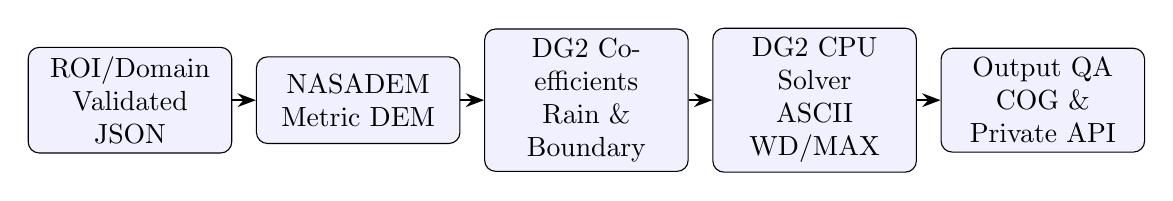
\begin{tikzpicture}[node distance=3mm,box/.style={draw,rounded corners,fill=blue!6,align=center,text width=2.35cm,minimum height=1.1cm},arr/.style={-{Stealth},thick}]
\node[box] (r) {ROI/Domain\\Validated JSON};
\node[box,right=of r] (d) {NASADEM\\Metric DEM};
\node[box,right=of d] (f) {DG2 Coefficients\\Rain \& Boundary};
\node[box,right=of f] (s) {DG2 CPU Solver\\ASCII WD/MAX};
\node[box,right=of s] (c) {Output QA\\COG \& Private API};
\draw[arr] (r)--(d);\draw[arr] (d)--(f);\draw[arr] (f)--(s);\draw[arr] (s)--(c);
\end{tikzpicture}
\end{center}

\subsection{Diagram A: From Authenticated Request to Downloadable Depth COG}
\label{sec:flujo-api}
The end-to-end execution lifecycle separates \emph{admission} (Steps 1--3), \emph{preparation} (Steps 4--6), \emph{solver execution} (Step 7), and \emph{verification \& private publication} (Steps 8--9). Lateral red boxes represent controlled failure exits that never expose partial or unverified rasters. Diagram~B expands Step~7.
\begin{center}
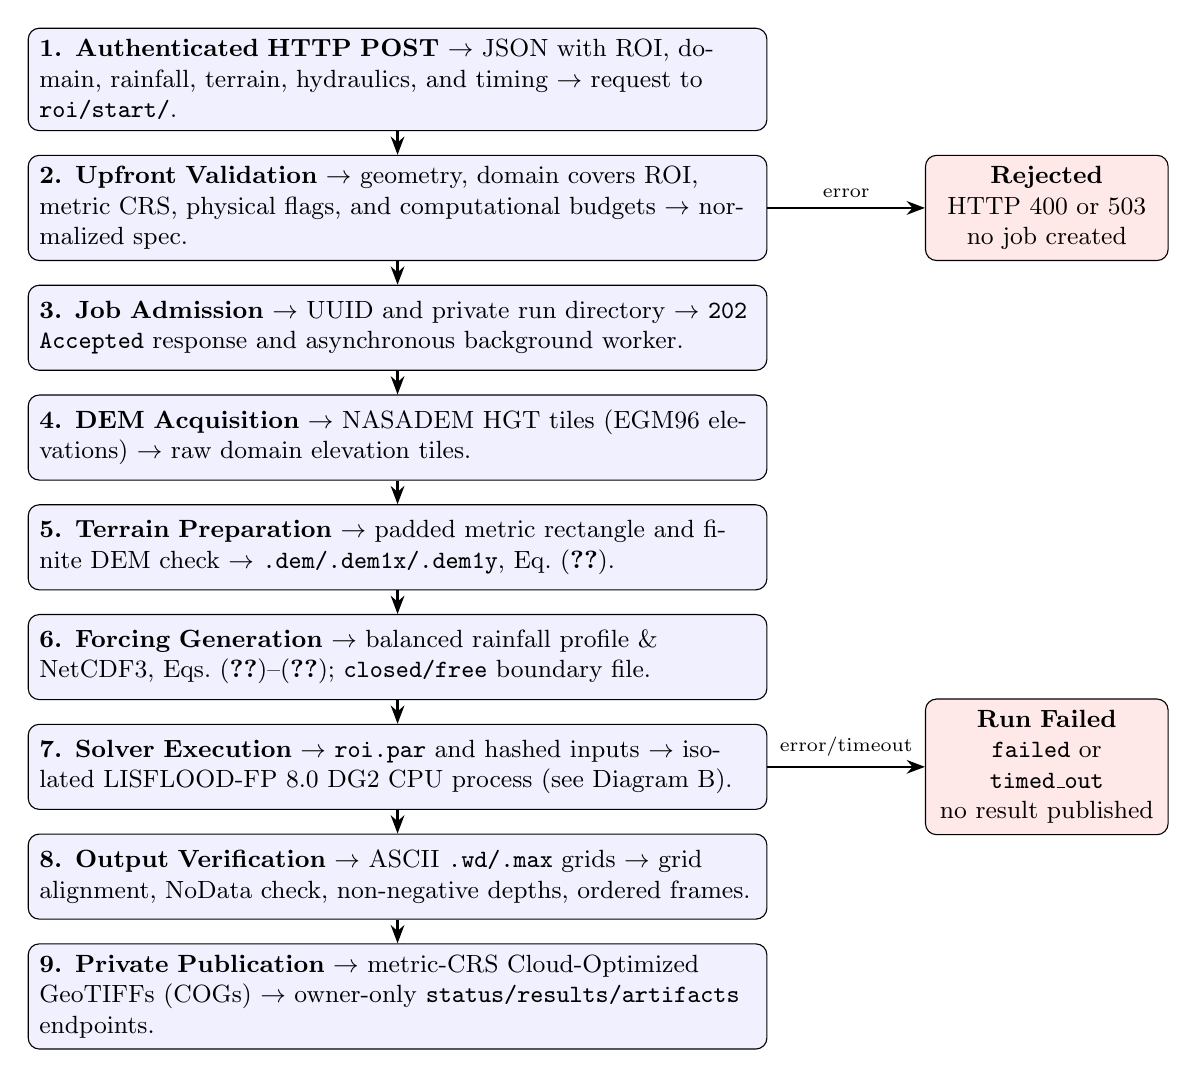
\begin{tikzpicture}[
 node distance=3mm,
 paso/.style={draw,rounded corners,fill=blue!6,align=left,text width=9.1cm,
              minimum height=1.08cm,inner sep=4pt,font=\small},
 fallo/.style={draw,rounded corners,fill=red!9,align=center,text width=2.8cm,
               inner sep=4pt,font=\small},
 flecha/.style={-{Stealth},thick}]
\node[paso] (a1) {\textbf{1. Authenticated HTTP POST} $\to$ JSON with ROI, domain, rainfall, terrain, hydraulics, and timing $\to$ request to \texttt{roi/start/}.};
\node[paso,below=of a1] (a2) {\textbf{2. Upfront Validation} $\to$ geometry, domain covers ROI, metric CRS, physical flags, and computational budgets $\to$ normalized spec.};
\node[paso,below=of a2] (a3) {\textbf{3. Job Admission} $\to$ UUID and private run directory $\to$ \texttt{202 Accepted} response and asynchronous background worker.};
\node[paso,below=of a3] (a4) {\textbf{4. DEM Acquisition} $\to$ NASADEM HGT tiles (EGM96 elevations) $\to$ raw domain elevation tiles.};
\node[paso,below=of a4] (a5) {\textbf{5. Terrain Preparation} $\to$ padded metric rectangle and finite DEM check $\to$ \texttt{.dem/.dem1x/.dem1y}, Eq.~\eqref{eq:vertices}.};
\node[paso,below=of a5] (a6) {\textbf{6. Forcing Generation} $\to$ balanced rainfall profile \& NetCDF3, Eqs.~\eqref{eq:rainbal}--\eqref{eq:ncrain}; \texttt{closed/free} boundary file.};
\node[paso,below=of a6] (a7) {\textbf{7. Solver Execution} $\to$ \texttt{roi.par} and hashed inputs $\to$ isolated LISFLOOD-FP 8.0 DG2 CPU process (see Diagram B).};
\node[paso,below=of a7] (a8) {\textbf{8. Output Verification} $\to$ ASCII \texttt{.wd/.max} grids $\to$ grid alignment, NoData check, non-negative depths, ordered frames.};
\node[paso,below=of a8] (a9) {\textbf{9. Private Publication} $\to$ metric-CRS Cloud-Optimized GeoTIFFs (COGs) $\to$ owner-only \texttt{status/results/artifacts} endpoints.};
\foreach \prim/\sig in {a1/a2,a2/a3,a3/a4,a4/a5,a5/a6,a6/a7,a7/a8,a8/a9}
  {\draw[flecha] (\prim.south)--(\sig.north);}
\node[fallo,right=20mm of a2] (rechazo) {\textbf{Rejected}\\HTTP 400 or 503\\no job created};
\draw[flecha] (a2.east)--node[above,font=\scriptsize]{error} (rechazo.west);
\node[fallo,right=20mm of a7] (fallo) {\textbf{Run Failed}\\\texttt{failed} or\\\texttt{timed\_out}\\no result published};
\draw[flecha] (a7.east)--node[above,font=\scriptsize]{error/timeout} (fallo.west);
\end{tikzpicture}
\end{center}
\noindent\textbf{Code Mapping.} Steps 1--3: \src{backend/analyses/roi_flood_runs.py} (\texttt{RoiRunStartView}) and \src{pipeline/hydrology/roi_runner.py} (\src{validate_roi_run}, \src{start_roi_run}). Steps 4--6: \src{run_roi_worker/_prepare}, \src{pipeline/elevation/nasadem.py}, \src{pipeline/hydrology/dem_dg2.py}, \src{pipeline/hydrology/rainfall.py}, \src{pipeline/hydrology/rainfall_netcdf.py}, and \src{pipeline/hydrology/boundaries.py}. Step 7: \texttt{run\_roi\_worker} writes \texttt{roi.par} and invokes the server-pinned binary. Steps 8--9: \src{pipeline/hydrology/results.py} (\texttt{summarize\_results}, \texttt{export\_depth\_cog}) and private DRF views. Returning HTTP 202 confirms job queuing only, never physical validity.

\newpage
\subsection{Diagram B: One Iteration of the Native DG2 Time Loop}
\label{sec:flujo-nativo}
While Equation~\eqref{eq:conserv} governs the \emph{continuous PDE}, the diagram below traces the exact \emph{imperative execution order} inside \src{data/tools/lisflood-fp-8.0/runtime/source/swe/dg2.cpp}, function \texttt{dg2::solve}. Note that $\Delta t$ is updated mid-loop: rainfall injection at the top of the iteration uses the preceding step's $\Delta t$ before \texttt{Tstep\_from\_cfl} recalculates $\Delta t$ for friction and the two RK2 stages.
\begin{center}
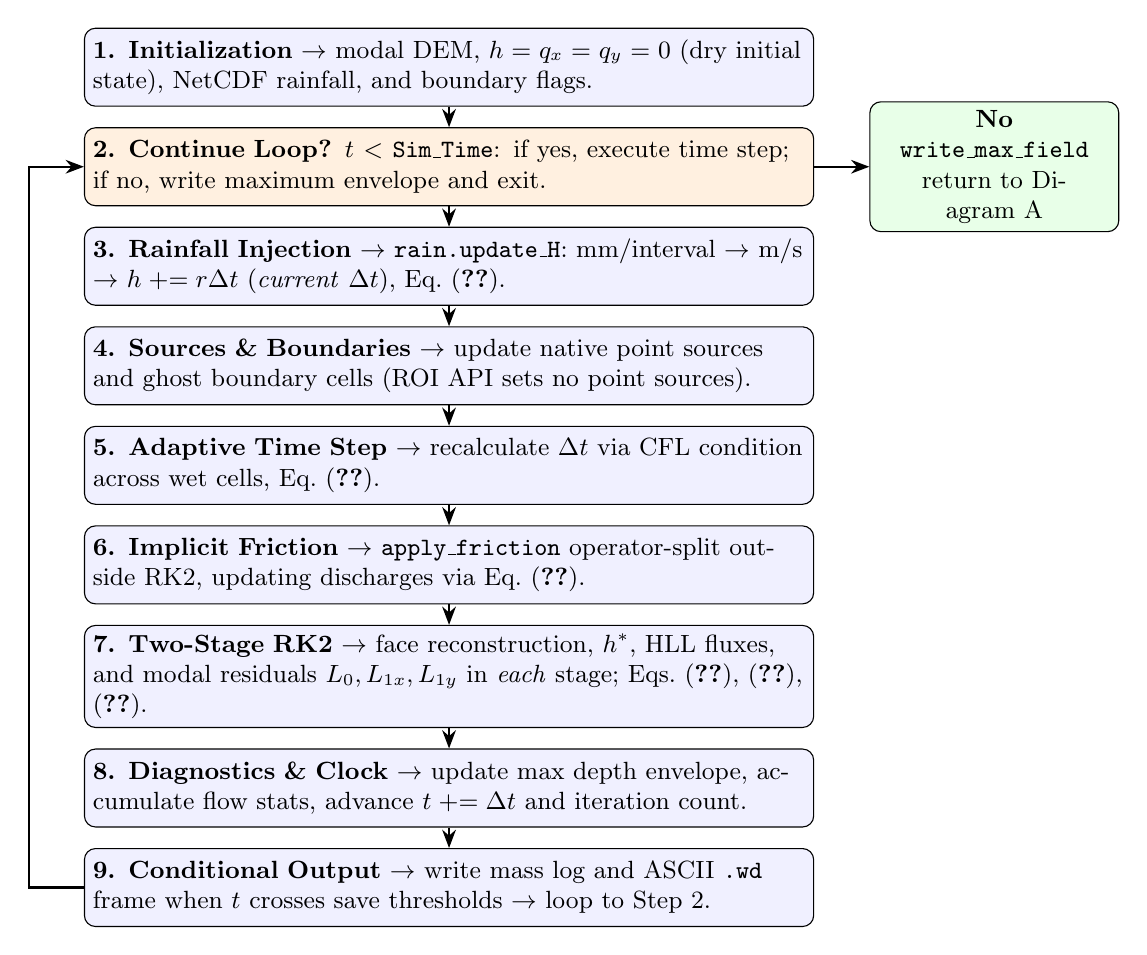
\begin{tikzpicture}[
 node distance=2.6mm,
 paso/.style={draw,rounded corners,fill=blue!6,align=left,text width=9.05cm,
              minimum height=.99cm,inner sep=3pt,font=\small},
 decision/.style={paso,fill=orange!12},
 final/.style={draw,rounded corners,fill=green!9,align=center,text width=2.95cm,
               inner sep=3pt,font=\small},
 flecha/.style={-{Stealth},thick}]
\node[paso] (b1) {\textbf{1. Initialization} $\to$ modal DEM, $h=q_x=q_y=0$ (dry initial state), NetCDF rainfall, and boundary flags.};
\node[decision,below=of b1] (b2) {\textbf{2. Continue Loop?} $t<\texttt{Sim\_Time}$: if yes, execute time step; if no, write maximum envelope and exit.};
\node[paso,below=of b2] (b3) {\textbf{3. Rainfall Injection} $\to$ \texttt{rain.update\_H}: mm/interval $\to$ m/s $\to$ $h\mathrel{+}=r\Delta t$ (\emph{current} $\Delta t$), Eq.~\eqref{eq:ncrain}.};
\node[paso,below=of b3] (b4) {\textbf{4. Sources \& Boundaries} $\to$ update native point sources and ghost boundary cells (ROI API sets no point sources).};
\node[paso,below=of b4] (b5) {\textbf{5. Adaptive Time Step} $\to$ recalculate $\Delta t$ via CFL condition across wet cells, Eq.~\eqref{eq:cfl}.};
\node[paso,below=of b5] (b6) {\textbf{6. Implicit Friction} $\to$ \texttt{apply\_friction} operator-split outside RK2, updating discharges via Eq.~\eqref{eq:fricdisc}.};
\node[paso,below=of b6] (b7) {\textbf{7. Two-Stage RK2} $\to$ face reconstruction, $h^*$, HLL fluxes, and modal residuals $L_0,L_{1x},L_{1y}$ in \emph{each} stage; Eqs.~\eqref{eq:weak}, \eqref{eq:hll}, \eqref{eq:rk}.};
\node[paso,below=of b7] (b8) {\textbf{8. Diagnostics \& Clock} $\to$ update max depth envelope, accumulate flow stats, advance $t\mathrel{+}=\Delta t$ and iteration count.};
\node[paso,below=of b8] (b9) {\textbf{9. Conditional Output} $\to$ write mass log and ASCII \texttt{.wd} frame when $t$ crosses save thresholds $\to$ loop to Step 2.};
\foreach \prim/\sig in {b1/b2,b2/b3,b3/b4,b4/b5,b5/b6,b6/b7,b7/b8,b8/b9}
  {\draw[flecha] (\prim.south)--(\sig.north);}
\node[final,right=7mm of b2] (fin) {\textbf{No}\\\texttt{write\_max\_field}\\return to Diagram A};
\draw[flecha] (b2.east)--(fin.west);
\draw[flecha] (b9.west)--++(-7mm,0) |- (b2.west);
\end{tikzpicture}
\end{center}
\noindent\textbf{Audit Anchors.} \texttt{rain.update\_H} in \src{rain/rain.tpp} executes prior to \texttt{Tstep\_from\_cfl}; \texttt{apply\_friction} executes prior to \texttt{rk\_stage1/2}. Each RK stage invokes \src{swe/dg2/modifiedvars.cpp} for hydrostatic face states, \src{swe/hll_include.h} for inter-cell fluxes, and \texttt{L0/L1x/L1y} in \src{swe/dg2.cpp} for the three modal amplitudes per field. Slope limiting is compiled in but \emph{disabled by default}; no infiltration routine is called in \texttt{dg2::solve}. Because frame output is checked after advancing $t$ without clamping $\Delta t$ to hit exact multiples of \texttt{saveint}, ASCII frame files do not record exact physical timestamps and the API explicitly reports \texttt{time\_s:null}.
\newpage
\noindent An authenticated \texttt{POST /api/flood-scenarios/roi/start/} validates in memory the JSON payload, polygon topology, metric CRS, theoretical NASADEM latitude bounds, and computational budgets before creating a run directory or initiating downloads. It accepts exactly seven top-level keys: \texttt{roi}, \texttt{domain}, \texttt{rainfall}, \texttt{rainfall\_profile}, \texttt{terrain}, \texttt{hydraulics}, and \texttt{simulation}. Server binary paths remain strictly server-controlled. A valid POST returns HTTP \texttt{202 Accepted} with a run UUID, \texttt{status\_url}, and \texttt{results\_url}, spawning an isolated background worker that atomically updates \texttt{state.json} and records SHA-256 hashes for all inputs, binaries, parameters, NetCDF forcing, and output COGs.

\begin{center}
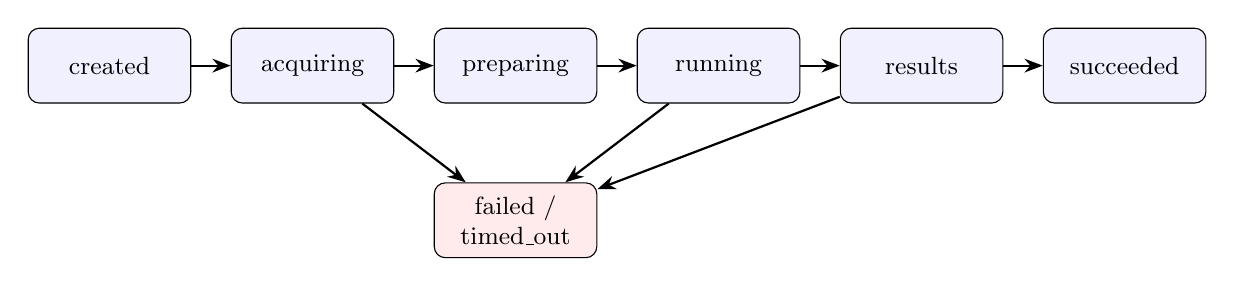
\begin{tikzpicture}[node distance=5mm and 5mm,box/.style={draw,rounded corners,fill=blue!6,align=center,text width=1.83cm,minimum height=.95cm,font=\small},bad/.style={box,fill=red!8},arr/.style={-{Stealth},thick}]
\node[box] (a) {created};\node[box,right=of a] (b) {acquiring};\node[box,right=of b] (c) {preparing};\node[box,right=of c] (d) {running};\node[box,right=of d] (e) {results};\node[box,right=of e] (f) {succeeded};
\foreach \u/\v in {a/b,b/c,c/d,d/e,e/f}{\draw[arr] (\u)--(\v);}
\node[bad,below=1cm of c] (g) {failed / timed\_out};
\draw[arr] (b)--(g);\draw[arr] (d)--(g);\draw[arr] (e)--(g);
\end{tikzpicture}
\end{center}
\noindent\texttt{GET /api/flood-roi-runs/<uuid>/} exposes live run state (returning sanitized error codes without internal stack traces or filesystem paths on failure). \texttt{GET .../results/} returns HTTP \texttt{409} until completion; upon \texttt{succeeded}, it returns grid metadata, metric CRS, units (\texttt{m above local bed}), ordered frame summaries, maximum envelope statistics, warnings, and artifact descriptors. \texttt{GET .../artifacts/<name>/} serves the verified \texttt{float32} COG TIFF exclusively to the authenticated run owner with an SHA-256 \texttt{ETag} (full download, no HTTP Range). Unauthorized or unknown UUIDs return HTTP \texttt{404} (see \src{backend/analyses/roi_flood_runs.py} and \src{docs/api-simulacion-roi.md}).

\subsection{Complete Illustrative Request Payload (Contract Example, Not a Calibrated Event)}
\begingroup\small
\begin{verbatim}
{
 "roi":{"type":"Polygon","coordinates":[[[-92.9998,16.8],[-92.9995,16.8],
 [-92.9995,16.8003],[-92.9998,16.8003],[-92.9998,16.8]]]},
 "domain":{"type":"Polygon","coordinates":[[[-92.9999,16.7998],
 [-92.9993,16.7998],[-92.9993,16.8005],[-92.9999,16.8005],
 [-92.9999,16.7998]]]},
 "rainfall":{"amount":2,"unit":"mm","duration":1,"duration_unit":"s"},
 "rainfall_profile":{"interval_count":2,"seed":7,
                     "distribution":"uniform_balanced"},
 "terrain":{"target_crs":"EPSG:32615","resolution_m":20,
            "resampling":"nearest"},
 "hydraulics":{"manning":0.02,"initial_condition":"dry_zero_velocity",
               "boundary":"free","infiltration":"unsupported",
               "domain_nonurban":true},
 "simulation":{"duration_s":2,"save_interval_s":1,"initial_tstep_s":0.1}
}
\end{verbatim}
\endgroup
All numbers in this payload illustrate the JSON schema and fast integration testing (2\,mm in 1\,s over a tiny domain followed by 1\,s of dry tail); they do not represent a realistic design storm or recommended hydraulic configuration.

\noindent\begin{tabularx}{\linewidth}{p{.23\linewidth}X}
\toprule API Field & Correct Technical Interpretation\\\midrule
\texttt{202 id/state/urls} & Confirms job admission only; does not imply solver completion or physical validity.\\
\src{frames[i].frame_index} & Sequential frame order. \texttt{time\_s:null} indicates that exact physical snapshot time is not stored in the native ASCII output. \texttt{scheduled\_time\_s=i*save\_interval\_s} is the requested save schedule, not an observed timestamp.\\
\texttt{maximum} & Cell-wise maximum water depth envelope across the simulation; does not correspond to a single instant in time.\\
\texttt{grid/nodata} & Metric CRS grid specification and sentinel value (\texttt{-9999}); NoData means unknown, never zero depth.\\
\texttt{artifacts} & Numerical \texttt{float32} COG TIFF in metric UTM CRS with SHA-256 hash and \texttt{EPSG:4326} bounding box for framing (not an RGB Web Mercator image or XYZ tile URL).\\
\src{synthetic:true}, \src{hydraulic_accuracy_validated:false} & Mandatory epistemic flags marking the run as an unvalidated synthetic scenario.\\\bottomrule
\end{tabularx}

\section{Service Parameters, Binary Traceability, and Error Handling}
\label{sec:operacion}
The generated \texttt{roi.par} file declares \texttt{dg2}, \src{DEMfile} \src{terrain.dem}, \texttt{sim\_time}, \texttt{saveint}, \src{initial_tstep}, \src{fpfric}, and \src{dynamicrainfile} \src{rain.nc} (plus \texttt{bcifile} when \texttt{boundary: "free"}). Both native binaries are verified against pinned server SHA-256 hashes prior to execution: solver binary \src{777d50f8d6a926260baa31b4c8ca3ecc0b3ae710494bebb2d4699ccf8c39775c} (LISFLOOD-FP 8.0 / 8.0.3 float CPU) and preprocessor \texttt{generateDG2DEM} \src{ada476fc141d536d09abd4aa1238d192bbddfd627574886ada12784ba0e964a8} (repository snapshot \src{615d0ce23eee51df7c130c93a1306958b2d0f0c6}).

\noindent\begin{tabularx}{\linewidth}{p{.28\linewidth}p{.15\linewidth}X}
\toprule Server Setting & Default & Operational Meaning and Constraint\\\midrule
\texttt{FLOOD\_ROI\_DG2\_ENABLED} & true & Setting \texttt{false} disables \texttt{roi/start/}; does not verify Earthdata credentials.\\
\texttt{MAX\_CELLS / MAX\_RAIN\_VALUES} & 1000 / 5000 & Initial computational grid and NetCDF array budgets.\\
\texttt{MAX\_FRAMES / MAX\_TILES} & 5 / 2 & Maximum saved output frames and intersecting NASADEM tiles per run.\\
\texttt{TIMEOUT\_S / PREPARATION\_TIMEOUT\_S} & 15 / 120\,s & Hard wall-clock timeouts for the solver process and preparation worker.\\\bottomrule
\end{tabularx}
Running \texttt{PYTHONPATH=. python backend/manage.py check\_flood\_service} verifies local binary hashes and offline readiness; passing \texttt{--earthdata} (operator-authorized) tests live NASADEM tile acquisition (\src{backend/config/flood_service.py}, \src{pipeline/hydrology/roi_runner.py}, \src{backend/analyses/roi_flood_runs.py}).

\section{Observed Verification Evidence and What It Does Not Prove}
\label{sec:evidencia}
Two distinct verification artifacts are recorded in the repository and must never be conflated into a claim of regional flood validation:
\begin{enumerate}
\item \textbf{End-to-end solver integration with synthetic HGT tiles:} completed with status \texttt{succeeded} on a $9\times8$ grid at 20\,m resolution, producing three \texttt{.wd} frames, one maximum envelope, and four \texttt{EPSG:32615} COGs (\src{data/test-runs/roi-dg2-136934da-7370-4113-b337-36ebc0bcafcc/6c5b38f4-9d14-4c71-912b-04ed7629d94a/state.json}). This proves adapter--solver pipeline continuity, not real-world hydraulic accuracy.
\item \textbf{Live Earthdata NASADEM granule acquisition check:} independently verified download of tile \texttt{n16w094} ($14,251,621$-byte ZIP, \src{data/service-checks/7507c3c0-8ba1-43b1-920e-a35fa58ea70f/proof.json}).
\end{enumerate}
\begin{tabularx}{\linewidth}{p{.23\linewidth}p{.37\linewidth}X}
\toprule Verification Tier & Available Evidence & Remaining Scientific Requirements\\\midrule
Format \& Integration & Manifests, SHA-256 hashes, native NetCDF, synthetic-seam ASCII/COG outputs. & Per-case input/output auditing before scaling to larger regional domains.\\
Numerical Mathematics & Operator equations and dimensional consistency documented herein. & Automated lake-at-rest, variable-bed, wet--dry front, and grid/time convergence benchmarks.\\
Volumetric Mass Balance & Rainfall forcing log and native \texttt{.mass} diagnostic file. & Audit \texttt{Qerror/Verror} and verify $V_f-V_i$ against boundary outflows within pre-declared tolerances.\\
Physical Fidelity & No regional flood event validated in these integration tests. & Catchment delineation, channel bathymetry, gauge/rain observations, spatially distributed Manning $n_M$, infiltration, and independent satellite/field validation.\\\bottomrule
\end{tabularx}

\section{Equation-to-Code Audit Map}
\label{sec:mapa}
In the table below, native C++ paths are relative to \src{data/tools/lisflood-fp-8.0/runtime/source/}:
\begin{longtable}{p{.19\linewidth}p{.34\linewidth}p{.38\linewidth}}
\toprule Equation \& SI Unit & Source Function \& Output & Audit \& Interpretation Control\\\midrule\endhead
\eqref{eq:conserv}--\eqref{eq:flux}, m/s \& m$^2$/s$^2$ & \src{swe/flux.cpp}: \texttt{physical\_flux\_x/y}; \src{swe/dg2.cpp}: \texttt{L0/L1x/L1y} & Distinguish cell-mean residual from linear slope modes; spatial derivatives divide by meters.\\
\eqref{eq:vertices}, m & \src{preprocess/generateDG2DEM.cpp} \& \src{swe/dg2/fields.cpp}: \texttt{.dem/.dem1x/.dem1y} & Modal slope amplitudes carry units of meters (EGM96), not dimensionless GIS slope m/m.\\
$z^*,h^*,q^*$, m, m, m$^2$/s & \src{swe/dg2/modifiedvars.cpp}: \texttt{initialise\_Zstar}, \texttt{update\_Hstar}, \texttt{discharge\_star} & Hydrostatic face reconstruction prevents uphill flux at wet--dry edges.\\
\eqref{eq:hll}, m$^2$/s \& m$^3$/s$^2$ & \src{swe/hll_include.h}: intermediate fan; \src{swe/dg2.cpp}: \texttt{update\_fluxes} & Transverse momentum uses contact-wave upwinding rather than component-wise HLL.\\
\eqref{eq:fricdisc}, m$^2$/s & \src{swe/dg2/friction.cpp}: \texttt{friction}, \texttt{apply\_friction} & Separate dimensionless energy slope $S_f$ from momentum source $-C_fuw$; split outside RK2.\\
\eqref{eq:cfl}, s; \eqref{eq:rk}, units of $U$ & \src{swe/dg2.cpp}: \texttt{min\_dt}, \texttt{rk\_stage1/2}, \texttt{solve} & Adaptive CFL step does not clamp to exact \texttt{saveint} multiples.\\
\eqref{eq:rainbal}--\eqref{eq:ncrain}, m \& m/s & \src{pipeline/hydrology/rainfall.py}, \src{pipeline/hydrology/rainfall_netcdf.py}, \src{rain/rain.tpp} & Distinguish mm/interval in NetCDF, hours on time axis, and m/s inside solver loop.\\
Water depth $h$, m above bed & \src{pipeline/hydrology/results.py}: \texttt{summarize\_results}, \texttt{export\_depth\_cog} & NoData is unknown (not dry bed); numerical COG is in metric UTM CRS.\\\bottomrule
\end{longtable}

\section{Interpretation Limits and Prerequisites for a Scientific Case Study}
\label{sec:limites}
Before interpreting a simulation as a real-world hydrological study, the analyst must establish: the physical storm event, the full contributing watershed domain, the UTC time origin, DEM vertical accuracy and channel bathymetry, initial wetness and river baseflow, physically justified boundary conditions, representative spatio-temporal rainfall, infiltration losses (currently unsupported in the ROI path), spatially distributed Manning roughness, and exclusion of unmodeled urban drainage networks. Furthermore, satellite flood observations represent single-instant snapshots and must be compared against corresponding simulation times (accounting for timestamp uncertainty) rather than against the asynchronous multi-hour maximum envelope.

\section{How to Read and Use Simulation Outputs}
\label{sec:leer-resultados}

This section translates the API response schema into practical guidelines for reading downloaded flood simulation outputs.

\subsection{Water Depth $h$: ``Meters Above Local Bed''}

Reported depth values measure water thickness in meters \emph{above the local DEM cell bed}, not absolute elevation above sea level:
\begin{itemize}
  \item A value of $h = 0.30$\,m means a 30\,cm water column sitting on top of that cell's DEM elevation $z_b$. The absolute water-surface elevation is $\eta = z_b + h$.
  \item Comparing $\eta$ against external river-gauge stages requires verifying that both share the same vertical datum (NASADEM uses the EGM96 geoid).
\end{itemize}

\subsection{Time Frames vs.\ Maximum Depth Envelope}

\begin{description}[style=nextline]
  \item[Scheduled Frames (\texttt{frames}).] Each frame captures the spatial depth field after the solver clock crosses a multiple of \texttt{save\_interval\_s}. While \texttt{frame\_index} order is exact, the native ASCII output does not record the exact floating-point physical second at which the frame was written, so the API reports \texttt{time\_s: null} alongside \texttt{scheduled\_time\_s}.
  \item[Maximum Envelope (\texttt{maximum}).] The cell-by-cell peak water depth reached at any point during the entire simulation. It is a temporal envelope rather than a simultaneous snapshot: different cells reach their peak depth at different times.
\end{description}

\begin{cuidado}
Comparing the simulation's \emph{maximum temporal envelope} against a single-pass \emph{satellite snapshot} compares two different physical quantities. An instantaneous observation at time $t_{\text{obs}}$ should be compared against the frame closest to $t_{\text{obs}}$, explicitly noting any temporal offset.
\end{cuidado}

\subsection{NoData vs.\ Wet Cells}

The sentinel value \texttt{nodata} (\texttt{-9999}) marks cells without valid computation; it means \emph{unknown}, never ``zero water depth''. Conversely, the summary statistic \texttt{wet\_cells} counts all valid cells with $h > 0$ (even microscopic films of $10^{-6}$\,m) and must not be reported as ``inundated hazard area'' without applying a physically motivated depth threshold (e.g., $h \ge 0.05$\,m or $0.10$\,m).

\subsection{Using Metric COGs in a Web Map}

Downloaded artifacts are single-band \texttt{float32} Cloud-Optimized GeoTIFFs (COGs) in the requested metric UTM CRS. They are raw numerical rasters, not pre-colored RGB Web Mercator tiles; rendering them on a MapLibre GL canvas requires explicit reprojection and colormap application.

\subsection{Mandatory Epistemic Flags}

Every successful response permanently carries \texttt{synthetic: true} and \texttt{hydraulic\_accuracy\_validated: false}, reminding consumers that the output belongs to the \emph{prediction / scenario} tier (Section~\ref{sec:tres-niveles}).

\subsection{From ``Technically Functional'' to ``Scientifically Defensible''}

Table~\ref{tab:de-tecnico-a-cientifico} summarizes the scientific steps required to elevate an exploratory run into a defensible hydrological study.

\begin{table}[htbp]
\centering\small
\begin{tabularx}{\linewidth}{p{.27\linewidth}X}
\toprule
\textbf{Scientific Task} & \textbf{Why It Is Required}\\\midrule
Delineate the contributing watershed & A small visual ROI rarely contains the upslope catchment feeding runoff.\\
Prescribe physical boundary conditions & Idealized \texttt{free} or \texttt{closed} box edges can artificially drain or pond water.\\
Calibrate/justify Manning $n_M$ & Roughness controls flow speed, peak attenuation, and arrival times.\\
Account for soil infiltration & Without infiltration, 100\,\% of rainfall becomes surface runoff.\\
Audit volumetric mass conservation & Verify that final stored volume equals cumulative rainfall minus boundary outflow within pre-declared tolerances.\\
Run classical numerical benchmarks & Lake-at-rest, Ritter dam-break, wet--dry front tracking, and mesh convergence.\\
Validate against independent observations & Without external gauge, field, or optical/SAR validation, results remain exploratory.\\\bottomrule
\end{tabularx}
\caption{Requirements to move from a technically verified run to a scientifically defensible flood study.}
\label{tab:de-tecnico-a-cientifico}
\end{table}

\begin{intuicion}
An unvalidated simulation is still highly valuable: it allows analysts to explore topographic drainage pathways, test sensitivity to rainfall intensity, and identify depressions prone to ponding. Maintaining a clear boundary between scenario exploration and validated forecasting allows users to leverage the tool without overclaiming certainty.
\end{intuicion}


\section{How to Verify a Hydrodynamic Flood Simulator}
\label{sec:verificacion}

A numerical solver always outputs numbers, whether physically sound or not. A plausible-looking depth map proves nothing by itself: a sign error in a bed-slope source term can still produce smooth-looking water puddles. Standard scientific computing practice therefore separates \emph{verification} (does the code solve its governing equations accurately?) from \emph{validation} (do those equations with these inputs accurately represent a real-world flood?). This section outlines five standard verification benchmarks.

\begin{atencion}
Verification is not validation. A verified solver accurately integrates the 2D Shallow Water Equations; however, if the input DEM lacks river channel bathymetry or the rainfall scenario is hypothetical, the output remains an exploratory scenario rather than an observed truth.
\end{atencion}

\subsection{Test 1: Lake at Rest (Well-Balanced Property)}

\paragraph{Setup.} Take an irregular, bumpy bed topography $z_b(x,y)$ and partially fill it with stationary water ($u=v=0$) up to a flat horizontal free surface $\eta = h + z_b = \text{constant}$, with zero rainfall, zero friction, and closed boundaries. The exact analytical solution is that \emph{the water remains completely motionless forever}.

\paragraph{What It Verifies.} It tests the \emph{well-balanced} property ($C$-property). In the momentum equation, the hydrostatic pressure gradient $\tfrac12 g\,\partial_x(h^2)$ must balance the bed-slope source term $-gh\,\partial_xz_b$ to machine precision. If their discrete approximations are mismatched, the solver generates spurious numerical currents crawling up and down submerged bumps. Hydrostatic reconstruction (Section~\ref{sec:dg2}) is specifically designed to enforce this exact cancellation.

\paragraph{Acceptance Criterion.} Maximum spurious velocity after thousands of time steps must remain near floating-point roundoff ($\lesssim 10^{-10}$\,m/s in double precision, or $\lesssim 10^{-6}$\,m/s in single precision), never on the order of $10^{-2}$\,m/s.

\begin{ejemplo}[How Small Is ``Zero''?]
If after 10,000 steps the maximum velocity is $3\times10^{-13}$\,m/s, the scheme is well-balanced. If it is $4\times10^{-3}$\,m/s, the scheme fails: sustained over 24 hours, a $4$\,mm/s parasitic current would displace water by $\approx350$\,m in the absence of any physical forcing.
\end{ejemplo}

\subsection{Test 2: Ritter's Analytical Dam-Break Solution}

Comparing numerical output against Ritter's exact 1D frictionless dam-break solution (Equation~\eqref{eq:ritter}, derived in Section~\ref{sec:der-swe}) tests shock-capturing and wet--dry front propagation simultaneously across three regimes: an initial discontinuity, a rarefaction fan, and a wet--dry shoreline advancing over a dry flat bed.

\paragraph{Procedure.}
\begin{enumerate}
  \item Initialize $h(x,0)=h_0$ for $x<0$ and $h(x,0)=0$ for $x>0$ over a flat frictionless bed ($z_b=0$, $n_M=0$, $r=0$).
  \item Integrate to time $T$ (e.g., $T=6$\,s) and extract cell-center depths $h_i^{\text{num}}$.
  \item Evaluate the $L_1$ error norm against Ritter's exact solution $h(x_i,T)$:
        \[
          E=\frac{1}{N}\sum_{i=1}^{N}\bigl|h_i^{\text{num}}-h(x_i,T)\bigr| .
        \]
  \item Repeat across progressively refined grids $\Delta x$ to measure the empirical convergence rate (Test 4).
\end{enumerate}

\paragraph{Expected Behavior.} While a second-order scheme slightly smears the slope corners across a few cells, the wet--dry tip must track $x_f=2c_0T$ ($c_0=\sqrt{gh_0}$) without systematic phase lag or negative depths.

\subsection{Test 3: Global Volumetric Mass Conservation}

Because the solver integrates a conservation law, total stored water volume $V^n=\sum_K h_K^n\,A_K$ must change solely due to surface rainfall minus net boundary outflow:
\begin{equation}
  V^{n+1}-V^{n}=\Delta t\,\Bigl(\underbrace{\sum_K r_K A_K}_{\text{rainfall inflow}}
  -\underbrace{\sum_{\text{boundaries}}\textstyle\int q_n\,\dd\ell}_{\text{net boundary outflow}}\Bigr).
  \label{eq:balance}
\end{equation}
All internal face fluxes cancel pairwise because the numerical flux exiting cell $K$ across an interior face equals the flux entering its neighbor. Any violation beyond floating-point precision (or documented wet--dry cutoff tolerances) indicates a conservation bug.

\begin{ejemplo}[Closed-Basin Rainfall Volume Balance]
A $4\ \mathrm{km}^2$ domain with closed (\texttt{NONE}) boundaries receives $60$\,mm of total rainfall. The final water volume stored in the domain must equal $60\times10^{-3}\ \mathrm{m}\times4\times10^{6}\ \mathrm{m}^2=2.4\times10^{5}\ \mathrm{m}^3$ ($24\ \mathrm{m}^3$ per $20\times20$\,m cell).
\end{ejemplo}

\subsection{Test 4: Empirical Order of Convergence}

For a scheme of formal accuracy order $p$, the global error norm scales as $E\propto\Delta x^{p}$. Given errors $E_1$ and $E_2$ measured on two grids of spacing $\Delta x_1>\Delta x_2$, the observed order of convergence is:
\begin{equation}
  p_{\text{obs}}=\frac{\ln(E_1/E_2)}{\ln(\Delta x_1/\Delta x_2)} .
  \label{eq:orden}
\end{equation}

\begin{ejemplo}[Illustrative Convergence Rate Calculation]
Suppose a smooth wave benchmark yields $E_1=0.040$\,m at $\Delta x_1=10$\,m and $E_2=0.011$\,m at $\Delta x_2=5$\,m. Then
$p_{\text{obs}}=\ln(0.040/0.011)/\ln2=\ln(3.64)/0.693=1.86$,
confirming near-second-order behavior on smooth flows (illustrative numbers).
\end{ejemplo}

\begin{cuidado}
Across sharp discontinuities or wet--dry fronts, the observed $L_1$ convergence order naturally degrades toward $p_{\text{obs}} \approx 1$. Smooth wave benchmarks measure formal polynomial accuracy order, whereas dam-break benchmarks test shock-capturing robustness.
\end{cuidado}

\subsection{Test 5: Physical Parameter Sensitivity}

When no closed-form analytical solution exists (e.g., over real DEM topography), qualitative sensitivity checks verify that the solver responds to parameter perturbations in the physically expected direction (Table~\ref{tab:sensibilidad}).

\begin{table}[htbp]
\centering
\caption{Expected qualitative physical sensitivities of the flood simulator.}
\label{tab:sensibilidad}
\small
\begin{tabularx}{\linewidth}{@{}lXX@{}}
\toprule
Input Perturbation & Expected Physical Response & Red-Flag Anomaly \\
\midrule
Double rainfall depth & Larger total volume and higher peak depths (nonlinearly) & Peak depth decreases \\
Increase Manning $n_M$ & Slower flow velocities; delayed and locally deeper ponding & Faster wave propagation \\
Refine grid resolution $\Delta x$ & Sharper wet--dry fronts; stable domain-integrated volume & Large shift in total water volume \\
Reduce CFL number & Virtually identical depth solution & Solution changes substantially \\
Smooth bed topography & Less localized depression ponding & Increased localized trapping \\
\bottomrule
\end{tabularx}
\end{table}

\subsection{Verification Test Log Template}

To keep verification auditable, every benchmark run should be recorded using a standardized template (Table~\ref{tab:registro}) with pass/fail acceptance thresholds declared \emph{prior} to execution.

\begin{table}[htbp]
\centering
\caption{Standardized verification test record template.}
\label{tab:registro}
\small
\begin{tabularx}{\linewidth}{@{}lX@{}}
\toprule
Field & Content \\
\midrule
Test ID & Short benchmark identifier and execution date \\
Code Version & Git commit hash and binary SHA-256 \\
Grid Specification & $\Delta x$, total cells, metric CRS \\
Physical Parameters & Manning $n_M$, rainfall forcing, CFL number, simulated duration $T$ \\
Error Metric & $L_1$ error $E$, maximum spurious speed, or mass-balance residual \\
Acceptance Criterion & Threshold fixed \emph{before} running the test \\
Result \& Verdict & Measured metric value and Pass / Fail status \\
Notes & Any wet--dry depth cutoffs or boundary warnings observed \\
\bottomrule
\end{tabularx}
\end{table}


\section{References and Version Provenance for Part~\ref{part:inundacion}}
\begin{enumerate}
\item Shaw, J., Kesserwani, G., Neal, J., Bates, P., \& Sharifian, M.~K. (2021). ``LISFLOOD-FP 8.0: the new discontinuous Galerkin shallow-water solver for multi-core CPUs and GPUs'', \emph{Geoscientific Model Development}, 14, 3577--3602. \url{https://doi.org/10.5194/gmd-14-3577-2021}.
\item LISFLOOD-FP 8.0 official Zenodo archive: \url{https://zenodo.org/records/4073011}; developer execution guide: \url{https://www.seamlesswave.com/LISFLOOD8.0}. All discrete operator equations documented above were audited directly against the local C++ source tree under \src{data/tools/lisflood-fp-8.0/runtime/source/}.
\item NASA LP DAAC (2025). \emph{NASADEM User Guide, Version 1.3} (\texttt{NASADEM\_HGT v001}, EGM96 vertical datum): \url{https://lpdaac.usgs.gov/documents/2237/NASADEM_User_Guide_V13.pdf}.
\item Repository contracts and implementation specs: \src{docs/api-simulacion-roi.md}, \src{docs/configuracion-servicio-inundacion.md}, \src{docs/distribucion-lluvia.md}, \src{docs/dem-dg2.md}, \src{docs/resultados-dg2.md}, and source files mapped in Section~\ref{sec:mapa}.
\end{enumerate}

\clearpage

\part{Terrain Solar Irradiance}
\label{part:solar}

\section{Scope of the Solar Irradiance Simulator}
\label{sec:solar-alcance}

This part documents the behavior implemented in \src{pipeline/solar/*.py} and
\src{backend/solar/*.py}. The execution pipeline follows six sequential steps:
\begin{enumerate}
  \item resolves local timestamp, IANA time zone, and atmospheric state;
  \item prepares a metric-grid DEM from \texttt{NASADEM\_HGT v001};
  \item computes high-precision solar position via the NREL SPA algorithm;
  \item estimates clear-sky Direct Normal Irradiance (DNI) using the pvlib Ineichen--Perez formulation;
  \item derives local topographic surface normals from the metric DEM;
  \item projects the adjusted direct beam irradiance onto each terrain facet.
\end{enumerate}
The output is an instantaneous climatological model of incident direct solar irradiance, in
W\,m$^{-2}$, rather than an in-situ pyranometer measurement or locally validated weather forecast. Invalid or masked pixels are preserved as NoData.

\noindent\textbf{What Is Not Computed.} The simulator does not model material absorption, surface albedo reflection, transmittance, diffuse sky irradiance, or cloud cover. (Detailed API contracts and discrete equations are also covered in Section~\ref{sec:solar-api-arch}).

\section{Conceptual Foundations of Direct Solar Irradiance on Terrain}
\label{sec:solar-fundamentos}

\begin{atencion}
This section and the next explain the \emph{fundamental radiative and geometric physics} underlying the solar pipeline. They provide conceptual clarity for interpreting the outputs, while the exact API implementation and parameter contracts follow Section~\ref{sec:solar-alcance} and Section~\ref{sec:solar-api-arch}.
\end{atencion}

\subsection{Four Questions, Four Stages}

The solar simulator answers four independent physical questions in strict sequence:
\begin{enumerate}
  \item \textbf{Where is the Sun in the sky at this instant?} Spherical astronomy as a function of geographic coordinates and UTC time.
  \item \textbf{How much direct solar beam power survives a clear atmosphere?} Atmospheric extinction yielding Direct Normal Irradiance (DNI).
  \item \textbf{How is the terrain tilted at each pixel?} Differential geometry of the Digital Elevation Model (surface normal vector).
  \item \textbf{How much direct beam power strikes that tilted facet per unit area?} The dot-product projection of the first three answers.
\end{enumerate}

\begin{figure}[htbp]
\centering
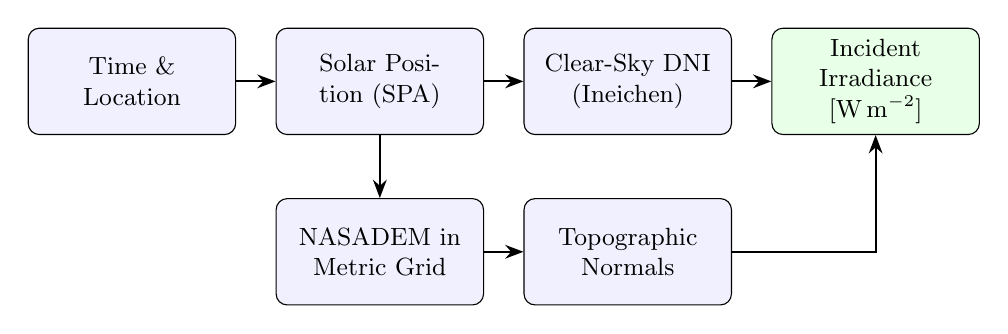
\begin{tikzpicture}[node distance=5mm,
  caja/.style={draw,rounded corners,fill=blue!6,align=center,text width=2.4cm,minimum height=1.35cm,font=\small},
  sal/.style={caja,fill=green!9},
  fl/.style={-{Stealth},thick}]
\node[caja] (a) {Time \& Location};
\node[caja,right=of a] (b) {Solar Position (SPA)};
\node[caja,right=of b] (c) {Clear-Sky DNI (Ineichen)};
\node[caja,below=8mm of b] (d) {NASADEM in Metric Grid};
\node[caja,right=of d] (e) {Topographic Normals};
\node[sal,right=of c] (f) {Incident Irradiance [W\,m$^{-2}$]};
\draw[fl] (a)--(b); \draw[fl] (b)--(c); \draw[fl] (c)--(f);
\draw[fl] (d)--(e); \draw[fl] (e.east) -| (f.south);
\draw[fl] (b.south) -- (d.north);
\end{tikzpicture}
\caption{Conceptual stages of the solar irradiance pipeline. The final projection combines the solar unit vector, clear-sky DNI, and the DEM surface normal.}
\label{fig:cadena-solar}
\end{figure}

\subsection{Solar Position}

The apparent position of the Sun in the local sky is specified by two angles: the \textbf{solar zenith angle} $\theta_z$ (measured from the local vertical; $0^\circ$ is the Sun directly overhead at zenith) and the \textbf{solar azimuth} $\phi_s$ (horizontal compass bearing, measured clockwise from North toward East). The \textbf{solar elevation} $e$ is the complement of the zenith angle, $e = 90^\circ-\theta_z$. To first order, the cosine of the zenith angle depends on observer latitude $\varphi$, solar declination $\delta$ (the latitude at which the Sun is overhead at solar noon on that day of the year), and hour angle $\omega$ (angular rotation of the Earth since local solar noon, $15^\circ$ per hour):
\begin{equation}
  \cos\theta_z=\sin\varphi\sin\delta+\cos\varphi\cos\delta\cos\omega .
  \label{eq:cenit}
\end{equation}
High-precision ephemeris algorithms such as NREL's SPA (\emph{Solar Position Algorithm}, Reda \& Andreas, 2004) additionally account for Earth's orbital eccentricity, axial nutation, atmospheric refraction (dependent on local barometric pressure and temperature), and the equation of time. SPA achieves an angular uncertainty of $\sim 0.0003^\circ$, far smaller than DEM slope or atmospheric turbidity uncertainties.

\subsection{Clear-Sky Direct Normal Irradiance (DNI)}

\textbf{DNI} is the solar beam power per unit area arriving directly from the solar disk onto a surface oriented perpendicular to the sunbeams. At the top of the atmosphere, this equals the extraterrestrial solar irradiance $I_0$ ($\approx 1361$\,W\,m$^{-2}$, modulated by $\pm 3.3\,\%$ over the year due to Earth--Sun distance). Passing through the atmosphere, a fraction is absorbed and scattered; what remains in the direct beam is DNI. A standard clear-sky functional form of the Ineichen--Perez type is:
\begin{equation}
  \mathrm{DNI}\approx I_0\,b\,\exp\!\bigl[-0.09\,m\,(T_L-1)\bigr],
  \label{eq:dni}
\end{equation}
where $m$ is relative optical air mass, $T_L$ is the \textbf{Linke turbidity factor}, and $b$ is an altitude-dependent coefficient:
\begin{itemize}
  \item \textbf{Optical Air Mass $m$} measures how many vertical atmosphere thicknesses the slanting sunbeam traverses. It equals $1$ when the Sun is at zenith ($\theta_z=0^\circ$) and grows roughly as $1/\cos\theta_z$ (regularized near the horizon by the Kasten--Young formula, yielding $m\approx 2.0$ at $\theta_z=60^\circ$).
  \item \textbf{Linke Turbidity $T_L$} expresses the optical thickness of the aerosol- and water-vapor-laden atmosphere as the equivalent number of clean, dry Rayleigh atmospheres producing the same attenuation. Low values ($T_L \approx 2$--$3$) represent very clear skies; higher values ($T_L \ge 5$) represent humid or hazy tropical air masses.
\end{itemize}
Equation~\eqref{eq:dni} is a Beer--Lambert exponential attenuation law in which optical depth scales with $m(T_L-1)$.

\figura{sol_dni_aire}{0.66}{Clear-sky DNI structure (as a fraction of extraterrestrial $I_0$ at sea level) vs.\ solar zenith angle $\theta_z$ for four Linke turbidity values $T_L$.}

\begin{cuidado}
Equation~\eqref{eq:dni} models a cloud-free \emph{climatological} atmosphere. A clear-sky DNI value represents a physical upper envelope for direct beam irradiance at that location and timestamp under sunny conditions, never a reconstruction of actual historical cloud cover.
\end{cuidado}

\subsection{Topographic Surface Normals from a DEM}

A metric DEM provides elevation $z(x,y)$ on a planar grid. Local terrain gradients $\partial z/\partial x$ (East--West) and $\partial z/\partial y$ (North--South) are estimated via finite differences across neighboring cells. The upward-pointing unit surface normal vector to $z(x,y)$ is:
\begin{equation}
  \hat{\mathbf{n}}=\frac{\bigl(-\partial_xz,\ -\partial_yz,\ 1\bigr)}{\sqrt{1+(\partial_xz)^2+(\partial_yz)^2}},
  \label{eq:normal}
\end{equation}
where $x$ points East, $y$ points North, and the third component points toward the local zenith. The \textbf{slope angle} $\beta$ is the tilt between $\hat{\mathbf{n}}$ and the vertical ($\tan\beta=\sqrt{(\partial_xz)^2+(\partial_yz)^2}$), and the \textbf{aspect} $\phi_n$ is the horizontal compass direction the slope faces.

Because gradients are evaluated at the DEM grid spacing ($\approx 30$\,m for native NASADEM), micro-relief finer than the cell size is smoothed out.

\subsection{Projecting DNI onto the Tilted Surface}

Letting $\hat{\mathbf{s}}=(\cos e\,\sin\phi_s,\ \cos e\,\cos\phi_s,\ \sin e)$ denote the unit vector pointing from the ground facet toward the Sun (at elevation $e = 90^\circ-\theta_z$), the direct beam irradiance incident on a surface with unit normal $\hat{\mathbf{n}}$ is:
\begin{equation}
  I_{\mathrm{dir}}=\mathrm{DNI}\ \max\!\bigl(0,\ \hat{\mathbf{n}}\!\cdot\!\hat{\mathbf{s}}\bigr),
  \qquad
  \hat{\mathbf{n}}\!\cdot\!\hat{\mathbf{s}}=\cos\theta_z\cos\beta+\sin\theta_z\sin\beta\cos(\phi_s-\phi_n),
  \label{eq:proyeccion}
\end{equation}
where $\phi_n$ is the slope aspect. The dot product $\hat{\mathbf{n}}\!\cdot\!\hat{\mathbf{s}} = \cos\theta$ equals the cosine of the local solar incidence angle $\theta$ between the sunbeam and the facet normal (Figure~\ref{fig:sol_geometria}); clamping at zero accounts for self-shadowing when the Sun lies behind the slope ($\theta \ge 90^\circ$).

\figura{sol_geometria}{0.62}{The incidence angle $\theta$ between facet normal $\hat{\mathbf{n}}$ and solar vector $\hat{\mathbf{s}}$ determines the projected DNI fraction $\cos\theta$. Shown: slope $\beta=25^\circ$, solar zenith $\theta_z=40^\circ$, and a slope facing away from the Sun ($\theta=65^\circ$).}

\begin{ejemplo}[A $25^\circ$ Slope with the Sun at $40^\circ$ Elevation]
With $\theta_z=50^\circ$ (solar elevation $40^\circ$), slope $\beta=25^\circ$, and $\mathrm{DNI}=800$\,W\,m$^{-2}$ (illustrative), the geometric projection factor depends strongly on slope aspect relative to the Sun:
\begin{center}\small
\begin{tabular}{lccc}
\toprule
Slope Orientation Relative to Sun & $\hat{\mathbf{n}}\!\cdot\!\hat{\mathbf{s}}$ & Incident Direct Irradiance & Ratio vs.\ Flat Ground\\\midrule
Horizontal ground ($\beta=0^\circ$) & $0.643$ & $514$\,W\,m$^{-2}$ & $1.00$\\
Sun-facing slope ($\phi_s-\phi_n=0^\circ$) & $0.906$ & $725$\,W\,m$^{-2}$ & $1.41$\\
Cross-slope ($90^\circ$) & $0.583$ & $466$\,W\,m$^{-2}$ & $0.91$\\
Back-facing slope ($180^\circ$) & $0.259$ & $207$\,W\,m$^{-2}$ & $0.40$\\\bottomrule
\end{tabular}
\end{center}
For flat ground, $\hat{\mathbf{n}}\!\cdot\!\hat{\mathbf{s}} = \cos 50^\circ = 0.643$; for the sun-facing slope, the surface normal tilts $25^\circ$ toward the Sun, reducing the incidence angle to $50^\circ-25^\circ=25^\circ$ ($\cos 25^\circ = 0.906$). Thus, a $25^\circ$ sun-facing slope intercepts $41\,\mathrm{\%}$ more direct beam power per square meter than flat terrain, whereas the opposite slope receives $60\,\mathrm{\%}$ less.
\end{ejemplo}

\figura{sol_cos_pendiente}{0.66}{Projected DNI fraction $\max(0,\cos\theta)$ vs.\ terrain slope $\beta$ at solar zenith $\theta_z=50^\circ$ for three slope orientations. A sun-facing slope gains irradiance until its normal aligns with the sunbeam ($\beta=50^\circ$); a back-facing slope loses irradiance until reaching self-shadowing cutoff at $\beta=40^\circ$.}

\subsection{From a Single Facet to a Pixel-by-Pixel Map}

Evaluating Equation~\eqref{eq:proyeccion} across every cell of a DEM produces a spatial irradiance field. Figure~\ref{fig:sol_terreno} illustrates this over a \emph{synthetic} two-hill surface with the Sun in the Southeast ($\phi_s=135^\circ$) at $40^\circ$ elevation: Southeast-facing slopes appear bright ($\cos\theta / \cos\theta_z > 1$), whereas Northwest-facing back-slopes appear dark.

\figura{sol_terreno}{1.0}{Synthetic two-hill topography (left) and geometric projection ratio $\max(0,\hat{\mathbf{n}}\!\cdot\!\hat{\mathbf{s}})/\cos\theta_z$ relative to flat terrain (right), with the Sun at azimuth $135^\circ$ (SE) and $40^\circ$ elevation (20\,m grid).}

\subsection{Unmodeled Effects and Direction of Bias}

Understanding which physical processes are omitted tells the analyst the exact sign of potential bias:
\begin{description}[style=nextline]
  \item[Cast horizon shadows from distant ridges.] A valley cell may face toward the Sun locally ($\hat{\mathbf{n}}\!\cdot\!\hat{\mathbf{s}} > 0$) while being blocked by a tall mountain ridge upwind along the sunbeam. When cast shadows are omitted at low solar elevations, valley irradiance is \emph{overestimated}.
  \item[Diffuse sky radiation.] Rayleigh and aerosol scattering illuminate shaded slopes even when direct beam incidence is zero. Omitting diffuse irradiance \emph{underestimates} total global tilted irradiance (GTI) on shaded slopes.
  \item[Terrain-reflected irradiance (albedo).] Adjacent sunlit slopes reflect a small fraction of radiation onto facing valley walls.
  \item[Material absorption vs.\ incident flux.] The output reports incident radiative flux (W\,m$^{-2}$) arriving at the surface boundary, not net absorbed thermal energy.
  \item[Cloud cover.] Clear-sky atmospheric modeling provides a sunny-day baseline.
\end{description}

\subsection{How to Read the Solar Output}

\begin{itemize}
  \item \textbf{Instantaneous power flux:} Values are reported in W\,m$^{-2}$ at the requested timestamp (not daily integrated energy in W\,h\,m$^{-2}$).
  \item \textbf{Strict NoData preservation:} Masked pixels outside the ROI remain NoData rather than zero ($0$\,W\,m$^{-2}$ represents a valid dark or nighttime facet).
  \item \textbf{Climatological baseline:} The output should be interpreted as clear-sky direct beam potential controlled by topographic orientation.
\end{itemize}

\begin{table}[htbp]
\centering\small
\begin{tabularx}{\linewidth}{p{.28\linewidth}p{.18\linewidth}X}
\toprule
\textbf{Unmodeled Factor} & \textbf{Bias Direction} & \textbf{Where It Matters Most}\\\midrule
Distant ridge cast shadows & Overestimates & Deep valleys and canyons at low solar elevation.\\
Omitted diffuse sky radiation & Underestimates total & North-facing or steep shaded slopes and hazy skies.\\
Clear-sky assumption & Overestimates vs.\ cloudy weather & Tropical rainy season and overcast afternoons.\\
30\,m DEM grid smoothing & Smooths extreme slopes & Micro-relief, cliffs, and narrow gullies.\\
Climatological Linke turbidity & Atmospheric uncertainty & Days with biomass-burning smoke or aerosol plumes.\\\bottomrule
\end{tabularx}
\caption{Sources of physical approximation in the direct solar irradiance model and their bias direction.}
\label{tab:errores-solar}
\end{table}


\section{A Full Day Over Terrain: Illustrative Worked Example}
\label{sec:solar-dia}

\begin{atencion}
This section presents a \emph{conceptual hand-calculated walkthrough} using standard textbook formulas to illustrate how solar angles, air mass, and slope orientation interact over a diurnal cycle at $16.8^\circ$\,N (southern Mexico).
\end{atencion}

\subsection{Solar Declination and Day Length}

Consider November 15 (day of year $n=319$) at latitude $\varphi = 16.8^\circ$\,N (Chiapas). Cooper's approximation gives the solar declination:
$\delta\approx23.45^\circ\sin[360^\circ(284+319)/365]=-19.1^\circ$.
The sunset hour angle $\omega_0$ satisfies $\cos\omega_0=-\tan\varphi\tan\delta=-\tan16.8^\circ\tan(-19.1^\circ)=+0.1047$, giving $\omega_0=84.0^\circ$. Astronomical day length is $2\times84.0^\circ/(15^\circ/\mathrm{h})=11.2$\,hours.

\subsection{Solar Elevation at Local Solar Noon}

At local solar noon ($\omega=0^\circ$), the zenith angle reaches its daily minimum $\theta_z=|\varphi-\delta|=|16.8^\circ-(-19.1^\circ)|=35.9^\circ$, corresponding to a noon solar elevation of $e = 54.1^\circ$ in the southern sky. By contrast, at the June solstice ($\delta=+23.45^\circ$), noon elevation reaches $90^\circ-|16.8^\circ-23.45^\circ|=83.35^\circ$ (nearly directly overhead).

\figura{trayectoria_solar}{0.8}{Diurnal solar elevation curves across three representative dates at latitude $16.8^\circ$\,N. The summer curve passes near the zenith; the winter curve peaks lower in the southern sky over a shorter day.}

\subsection{Air Mass and Direct Normal Irradiance}

At $\theta_z = 35.9^\circ$, the Kasten--Young optical air mass is $m\approx1.234$. Evaluating Equation~\eqref{eq:dni}, $\mathrm{DNI}=I_0\,b\,\exp[-0.09\,m\,(T_L-1)]$, with $I_0\approx1361$\,W/m$^2$ and sea-level $b=0.827$:
\begin{itemize}
  \item For $T_L=3$ (clean atmosphere): $\mathrm{DNI}\approx901$\,W/m$^2$;
  \item For $T_L=5$ (turbid/humid atmosphere): $\mathrm{DNI}\approx722$\,W/m$^2$.
\end{itemize}
Increasing Linke turbidity from 3 to 5 attenuates direct beam power by $\approx 20\,\%$.

\subsection{Three Terrain Facets at Solar Noon}

Applying Equation~\eqref{eq:proyeccion}, $\cos\theta=\cos\theta_z\cos\beta+\sin\theta_z\sin\beta\cos(\phi_s-\phi_n)$, at noon ($\phi_s = 180^\circ$, due South) with $T_L=3$ ($\mathrm{DNI}=901$\,W/m$^2$) for a $\beta=15^\circ$ slope:

\begin{table}[htbp]
\centering
\caption{Incident direct irradiance on three terrain facets at solar noon on November 15 (illustrative, $T_L=3$).}
\label{tab:solar-mediodia}
\small
\begin{tabular}{@{}lccc@{}}
\toprule
Terrain Surface & $\cos\theta$ & Incident Direct Irradiance (W/m$^2$) \\
\midrule
Horizontal plain ($\beta=0^\circ$) & 0.810 & 730 \\
$15^\circ$ South-facing slope ($\phi_n=180^\circ$) & 0.934 & 842 \\
$15^\circ$ North-facing slope ($\phi_n=0^\circ$) & 0.631 & 568 \\
\bottomrule
\end{tabular}
\end{table}

On November 15, the South-facing slope intercepts $15\,\%$ more direct beam power than flat ground, whereas the North-facing slope intercepts $22\,\%$ less---a $274$\,W/m$^2$ contrast driven purely by a $15^\circ$ topographic tilt.

\begin{intuicion}
A terrain solar irradiance map is not a map of elevation: it is a map of \emph{how directly each ground facet faces the incoming sunbeam}. Two adjacent slopes at the exact same altitude and atmospheric clarity can differ by over $250$\,W/m$^2$ solely due to aspect and slope.
\end{intuicion}

\subsection{From Instantaneous Power to Daily Radiant Energy}

Integrating instantaneous direct irradiance over daylight hours yields daily direct radiant exposure (in W\,h\,m$^{-2}$ or kW\,h\,m$^{-2}$):
\[
  E_{\text{day}}=\int_{t_{\text{sunrise}}}^{t_{\text{sunset}}}\mathrm{DNI}(t)\max\bigl(0,\cos\theta(t)\bigr)\,\dd t
  \approx\sum_k \mathrm{DNI}_k\max\bigl(0,\cos\theta_k\bigr)\,\Delta t .
\]


\clearpage
\part{3D ROI Terrain Viewer and SAR Geometric Mask}
\label{part:relieve3d}

This part documents the interactive, completely isolated client-side 3D topographic visualization module for the active Region of Interest (\src{web/src/utils/terrain3d.ts} and \src{web/src/components/Terrain3DViewer.tsx}).
Its purpose is twofold: first, to provide an interactive 3D topographic block model of any active ROI (with $360^\circ$ orbital rotation, adjustable vertical exaggeration, and satellite or hypsometric surface textures); and second, to evaluate across that same 3D mesh an \textbf{exploratory SAR geometric feasibility mask} that identifies critical slopes, severe foreshortening/\emph{layover}, and radar shadow under NISAR's left-looking side-incidence geometry.

\begin{atencion}
The 3D Terrain Viewer is an exploratory visual and geomorphological inspection tool executed entirely inside the client browser. It does not replace the scientific NASADEM pipeline provider (\src{pipeline/elevation/nasadem.py}), does not mutate the PostGIS database, and its telemetry figures are never used as numerical inputs to SAR backscatter, DG2 flood hydrodynamics, or solar irradiance calculations.
\end{atencion}

\section{Isolated Architecture and 3D Block Construction Pipeline}
\label{sec:relieve3d-arquitectura}

To avoid penalizing initial bundle load time or unmounting the 2D MapLibre GL canvas, \texttt{Terrain3DViewer} is lazy-loaded on demand via \texttt{React.lazy} and \texttt{Suspense} from \src{web/src/App.tsx}. The Three.js WebGL engine (\texttt{WebGLRenderer}, \texttt{PerspectiveCamera}, and \texttt{OrbitControls}) is fetched as a separate code-split chunk (\texttt{Terrain3DViewer-*.js}) only when the user clicks the \textbf{3D Relief} button in the top navigation bar (\src{web/src/components/Header.tsx}).

\begin{figure}[htbp]
\centering
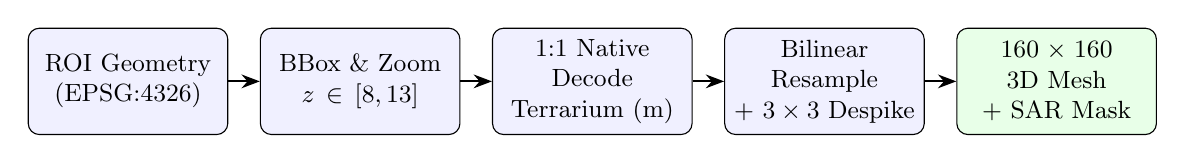
\begin{tikzpicture}[node distance=4mm,
  caja/.style={draw,rounded corners,fill=blue!6,align=center,text width=2.3cm,minimum height=1.35cm,font=\small},
  sal/.style={caja,fill=green!9},
  fl/.style={-{Stealth},thick}]
\node[caja] (a) {ROI Geometry\\(EPSG:4326)};
\node[caja,right=of a] (b) {BBox \& Zoom\\$z\in[8,13]$};
\node[caja,right=of b] (c) {1:1 Native Decode\\Terrarium (m)};
\node[caja,right=of c] (d) {Bilinear Resample\\+ $3\times3$ Despike};
\node[sal,right=of d] (e) {$160\times160$ 3D Mesh\\+ SAR Mask};
\draw[fl] (a)--(b); \draw[fl] (b)--(c); \draw[fl] (c)--(d); \draw[fl] (d)--(e);
\end{tikzpicture}
\caption{Client-side processing pipeline of the 3D Terrain Viewer (\src{web/src/utils/terrain3d.ts}).
RGB-to-meters elevation decoding occurs at native $1:1$ tile resolution prior to any spatial interpolation.}
\label{fig:flujo-relieve3d}
\end{figure}

\section{Mathematical Formulation of the Elevation Mesh}
\label{sec:relieve3d-matematicas}

\subsection{Bounding Box, Web Mercator Projection, and Zoom Selection}
\label{sec:relieve3d-mercator}

Given an active ROI geometry in WGS84 geographic coordinates ($\mathrm{EPSG}{:}4326$)---whether a \texttt{Polygon}, an administrative \texttt{MultiPolygon}, or a manually drawn coordinate ring---the function \texttt{bboxFromGeometry} extracts its geographic bounding box:
\begin{equation}
  \mathcal{B} = [\lambda_{\min},\ \varphi_{\min},\ \lambda_{\max},\ \varphi_{\max}],
  \label{eq:bbox-relieve}
\end{equation}
where $\lambda\in[-180^\circ,180^\circ]$ is longitude and $\varphi\in[-85.0511^\circ,85.0511^\circ]$ is latitude clamped to the Web Mercator ($\mathrm{EPSG}{:}3857$) domain. To prevent excessive client tile downloads, the angular span is bounded to $\Delta\lambda = \lambda_{\max}-\lambda_{\min}\le 3^\circ$ and $\Delta\varphi = \varphi_{\max}-\varphi_{\min}\le 3^\circ$.

At integer zoom level $z\in[8,13]$, the Web Mercator pyramid has $2^z$ tiles per axis. Continuous tile coordinates $(X_t,Y_t)\in[0,2^z)$ are given by the spherical Mercator transformation:
\begin{equation}
  X_t(\lambda,z) = \frac{\lambda + 180^\circ}{360^\circ}\,2^z,
  \qquad
  Y_t(\varphi,z) = \frac{1}{2}\left[
    1 - \frac{1}{\pi}\ln\!\left(\tan\!\left(\frac{\varphi\pi}{180^\circ}\right)
    + \sec\!\left(\frac{\varphi\pi}{180^\circ}\right)\right)
  \right] 2^z .
  \label{eq:mercator-tiles}
\end{equation}
The integer tile indices covering $\mathcal{B}$ are $x_0=\lfloor X_t(\lambda_{\min},z)\rfloor$, $x_1=\lfloor X_t(\lambda_{\max},z)-10^{-9}\rfloor$, $y_0=\lfloor Y_t(\varphi_{\max},z)\rfloor$, and $y_1=\lfloor Y_t(\varphi_{\min},z)-10^{-9}\rfloor$ (where $Y_t$ increases from North to South). The function \texttt{chooseZoom} selects the highest resolution level whose total tile count does not exceed the budget $N_{\max}=36$ tiles:
\begin{equation}
  z^\ast = \max\Bigl\{\, z\in\{8,9,10,11,12,13\} \;\Big|\;
  (x_1 - x_0 + 1)(y_1 - y_0 + 1) \le N_{\max} \,\Bigr\}.
  \label{eq:choose-zoom}
\end{equation}

The horizontal metric dimensions $(W_m,H_m)$ of bounding box $\mathcal{B}$---required both to preserve the true horizontal aspect ratio of the 3D block and to compute terrain slope derivatives in meters per meter---are evaluated on the mean Earth sphere of radius $R_\oplus = 6,371,008.8\,\unit{m}$ at mid-latitude $\bar\varphi = (\varphi_{\min}+\varphi_{\max})/2$:
\begin{equation}
  W_m = R_\oplus\,\frac{(\lambda_{\max}-\lambda_{\min})\pi}{180^\circ}\,\cos\!\left(\frac{\bar\varphi\pi}{180^\circ}\right),
  \qquad
  H_m = R_\oplus\,\frac{(\varphi_{\max}-\varphi_{\min})\pi}{180^\circ}.
  \label{eq:bbox-metros}
\end{equation}

\subsection{Native 1:1 Decoding of AWS Terrarium Tiles}
\label{sec:relieve3d-terrarium}

Terrain elevation is sourced from open \textbf{AWS Terrarium} tiles ($256\times256$ 8-bit RGB PNGs derived from SRTM/NASADEM and public elevation datasets). Each pixel encodes elevation in meters across its red $R$, green $G$, and blue $B$ byte channels ($R,G,B\in\{0,1,\ldots,255\}$):
\begin{equation}
  h_{\mathrm{raw}}(R,G,B) = \left(256\,R + G + \frac{B}{256}\right) - 32,768\quad[\unit{m}].
  \label{eq:terrarium-decode}
\end{equation}
In this base-256 fixed-point encoding:
\begin{itemize}
  \item Channel $R$ contributes coarse $256\,\unit{m}$ steps (with $R=128, G=0, B=0$ representing exactly $0\,\unit{m}$ sea level).
  \item Channel $G$ contributes integer meters ($0$ to $255\,\unit{m}$).
  \item Channel $B$ contributes sub-meter fractions with resolution $1/256\,\unit{m}\approx 3.9\,\unit{mm}$.
\end{itemize}

\warn{Terrarium PNG images must never be scaled or interpolated in RGB color space prior to applying Equation~\eqref{eq:terrarium-decode}. If a pixel at $h=255\,\unit{m}$ ($R=128,G=255,B=0$) and an adjacent pixel at $h=256\,\unit{m}$ ($R=129,G=0,B=0$) are linearly blended in RGB space, the intermediate pixel receives $R=128,G=128$ ($h=128\,\unit{m}$) or, if $R$ rounds up to $129$ while $G$ remains high, creates a spurious $+256\,\unit{m}$ single-vertex needle spike. To prevent this, \src{web/src/utils/terrain3d.ts} decodes each tile via \texttt{createImageBitmap(blob, \{colorSpaceConversion: 'none'\})} onto a native $1:1$ ($256\times256$) canvas with \texttt{imageSmoothingEnabled = false} and immediately converts every pixel into a metric \texttt{Float32Array}.}

\subsection{Coastal Sanitization and Bathymetry Clamping}
\label{sec:relieve3d-saneamiento}

Along coastal regions (such as the Acapulco ROI), Terrarium tiles contain deep ocean bathymetry descending to $-9,651\,\unit{m}$. Allowing negative submarine depths into the 3D terrain block would artificially inflate total relief $\Delta z$ beyond $10,000\,\unit{m}$, distorting the side walls and compressing terrestrial hypsometric colors into a flat uniform hue.

The function \texttt{sanitizeElevationSample} verifies full alpha opacity ($\alpha=255$), rejects corrupted values above the physical ceiling $h_{\mathrm{ceil}}=9,000\,\unit{m}$, and clamps negative elevations to sea level $h_{\mathrm{floor}}=0\,\unit{m}$:
\begin{equation}
  h_{\mathrm{san}}(R,G,B,\alpha) =
  \begin{cases}
    \mathrm{NaN}, & \text{if } \alpha < 255 \;\vee\; \neg\text{finite}(h_{\mathrm{raw}}) \;\vee\; h_{\mathrm{raw}} > 9,000\,\unit{m},\\[4pt]
    \max\bigl(0\,\unit{m},\ h_{\mathrm{raw}}(R,G,B)\bigr), & \text{otherwise.}
  \end{cases}
  \label{eq:saneamiento-costero}
\end{equation}
Thus, ocean surfaces render flat at $0\,\unit{m}$ and reported minimum/maximum elevations reflect exclusively emergent land within the ROI.

\subsection{Bilinear Resampling in Meters onto the \texorpdfstring{$161\times161$}{161x161} Mesh}
\label{sec:relieve3d-bilineal}

Once the native sanitized elevation mosaic $M(x,y)$ in meters ($W_s\times H_s$ pixels) is assembled, the continuous sub-window $[s_x, s_x+s_w]\times[s_y, s_y+s_h]$ matching bounding box $\mathcal{B}$ is resampled onto the 3D mesh grid of $N_c\times N_r = 161\times161$ vertices ($160\times160$ segments).

For each vertex $(c,r)$ with $c\in\{0,\ldots,N_c-1\}$ and $r\in\{0,\ldots,N_r-1\}$, the continuous source mosaic coordinates are:
\begin{equation}
  f_x = s_x + \frac{c}{N_c - 1}\,s_w,
  \qquad
  f_y = s_y + \frac{r}{N_r - 1}\,s_h,
\end{equation}
with base indices $x_0=\lfloor f_x\rfloor$, $y_0=\lfloor f_y\rfloor$, $x_1=\min(W_s-1,x_0+1)$, $y_1=\min(H_s-1,y_0+1)$ and fractional weights $t_x = f_x - x_0$, $t_y = f_y - y_0$. When all four neighboring samples $h_{00}=M(x_0,y_0)$, $h_{10}=M(x_1,y_0)$, $h_{01}=M(x_0,y_1)$, and $h_{11}=M(x_1,y_1)$ are finite, \texttt{resampleElevationBilinear} evaluates bilinear interpolation directly in meters:
\begin{equation}
  h(c,r) = (1 - t_y)\bigl[(1 - t_x)h_{00} + t_x h_{10}\bigr]
         + t_y\bigl[(1 - t_x)h_{01} + t_x h_{11}\bigr].
  \label{eq:bilineal-metros}
\end{equation}
If any neighbor is $\mathrm{NaN}$, the function falls back to the average of available finite neighbors in the $2\times2$ cell.

\subsection{Conditional \texorpdfstring{$3\times3$}{3x3} Anti-Spike Filter (\texttt{despikeElevationGrid})}
\label{sec:relieve3d-despike}

Even under native $1:1$ decoding, an upstream tile may occasionally contain an isolated corrupted pixel. To suppress single-vertex needle spikes without blunting genuine canyon rims or mountain ridges, \texttt{despikeElevationGrid} applies a conditional median filter over the punctured 8-neighbor ring $\mathcal{N}_{3\times3}(c,r)$:
\begin{equation}
  \mathcal{N}_{3\times3}(c,r) = \Bigl\{\, h(c+\delta_c,\ r+\delta_r) \;\Big|\;
  \delta_c,\delta_r\in\{-1,0,1\},\ (\delta_c,\delta_r)\neq(0,0) \,\Bigr\}.
\end{equation}
Let $m_{c,r} = \operatorname{median}\bigl(\mathcal{N}_{3\times3}(c,r)\bigr)$ denote the median of the finite neighbors. Using a single-step spike threshold $\tau_{\mathrm{spike}} = 80\,\unit{m}$, the filtered elevation $\tilde{h}(c,r)$ is:
\begin{equation}
  \tilde{h}(c,r) =
  \begin{cases}
    m_{c,r}, & \text{if } \bigl|h(c,r) - m_{c,r}\bigr| > \tau_{\mathrm{spike}} \;\vee\; \neg\text{finite}\bigl(h(c,r)\bigr),\\[4pt]
    h(c,r), & \text{otherwise.}
  \end{cases}
  \label{eq:despike}
\end{equation}
On a real continuous slope (e.g., inside Sumidero Canyon), the 8 neighbors bracket the central value symmetrically, so $|h(c,r)-m_{c,r}|\approx 0$ and the true slope remains untouched. Conversely, an isolated $+256\,\unit{m}$ byte-jump spike exceeds $\tau_{\mathrm{spike}}=80\,\unit{m}$ and is cleanly replaced by $m_{c,r}$.

Final ROI relief telemetry metrics are evaluated after despiking:
\begin{equation}
  h_{\min} = \min_{c,r} \tilde{h}(c,r),
  \qquad
  h_{\max} = \max_{c,r} \tilde{h}(c,r),
  \qquad
  \Delta z = h_{\max} - h_{\min}.
  \label{eq:telemetria-relieve}
\end{equation}

\begin{ejemplo}[Effect of the Anti-Spike Filter on a Slope with a $+256\,\unit{m}$ Needle]
Consider a $3\times3$ subgrid on a uniform planar slope rising $20\,\unit{m}$ per column Eastward and $15\,\unit{m}$ per row Southward, centered at $570\,\unit{m}$. The 8 neighbors have elevations $\{535, 555, 575, 550, 590, 565, 585, 605\}\,\unit{m}$, whose sorted median is $m = 0.5\times(565+575) = 570\,\unit{m}$. If the central vertex suffers a $+256\,\unit{m}$ red-channel byte jump to $570 + 256 = 826\,\unit{m}$, its deviation from the neighborhood median is $|826 - 570| = 256\,\unit{m} > 80\,\unit{m}$. Equation~\eqref{eq:despike} restores the center vertex to $570\,\unit{m}$ without altering a single millimeter of the surrounding slope (verified in \src{web/tests/terrain3d.test.mjs}).
\end{ejemplo}

\subsection{3D Block Geometry, Vertical Exaggeration, and Slate Pedestal}
\label{sec:relieve3d-bloque}

In the Three.js scene (\src{web/src/components/Terrain3DViewer.tsx}), the longer horizontal side of the ROI is normalized to $L_0 = 100$ scene units via the metric scale factor:
\begin{equation}
  k = \frac{L_0}{\max(W_m,\ H_m,\ 1\,\unit{m})},
  \qquad
  W = k\,W_m,
  \qquad
  H = k\,H_m.
  \label{eq:escala-escena}
\end{equation}
Given the user-controlled vertical exaggeration factor $E_v \in [1.0, 5.0]$ (defaulting to $E_v = 2.0$), the vertical displacement of each \texttt{PlaneGeometry} vertex above the ROI base elevation is:
\begin{equation}
  Z(c,r) = k\,E_v\,\bigl(\tilde{h}(c,r) - h_{\min}\bigr) \ge 0.
  \label{eq:z-vertice}
\end{equation}
To give the model a clean architectural cross-section appearance rather than a bulky cube, the four side walls and bottom plate (rendered in dark slate \texttt{\#334155} and \texttt{\#1e293b}) extend to a fixed pedestal depth equal to $3.5\,\text{\%}$ of the longer horizontal dimension, independent of $E_v$:
\begin{equation}
  Z_{\mathrm{base}} = -0.035\,\max(W, H).
  \label{eq:zocalo-fijo}
\end{equation}

\begin{figure}[htbp]
  \centering
  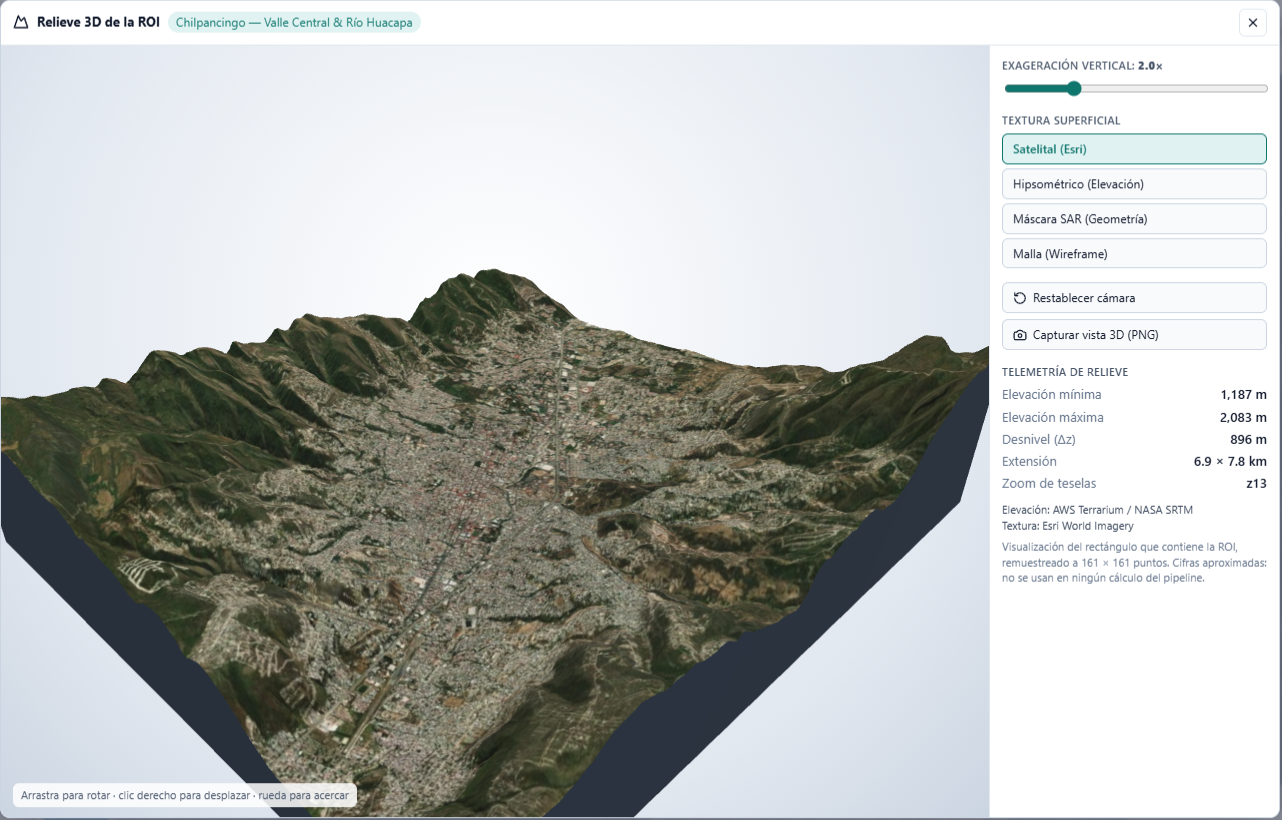
\includegraphics[width=0.82\textwidth]{fig/IMG_visor_3d_satelital.png}
  \caption{Interactive 3D topographic block model in \texttt{Terrain3DViewer} with \emph{Satellite (Esri World Imagery)} texture, $2.0\times$ vertical exaggeration, thin dark-slate pedestal, and right-hand controls and telemetry sidebar ($\Delta z$, $h_{\min}$, $h_{\max}$, extent, and tile zoom).}
  \label{fig:visor-3d-satelital}
\end{figure}

\subsection{Lambertian Directional Hillshading (Hypsometric Mode)}
\label{sec:relieve3d-hillshade}

When the user selects \textbf{Hypsometric (Elevation)} texture mode, \texttt{hypsometricCanvas} blends an altitudinal color ramp with analytical Lambertian hillshading. Let $t = (\tilde{h} - h_{\min})/\max(h_{\max}-h_{\min},1)\in[0,1]$ denote normalized elevation:
\begin{itemize}
  \item If the ROI reaches sea level ($h_{\min}\le 0.5\,\unit{m}$) and a vertex satisfies $\tilde{h}(c,r)\le 0.5\,\unit{m}$, it is assigned a constant coastal blue $\mathrm{RGB}=(38,118,178)$ without slope shading.
  \item For emergent terrain, color is piecewise linearly interpolated across lowland green $(38,115,77)$ at $t=0$, light green $(110,168,88)$ at $t=0.20$, mid-slope ochre $(224,206,128)$ at $t=0.45$, montane brown $(166,112,68)$ at $t=0.72$, alpine rock gray $(132,108,94)$ at $t=0.90$, and summit white $(245,245,245)$ at $t=1.0$.
\end{itemize}
With horizontal grid spacings $\Delta x = W_m/(N_c-1)$ and $\Delta y = H_m/(N_r-1)$, centered finite-difference gradients scaled by visual enhancement factor $f_z = 2.2$ are:
\begin{equation}
  p = f_z\,\frac{\tilde{h}(c+1,r) - \tilde{h}(c-1,r)}{2\,\Delta x},
  \qquad
  q = f_z\,\frac{\tilde{h}(c,r-1) - \tilde{h}(c,r+1)}{2\,\Delta y},
  \label{eq:grad-hillshade}
\end{equation}
where $x$ increases Eastward and $y$ increases Northward (while row index $r$ increases Southward). Illuminating from the Northwest (azimuth $315^\circ$, elevation $42^\circ$) with unit light vector $\hat{\mathbf{s}} = (-0.526,\ 0.526,\ 0.669)$, the dot product with unit surface normal $\hat{\mathbf{n}} = (-p,-q,1)/\sqrt{p^2+q^2+1}$ modulates each RGB channel $C\in\{R,G,B\}$ via:
\begin{equation}
  \cos\gamma = \frac{-p\,s_x - q\,s_y + s_z}{\sqrt{p^2 + q^2 + 1}},
  \qquad
  S = \operatorname{clip}\!\bigl(0.45 + 0.85\max(0,\cos\gamma),\ 0.48,\ 1.22\bigr),
  \qquad
  C_{\mathrm{out}} = \min\bigl(255,\ \operatorname{round}(C\cdot S)\bigr).
  \label{eq:lambert-hillshade}
\end{equation}

\begin{figure}[htbp]
  \centering
  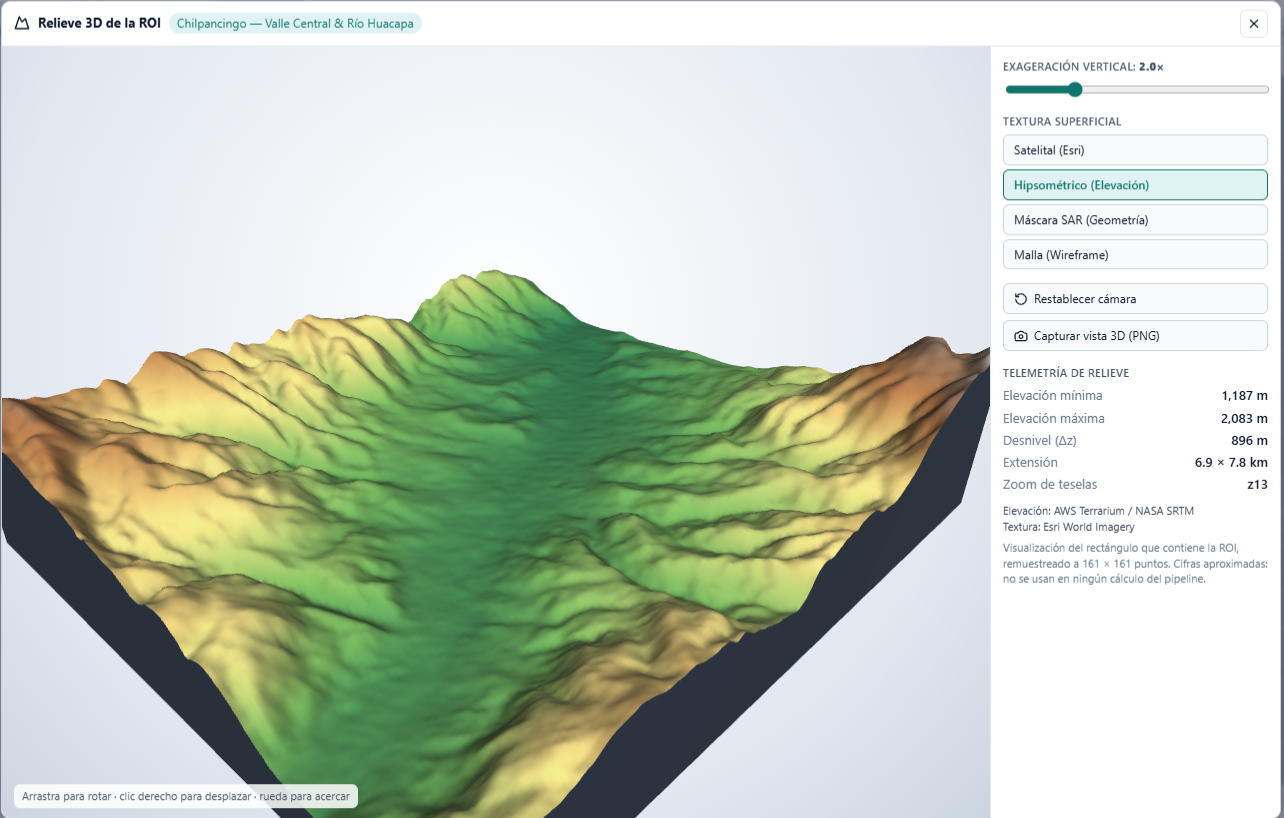
\includegraphics[width=0.82\textwidth]{fig/IMG_visor_3d_hipsometrico.png}
  \caption{The same ROI rendered in \emph{Hypsometric (Elevation)} mode inside the 3D viewer. Coastal blue delineates $0\,\unit{m}$ water bodies, while the elevation color ramp and Lambertian hillshading~\eqref{eq:lambert-hillshade} highlight watershed divides and canyon walls.}
  \label{fig:visor-3d-hipsometrico}
\end{figure}

\section{3D SAR Geometric Feasibility Mask: Critical Slope, Layover, and Shadow}
\label{sec:relieve3d-mascara-sar}

As explained in Section~\ref{sec:gcov}, NISAR GCOV products apply Radiometric Terrain Correction (RTC) to normalize illuminated area, but current catalog releases set \texttt{shadowMaskingApplied = False}: pixels compromised by topographic inversion (\emph{layover}) or beam occlusion (radar shadow) are not flagged in the product \texttt{mask} layer. The 3D viewer's \textbf{SAR Mask (Geometry)} texture mode computes and drapes directly onto the 3D terrain mesh a diagnostic map showing where radar backscatter measurements are geometrically reliable and where severe relief distortions dominate.

\begin{intuicion}
Imagine illuminating a 3D mountain scale model with a flashlight held to one side at $43^\circ$ from the vertical (NISAR's nominal incidence angle $\theta_i$):
\begin{itemize}
  \item Over \textbf{gentle valleys and plains} ($\alpha \le 15^\circ$), the beam illuminates the ground smoothly: temporal backscatter changes ($\Delta\gamma^0$) reliably reflect surface changes.
  \item On \textbf{steep cliffs facing directly toward the flashlight} at slopes $\ge 43^\circ$, the mountain crest lies closer to the flashlight than the cliff base. Echoes from the summit and base arrive simultaneously mixed together: this is \textbf{\emph{layover}} (mapped in red).
  \item On \textbf{steep back-slopes facing away from the flashlight} at angles steeper than the grazing ray ($90^\circ - 43^\circ = 47^\circ$), the beam skims right over the ridge crest leaving the lee slope in darkness: this is \textbf{radar shadow} (mapped in deep indigo).
\end{itemize}
When the satellite switches from an Ascending orbit (illuminating from East to West) to a Descending orbit (illuminating from West to East), cliffs that were in \emph{layover} flip into radar shadow and vice versa.
\end{intuicion}

\subsection{NISAR Left-Looking Side-Incidence Geometry}
\label{sec:relieve3d-geometria-nisar}

Unlike right-looking SAR missions, NISAR's L-band radar is \textbf{left-looking} (\texttt{lookDirection = Left}):
\begin{itemize}
  \item \textbf{Ascending Orbit (e.g., stack T62/F10):} the spacecraft flies South-to-North along a heading of $\approx 350^\circ$ (tilted slightly West by orbital inclination). Looking $90^\circ$ to its left, the radar pulse propagates from the satellite toward the ground along horizontal azimuth $\psi_{\mathrm{asc}} \approx 260^\circ$ (West-Southwest).
  \item \textbf{Descending Orbit (e.g., stack T55/F80):} the spacecraft flies North-to-South along a heading of $\approx 190^\circ$. Looking $90^\circ$ to its left, the radar pulse propagates from the satellite toward the ground along horizontal azimuth $\psi_{\mathrm{desc}} \approx 100^\circ$ (East-Southeast).
\end{itemize}

Letting $\psi \in \{260^\circ, 100^\circ\}$ denote the horizontal beam propagation azimuth measured clockwise from North, the horizontal unit look vector in local East--North coordinates is:
\begin{equation}
  \hat{\mathbf{l}}_{\mathrm{h}} = (l_x,\ l_y) = \left(\sin\psi,\ \cos\psi\right).
  \label{eq:vector-haz-sar}
\end{equation}

\subsection{True Metric Terrain Derivatives and Radar-Projected Slope}
\label{sec:relieve3d-ecuaciones-sar}

At every vertex $(c,r)$ of the despiked elevation grid $\tilde{h}$, \texttt{computeSarGeometricMask} evaluates the true physical partial derivatives (unexaggerated, in dimensionless $\unit{m/m}$) via centered finite differences in the interior and one-sided differences along the boundary edges:
\begin{equation}
  z_x(c,r) = \frac{\partial \tilde{h}}{\partial x}
  \approx \frac{\tilde{h}(c_{\mathrm{next}},r) - \tilde{h}(c_{\mathrm{prev}},r)}{(c_{\mathrm{next}} - c_{\mathrm{prev}})\,\Delta x},
  \qquad
  z_y(c,r) = \frac{\partial \tilde{h}}{\partial y}
  \approx \frac{\tilde{h}(c,r_{\mathrm{prev}}) - \tilde{h}(c,r_{\mathrm{next}})}{(r_{\mathrm{next}} - r_{\mathrm{prev}})\,\Delta y}.
  \label{eq:derivadas-reales-sar}
\end{equation}
From $(z_x, z_y)$, two fundamental geometric quantities are derived:
\begin{enumerate}
  \item \textbf{True topographic slope magnitude $\alpha$:}
        \begin{equation}
          \tan\alpha(c,r) = \sqrt{z_x^2(c,r) + z_y^2(c,r)},
          \qquad
          \alpha(c,r) = \arctan\sqrt{z_x^2(c,r) + z_y^2(c,r)}.
          \label{eq:pendiente-real}
        \end{equation}
  \item \textbf{Directional slope projected along the radar beam propagation vector ($s_{\mathrm{rad}}$):}
        \begin{equation}
          s_{\mathrm{rad}}(c,r) = \nabla\tilde{h}(c,r)\cdot\hat{\mathbf{l}}_{\mathrm{h}}
          = z_x(c,r)\,l_x + z_y(c,r)\,l_y,
          \qquad
          \alpha_{\mathrm{rad}}(c,r) = \arctan\bigl(s_{\mathrm{rad}}(c,r)\bigr).
          \label{eq:pendiente-proyectada}
        \end{equation}
\end{enumerate}

The sign of $s_{\mathrm{rad}}$ carries direct physical meaning:
\begin{itemize}
  \item When $s_{\mathrm{rad}} > 0$, terrain elevation \emph{rises} along the advancing radar wave direction $\hat{\mathbf{l}}_{\mathrm{h}}$---meaning the slope \textbf{faces toward the incoming radar beam}.
  \item When $s_{\mathrm{rad}} < 0$, terrain elevation \emph{drops} along the advancing wave direction---meaning the slope \textbf{faces away from the incoming radar beam}.
\end{itemize}

\subsection{Four-Class Classification Thresholds}
\label{sec:relieve3d-clases-sar}

Using nominal incidence angle $\theta_i = 43^\circ$ (representative of the Chiapas ROI swath where $\theta_i\in[42.3^\circ,45.4^\circ]$, Figure~E in Section~\ref{sec:figuras}) and critical slope threshold $\alpha_c = 15^\circ$, each vertex $(c,r)$ is classified in strict priority order:
\begin{equation}
  \mathrm{Class}(c,r) =
  \begin{cases}
    \text{\textbf{Layover / severe foreshortening}}, &
      \text{if } s_{\mathrm{rad}}(c,r) \ge \tan\theta_i
      \quad\bigl(\alpha_{\mathrm{rad}} \ge \theta_i\bigr),\\[6pt]
    \text{\textbf{Radar shadow}}, &
      \text{if } -s_{\mathrm{rad}}(c,r) \ge \tan(90^\circ - \theta_i)
      \quad\bigl(-\alpha_{\mathrm{rad}} \ge 90^\circ - \theta_i\bigr),\\[6pt]
    \text{\textbf{Critical slope}}, &
      \text{if } \sqrt{z_x^2 + z_y^2} > \tan\alpha_c
      \quad\bigl(\alpha > 15^\circ\text{ without layover or shadow}\bigr),\\[6pt]
    \text{\textbf{Reliable}}, &
      \text{otherwise} \quad\bigl(\alpha \le 15^\circ\text{ without layover or shadow}\bigr).
  \end{cases}
  \label{eq:clasificacion-sar}
\end{equation}

For $\theta_i = 43^\circ$ and $\alpha_c = 15^\circ$, the three dimensionless slope thresholds evaluate to:
\begin{equation}
  \tan 15^\circ \approx 0.2679,
  \qquad
  \tan 43^\circ \approx 0.9325,
  \qquad
  \tan(90^\circ - 43^\circ) = \tan 47^\circ \approx 1.0724.
\end{equation}

\begin{table}[htbp]
\centering\small
\begin{tabularx}{\linewidth}{p{.23\linewidth}p{.16\linewidth}p{.24\linewidth}X}
\toprule
\textbf{Category} & \textbf{Color} & \textbf{Geometric Condition} & \textbf{Implication for Interpreting $\Delta\gamma^0$}\\\midrule
Reliable & Green \texttt{\#22C55E} & $\alpha \le 15^\circ$, no layover/shadow & Stable viewing geometry; optimal terrain for quantifying soil moisture, flood, or vegetation change.\\
Critical slope & Amber \texttt{\#F59E0B} & $\alpha > 15^\circ$, no layover/shadow & Moderate foreshortening; RTC area normalization operates near DEM resolution limits.\\
Layover / foreshortening & Red \texttt{\#EF4444} & $s_{\mathrm{rad}} \ge \tan\theta_i$ & Topographic folding mixing crest and base echoes; do not interpret pixel-level $\Delta\gamma^0$.\\
Radar shadow & Indigo \texttt{\#1E1B4B} & $-s_{\mathrm{rad}} \ge \tan(90^\circ-\theta_i)$ & Occluded lee slope receiving no direct beam energy; dominated by receiver thermal noise.\\\bottomrule
\end{tabularx}
\caption{SAR geometric feasibility mask categories in the 3D Terrain Viewer (\texttt{computeSarGeometricMask}).}
\label{tab:clases-mascara-sar}
\end{table}

Across all $N_{\mathrm{tot}} = N_c N_r = 25,921$ mesh vertices, the percentage of ROI area in each geometric regime is reported in the live telemetry sidebar:
\begin{equation}
  P_k = 100\,\frac{N_k}{N_{\mathrm{tot}}}\,\mathrm{\%},
  \qquad
  k \in \{\text{reliable},\ \text{critical},\ \text{layover},\ \text{shadow}\},
  \qquad
  \sum_k P_k = 100\,\mathrm{\%}.
  \label{eq:porcentajes-sar}
\end{equation}

\begin{ejemplo}[Layover-to-Shadow Inversion When Switching Orbits on a Canyon Wall]
Consider a steep canyon wall in Sumidero Canyon rising Westward at a constant gradient of $+200\,\unit{m}$ per $100\,\unit{m}$ horizontal distance ($z_x = -2.0$, $z_y = 0$, i.e., $\alpha = \arctan(2.0) = 63.4^\circ$):
\begin{itemize}
  \item \textbf{In Ascending Orbit ($\psi = 260^\circ$):} $l_x = \sin 260^\circ = -0.9848$. The radar-projected slope is $s_{\mathrm{rad}} = (-2.0)(-0.9848) = +1.9696$. Since $1.9696 \ge \tan 43^\circ = 0.9325$, the entire cliff is classified as \textbf{Layover} ($100\,\mathrm{\%}$).
  \item \textbf{In Descending Orbit ($\psi = 100^\circ$):} $l_x = \sin 100^\circ = +0.9848$. Now the radar-projected slope reverses sign to $s_{\mathrm{rad}} = (-2.0)(+0.9848) = -1.9696$. Since $-s_{\mathrm{rad}} = 1.9696 \ge \tan 47^\circ = 1.0724$, the exact same canyon wall flips completely into \textbf{Radar Shadow} ($100\,\mathrm{\%}$).
\end{itemize}
This explains why the 3D viewer provides a live toggle between \emph{Ascending (T62/F10)} and \emph{Descending (T55/F80)}, and visually demonstrates why opposite orbital passes must never be mixed in a $\Delta\gamma^0$ difference map.
\end{ejemplo}

\begin{figure}[htbp]
  \centering
  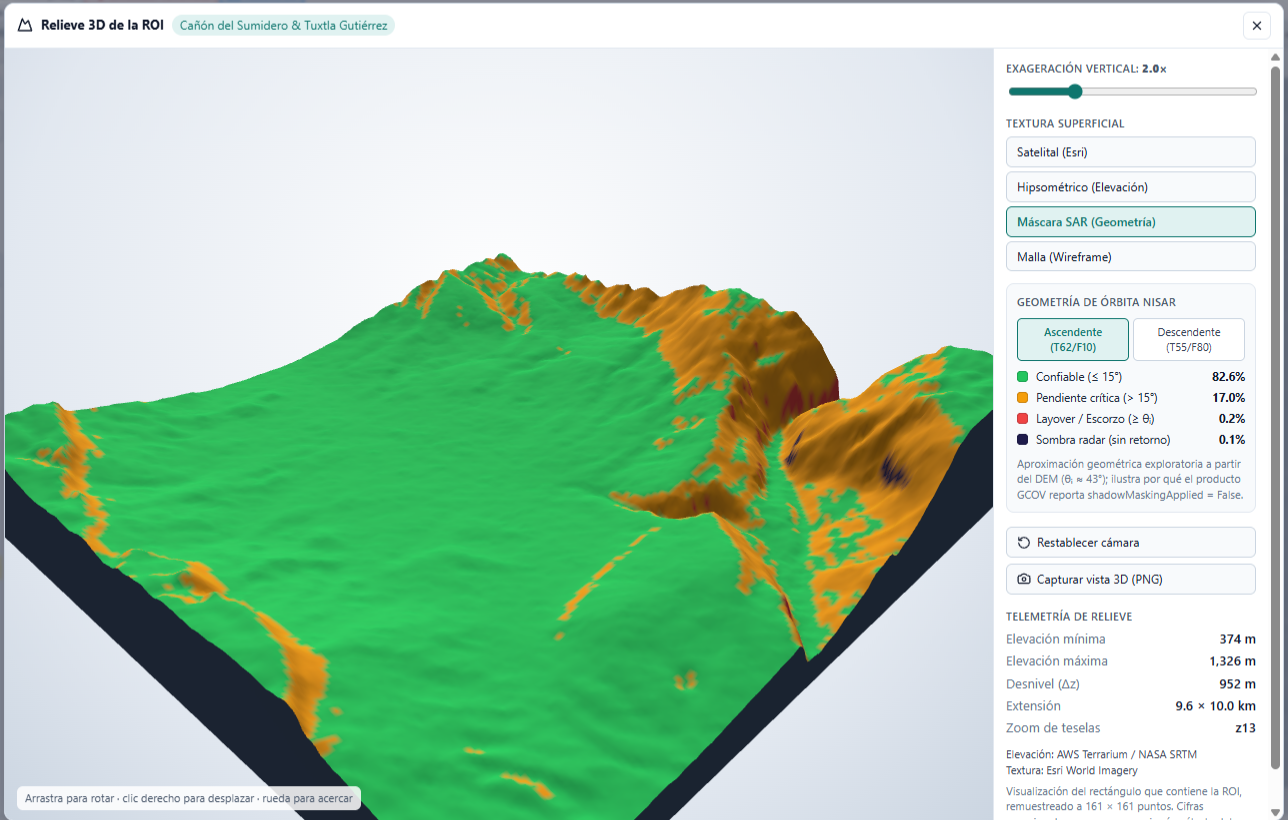
\includegraphics[width=0.82\textwidth]{fig/IMG_visor_3d_mascara_sar_asc.png}
  \caption{\emph{SAR Mask (Geometry)} mode draped over the 3D terrain block for the \textbf{Ascending (T62/F10)} pass.
  Green delineates reliable valleys and plains ($\alpha\le 15^\circ$), amber marks critical slopes ($>15^\circ$), and red/indigo highlight canyon walls affected by \emph{layover} and radar shadow.}
  \label{fig:visor-3d-sar-asc}
\end{figure}

\begin{figure}[htbp]
  \centering
  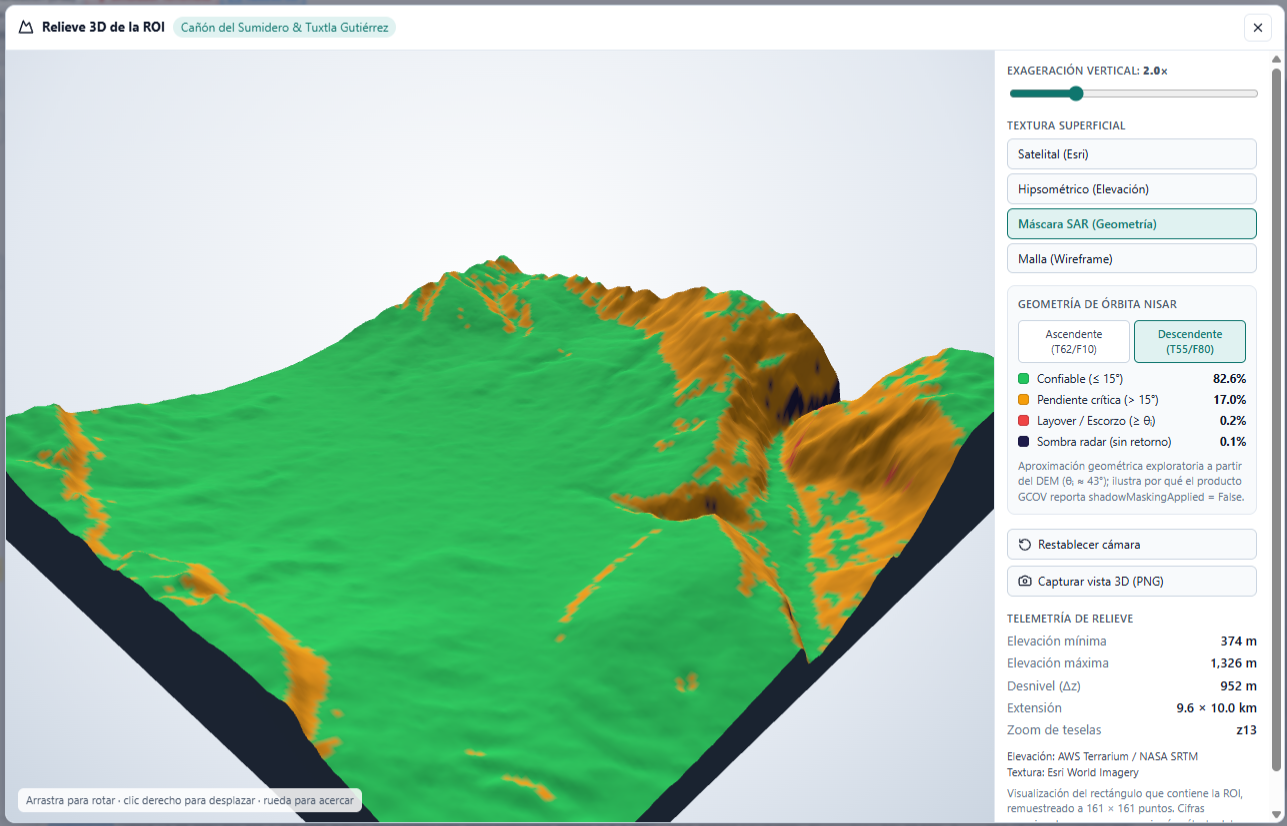
\includegraphics[width=0.82\textwidth]{fig/IMG_visor_3d_mascara_sar_desc.png}
  \caption{Geometric inversion upon toggling to the \textbf{Descending (T55/F80)} pass in the 3D viewer sidebar. East/West-facing canyon walls swap their \emph{layover} (red) and radar shadow (deep indigo) regimes, updating class percentages in real time.}
  \label{fig:visor-3d-sar-desc}
\end{figure}

\section{WebGL Memory Management and Module Verification}
\label{sec:relieve3d-webgl}

To ensure that repeatedly opening and closing the 3D modal never leaks GPU memory or exhausts browser WebGL contexts needed by MapLibre GL, \texttt{Terrain3DViewer} executes a deterministic teardown sequence on unmount:
\begin{enumerate}
  \item Cancels the animation frame loop (\texttt{cancelAnimationFrame}) and disconnects the \texttt{ResizeObserver}.
  \item Disposes the \texttt{OrbitControls} instance (\texttt{controls.dispose()}).
  \item Explicitly disposes all GPU buffers across the three geometries (\texttt{surfaceGeom}, \texttt{wallGeom}, \texttt{bottomGeom}), four materials (\texttt{surfaceMat}, \texttt{wireMat}, \texttt{wallMat}, \texttt{bottomMat}), and all allocated \texttt{CanvasTexture} instances.
  \item Invokes \texttt{renderer.dispose()}, forces native WebGL context release via \texttt{renderer.forceContextLoss()}, and removes the \texttt{<canvas>} element from the DOM.
\end{enumerate}

The automated test suite \src{web/tests/terrain3d.test.mjs} independently verifies native Terrarium decoding~\eqref{eq:terrarium-decode}, bounding-box extraction, Web Mercator tile selection~\eqref{eq:mercator-tiles}, coastal sanitization~\eqref{eq:saneamiento-costero}, $+256\,\unit{m}$ spike removal~\eqref{eq:despike} without slope distortion, SAR geometric classification~\eqref{eq:clasificacion-sar} across flat plains and cliffs for both orbital passes, ES/EN i18n completeness, and WebGL teardown calls.

\part{Derivations and Mathematical Proofs}
\label{part:derivaciones}

This part compiles the step-by-step mathematical derivations supporting equations stated earlier without proof, allowing readers to verify each result directly within this document. Each derivation states its physical assumptions, derives the closed-form result, and references the section where it is applied.

\section{Speckle Statistics}
\label{sec:der-speckle}

\subsection{Fully Developed Single-Look Speckle Intensity Is Exponentially Distributed}

Starting from the coherent phasor sum in Equation~\eqref{eq:fasor}, $z=x+\mathrm{i}y$, with a large number of elementary scatterers $M$ and independent uniformly distributed phases $\varphi_k \sim \mathcal{U}[0,2\pi)$, the Central Limit Theorem implies that the real and imaginary parts $x$ and $y$ are independent zero-mean Gaussian random variables with identical variance $s^2$. Their joint probability density is:
\[
  p(x,y)=\frac{1}{2\pi s^2}\,e^{-(x^2+y^2)/(2s^2)} .
\]
Transforming to polar coordinates $(\rho,\phi)$ via $x=\rho\cos\phi$, $y=\rho\sin\phi$ with area element $\rho\,\dd\rho\,\dd\phi$, and integrating over $\phi\in[0,2\pi)$ yields the Rayleigh amplitude density $p(\rho)=(\rho/s^2)\,e^{-\rho^2/(2s^2)}$. Changing variables to linear intensity (power) $P=\rho^2$ with $\dd P=2\rho\,\dd\rho$ gives:
\begin{equation}
  p(P)=\frac{1}{2s^2}\,e^{-P/(2s^2)}=\frac{1}{\bar{P}}\,e^{-P/\bar{P}},
  \qquad \bar{P}=2s^2 .
  \label{eq:der-exp}
\end{equation}
This is an exponential distribution with mean $\mathbb{E}[P]=\bar{P}$ and variance $\mathrm{Var}[P]=\bar{P}^2$, proving that the standard deviation equals the mean (unit coefficient of variation, Section~\ref{sec:speckle}).

\subsection{The $L$-Look Linear Average Follows a Gamma Distribution}

The sum of $L$ independent exponential random variables of mean $\bar{P}$ follows a Gamma distribution of shape $L$ and scale $\bar{P}$. Dividing by $L$ scales the distribution to $\mathrm{Gamma}(L, \bar{P}/L)$, whose mean and variance are:
\[
  \mathbb{E}[\bar P_L]=\bar{P},\qquad
  \mathrm{Var}[\bar P_L]=\frac{\bar{P}^2}{L},
\]
yielding the $1/\sqrt L$ coefficient of variation in Equation~\eqref{eq:gamma-ml}.

\subsection{Expected Value and Variance of Log-Transformed Speckle}

For a Gamma-distributed variable $X \sim \mathrm{Gamma}(L,\theta)$, standard integral identities give $\mathbb{E}[\ln X]=\psi(L)+\ln\theta$ and $\mathrm{Var}[\ln X]=\psi'(L)$, where $\psi(z)=\Gamma'(z)/\Gamma(z)$ is the digamma function and $\psi'(z)$ is the trigamma function. Substituting $\theta=\bar{P}/L$ and $10\log_{10}x=(10/\ln10)\ln x$ yields:
\begin{equation}
  \mathbb{E}\bigl[10\log_{10}\bar P_L\bigr]
  =10\log_{10}\bar{P}+\frac{10}{\ln10}\bigl[\psi(L)-\ln L\bigr],
  \label{eq:der-media-db}
\end{equation}
with standard deviation $(10/\ln10)\sqrt{\psi'(L)}$, proving Equation~\eqref{eq:db-gamma}.

\subsection{The 2.51\,dB Single-Look Bias and 5.57\,dB Standard Deviation}

At $L=1$, $\psi(1)=-\gamma_E$ (where $\gamma_E=0.57721566\ldots$ is the Euler--Mascheroni constant) and $\ln 1=0$. Equation~\eqref{eq:der-media-db} gives a logarithmic bias of $-(10/\ln10)\gamma_E=-10\log_{10}(e)\,\gamma_E=-2.5068$\,dB ($\approx -2.51$\,dB, Section~\ref{sec:figuras}). Similarly, $\psi'(1)=\pi^2/6$, so the single-look dB standard deviation is $(10/\ln10)\,\pi/\sqrt6 = 5.570$\,dB.

\subsection{Proof of Jensen's Inequality}

For any concave function $f$ and random variable $X$ with finite expectation $\mu=\mathbb{E}[X]$, let $\ell(x)=f(\mu)+f'(\mu)(x-\mu)$ be the tangent line at $\mu$. By concavity, $f(x)\le\ell(x)$ for all $x$. Taking expectations on both sides yields $\mathbb{E}[f(X)]\le f(\mu)+f'(\mu)(\mathbb{E}[X]-\mu)=f(\mathbb{E}[X])$. Setting $f(x)=10\log_{10}x$ (strictly concave for $x>0$) proves that the average of decibel values never exceeds the decibel value of the linear average.

\figura{jensen_cuerda}{0.62}{Geometric illustration of Jensen's inequality for $10\log_{10}$: the secant chord connecting two points on the logarithmic curve lies strictly below the curve, so the average of the dB values (square) is smaller than the dB of the linear average (circle).}

\subsection{Variance of a Two-Date Decibel Difference}

If $D_1$ and $D_2$ are independent single-date dB measurements with equal speckle variance $\sigma_L^2$, then $\mathrm{Var}[D_2-D_1]=\mathrm{Var}[D_2]+\mathrm{Var}[D_1]=2\sigma_L^2$, giving $\sigma_\Delta=\sqrt2\,\sigma_L$ (Equation~\eqref{eq:sigma-delta}). Averaging over $N_{\mathrm{ind}}$ independent samples divides the variance by $N_{\mathrm{ind}}$, yielding Equation~\eqref{eq:sigma-region}.

\section{Radar Geometry and Canopy Scattering}
\label{sec:der-geom}

\subsection{The Rayleigh Roughness Criterion as a Phase-Difference Condition}

Consider two parallel rays reflecting specularly off two surface facets differing in elevation by $h$ (Figure~\ref{fig:rayleigh_fase}). Elementary trigonometry shows that the two-way path length of the ray striking the higher point is shorter by $\Delta r = 2h\cos\theta_i$. The resulting phase difference is:
\begin{equation}
  \Delta\varphi=\frac{2\pi}{\lambda}\,(2h\cos\theta_i)=\frac{4\pi h\cos\theta_i}{\lambda}.
\end{equation}
Requiring $\Delta\varphi<\pi/2$ (a two-way path difference smaller than $\lambda/4$ so reflected waves interfere constructively in the specular direction) yields $h<\lambda/(8\cos\theta_i)$ (Section~\ref{sec:rayleigh}).

\figura{rayleigh_fase}{0.7}{Two rays reflected from surface elements differing in height by $h$. The two-way path difference is $2h\cos\theta_i$; the Rayleigh smoothness criterion requires this difference to remain below $\lambda/4$.}

\subsection{Vertical Derivative of Incidence Angle $\partial\theta_i/\partial h$}

Under the locally flat-Earth relation $\tan\theta_i=D/(H_s-h)$, differentiating with respect to target height $h$ at fixed ground range $D$ gives $\sec^2\theta_i\,\partial\theta_i/\partial h=D/(H_s-h)^2$. Substituting $D=r\sin\theta_i$ and $H_s-h=r\cos\theta_i$ yields:
\[
  \frac{\partial\theta_i}{\partial h}
  =\cos^2\theta_i\,\frac{r\sin\theta_i}{r^2\cos^2\theta_i}=\frac{\sin\theta_i}{r},
\]
matching Subsection~4 of Figure~E ($+0.0199^\circ$ per 500\,m at $\theta_i=43.87^\circ$ and $r=997.2$\,km).

\subsection{The Geocentric Satellite--Earth Triangle}

In triangle $OST$ (Figure~\ref{fig:triangulo_ost}), the Law of Sines relates each side to its opposite interior angle: $R_t/\sin\theta_e=R_s/\sin(180^\circ-\theta_i)=r/\sin\alpha$. Since $\sin(180^\circ-\theta_i)=\sin\theta_i$, we obtain $\sin\theta_i=(R_s/R_t)\sin\theta_e$ (Equation~\eqref{eq:senos}). Summing interior angles $\theta_e+(180^\circ-\theta_i)+\alpha=180^\circ$ gives $\theta_i=\theta_e+\alpha$. Applying the Law of Cosines to side $OS$ (opposite angle $180^\circ-\theta_i$) yields $R_s^2=R_t^2+r^2-2R_tr\cos(180^\circ-\theta_i)=R_t^2+r^2+2R_tr\cos\theta_i$ (Equation~\eqref{eq:cosenos}).

\subsection{Two-Way Canopy Transmissivity}

In the water cloud model, Beer--Lambert exponential attenuation across a slanted path of length $\ell$ through a canopy of vertical thickness $H$ ($\ell=H/\cos\theta_i$) transmits a one-way power fraction $T = e^{-\kappa\ell} = e^{-BV_2/\cos\theta_i}$. Squaring $T$ for the two-way radar round trip yields $T^2=e^{-2BV_2/\cos\theta_i}$.

\section{Shallow-Water Hydrodynamics}
\label{sec:der-swe}

\subsection{Depth-Averaging the 3D Incompressible Navier--Stokes Equations}

Consider an incompressible fluid layer bounded below by stationary bed $z_b(x,y)$ and above by free surface $\eta(x,y,t)=z_b(x,y)+h(x,y,t)$. Under the shallow-water scaling $H_{\text{char}}/L_{\text{char}} \ll 1$, vertical acceleration is negligible and vertical momentum reduces to the hydrostatic pressure balance $p(x,y,z,t)=\rho g(\eta-z)$. Integrating the 3D continuity equation $\nabla_3\cdot\mathbf v = 0$ from $z=z_b$ to $z=\eta$ and applying the kinematic boundary conditions at the bed and free surface (with surface rainfall influx $r$) yields:
\[
  \partial_th+\nabla\!\cdot\!(h\mathbf u)=r,
\]
where $\mathbf u=(u,v)$ is the depth-averaged horizontal velocity. Vertically integrating the horizontal momentum equations with hydrostatic pressure gradient $\nabla p = \rho g\nabla(h+z_b)$ and bottom shear stress $\boldsymbol\tau_b$ yields:
\[
  \partial_t(h\mathbf u)+\nabla\!\cdot\!\Bigl(h\mathbf u\otimes\mathbf u+\tfrac12gh^2\,\mathbb{I}\Bigr)
  =-gh\nabla z_b-\frac{\boldsymbol\tau_b}{\rho}.
\]
Writing $\mathbf q=h\mathbf u$ recovers Equations~\eqref{eq:conserv}--\eqref{eq:sources}.

\subsection{Origin of the Manning Friction Term}

Manning's empirical formula for steady uniform open-channel flow relates mean velocity $u$ to hydraulic radius $R_h$ and energy friction slope $S_f$ via $u=R_h^{2/3}S_f^{1/2}/n_M$. For wide shallow sheet flow ($R_h\approx h$), solving for $S_f$ gives $S_f=n_M^2u^2/h^{4/3}$. Extending isotropically to 2D with speed $w=\sqrt{u^2+v^2}$ yields Equation~\eqref{eq:mann}, where the kinematic bed shear stress is $\boldsymbol\tau_b/\rho = gh\mathbf S_f = gn_M^2w\mathbf u/h^{1/3}$.

\subsection{Derivation of the HLL Approximate Riemann Flux}

Consider a 1D Riemann problem across a cell face separating left state $U_L$ (flux $F_L$) and right state $U_R$ (flux $F_R$), approximated by two bounding acoustic waves of speeds $S^-<S^+$ enclosing a single constant intermediate state $U^*$. Integrating the conservation law $\partial_tU+\partial_xF=0$ over the control volume $[x_L,x_R]\times[0,T]$ enclosing the wave fan gives:
\[
  \int_{x_L}^{x_R}U(x,T)\,\dd x=x_RU_R-x_LU_L+T(F_L-F_R).
\]
Splitting the spatial integral at $t=T$ across the three constant zones ($x<S^-T$, $S^-T<x<S^+T$, and $x>S^+T$) yields:
\[
  \int_{x_L}^{x_R}U(x,T)\,\dd x=(S^-T-x_L)U_L+(S^+-S^-)T\,U^*+(x_R-S^+T)U_R .
\]
Equating both right-hand sides cancels $x_L$ and $x_R$, solving for the intermediate HLL state:
\begin{equation}
  U^*=\frac{S^+U_R-S^-U_L-(F_R-F_L)}{S^+-S^-}.
\end{equation}
Applying the Rankine--Hugoniot jump condition across the left wave ($F^*=F_L+S^-(U^*-U_L)$) and substituting $U^*$ yields the HLL interface flux for $S^-<0<S^+$:
\[
  F^*=\frac{S^+F_L-S^-F_R+S^-S^+(U_R-U_L)}{S^+-S^-},
\]
recovering Equation~\eqref{eq:hll}.

\subsection{Weak DG2 Formulation and Diagonal Mass Matrix}

Multiplying the conservation law by test function $\phi_a \in \{1,\sqrt3\xi,\sqrt3\zeta\}$, integrating over cell $K$, and integrating the flux divergence by parts replaces the boundary flux with the numerical Riemann flux $\widehat{\mathcal H}$ (Equation~\eqref{eq:weak}). Because the scaled Legendre basis functions $\{1,\ \sqrt3\xi,\ \sqrt3\zeta\}$ are orthonormal with respect to the cell-average inner product on $[-1,1]^2$:
\[
  \frac12\int_{-1}^{1}(\sqrt3\xi)^2\,\dd\xi=\frac12\cdot3\cdot\frac23=1,
  \qquad
  \frac12\int_{-1}^{1}(\sqrt3\xi)\cdot1\,\dd\xi=0 ,
\]
the modal mass matrix reduces to the identity matrix $\mathbb{I}_3$, decoupling the time derivatives of $W_0$, $W_{1x}$, and $W_{1y}$ so each mode updates directly from its own spatial residual $L_0$, $L_{1x}$, $L_{1y}$.

\subsection{Second-Order RK2 (Heun's Method)}

Rewriting Equation~\eqref{eq:rk} as
\[
  U^{n+1}=U^n+\frac{\Delta t}{2}\bigl[L(U^n)+L(U^{(1)})\bigr]
\]
shows that Heun's predictor--corrector method applies the trapezoidal quadrature rule to the time integral of $L(U)$, using a forward Euler predictor $U^{(1)}$ at $t^n+\Delta t$, achieving $O(\Delta t^3)$ local truncation error and $O(\Delta t^2)$ global accuracy on smooth flows.

\subsection{CFL Stability Limit for RK-DG Schemes}

Explicit time integration requires the physical domain of dependence to lie inside the numerical stencil ($\Delta t\,(|u|+\sqrt{gh})/\Delta x\le C_{\mathrm{CFL}}$). By the Cockburn--Shu stability theorem for Runge--Kutta Discontinuous Galerkin schemes using polynomials of degree $p$, the maximum stable Courant number scales as $C_{\mathrm{CFL}}\approx 1/(2p+1)$; for linear elements ($p=1$), this yields $C_{\mathrm{CFL}} = 1/3 \approx 0.33$, matching LISFLOOD-FP's default.

\subsection{Ritter's Analytical Dam-Break Solution Over a Dry Bed}

For a 1D frictionless flat bed ($z_b=0$, $n_M=0$) with initial still water $h(x,0)=h_0$ for $x<0$ and dry bed $h(x,0)=0$ for $x>0$, the method of characteristics (Riemann invariants $u\pm 2\sqrt{gh}$) yields for $t>0$, with $c_0=\sqrt{gh_0}$:
\begin{equation}
  h(x,t)=\begin{cases}
  h_0 & x/t<-c_0,\\[2pt]
  \dfrac{1}{9g}\bigl(2c_0-x/t\bigr)^2 & -c_0\le x/t\le2c_0,\\[4pt]
  0 & x/t>2c_0,
  \end{cases}
  \qquad
  u(x,t)=\frac23\Bigl(c_0+\frac xt\Bigr)\ \text{inside the central fan}.
  \label{eq:ritter}
\end{equation}
The wet--dry shoreline advances rightwards at speed $2c_0$, while the head of the rarefaction wave retreats leftwards into the reservoir at speed $-c_0$ (Figure~\ref{fig:ritter}).

\figura{ritter}{0.8}{Ritter's analytical dam-break profiles for $h_0=1$\,m at three instants. The wet--dry tip advances at $2\sqrt{gh_0}=6.26$\,m/s while the rarefaction wave retreats at $-\sqrt{gh_0}=-3.13$\,m/s.}

\section{Solar Geometry}
\label{sec:der-solar}

\subsection{Cosine of the Angle Between Terrain Normal and Solar Vector}

In local East--North--Up (ENU) coordinates, the unit vector toward the Sun at zenith angle $\theta_z$ and azimuth $\phi_s$ (clockwise from North) is $\hat{\mathbf{s}}=(\sin\theta_z\sin\phi_s,\ \sin\theta_z\cos\phi_s,\ \cos\theta_z)$. A terrain facet with slope angle $\beta$ and aspect $\phi_n$ has unit normal $\hat{\mathbf{n}}=(\sin\beta\sin\phi_n,\ \sin\beta\cos\phi_n,\ \cos\beta)$. Taking their dot product and applying the cosine difference identity gives:
\[
  \hat{\mathbf{n}}\!\cdot\!\hat{\mathbf{s}}=\sin\theta_z\sin\beta\,(\sin\phi_s\sin\phi_n+\cos\phi_s\cos\phi_n)+\cos\theta_z\cos\beta
  =\cos\theta_z\cos\beta+\sin\theta_z\sin\beta\cos(\phi_s-\phi_n),
\]
proving Equation~\eqref{eq:proyeccion}.

\subsection{Sunrise/Sunset Hour Angle and Astronomical Day Length}

Geometric sunrise and sunset occur on the horizon where $\cos\theta_z=0$. Setting $\cos\theta_z=0$ in Equation~\eqref{eq:cenit} yields:
\begin{equation}
  \cos\omega_0=-\tan\varphi\,\tan\delta,
  \qquad
  \text{day length}=\frac{2\omega_0}{15^\circ/\text{h}} .
\end{equation}

\subsection{Cooper's Solar Declination Formula}

For day of year $n\in\{1,\ldots,365\}$, Cooper's circular-orbit approximation $\delta\approx23.45^\circ\sin\!\bigl[360^\circ(284+n)/365\bigr]$ estimates solar declination within $\sim 0.3^\circ$ (sufficient for conceptual curves like Figure~\ref{fig:trayectoria_solar}, whereas the actual pipeline uses NREL SPA).


\clearpage
\part{Worked Exercises and Guided Case Studies}
\label{part:ejercicios}

This part compiles worked numerical exercises with complete step-by-step solutions and physical interpretations, followed by guided interpretation case studies and a hand-worked $3\times3$ regional matrix calculation.

\section{SAR Radar Exercises}
\label{sec:ej-radar}

\subsection*{Exercise R1: Linear Units to Decibels and Back}
\textbf{Problem.} A pixel has linear backscatter $\gamma^0=0.04$. Express it in dB. A second pixel measures $-17$\,dB; what is its linear power?

\textbf{Solution.} Using Equation~\eqref{eq:db}, $10\log_{10}(0.04)=10\times(-1.3979)=-13.98$\,dB. Conversely, $10^{-17/10}=10^{-1.7}=0.0200$.

\textbf{Interpretation.} The second pixel scatters half as much microwave power as the first ($0.0200$ vs.\ $0.0400$), corresponding to a $-3.01$\,dB difference. A factor of 2 in linear power is always $\approx 3$\,dB.

\subsection*{Exercise R2: Slant-Range Spreading Loss}
\textbf{Problem.} According to the monostatic radar equation, uncalibrated received power decays as $R^{-4}$. By how many decibels does raw echo power change between $R_1=800$\,km and $R_2=1000$\,km, all else being equal?

\textbf{Solution.} $10\log_{10}\bigl[(800/1000)^4\bigr]=40\log_{10}(0.8)=40\times(-0.09691)=-3.88$\,dB.

\textbf{Interpretation.} Without radiometric calibration, far-range targets would appear nearly $4$\,dB darker purely due to distance. GCOV radiometric calibration removes this $R^{-4}$ spreading loss.

\subsection*{Exercise R3: Required Number of Independent Looks}
\textbf{Problem.} How many independent looks $L$ are needed to reduce speckle standard deviation below $0.5$\,dB?

\textbf{Solution.} From Equation~\eqref{eq:db-gamma}, for large $L$, $\sigma_L\approx 4.343/\sqrt L$\,dB. Setting $4.343/\sqrt L \le 0.5$ gives $\sqrt L \ge 8.686 \implies L \ge 75.4$, so $L \ge 76$ independent looks are required.

\textbf{Interpretation.} Cutting speckle standard deviation in half requires quadrupling the number of independent looks.

\subsection*{Exercise R4: Statistical Significance of a Regional Shift}
\textbf{Problem.} A parcel averages $N_{\mathrm{ind}}=25$ independent blocks of $L=4$ looks per date. Between two dates, mean backscatter increases by $\Delta=+1.8$\,dB. Can this shift be explained by random speckle alone?

\textbf{Solution.} For $L=4$, $\psi'(4)=0.2838$, giving single-date speckle standard deviation $\sigma_4 = 4.343\sqrt{0.2838}=2.31$\,dB. The two-date difference standard deviation per block is $\sigma_\Delta=\sqrt2\,\sigma_4=3.27$\,dB, and the standard error across $25$ independent blocks is $\sigma_{\Delta,\text{reg}} = 3.27/\sqrt{25}=0.654$\,dB. The standardized score is $z = 1.8/0.654 = 2.75$.

\textbf{Interpretation.} A $+2.75\sigma$ regional shift has $<0.6\,\%$ two-tailed probability under pure stationary speckle, ruling out random noise. However, statistics alone only confirm \emph{that radar response changed}; identifying whether soil moisture, vegetation growth, or tillage caused it requires physical context.

\subsection*{Exercise R5: Earth Curvature and Incidence Angle}
\textbf{Problem.} A satellite looks off-nadir at elevation angle $\theta_e=35^\circ$, and the spherical Law of Sines $\sin\theta_i=(R_s/R_t)\sin\theta_e$ yields ground incidence angle $\theta_i=39.89^\circ$. What is the geocentric angle $\alpha$ subtended at the Earth's center?

\textbf{Solution.} From $\theta_i=\theta_e+\alpha$ (Section~\ref{sec:der-geom}), $\alpha=39.89^\circ-35^\circ=4.89^\circ$.

\textbf{Interpretation.} Earth curvature adds nearly $5^\circ$ to the ground incidence angle compared to a flat-Earth model.

\subsection*{Exercise R6: Rayleigh Roughness Threshold in C-Band vs.\ L-Band}
\textbf{Problem.} Compute the critical Rayleigh roughness height $h$ in C-band ($\lambda=5.6$\,cm) at $\theta_i=44^\circ$ and compare it against L-band ($\lambda=24$\,cm, where $h < 4.17$\,cm).

\textbf{Solution.} $h<\lambda/(8\cos\theta_i)=5.6/(8\times 0.7193)=0.97$\,cm.

\textbf{Interpretation.} A field with $2$\,cm RMS clods behaves as electromagnetically rough in C-band ($2 > 0.97$\,cm) yet smooth in L-band ($2 < 4.17$\,cm).

\section{Flood Hydrodynamics Exercises}
\label{sec:ej-flood}

\subsection*{Exercise F1: Maximum Stable CFL Time Step}
\textbf{Problem.} In a grid cell with water depth $h=0.5$\,m, velocity $u=2$\,m/s, and cell size $\Delta x=10$\,m, what is the maximum permissible time step under $C_{\mathrm{CFL}}=0.33$?

\textbf{Solution.} Maximum wave speed is $|u|+\sqrt{gh}=2+\sqrt{9.81\times0.5}=2+2.215=4.215$\,m/s. Thus $\Delta t\le 0.33\times10/4.215=0.783$\,s.

\textbf{Interpretation.} If depth increases to $2$\,m, $\sqrt{gh}=4.43$\,m/s and the maximum step drops to $0.51$\,s: deeper floodwaters force smaller time steps.

\subsection*{Exercise F2: Rainfall Depth to Water Volume}
\textbf{Problem.} A storm deposits $60$\,mm of rain across a $4$\,km$^2$ ROI. What is the total water volume, and how much falls on each $20\times20$\,m cell?

\textbf{Solution.} Total volume: $V=0.060\,\text{m}\times 4\times10^6\,\text{m}^2=2.4\times10^5$\,m$^3$. Per $400$\,m$^2$ cell: $0.060\times 400=24$\,m$^3$.

\textbf{Interpretation.} Topographic routing concentrates this volume from hillsides into valley bottoms and depressions.

\subsection*{Exercise F3: Manning Friction Factor and Energy Slope}
\textbf{Problem.} Given $n_M=0.05$\,s\,m$^{-1/3}$, $h=0.2$\,m, and $u=0.8$\,m/s, evaluate the dimensionless friction coefficient $C_f=gn_M^2/h^{1/3}$ and friction slope $S_f=n_M^2u^2/h^{4/3}$.

\textbf{Solution.} Since $h^{1/3}=0.5848$ and $h^{4/3}=0.1170$, we obtain $C_f=9.81\times0.0025/0.5848=0.0419$ and $S_f=0.0025\times0.64/0.1170=0.01368$ ($1.37\,\%$).

\textbf{Interpretation.} Sustaining $0.8$\,m/s in a $20$\,cm sheet over $n_M=0.05$ roughness requires a $1.37\,\%$ bed slope.

\subsection*{Exercise F4: Unit Discharge vs.\ Cross-Sectional Discharge}
\textbf{Problem.} For $h=0.45$\,m and $u=0.8$\,m/s, compute unit discharge $q=hu$ and total volumetric discharge $Q$ across a $50$\,m wide channel section.

\textbf{Solution.} $q=0.45\times0.8=0.36$\,m$^2$/s and $Q=0.36\times50=18$\,m$^3$/s ($64,800$\,m$^3$ per hour).

\subsection*{Exercise F5: Ritter Dam-Break Front Position}
\textbf{Problem.} For an initial reservoir depth $h_0=1$\,m over a dry frictionless bed, where is the wet--dry wave front at $t=6$\,s?

\textbf{Solution.} $c_0=\sqrt{9.81\times 1}=3.132$\,m/s, so $x_f=2c_0t=2\times3.132\times6=37.6$\,m.

\subsection*{Exercise F6: Observed Grid Convergence Order}
\textbf{Problem.} A benchmark yields $L_1$ depth errors $E_1=0.040$\,m at $\Delta x_1=10$\,m and $E_2=0.011$\,m at $\Delta x_2=5$\,m. What is the empirical order of convergence?

\textbf{Solution.} Using Equation~\eqref{eq:orden}, $p_{\text{obs}}=\ln(0.040/0.011)/\ln(10/5)=\ln(3.636)/\ln 2=1.86$ (near-second-order accuracy).

\section{Solar Irradiance Exercises}
\label{sec:ej-solar}

\subsection*{Exercise S1: Summer Solstice Noon Elevation}
\textbf{Problem.} What is the solar elevation at local solar noon on June 21 at latitude $\varphi=16.8^\circ$\,N?

\textbf{Solution.} With $\delta=+23.45^\circ$, $\theta_z=|16.8^\circ-23.45^\circ|=6.65^\circ$, so noon elevation is $e=90^\circ-6.65^\circ=83.35^\circ$ ($\cos\theta_z=0.993$).

\subsection*{Exercise S2: East-Facing Slope in the Morning}
\textbf{Problem.} A $\beta=20^\circ$ slope faces due East ($\phi_n=90^\circ$). At 09:00 local time, the Sun is at zenith $\theta_z=50^\circ$ and azimuth $\phi_s=100^\circ$. Evaluate the projection factor $\cos\theta$.

\textbf{Solution.} $\cos\theta=\cos50^\circ\cos20^\circ+\sin50^\circ\sin20^\circ\cos(100^\circ-90^\circ) = 0.6428\times0.9397+0.7660\times0.3420\times0.9848 = 0.6040+0.2580=0.862$.

\textbf{Interpretation.} The East-facing morning slope intercepts $86.2\,\%$ of DNI, compared to only $64.3\,\%$ ($\cos 50^\circ$) on flat ground.

\subsection*{Exercise S3: East-Facing Slope in the Late Afternoon}
\textbf{Problem.} The same $\beta=20^\circ$ East-facing slope ($\phi_n=90^\circ$) is illuminated by an afternoon Sun in the West ($\theta_z=60^\circ$, $\phi_s=270^\circ$). Compute $\cos\theta$.

\textbf{Solution.} $\cos\theta=\cos60^\circ\cos20^\circ+\sin60^\circ\sin20^\circ\cos(270^\circ-90^\circ) = 0.5\times0.9397+0.8660\times0.3420\times(-1) = 0.4698-0.2962=0.174$.

\textbf{Interpretation.} Because $\cos\theta > 0$, sunbeams still graze the slope at a shallow angle ($17.4\,\%$ of DNI); once $\cos\theta \le 0$, the facet self-shadows and direct beam irradiance drops to zero.

\section{Conceptual Review Questions}
\label{sec:ej-preguntas}

\begin{enumerate}
  \item \emph{Why must spatial averaging never be performed on decibel values?} (Because $10\log_{10}$ is strictly concave, so averaging dB introduces a negative Jensen bias; Section~\ref{sec:der-speckle}.)
  \item \emph{What is the difference between $L$ looks and $N_{\mathrm{ind}}$ independent samples?} ($L$ looks reduce single-pixel speckle variance; $N_{\mathrm{ind}}$ counts how many statistically independent resolution cells span a region.)
  \item \emph{What physical property does hydrostatic face reconstruction guarantee?} (That a stationary lake at rest over irregular submerged topography remains exactly at rest without spurious currents.)
  \item \emph{Why are flood simulator outputs labeled as exploratory scenarios rather than forecasts?} (Because domain boundaries, synthetic rainfall, unmodeled infiltration, and channel bathymetry are not calibrated or validated against gauge/field observations; Section~\ref{sec:limites}.)
  \item \emph{What does the solar pipeline compute and what does it omit?} (It computes clear-sky direct beam irradiance projected onto DEM slopes, omitting clouds and diffuse sky radiation.)
\end{enumerate}


\section{Guided Interpretation Case Studies}
\label{sec:casos}

Whereas the preceding exercises practice numerical calculation, these five case studies train scientific interpretation: deciding \emph{what can and cannot be claimed} when inspecting a concrete output. Every case applies the same four-step audit: (1) What was directly measured?, (2) What is the expected noise floor?, (3) Which physical hypotheses compete?, and (4) What independent data would discriminate among them?

\subsection{Case 1: A $+1.8$\,dB Regional Backscatter Increase}

\paragraph{Scenario.} Across a several-square-kilometer parcel between two comparable dates, mean HH backscatter shifts by $\Delta\bar\gamma^0=+1.8$\,dB.

\paragraph{Direct Observation.} Backscattered microwave power increased by $\approx 51\,\%$. This is a fact about the radar signal, not yet a fact about land use.

\paragraph{Expected Noise Floor.} Under the sampling of Exercise~R4 ($\sigma_{\Delta,\text{reg}}=0.65$\,dB), the shift is $2.75\sigma$, making pure random speckle unlikely.

\paragraph{Competing Physical Hypotheses.}
\begin{enumerate}
  \item \emph{Soil moisture increase:} higher dielectric permittivity raises surface reflectivity.
  \item \emph{Vegetation growth:} increased canopy biomass or leaf-out over agricultural fields.
  \item \emph{Surface roughening:} agricultural plowing or wind waves over shallow water.
  \item \emph{Flooded vegetation double-bounce:} standing water beneath vertical stems or trunks.
\end{enumerate}

\paragraph{Discriminating Evidence.} Cross-polarized HV responds primarily to canopy volume: if HV rose alongside HH, vegetation growth is favored; if HH jumped while HV stayed flat following an IMERG rain event over cropland, soil wetting or tillage is favored.

\paragraph{Defensible Scientific Statement.} ``Mean HH backscatter increased by $+1.8\pm0.65$\,dB across the parcel between $t_1$ and $t_2$, exceeding the expected speckle noise floor; distinguishing soil wetting from vegetation growth requires contrasting HV and optical/precipitation records.''

\subsection{Case 2: A Persistently Dark Patch (\texorpdfstring{$\gamma^0 \approx -24$}{gamma0 approx -24}\,dB)}

\paragraph{Scenario.} A valley patch exhibits $\gamma^0_{HH}\approx-24$\,dB, appearing nearly black relative to surrounding terrain.

\paragraph{Reasoning.} Very low backscatter indicates either specular reflection away from the sensor (calm open water, smooth paved runway, flat dry sand) or \emph{radar shadow} behind a steep ridge.

\paragraph{Diagnostic Test.} Open the 3D Terrain Viewer's \textbf{SAR Mask (Geometry)} mode (Part~\ref{part:relieve3d}): if the patch falls in the deep-indigo radar shadow class ($-s_{\mathrm{rad}} \ge \tan(90^\circ-\theta_i)$), the darkness is topographic occlusion; if the terrain is flat ($\alpha \le 15^\circ$, green class) and optical imagery confirms water, it is specular open water.

\paragraph{Defensible Scientific Statement.} ``The region exhibits low L-band return ($\gamma^0_{HH}\approx-24$\,dB), consistent with either a smooth specular surface or topographic radar shadow; DEM geometry and optical imagery must be consulted before classifying it as open water.''

\subsection{Case 3: An Isolated $+8$\,dB Bright Pixel Surrounded by $-12$\,dB}

\paragraph{Scenario.} A single 10\,m pixel reads $+8$\,dB inside a $-12$\,dB forest.

\paragraph{Reasoning.} While a metallic corner reflector (building roof, tower) produces strong point returns, in a single-look exponential distribution ($L=1$) the probability of exceeding $10\bar{P}$ ($+10$\,dB above the mean) by pure chance is $e^{-10}\approx 4.5\times10^{-5}$ (1 in $22,000$ pixels). Across a 14.7-million-pixel ROI, hundreds of isolated $+10$\,dB spikes would occur purely by random coherent interference if unaveraged.

\paragraph{Operational Consequence.} Never base a scientific claim on an isolated single pixel; use $5\times5$ multilooking and regional aggregation.

\subsection{Case 4: Reading a Simulated Maximum Water-Depth Map}

\paragraph{Scenario.} A DG2 flood simulation outputs $h_{\max}=1.5$\,m along a valley thalweg and scattered $5$\,cm puddles across a hillside.

\paragraph{Interpretation.} Isolated $5$\,cm puddles correspond to single-cell micro-depressions (pits) in the 30\,m NASADEM grid (where $\pm 1$\,m vertical noise can create small local sinks). The $1.5$\,m valley channel accumulation reflects topographic drainage convergence.

\paragraph{Cautions.} Remember that $h_{\max}$ is an asynchronous cell-wise temporal envelope under hypothetical zero-infiltration rainfall, not an observed flood extent or a single snapshot in time.

\subsection{Case 5: Comparing Clear-Sky Solar Model Against a Field Pyranometer}

\paragraph{Scenario.} The solar simulator reports $842$\,W/m$^2$ on a South-facing slope at noon, whereas a ground pyranometer records $610$\,W/m$^2$.

\paragraph{Reasoning.} The discrepancy does not indicate a software bug: the simulator computes clear-sky \emph{direct beam} irradiance under climatological Linke turbidity, whereas a pyranometer measures \emph{global} (direct + diffuse) irradiance under actual cloud, haze, and horizon-shadow conditions.

\section{Twelve Common Pitfalls and How to Avoid Them}
\label{sec:errores}

\begin{enumerate}
  \item \textbf{Averaging decibels instead of linear power.} Introduces a negative Jensen bias (Section~\ref{sec:der-speckle}); always average linear power first.
  \item \textbf{Mixing $\sigma^0$, $\beta^0$, and $\gamma^0$.} Different reference-area normalizations differ by $1.4$--$1.7$\,dB at $\theta_i\approx 44^\circ$ (Section~\ref{sec:tres-coef}).
  \item \textbf{Over-interpreting a single pixel.} Single-look speckle has a $5.57$\,dB standard deviation.
  \item \textbf{Comparing scenes from different orbital tracks or CRIDs.} Violates viewing geometry or processor calibration invariance (\src{pipeline/compat.py}).
  \item \textbf{Claiming physical causality from $\Delta\gamma^0$ alone.} Radar measures electromagnetic backscatter change, not its cause.
  \item \textbf{Assuming every dark radar pixel is water.} Smooth dry surfaces and radar shadows also appear dark.
  \item \textbf{Treating synthetic flood scenarios as real-time forecasts.} Exploratory runs lack watershed inflows, infiltration, and gauge calibration.
  \item \textbf{Tuning thresholds after inspecting the map to match a desired narrative.} Thresholds and noise-floor rules ($\tau_{\mathrm{dB}} \ge 3\sigma_{\mathrm{MAD}}$) must be objective and pre-declared.
  \item \textbf{Ignoring 2D CFL scaling when refining the mesh.} Halving $\Delta x$ quadruples cell count and halves $\Delta t_{\max}$, increasing 2D compute cost roughly eightfold.
  \item \textbf{Evaluating metric PDEs in geographic degrees (\texttt{EPSG:4326}).} All spatial derivatives require reprojection to a metric CRS (e.g., UTM \texttt{EPSG:32615}).
  \item \textbf{Equating clear-sky direct beam irradiance with all-weather global solar radiation.}
  \item \textbf{Omitting code version and input hashes.} Without Git commit hashes and SHA-256 digests, results cannot be audited.
\end{enumerate}

\section{How to Cite and Reproduce a Result}
\label{sec:reproducir}

A TerraPulse AI figure is fully reproducible when accompanied by six mandatory provenance elements:
\begin{enumerate}
  \item \textbf{Input product identifiers:} exact NISAR GCOV granule IDs, CRID, maturity, and NASADEM tile IDs.
  \item \textbf{Region of Interest:} WKT/GeoJSON coordinates in \texttt{EPSG:4326} and valid pixel coverage percentage.
  \item \textbf{Processing chain parameters:} polarization, radiometric convention ($\gamma^0$ vs.\ $\sigma^0$), linear multilook window $n\times n$, and threshold $\tau_{\mathrm{dB}}$.
  \item \textbf{Statistical summary and noise floor:} linear mean in dB, median $m_\Delta$, robust scale $\sigma_{\mathrm{MAD}}$, and threshold-to-noise ratio $\tau_{\mathrm{dB}}/\sigma_{\mathrm{MAD}}$.
  \item \textbf{Software version:} Git commit hash (\texttt{version\_codigo}) and parameter manifest (\texttt{change.json} / \texttt{run.json}).
  \item \textbf{Epistemic tier label:} Observation, Inference, or Exploratory Scenario / Prediction.
\end{enumerate}


\section{Complete Hand-Worked Calculation: A $3\times3$ Pixel Region}
\label{sec:mano}

To solidify the entire radar change pipeline, we walk through every arithmetic operation by hand on an illustrative $3\times3$ pixel array.

\subsection{Raw Linear Power Data}

Consider two comparable dates, Epoch~A ($t_1$) and Epoch~B ($t_2$), of linear $\gamma^0_{HH}$ across nine valid pixels:

\begin{table}[htbp]
\centering
\caption{Illustrative linear $\gamma^0_{HH}$ values across a $3\times3$ pixel region.}
\label{tab:mano-lineal}
\small
\begin{tabular}{@{}c ccc c ccc@{}}
\toprule
 & \multicolumn{3}{c}{Epoch A ($t_1$)} & & \multicolumn{3}{c}{Epoch B ($t_2$)} \\
\cmidrule(lr){2-4}\cmidrule(lr){6-8}
 & 0.030 & 0.045 & 0.052 & & 0.047 & 0.066 & 0.071 \\
 & 0.038 & 0.061 & 0.044 & & 0.052 & 0.090 & 0.058 \\
 & 0.027 & 0.049 & 0.040 & & 0.041 & 0.060 & 0.059 \\
\bottomrule
\end{tabular}
\end{table}

\subsection{Step 1: Pixel-by-Pixel Conversion to Decibels}

Applying $10\log_{10}$ to each entry and subtracting $\Delta = \mathrm{B} - \mathrm{A}$ yields:

\begin{table}[htbp]
\centering
\caption{Decibel values and pixel-by-pixel temporal difference $\Delta=\mathrm{B}-\mathrm{A}$.}
\label{tab:mano-db}
\small
\begin{tabular}{@{}c ccc c ccc c ccc@{}}
\toprule
 & \multicolumn{3}{c}{A (dB)} & & \multicolumn{3}{c}{B (dB)} & & \multicolumn{3}{c}{$\Delta$ (dB)} \\
\cmidrule(lr){2-4}\cmidrule(lr){6-8}\cmidrule(lr){10-12}
 & $-15.23$ & $-13.47$ & $-12.84$ & & $-13.28$ & $-11.80$ & $-11.49$ & & $+1.95$ & $+1.66$ & $+1.35$ \\
 & $-14.20$ & $-12.15$ & $-13.57$ & & $-12.84$ & $-10.46$ & $-12.37$ & & $+1.36$ & $+1.69$ & $+1.20$ \\
 & $-15.69$ & $-13.10$ & $-13.98$ & & $-13.87$ & $-12.22$ & $-12.29$ & & $+1.81$ & $+0.88$ & $+1.69$ \\
\bottomrule
\end{tabular}
\end{table}

\subsection{Step 2: Comparing Linear-First vs.\ dB-First Averaging}

\paragraph{Linear average first, then dB (Physically Correct).} The linear mean of Epoch~A is $0.04289$ ($10\log_{10}(0.04289) = -13.68$\,dB) and the linear mean of Epoch~B is $0.06044$ ($-12.19$\,dB). The regional change is $+1.49$\,dB.

\paragraph{Direct average of dB values.} The arithmetic mean of the nine dB values is $-13.80$\,dB for A and $-12.29$\,dB for B (a difference of $+1.51$\,dB). Notice that the mean of dB in Epoch~A ($-13.80$\,dB) lies $0.12$\,dB below the dB of the linear mean ($-13.68$\,dB), confirming Jensen's inequality.

\subsection{Step 3: Dispersion of the Temporal Differences}

The nine $\Delta$ values have sample mean $+1.51$\,dB, median $m_\Delta = +1.66$\,dB, and sample standard deviation $0.34$\,dB ($0.34/\sqrt9=0.11$\,dB standard error if all 9 pixels were statistically independent).

\subsection{Step 4: Defensible Conclusion}

All nine pixels increased consistently (between $+0.88$ and $+1.95$\,dB), supporting a coherent $+1.5$\,dB regional backscatter increase between Epochs~A and B, while leaving causal attribution open to auxiliary validation.

\section{Additional Numerical Exercises}
\label{sec:ej-extra}

\subsection*{Exercise E1: Jensen's Gap in a Mixed Land/Water Region}
\textbf{Problem.} Half of the pixels in an ROI cover bare soil ($P=0.10$, $-10$\,dB) and half cover calm water ($P=0.001$, $-30$\,dB). Compare the dB of the linear average against the average of the dB values.

\textbf{Solution.} Linear average: $(0.10+0.001)/2=0.0505 \implies 10\log_{10}(0.0505)=-12.97$\,dB. Average of dB: $(-10 + (-30))/2 = -20.00$\,dB. The Jensen gap is $7.03$\,dB!

\subsection*{Exercise E2: Effect of Quadrupling Looks from $L=4$ to $L=16$}
\textbf{Problem.} By what exact factor does dB speckle standard deviation decrease when moving from $L=4$ to $L=16$ independent looks?

\textbf{Solution.} Exact trigamma formula: $\sigma_4=2.31$\,dB and $\sigma_{16}=4.343\sqrt{\psi'(16)}=4.343\times 0.2541=1.10$\,dB (a reduction factor of $2.09\times$, close to the asymptotic $\sqrt{16/4}=2.0\times$).

\subsection*{Exercise E3: Pixel Posting vs.\ Independent Resolution Cells}
\textbf{Problem.} A raster has $20\times20$\,m pixel spacing but an effective spatial resolution of $60$\,m. At most how many independent samples exist inside a $3\times3$\,km parcel?

\textbf{Solution.} Total pixels: $(3000/20)^2=22,500$. Independent resolution cells: $(3000/60)^2=2,500$ (one independent sample per nine pixels).

\subsection*{Exercise E4: Estimating Total 2D Flood Solver Updates}
\textbf{Problem.} A $500\times500$ grid ($\Delta x=20$\,m) with peak depth $h=2$\,m, speed $u\approx 1$\,m/s, and $C_{\mathrm{CFL}}=0.33$ is integrated for 6 simulated hours ($21,600$\,s). Estimate the total number of RK2 cell updates.

\textbf{Solution.} Wave speed $|u|+\sqrt{gh}=1+4.43=5.43$\,m/s $\implies \Delta t \approx 0.33\times 20/5.43 = 1.21$\,s $\implies \approx 17,800$ time steps. With 2 RK stages across $250,000$ cells, this requires $\approx 8.9\times 10^9$ cell evaluations.

\subsection*{Exercise E5: Trapezoidal Integration of Daily Direct Solar Energy}
\textbf{Problem.} Incident direct irradiance on a slope is $0$ at 06:00, $400$ at 09:00, $842$ at 12:00, $500$ at 15:00, and $0$\,W/m$^2$ at 18:00. Estimate daily direct solar radiant exposure using the trapezoidal rule.

\textbf{Solution.} With $\Delta t = 3$\,h sub-intervals: $E_{\text{day}} \approx 3\times[(0+400)/2 + (400+842)/2 + (842+500)/2 + (500+0)/2] = 3\times[200+621+671+250] = 5,226$\,W\,h/m$^2 = 5.23$\,kW\,h/m$^2$.


\clearpage
\part{Appendices}
\label{part:anexos}

\section{Glossary}
\label{sec:glosario}

\begin{description}[style=nextline,leftmargin=1.2cm]
  \item[Azimuth.] Along-track flight direction of the radar platform; in solar geometry, the horizontal compass bearing of the Sun measured clockwise from North.
  \item[Backscatter.] The fraction of incident microwave energy scattered back toward the radar antenna.
  \item[CFL (Courant--Friedrichs--Lewy).] Numerical stability condition bounding the computational time step $\Delta t$ so waves do not traverse more than a fraction $C_{\mathrm{CFL}}$ of a grid cell per step.
  \item[COG (\emph{Cloud-Optimized GeoTIFF}).] A GeoTIFF structured with internal tiling and overviews to support windowed HTTP reading.
  \item[CRID (\emph{Composite Release ID}).] Version identifier of the NISAR science processing software and calibration configuration.
  \item[CRS (\emph{Coordinate Reference System}).] Spatial reference frame: geographic \texttt{EPSG:4326} (WGS84 degrees) for ROI polygons and metric UTM (e.g., \texttt{EPSG:32615} in meters) for PDE and raster calculations.
  \item[DEM (\emph{Digital Elevation Model}).] Raster grid of surface elevations above a vertical datum.
  \item[DG2.] Second-order Discontinuous Galerkin finite-element scheme (planar cell mean + two slope modes) implemented in LISFLOOD-FP 8.0.
  \item[DNI (\emph{Direct Normal Irradiance}).] Solar beam power per unit area arriving directly from the solar disk on a plane perpendicular to the sunbeams (W\,m$^{-2}$).
  \item[Double bounce.] Strong dihedral radar reflection formed by two mutually perpendicular surfaces, such as standing floodwater and vertical tree trunks or building walls.
  \item[EGM96.] Earth Gravitational Model 1996 geoid defining the orthometric vertical datum of NASADEM.
  \item[GCOV (\emph{Geocoded Polarimetric Covariance}).] NISAR Level-2 radiometrically terrain-corrected polarimetric covariance product projected onto a map grid.
  \item[Geoid.] Equipotential surface of the Earth's gravity field approximating mean sea level.
  \item[HH, HV.] Horizontal--Horizontal (co-polarized) and Horizontal--Vertical (cross-polarized) transmit/receive radar polarizations.
  \item[HLL (\emph{Harten--Lax--van Leer}).] Approximate Riemann solver computing inter-cell mass and momentum fluxes across cell faces.
  \item[L-Band.] Microwave frequency band around $1.25\,\text{GHz}$ ($\lambda \approx 24\,\text{cm}$).
  \item[Layover.] Severe topographic radar distortion on steep radar-facing slopes ($\alpha_{\mathrm{rad}} \ge \theta_i$) where crest echoes arrive before base echoes.
  \item[Linke Turbidity ($T_L$).] Dimensionless atmospheric optical thickness factor expressing aerosol and water-vapor attenuation in units of clean, dry Rayleigh atmospheres.
  \item[Looks ($L$).] Number of independent intensity samples averaged to suppress coherent speckle.
  \item[Manning's $n_M$.] Empirical hydraulic bed roughness coefficient ($\text{s\,m}^{-1/3}$).
  \item[Mask.] Product validity layer classifying pixels into valid sub-swaths, invalid samples ($0$), or outside-swath regions ($255$).
  \item[Multilooking.] Spatial block-averaging of linear radar power to reduce speckle variance at the cost of spatial resolution.
  \item[NASADEM.] Reprocessed global 1-arcsecond ($\approx 30\,\text{m}$) DEM derived from SRTM and referenced to the EGM96 geoid (\texttt{NASADEM\_HGT v001}).
  \item[Polarization.] Orientation of the oscillating electric field vector of an electromagnetic wave.
  \item[ROI (\emph{Region of Interest}).] Geographic polygon bounding the target study area.
  \item[RTC (\emph{Radiometric Terrain Correction}).] DEM-based normalization of radar backscatter by the true illuminated ground area ($\gamma^0$).
  \item[SAR (\emph{Synthetic Aperture Radar}).] Active microwave imaging radar that synthesizes a long virtual antenna from platform motion.
  \item[Slant Range.] Line-of-sight distance between the radar antenna and the ground target.
  \item[Speckle.] Granular coherent interference fluctuation inherent to all SAR measurements.
  \item[SWE (\emph{Shallow Water Equations}).] Depth-integrated 2D conservation laws of mass and horizontal momentum for free-surface flows.
  \item[Synthetic Aperture.] Coherent phase integration of consecutive radar echoes along the flight track to achieve fine azimuth resolution independent of slant range.
\end{description}

\section{Consolidated Symbol Table}
\label{sec:simbolos-global}

\begin{longtable}{p{.16\linewidth}p{.11\linewidth}p{.16\linewidth}p{.45\linewidth}}
\toprule Symbol & Unit & Part & Physical Meaning\\\midrule\endhead
$\lambda$ & m & \ref{part:fundamentos}, \ref{part:radar} & Radar wavelength (NISAR L-band: $\approx0.24$\,m).\\
$r$, $R$ & m & \ref{part:radar} & Slant-range distance from radar to target.\\
$\sigma$ & m$^2$ & \ref{part:radar} & Radar cross-section (RCS) of a target.\\
$\sigma^0$, $\beta^0$, $\gamma^0$ & 1 & \ref{part:radar} & Normalized dimensionless backscatter coefficients.\\
$F$ & 1 & \ref{part:radar} & Product RTC conversion factor $\gamma^0\to\sigma^0$.\\
$\theta_i$ & deg & \ref{part:radar} & Ellipsoidal incidence angle.\\
$\theta_e$ & deg & \ref{part:radar} & Look / elevation angle at the satellite.\\
$\hat{\mathbf{l}}$, $\hat{\mathbf{l}}_{\mathrm{h}}$ & 1 & \ref{part:radar}, VII/XI & Radar line-of-sight unit vector and horizontal look vector.\\
$L$ & 1 & \ref{part:fundamentos} & Number of independent looks.\\
$\Delta\gamma^0_{\mathrm{dB}}, \Delta\sigma^0_{\mathrm{dB}}$ & dB & \ref{part:radar} & Temporal backscatter change between two dates.\\
$\sigma_{\mathrm{MAD}}$, $z_{\mathrm{rob}}$ & dB, 1 & \ref{part:radar} & Robust ROI difference noise floor ($1.4826\,\mathrm{MAD}$) and robust $z$-score.\\
$h$ & m & \ref{part:inundacion} & Water depth above local bed.\\
$z_b$ & m & \ref{part:inundacion} & Bed elevation above vertical datum (EGM96).\\
$\eta$ & m & \ref{part:inundacion} & Free-surface elevation, $\eta=z_b+h$.\\
$q_x$, $q_y$ & m$^2$/s & \ref{part:inundacion} & Volumetric discharge per unit width.\\
$r$ (rainfall) & m/s & \ref{part:inundacion} & Areal rainfall rate (local symbol in Part~\ref{part:inundacion}).\\
$n_M$ & s/m$^{1/3}$ & \ref{part:inundacion} & Manning bed roughness coefficient.\\
$C_{\mathrm{CFL}}$ & 1 & \ref{part:inundacion} & Courant stability number ($0.33$ default).\\
$W_0$, $W_{1x}$, $W_{1y}$ & units of $W$ & \ref{part:inundacion} & DG2 planar modal coefficients.\\
$\theta_z$, $\phi_s$ & deg & \ref{part:solar} & Solar zenith angle and solar azimuth angle (clockwise from North).\\
$\beta$, $\phi_n$ & deg & \ref{part:solar} & Local terrain slope angle and slope aspect.\\
$\hat{\mathbf{n}}$, $\hat{\mathbf{s}}$ & 1 & \ref{part:solar} & Terrain unit surface normal and unit solar vector.\\
$\mathrm{DNI}$, $G_i$ & W\,m$^{-2}$ & \ref{part:solar}, \ref{part:arquitectura-apis-docker} & Direct Normal Irradiance and incident direct solar irradiance.\\
$T_L$ & 1 & \ref{part:solar} & Linke atmospheric turbidity factor.\\
$\tilde{h}$, $E_v$ & m, 1 & VII/XI & Despiked 3D mesh elevation and vertical exaggeration factor.\\
$\alpha$, $s_{\mathrm{rad}}$ & deg, 1 & VII/XI & True topographic slope angle and radar-projected slope.\\
$M_0$, $M_w$ & dyn$\cdot$cm, 1 & \ref{part:sismo} & Scalar seismic moment and moment magnitude.\\
$D$, $R$ & km & \ref{part:sismo} & Great-circle epicentral distance and hypocentral distance.\\
$V_{s30}$, $S_{\mathrm{site}}$ & m/s, 1 & \ref{part:sismo} & Top-$30\,\unit{m}$ shear-wave velocity and logarithmic site amplification.\\
$\mathrm{PGA}$, $\mathrm{MMI}$ & $g$ or gal, 1 & \ref{part:sismo} & Peak Ground Acceleration and Modified Mercalli Intensity.\\
$V_p$, $V_s$, $t_p$, $t_s$ & km/s, s & \ref{part:sismo} & Body-wave speeds and arrival times of $P$ and $S$ waves.\\
$I_A$, $D_{5\text{--}95}$ & m/s, s & \ref{part:sismo} & Arias Intensity and $5\text{--}95\,\text{\%}$ significant shaking duration.\\\bottomrule
\end{longtable}

\noindent\textbf{Note:} Because distinct physics domains follow standard domain notation, symbols such as $r$ and $h$ carry local meanings defined in their respective parts.

\section{Useful Unit Conversions}
\label{sec:conversiones}

\begin{table}[htbp]
\centering\small
\begin{tabular}{lll}
\toprule
Conversion & Formula & Example\\\midrule
Linear power to dB & $10\log_{10}x$ & $0.158\to-8.01$\,dB\\
dB to linear power & $10^{x_{\mathrm{dB}}/10}$ & $-3$\,dB $\to0.50$\\
Amplitude to dB & $20\log_{10}A$ & $A=0.5\to-6.02$\,dB\\
Rainfall mm/h to m/s & $\div(1000\cdot3600)$ & $7200$\,mm/h $\to0.002$\,m/s\\
Accumulated mm to depth in m & $\div1000$ & $2$\,mm $\to0.002$\,m\\
Depth to cell water volume & $\times\Delta A$ & $0.002$\,m$\times400$\,m$^2=0.8$\,m$^3$\\
InSAR fringe displacement & $\lambda/2$ & $\approx12$\,cm in L-band\\\bottomrule
\end{tabular}
\caption{Frequently used unit conversions across the documentation.}
\label{tab:conversiones}
\end{table}

\section{Frequently Asked Questions (FAQ)}
\label{sec:faq}

\paragraph{Does a very bright radar pixel mean standing water?}
Usually not. Calm open water acts as a mirror and appears \emph{dark}. A very bright pixel typically indicates dihedral double-bounce reflection (such as flooded trunks/stems or buildings), a steep radar-facing slope, or a single-look speckle spike.

\paragraph{Why shouldn't decibel values be averaged directly during multilooking?}
Because the average of logarithms equals the logarithm of the geometric mean rather than the arithmetic mean of power (Jensen's inequality), introducing a negative bias that varies with the number of looks.

\paragraph{What does it mean that GCOV is normalized to $\gamma^0$?}
It means backscatter power is normalized by the DEM-derived illuminated area projected onto the plane perpendicular to the radar line of sight (RTC). It differs from ground-area $\sigma^0$ and slant-plane $\beta^0$ and must never be mixed with them.

\paragraph{Is a $+3$\,dB pixel difference always a real surface change?}
No. Even over static terrain, an $L=4$ look pixel has a two-date difference standard deviation of $\sigma_\Delta\approx 3.3$\,dB. Reliable detection requires $5\times5$ multilooking, checking that $\tau_{\mathrm{dB}} \ge 3\sigma_{\mathrm{MAD}}$, and evaluating contiguous regions.

\paragraph{Why doesn't the flood simulator ingest NISAR backscatter as initial water depth?}
Because SAR backscatter measures surface electromagnetic reflectivity, not bathymetric water depth, and keeping the synthetic hydrodynamic solver independent avoids circular reasoning when contrasting observations against scenarios.

\paragraph{If a flood simulation finishes with status \texttt{succeeded}, is it physically validated?}
It is \emph{technically} verified (valid inputs, binary execution, non-negative depths, hashed COGs). Physical validation requires watershed calibration, mass-balance auditing, and comparison against independent gauge or field records---hence the permanent flag \texttt{hydraulic\_accuracy\_validated: false}.

\paragraph{Why is solar output reported in W\,m$^{-2}$ instead of kWh?}
Because the simulator evaluates instantaneous power flux at a specified timestamp. Obtaining energy (Wh\,m$^{-2}$ or kWh\,m$^{-2}$) requires integrating power over time.

\paragraph{What happens in a topographic shadow cell?}
When $\cos\theta\le 0$ (or when the Sun lies below the horizon), the direct solar beam cannot reach the surface facet, so incident direct irradiance evaluates to $0\,\unit{W/m^2}$. In the real atmosphere, a shadowed slope still receives diffuse sky radiation ($50\text{--}150\,\unit{W/m^2}$), which is outside the direct-beam scope of the model.

\section{Quality Checklists by Module}
\label{sec:checklist-global}

\begin{description}[style=nextline]
  \item[Before claiming a radar backscatter change.] Verify comparability (\src{compat.py}), average in linear power prior to dB conversion, check $\sigma_{\mathrm{MAD}}$ and $\tau_{\mathrm{dB}}/\sigma_{\mathrm{MAD}} \ge 3$, declare whether linear mean or dB median is reported, inspect the 3D SAR Geometric Mask for layover/shadow, and contrast against independent sources.
  \item[Before presenting a flood depth map.] Justify the contributing domain, declare boundary conditions and constant Manning $n_M$, note zero infiltration, keep \texttt{synthetic: true} visible, and never compare an asynchronous maximum envelope against a single-instant satellite snapshot.
  \item[Before interpreting a solar irradiance map.] Declare timestamp, IANA time zone, and Linke turbidity; note clear-sky direct-beam scope; and treat NoData as outside-ROI rather than zero irradiance.
  \item[Before citing quantitative figures.] Ensure a clean Git tree (no \texttt{-dirty} suffix) and archive the JSON provenance manifest with SHA-256 digests.
\end{description}

\section{Thematic Map of Document Figures}
\label{sec:mapa-figuras}

\begin{table}[htbp]
\centering\small
\begin{tabularx}{\linewidth}{p{.28\linewidth}p{.18\linewidth}X}
\toprule
\textbf{Figures} & \textbf{Part} & \textbf{Core Concept Illustrated}\\\midrule
\ref{fig:geometria_sar}, \ref{fig:geometria_local} & \ref{part:fundamentos} & Side-looking SAR acquisition geometry and topographic distortions.\\
\ref{fig:speckle_imagen}--\ref{fig:multilook_teoria} & \ref{part:fundamentos} & Coherent speckle statistics and linear multilook variance reduction.\\
\ref{fig:escala_db}--\ref{fig:delta_distribucion} & \ref{part:radar} & Decibel compression, $\Delta\gamma^0_{\mathrm{dB}}$ change maps, and speckle difference distributions.\\
\ref{fig:mecanismos}--\ref{fig:water_cloud} & \ref{part:radar} & Specular, volume, and double-bounce scattering models.\\
\ref{fig:powernorm}--\ref{fig:incidencia_roi} & \ref{part:radar} & Stage 1 inspection figures (\texttt{A} through \texttt{E}) and WGS84 viewing geometry.\\
\ref{fig:swe_celda}--\ref{fig:malla_dominio} & \ref{part:inundacion} & 2D Shallow Water Equations, DG2 modal basis, HLL, CFL, Manning, and rainfall.\\
\ref{fig:sol_geometria}--\ref{fig:trayectoria_solar} & \ref{part:solar} & Solar position, clear-sky DNI, and topographic normal projection.\\
\ref{fig:flujo-relieve3d}--\ref{fig:visor-3d-sar-desc} & VII / XI & 3D terrain mesh pipeline and Ascending/Descending SAR geometric masks.\\
\ref{fig:flujo-sismo}--\ref{fig:sismo-sismograma-stft} & \ref{part:sismo} & Mexican GMPE attenuation, 2D $P/S$ wavefronts, and $50\,\unit{Hz}$ STFT spectrograms.\\
\ref{fig:arquitectura-4-capas}--\ref{fig:img-simulador-solar-ui} & \ref{part:arquitectura-apis-docker} & Four-layer software architecture, REST API contracts, PostGIS, and Solar UI.\\\bottomrule
\end{tabularx}
\caption{Thematic index of key figures across the documentation.}
\label{tab:mapa-figuras}
\end{table}


\section{Figure Reading Guide}
\label{sec:guia-figuras}

For each figure group, this guide summarizes what to inspect and which common misreadings to avoid.

\subsection*{SAR Radar Figures}

\paragraph{SAR Acquisition Geometry (Figure~\ref{fig:geometria_sar}).} Shows the side-looking sensor, slant range $r$, and ground swath. Common mistake: confusing slant range with horizontal ground distance.

\paragraph{Satellite--Earth Geocentric Triangle (Figure~\ref{fig:triangulo_ost}).} Links spacecraft look angle $\theta_e$, ground incidence angle $\theta_i$, and geocentric angle $\alpha$ ($\theta_i=\theta_e+\alpha$).

\paragraph{ROI Incidence Angle Gradient (Figure~\ref{fig:incidencia_roi}).} Maps the $\approx 3^\circ$ East-to-West incidence gradient across the 55\,km ROI. Common mistake: mistaking the near-to-far range geometry gradient for a surface change.

\paragraph{Local Topographic Incidence (Figure~\ref{fig:geometria_local}).} Illustrates how radar-facing slopes compress ground range (foreshortening and layover) while steep lee slopes fall into radar shadow.

\paragraph{Speckle Image and Histogram (Figures~\ref{fig:speckle_imagen} and~\ref{fig:speckle_hist}).} Demonstrates that a uniform surface produces an exponential intensity histogram ($L=1$) and long left tails in dB. Common mistake: interpreting single-look speckle spikes as physical objects.

\paragraph{Multilooking (Figures~\ref{fig:multilook_teoria} and~\ref{fig:multilook_bloques}).} Averaging $L$ looks narrows the histogram as $1/\sqrt{L}$ and smooths the image at the expense of spatial resolution, applying the $N_v \ge 0.5n^2$ block validity rule.

\paragraph{Decibel Scale (Figure~\ref{fig:escala_db}).} Shows how equal multiplicative factors correspond to equal additive distances in dB ($\times 2 \leftrightarrow +3\,\text{dB}$, $\times 10 \leftrightarrow +10\,\text{dB}$).

\paragraph{Jensen's Inequality (Figures~\ref{fig:jensen_gauss} and~\ref{fig:jensen_cuerda}).} Explain why the average of dB values lies strictly below the dB of the linear average: the secant chord of the logarithmic curve always lies below the curve itself.

\paragraph{Distribution of $\Delta$ (Figure~\ref{fig:delta_distribucion}).} Histogram of two-date dB differences when no ground change has occurred: centered at zero with width governed by the speckle noise floor ($L=1,4,16$).

\paragraph{Power Normalization (Figure~\ref{fig:powernorm}).} Compares $\sigma^0$, $\beta^0$, and $\gamma^0$ normalizations and the PowerNorm tone-mapping curve of Stage 1 Figure~A.

\paragraph{Pixel Scales (Figure~\ref{fig:escalas_pixel}).} Contrasts 10\,m native GCOV pixels, 20\,m/50\,m multilook cells, and 500\,m overview decimation.

\paragraph{ROI Window (Figure~\ref{fig:ventana_roi}).} Shows the $2687\times5504$-pixel bounding window, the interior ROI polygon, and the valid pixel fraction.

\paragraph{Scattering Mechanisms (Figure~\ref{fig:mecanismos}).} Surface, volume, and dihedral double-bounce scattering, highlighting which polarization responds strongest to each regime.

\paragraph{Rayleigh Criterion (Figures~\ref{fig:rayleigh} and~\ref{fig:rayleigh_fase}).} Critical roughness height as a function of wavelength and incidence angle, derived from the two-way $\lambda/4$ phase-difference condition.

\paragraph{Water Cloud Model (Figure~\ref{fig:water_cloud}).} Shows how direct canopy volume scatter and two-way attenuated soil return combine as vegetation optical thickness increases.

\subsection*{Flood Hydrodynamics Figures}

\paragraph{Domain Grid (Figure~\ref{fig:malla_dominio}).} Metric UTM computational cells, 2-cell padding margin, and ROI interior cell-center rainfall mask.

\paragraph{Shallow-Water Cell (Figure~\ref{fig:swe_celda}).} State variables $h$, $\eta$, and $z_b$ inside a cell, where $\eta=h+z_b$ is the free-surface elevation.

\paragraph{DG2 Basis (Figure~\ref{fig:dg2_base}).} The three modal basis functions per cell: cell average $W_0$ and linear slope modes $W_{1x}, W_{1y}$ evaluated at Gauss and face points.

\paragraph{Hydrostatic Reconstruction (Figure~\ref{fig:reconstruccion_hidro}).} How left and right effective depths are clamped against interface sill elevation $z^*=\max(z_b^-,z_b^+)$ to preserve lake-at-rest equilibrium.

\paragraph{HLL Wave Fan (Figure~\ref{fig:hll_abanico}).} Bounding wave speeds $S^-$ and $S^+$ enclosing the intermediate Riemann state $U^*$.

\paragraph{CFL Stability Bound (Figure~\ref{fig:cfl_dt}).} How maximum stable time step $\Delta t$ decreases as water depth or flow speed increases.

\paragraph{Manning Friction (Figure~\ref{fig:manning_friccion}).} Dimensionless resistance $C_f$ and friction slope $S_f$ as functions of $h$ and $n_M$: resistance rises sharply in thin water films.

\paragraph{Rainfall Profile (Figure~\ref{fig:lluvia_perfil}).} Time-varying rainfall intensity whose integrated area equals the prescribed total rainfall depth.

\paragraph{Ritter Benchmark (Figure~\ref{fig:ritter}).} Analytical dry-bed dam-break profile used to verify shock and wet--dry front propagation in the solver.

\subsection*{Solar Irradiance Figures}

\paragraph{Solar Geometry (Figure~\ref{fig:sol_geometria}).} Zenith angle $\theta_z$, solar azimuth $\phi_s$, terrain normal $\hat{\mathbf{n}}$, and sun vector $\hat{\mathbf{s}}$.

\paragraph{Cosine and Slope (Figure~\ref{fig:sol_cos_pendiente}).} How projected irradiance fraction $\max(0,\cos\theta)$ varies with slope inclination $\beta$ and aspect.

\paragraph{DNI and Air Mass (Figure~\ref{fig:sol_dni_aire}).} Direct Normal Irradiance attenuation as optical air mass and Linke turbidity $T_L$ increase.

\paragraph{Synthetic Terrain (Figure~\ref{fig:sol_terreno}).} Illustrative irradiance map over two synthetic hills showing how aspect dominates spatial contrast.

\paragraph{Solar Trajectory (Figure~\ref{fig:trayectoria_solar}).} Diurnal solar elevation curves across summer solstice, equinox, and winter solstice at $16.8^\circ$\,N.


\section{Quick Formula Reference Sheet}
\label{sec:formulas}

\subsection*{SAR Radar}
\begin{table}[htbp]
\centering
\caption{Frequently used SAR radar formulas.}
\label{tab:formulas-radar}
\small
\begin{tabularx}{\linewidth}{@{}lXl@{}}
\toprule
Concept & Mathematical Expression & Section \\
\midrule
Decibel conversion & $x_{\mathrm{dB}}=10\log_{10}x$ & \ref{sec:tres-coef} \\
Multitemporal change & $\Delta\gamma^0_{\mathrm{dB}}=\gamma^0_{\mathrm{dB},t_2}-\gamma^0_{\mathrm{dB},t_1}$ & \ref{sec:cambio} \\
Robust MAD noise floor & $\sigma_{\mathrm{MAD}}=1.4826\,\operatorname{median}(|\Delta-m_\Delta|)$ & \ref{subsec:cambio-zscore-mad} \\
Speckle CV ($L$ looks, linear) & $\mathrm{CV}=1/\sqrt L$ & \ref{sec:der-speckle} \\
Speckle std.\ dev.\ in dB ($L$ looks) & $\sigma_L = \dfrac{10}{\ln10}\sqrt{\psi'(L)} \approx \dfrac{4.343}{\sqrt{L}}$ & \ref{sec:der-speckle} \\
Jensen speckle bias ($L$ looks) & $\dfrac{10}{\ln10}\,[\ln L-\psi(L)]$ & \ref{sec:der-speckle} \\
Two-date difference std.\ dev. & $\sigma_\Delta=\sqrt2\,\sigma_L$ & \ref{sec:der-speckle} \\
Regional mean std.\ error & $\sigma_{\Delta,\mathrm{reg}}=\sigma_\Delta/\sqrt{N_{\mathrm{ind}}}$ & \ref{sec:der-speckle} \\
Rayleigh smoothness criterion & $h<\lambda/(8\cos\theta_i)$ & \ref{sec:der-geom} \\
Spherical Law of Sines & $\sin\theta_i=(R_s/R_t)\sin\theta_e$ & \ref{sec:der-geom} \\
Geocentric incidence relation & $\theta_i=\theta_e+\alpha$ & \ref{sec:der-geom} \\
Vertical incidence sensitivity & $\partial\theta_i/\partial h=\sin\theta_i/r$ & \ref{sec:der-geom} \\
Two-way canopy transmissivity & $T^2=e^{-2BV_2/\cos\theta_i}$ & \ref{sec:der-geom} \\
\bottomrule
\end{tabularx}
\end{table}

\subsection*{Flood Hydrodynamics}
\begin{table}[htbp]
\centering
\caption{Frequently used shallow-water hydrodynamics formulas.}
\label{tab:formulas-flood}
\small
\begin{tabularx}{\linewidth}{@{}lXl@{}}
\toprule
Concept & Mathematical Expression & Section \\
\midrule
Continuity (mass conservation) & $\partial_th+\nabla\!\cdot(h\mathbf u)=r$ & \ref{sec:der-swe} \\
Manning friction slope & $S_f=n_M^2u^2/h^{4/3}$ & \ref{sec:der-swe} \\
Dimensionless friction factor & $C_f=gn_M^2/h^{1/3}$ & \ref{sec:ej-flood} \\
Gravity wave celerity & $c=\sqrt{gh}$ & \ref{sec:der-swe} \\
CFL time-step bound & $\Delta t\le C_{\mathrm{CFL}}\,\Delta x/(|u|+\sqrt{gh})$ & \ref{sec:der-swe} \\
HLL interface flux & $\dfrac{S^+F_L-S^-F_R+S^-S^+(U_R-U_L)}{S^+-S^-}$ & \ref{sec:der-swe} \\
Ritter dam-break front position & $x_f=2\sqrt{gh_0}\,t$ & \ref{sec:der-swe} \\
Empirical convergence order & $p_{\mathrm{obs}}=\ln(E_1/E_2)/\ln(\Delta x_1/\Delta x_2)$ & \ref{sec:verificacion} \\
Sectional volumetric discharge & $Q=q\,B=hu\,B$ & \ref{sec:ej-flood} \\
\bottomrule
\end{tabularx}
\end{table}

\subsection*{Terrain Solar Irradiance}
\begin{table}[htbp]
\centering
\caption{Frequently used solar geometry and irradiance formulas.}
\label{tab:formulas-solar}
\small
\begin{tabularx}{\linewidth}{@{}lXl@{}}
\toprule
Concept & Mathematical Expression & Section \\
\midrule
Solar noon zenith angle & $\theta_z=|\varphi-\delta|$ & \ref{sec:solar-dia} \\
Sunrise/sunset hour angle & $\cos\omega_0=-\tan\varphi\tan\delta$ & \ref{sec:der-solar} \\
Facet normal--Sun cosine & $\cos\theta=\cos\theta_z\cos\beta+\sin\theta_z\sin\beta\cos(\phi_s-\phi_n)$ & \ref{sec:der-solar} \\
Clear-sky DNI (Ineichen form) & $I_0\,b\,e^{-0.09\,m\,(T_L-1)}$ & \ref{sec:solar-dia} \\
Direct irradiance on tilted facet & $I_{\mathrm{dir}} = \mathrm{DNI}\cdot\max(\cos\theta,0)$ & \ref{sec:solar-dia} \\
\bottomrule
\end{tabularx}
\end{table}

\section{Further Reading}
\label{sec:lecturas}

For deeper study beyond this self-contained technical manual, consult primary literature across four areas:
\begin{description}[style=nextline]
  \item[Synthetic Aperture Radar \& RTC.] Ulaby \& Long (2014), \emph{Microwave Radar and Radiometric Remote Sensing}; Small (2011), ``Flattening gamma: radiometric terrain correction for SAR imagery''; and the official NASA--ISRO NISAR GCOV product specification (\url{https://nisar-docs.asf.alaska.edu/}).
  \item[Coherent Speckle Statistics.] Oliver \& Quegan (2004), \emph{Understanding Synthetic Aperture Radar Images}, covering multiplicative speckle models and Gamma multilook distributions.
  \item[Shallow-Water Equations \& RK-DG Schemes.] Toro (2001), \emph{Shock-Capturing Methods for Free-Surface Shallow Flows}; Audusse et al.\ (2004) on hydrostatic reconstruction; and Shaw et al.\ (2021) on LISFLOOD-FP 8.0 DG2.
  \item[Solar Position \& Clear-Sky Radiative Transfer.] Reda \& Andreas (2004) on the NREL SPA algorithm; Ineichen \& Perez (2002) on Linke turbidity clear-sky modeling; and Holmgren et al.\ (2018) on \texttt{pvlib-python}.
\end{description}


\section{Self-Assessment Practice Problems}
\label{sec:propuestos}

Twelve practice exercises with numerical answers provided at the end of the list:

\begin{enumerate}
  \item Convert linear powers $0.1$, $0.01$, $0.5$, and $2$ to decibels.
  \item By how many dB does uncalibrated echo power drop when slant range increases from $900$ to $1100$\,km ($R^{-4}$ law)?
  \item Estimate the dB speckle standard deviation for $L=9$ independent looks using $4.34/\sqrt L$.
  \item Given $\sigma_L=1.45$\,dB and $N_{\mathrm{ind}}=100$ independent samples, what is the standard error of the regional two-date difference mean?
  \item Compute the Rayleigh critical roughness height for $\lambda=24$\,cm at $\theta_i=30^\circ$.
  \item A regional shift of $+0.9$\,dB is measured under the standard error of Problem~4; how many standard errors ($z$) is it?
  \item For still water of depth $h=1$\,m ($u=0$), what is the maximum CFL time step on a $\Delta x=5$\,m grid with $C_{\mathrm{CFL}}=0.33$?
  \item How many cubic meters of water does $30$\,mm of rain deposit over a $2.5$\,km$^2$ watershed?
  \item Given $n_M=0.03\,\text{s/m}^{1/3}$, $h=1$\,m, and $u=1.5$\,m/s, compute the friction slope $S_f$.
  \item Where is the Ritter dam-break wet--dry front at $t=10$\,s for an initial reservoir depth $h_0=2$\,m?
  \item What is the astronomical day length at latitude $16.8^\circ$\,N on the equinox ($\delta=0^\circ$)?
  \item Evaluate $\cos\theta$ for a $10^\circ$ South-facing slope at solar noon when the Sun is due South at zenith angle $\theta_z=40^\circ$.
\end{enumerate}

\paragraph{Answers.} (1) $-10$, $-20$, $-3.01$, $+3.01$\,dB. (2) $40\log_{10}(900/1100)=-3.49$\,dB.
(3) $4.34/3=1.45$\,dB. (4) $\sqrt2\times1.45/\sqrt{100}=0.205$\,dB. (5) $24/(8\cos30^\circ)=3.46$\,cm.
(6) $0.9/0.205=4.4$. (7) $\sqrt{9.81}=3.13$\,m/s, $\Delta t=0.33\times5/3.13=0.527$\,s.
(8) $0.030\times2.5\times10^6=7.5\times10^4$\,m$^3$. (9) $S_f=0.0009\times2.25/1=2.0\times10^{-3}$.
(10) $x_f=2\sqrt{19.62}\times10=88.6$\,m. (11) $\cos\omega_0=-\tan16.8^\circ\cdot0=0 \implies \omega_0=90^\circ \implies 12$\,h.
(12) $\cos(40^\circ-10^\circ)=\cos30^\circ=0.866$.

\clearpage
\part{3D ROI Terrain Viewer and SAR Geometric Mask}
\label{part:relieve3d}

This part documents the interactive, completely isolated client-side 3D topographic visualization module for the active Region of Interest (\src{web/src/utils/terrain3d.ts} and \src{web/src/components/Terrain3DViewer.tsx}).
Its purpose is twofold: first, to provide an interactive 3D topographic block model of any active ROI (with $360^\circ$ orbital rotation, adjustable vertical exaggeration, and satellite or hypsometric surface textures); and second, to evaluate across that same 3D mesh an \textbf{exploratory SAR geometric feasibility mask} that identifies critical slopes, severe foreshortening/\emph{layover}, and radar shadow under NISAR's left-looking side-incidence geometry.

\begin{atencion}
The 3D Terrain Viewer is an exploratory visual and geomorphological inspection tool executed entirely inside the client browser. It does not replace the scientific NASADEM pipeline provider (\src{pipeline/elevation/nasadem.py}), does not mutate the PostGIS database, and its telemetry figures are never used as numerical inputs to SAR backscatter, DG2 flood hydrodynamics, or solar irradiance calculations.
\end{atencion}

\section{Isolated Architecture and 3D Block Construction Pipeline}
\label{sec:relieve3d-arquitectura}

To avoid penalizing initial bundle load time or unmounting the 2D MapLibre GL canvas, \texttt{Terrain3DViewer} is lazy-loaded on demand via \texttt{React.lazy} and \texttt{Suspense} from \src{web/src/App.tsx}. The Three.js WebGL engine (\texttt{WebGLRenderer}, \texttt{PerspectiveCamera}, and \texttt{OrbitControls}) is fetched as a separate code-split chunk (\texttt{Terrain3DViewer-*.js}) only when the user clicks the \textbf{3D Relief} button in the top navigation bar (\src{web/src/components/Header.tsx}).

\begin{figure}[htbp]
\centering
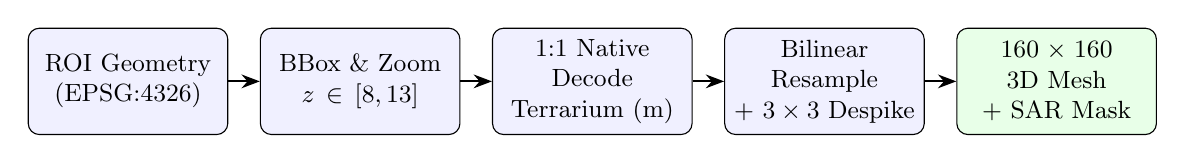
\begin{tikzpicture}[node distance=4mm,
  caja/.style={draw,rounded corners,fill=blue!6,align=center,text width=2.3cm,minimum height=1.35cm,font=\small},
  sal/.style={caja,fill=green!9},
  fl/.style={-{Stealth},thick}]
\node[caja] (a) {ROI Geometry\\(EPSG:4326)};
\node[caja,right=of a] (b) {BBox \& Zoom\\$z\in[8,13]$};
\node[caja,right=of b] (c) {1:1 Native Decode\\Terrarium (m)};
\node[caja,right=of c] (d) {Bilinear Resample\\+ $3\times3$ Despike};
\node[sal,right=of d] (e) {$160\times160$ 3D Mesh\\+ SAR Mask};
\draw[fl] (a)--(b); \draw[fl] (b)--(c); \draw[fl] (c)--(d); \draw[fl] (d)--(e);
\end{tikzpicture}
\caption{Client-side processing pipeline of the 3D Terrain Viewer (\src{web/src/utils/terrain3d.ts}).
RGB-to-meters elevation decoding occurs at native $1:1$ tile resolution prior to any spatial interpolation.}
\label{fig:flujo-relieve3d}
\end{figure}

\section{Mathematical Formulation of the Elevation Mesh}
\label{sec:relieve3d-matematicas}

\subsection{Bounding Box, Web Mercator Projection, and Zoom Selection}
\label{sec:relieve3d-mercator}

Given an active ROI geometry in WGS84 geographic coordinates ($\mathrm{EPSG}{:}4326$)---whether a \texttt{Polygon}, an administrative \texttt{MultiPolygon}, or a manually drawn coordinate ring---the function \texttt{bboxFromGeometry} extracts its geographic bounding box:
\begin{equation}
  \mathcal{B} = [\lambda_{\min},\ \varphi_{\min},\ \lambda_{\max},\ \varphi_{\max}],
  \label{eq:bbox-relieve}
\end{equation}
where $\lambda\in[-180^\circ,180^\circ]$ is longitude and $\varphi\in[-85.0511^\circ,85.0511^\circ]$ is latitude clamped to the Web Mercator ($\mathrm{EPSG}{:}3857$) domain. To prevent excessive client tile downloads, the angular span is bounded to $\Delta\lambda = \lambda_{\max}-\lambda_{\min}\le 3^\circ$ and $\Delta\varphi = \varphi_{\max}-\varphi_{\min}\le 3^\circ$.

At integer zoom level $z\in[8,13]$, the Web Mercator pyramid has $2^z$ tiles per axis. Continuous tile coordinates $(X_t,Y_t)\in[0,2^z)$ are given by the spherical Mercator transformation:
\begin{equation}
  X_t(\lambda,z) = \frac{\lambda + 180^\circ}{360^\circ}\,2^z,
  \qquad
  Y_t(\varphi,z) = \frac{1}{2}\left[
    1 - \frac{1}{\pi}\ln\!\left(\tan\!\left(\frac{\varphi\pi}{180^\circ}\right)
    + \sec\!\left(\frac{\varphi\pi}{180^\circ}\right)\right)
  \right] 2^z .
  \label{eq:mercator-tiles}
\end{equation}
The integer tile indices covering $\mathcal{B}$ are $x_0=\lfloor X_t(\lambda_{\min},z)\rfloor$, $x_1=\lfloor X_t(\lambda_{\max},z)-10^{-9}\rfloor$, $y_0=\lfloor Y_t(\varphi_{\max},z)\rfloor$, and $y_1=\lfloor Y_t(\varphi_{\min},z)-10^{-9}\rfloor$ (where $Y_t$ increases from North to South). The function \texttt{chooseZoom} selects the highest resolution level whose total tile count does not exceed the budget $N_{\max}=36$ tiles:
\begin{equation}
  z^\ast = \max\Bigl\{\, z\in\{8,9,10,11,12,13\} \;\Big|\;
  (x_1 - x_0 + 1)(y_1 - y_0 + 1) \le N_{\max} \,\Bigr\}.
  \label{eq:choose-zoom}
\end{equation}

The horizontal metric dimensions $(W_m,H_m)$ of bounding box $\mathcal{B}$---required both to preserve the true horizontal aspect ratio of the 3D block and to compute terrain slope derivatives in meters per meter---are evaluated on the mean Earth sphere of radius $R_\oplus = 6,371,008.8\,\unit{m}$ at mid-latitude $\bar\varphi = (\varphi_{\min}+\varphi_{\max})/2$:
\begin{equation}
  W_m = R_\oplus\,\frac{(\lambda_{\max}-\lambda_{\min})\pi}{180^\circ}\,\cos\!\left(\frac{\bar\varphi\pi}{180^\circ}\right),
  \qquad
  H_m = R_\oplus\,\frac{(\varphi_{\max}-\varphi_{\min})\pi}{180^\circ}.
  \label{eq:bbox-metros}
\end{equation}

\subsection{Native 1:1 Decoding of AWS Terrarium Tiles}
\label{sec:relieve3d-terrarium}

Terrain elevation is sourced from open \textbf{AWS Terrarium} tiles ($256\times256$ 8-bit RGB PNGs derived from SRTM/NASADEM and public elevation datasets). Each pixel encodes elevation in meters across its red $R$, green $G$, and blue $B$ byte channels ($R,G,B\in\{0,1,\ldots,255\}$):
\begin{equation}
  h_{\mathrm{raw}}(R,G,B) = \left(256\,R + G + \frac{B}{256}\right) - 32,768\quad[\unit{m}].
  \label{eq:terrarium-decode}
\end{equation}
In this base-256 fixed-point encoding:
\begin{itemize}
  \item Channel $R$ contributes coarse $256\,\unit{m}$ steps (with $R=128, G=0, B=0$ representing exactly $0\,\unit{m}$ sea level).
  \item Channel $G$ contributes integer meters ($0$ to $255\,\unit{m}$).
  \item Channel $B$ contributes sub-meter fractions with resolution $1/256\,\unit{m}\approx 3.9\,\unit{mm}$.
\end{itemize}

\warn{Terrarium PNG images must never be scaled or interpolated in RGB color space prior to applying Equation~\eqref{eq:terrarium-decode}. If a pixel at $h=255\,\unit{m}$ ($R=128,G=255,B=0$) and an adjacent pixel at $h=256\,\unit{m}$ ($R=129,G=0,B=0$) are linearly blended in RGB space, the intermediate pixel receives $R=128,G=128$ ($h=128\,\unit{m}$) or, if $R$ rounds up to $129$ while $G$ remains high, creates a spurious $+256\,\unit{m}$ single-vertex needle spike. To prevent this, \src{web/src/utils/terrain3d.ts} decodes each tile via \texttt{createImageBitmap(blob, \{colorSpaceConversion: 'none'\})} onto a native $1:1$ ($256\times256$) canvas with \texttt{imageSmoothingEnabled = false} and immediately converts every pixel into a metric \texttt{Float32Array}.}

\subsection{Coastal Sanitization and Bathymetry Clamping}
\label{sec:relieve3d-saneamiento}

Along coastal regions (such as the Acapulco ROI), Terrarium tiles contain deep ocean bathymetry descending to $-9,651\,\unit{m}$. Allowing negative submarine depths into the 3D terrain block would artificially inflate total relief $\Delta z$ beyond $10,000\,\unit{m}$, distorting the side walls and compressing terrestrial hypsometric colors into a flat uniform hue.

The function \texttt{sanitizeElevationSample} verifies full alpha opacity ($\alpha=255$), rejects corrupted values above the physical ceiling $h_{\mathrm{ceil}}=9,000\,\unit{m}$, and clamps negative elevations to sea level $h_{\mathrm{floor}}=0\,\unit{m}$:
\begin{equation}
  h_{\mathrm{san}}(R,G,B,\alpha) =
  \begin{cases}
    \mathrm{NaN}, & \text{if } \alpha < 255 \;\vee\; \neg\text{finite}(h_{\mathrm{raw}}) \;\vee\; h_{\mathrm{raw}} > 9,000\,\unit{m},\\[4pt]
    \max\bigl(0\,\unit{m},\ h_{\mathrm{raw}}(R,G,B)\bigr), & \text{otherwise.}
  \end{cases}
  \label{eq:saneamiento-costero}
\end{equation}
Thus, ocean surfaces render flat at $0\,\unit{m}$ and reported minimum/maximum elevations reflect exclusively emergent land within the ROI.

\subsection{Bilinear Resampling in Meters onto the \texorpdfstring{$161\times161$}{161x161} Mesh}
\label{sec:relieve3d-bilineal}

Once the native sanitized elevation mosaic $M(x,y)$ in meters ($W_s\times H_s$ pixels) is assembled, the continuous sub-window $[s_x, s_x+s_w]\times[s_y, s_y+s_h]$ matching bounding box $\mathcal{B}$ is resampled onto the 3D mesh grid of $N_c\times N_r = 161\times161$ vertices ($160\times160$ segments).

For each vertex $(c,r)$ with $c\in\{0,\ldots,N_c-1\}$ and $r\in\{0,\ldots,N_r-1\}$, the continuous source mosaic coordinates are:
\begin{equation}
  f_x = s_x + \frac{c}{N_c - 1}\,s_w,
  \qquad
  f_y = s_y + \frac{r}{N_r - 1}\,s_h,
\end{equation}
with base indices $x_0=\lfloor f_x\rfloor$, $y_0=\lfloor f_y\rfloor$, $x_1=\min(W_s-1,x_0+1)$, $y_1=\min(H_s-1,y_0+1)$ and fractional weights $t_x = f_x - x_0$, $t_y = f_y - y_0$. When all four neighboring samples $h_{00}=M(x_0,y_0)$, $h_{10}=M(x_1,y_0)$, $h_{01}=M(x_0,y_1)$, and $h_{11}=M(x_1,y_1)$ are finite, \texttt{resampleElevationBilinear} evaluates bilinear interpolation directly in meters:
\begin{equation}
  h(c,r) = (1 - t_y)\bigl[(1 - t_x)h_{00} + t_x h_{10}\bigr]
         + t_y\bigl[(1 - t_x)h_{01} + t_x h_{11}\bigr].
  \label{eq:bilineal-metros}
\end{equation}
If any neighbor is $\mathrm{NaN}$, the function falls back to the average of available finite neighbors in the $2\times2$ cell.

\subsection{Conditional \texorpdfstring{$3\times3$}{3x3} Anti-Spike Filter (\texttt{despikeElevationGrid})}
\label{sec:relieve3d-despike}

Even under native $1:1$ decoding, an upstream tile may occasionally contain an isolated corrupted pixel. To suppress single-vertex needle spikes without blunting genuine canyon rims or mountain ridges, \texttt{despikeElevationGrid} applies a conditional median filter over the punctured 8-neighbor ring $\mathcal{N}_{3\times3}(c,r)$:
\begin{equation}
  \mathcal{N}_{3\times3}(c,r) = \Bigl\{\, h(c+\delta_c,\ r+\delta_r) \;\Big|\;
  \delta_c,\delta_r\in\{-1,0,1\},\ (\delta_c,\delta_r)\neq(0,0) \,\Bigr\}.
\end{equation}
Let $m_{c,r} = \operatorname{median}\bigl(\mathcal{N}_{3\times3}(c,r)\bigr)$ denote the median of the finite neighbors. Using a single-step spike threshold $\tau_{\mathrm{spike}} = 80\,\unit{m}$, the filtered elevation $\tilde{h}(c,r)$ is:
\begin{equation}
  \tilde{h}(c,r) =
  \begin{cases}
    m_{c,r}, & \text{if } \bigl|h(c,r) - m_{c,r}\bigr| > \tau_{\mathrm{spike}} \;\vee\; \neg\text{finite}\bigl(h(c,r)\bigr),\\[4pt]
    h(c,r), & \text{otherwise.}
  \end{cases}
  \label{eq:despike}
\end{equation}
On a real continuous slope (e.g., inside Sumidero Canyon), the 8 neighbors bracket the central value symmetrically, so $|h(c,r)-m_{c,r}|\approx 0$ and the true slope remains untouched. Conversely, an isolated $+256\,\unit{m}$ byte-jump spike exceeds $\tau_{\mathrm{spike}}=80\,\unit{m}$ and is cleanly replaced by $m_{c,r}$.

Final ROI relief telemetry metrics are evaluated after despiking:
\begin{equation}
  h_{\min} = \min_{c,r} \tilde{h}(c,r),
  \qquad
  h_{\max} = \max_{c,r} \tilde{h}(c,r),
  \qquad
  \Delta z = h_{\max} - h_{\min}.
  \label{eq:telemetria-relieve}
\end{equation}

\begin{ejemplo}[Effect of the Anti-Spike Filter on a Slope with a $+256\,\unit{m}$ Needle]
Consider a $3\times3$ subgrid on a uniform planar slope rising $20\,\unit{m}$ per column Eastward and $15\,\unit{m}$ per row Southward, centered at $570\,\unit{m}$. The 8 neighbors have elevations $\{535, 555, 575, 550, 590, 565, 585, 605\}\,\unit{m}$, whose sorted median is $m = 0.5\times(565+575) = 570\,\unit{m}$. If the central vertex suffers a $+256\,\unit{m}$ red-channel byte jump to $570 + 256 = 826\,\unit{m}$, its deviation from the neighborhood median is $|826 - 570| = 256\,\unit{m} > 80\,\unit{m}$. Equation~\eqref{eq:despike} restores the center vertex to $570\,\unit{m}$ without altering a single millimeter of the surrounding slope (verified in \src{web/tests/terrain3d.test.mjs}).
\end{ejemplo}

\subsection{3D Block Geometry, Vertical Exaggeration, and Slate Pedestal}
\label{sec:relieve3d-bloque}

In the Three.js scene (\src{web/src/components/Terrain3DViewer.tsx}), the longer horizontal side of the ROI is normalized to $L_0 = 100$ scene units via the metric scale factor:
\begin{equation}
  k = \frac{L_0}{\max(W_m,\ H_m,\ 1\,\unit{m})},
  \qquad
  W = k\,W_m,
  \qquad
  H = k\,H_m.
  \label{eq:escala-escena}
\end{equation}
Given the user-controlled vertical exaggeration factor $E_v \in [1.0, 5.0]$ (defaulting to $E_v = 2.0$), the vertical displacement of each \texttt{PlaneGeometry} vertex above the ROI base elevation is:
\begin{equation}
  Z(c,r) = k\,E_v\,\bigl(\tilde{h}(c,r) - h_{\min}\bigr) \ge 0.
  \label{eq:z-vertice}
\end{equation}
To give the model a clean architectural cross-section appearance rather than a bulky cube, the four side walls and bottom plate (rendered in dark slate \texttt{\#334155} and \texttt{\#1e293b}) extend to a fixed pedestal depth equal to $3.5\,\text{\%}$ of the longer horizontal dimension, independent of $E_v$:
\begin{equation}
  Z_{\mathrm{base}} = -0.035\,\max(W, H).
  \label{eq:zocalo-fijo}
\end{equation}

\begin{figure}[htbp]
  \centering
  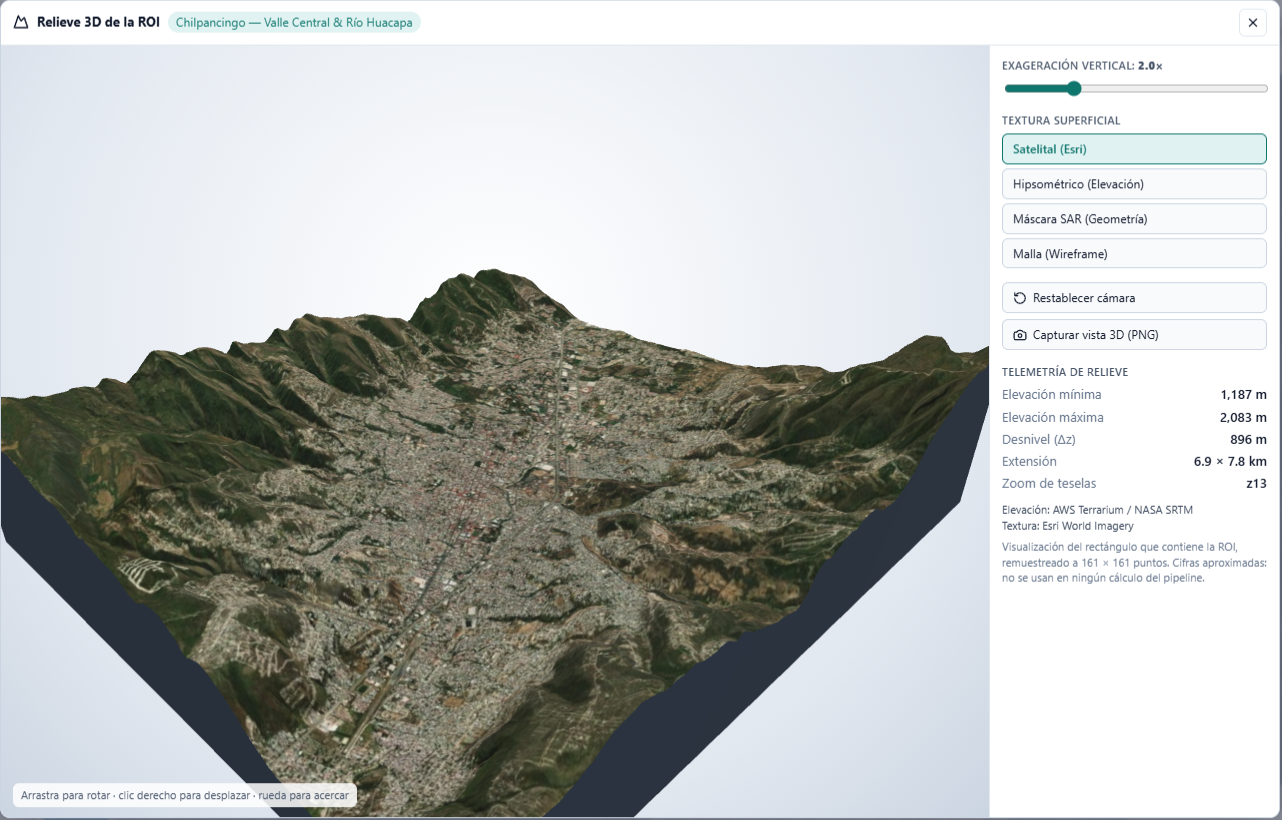
\includegraphics[width=0.82\textwidth]{fig/IMG_visor_3d_satelital.png}
  \caption{Interactive 3D topographic block model in \texttt{Terrain3DViewer} with \emph{Satellite (Esri World Imagery)} texture, $2.0\times$ vertical exaggeration, thin dark-slate pedestal, and right-hand controls and telemetry sidebar ($\Delta z$, $h_{\min}$, $h_{\max}$, extent, and tile zoom).}
  \label{fig:visor-3d-satelital}
\end{figure}

\subsection{Lambertian Directional Hillshading (Hypsometric Mode)}
\label{sec:relieve3d-hillshade}

When the user selects \textbf{Hypsometric (Elevation)} texture mode, \texttt{hypsometricCanvas} blends an altitudinal color ramp with analytical Lambertian hillshading. Let $t = (\tilde{h} - h_{\min})/\max(h_{\max}-h_{\min},1)\in[0,1]$ denote normalized elevation:
\begin{itemize}
  \item If the ROI reaches sea level ($h_{\min}\le 0.5\,\unit{m}$) and a vertex satisfies $\tilde{h}(c,r)\le 0.5\,\unit{m}$, it is assigned a constant coastal blue $\mathrm{RGB}=(38,118,178)$ without slope shading.
  \item For emergent terrain, color is piecewise linearly interpolated across lowland green $(38,115,77)$ at $t=0$, light green $(110,168,88)$ at $t=0.20$, mid-slope ochre $(224,206,128)$ at $t=0.45$, montane brown $(166,112,68)$ at $t=0.72$, alpine rock gray $(132,108,94)$ at $t=0.90$, and summit white $(245,245,245)$ at $t=1.0$.
\end{itemize}
With horizontal grid spacings $\Delta x = W_m/(N_c-1)$ and $\Delta y = H_m/(N_r-1)$, centered finite-difference gradients scaled by visual enhancement factor $f_z = 2.2$ are:
\begin{equation}
  p = f_z\,\frac{\tilde{h}(c+1,r) - \tilde{h}(c-1,r)}{2\,\Delta x},
  \qquad
  q = f_z\,\frac{\tilde{h}(c,r-1) - \tilde{h}(c,r+1)}{2\,\Delta y},
  \label{eq:grad-hillshade}
\end{equation}
where $x$ increases Eastward and $y$ increases Northward (while row index $r$ increases Southward). Illuminating from the Northwest (azimuth $315^\circ$, elevation $42^\circ$) with unit light vector $\hat{\mathbf{s}} = (-0.526,\ 0.526,\ 0.669)$, the dot product with unit surface normal $\hat{\mathbf{n}} = (-p,-q,1)/\sqrt{p^2+q^2+1}$ modulates each RGB channel $C\in\{R,G,B\}$ via:
\begin{equation}
  \cos\gamma = \frac{-p\,s_x - q\,s_y + s_z}{\sqrt{p^2 + q^2 + 1}},
  \qquad
  S = \operatorname{clip}\!\bigl(0.45 + 0.85\max(0,\cos\gamma),\ 0.48,\ 1.22\bigr),
  \qquad
  C_{\mathrm{out}} = \min\bigl(255,\ \operatorname{round}(C\cdot S)\bigr).
  \label{eq:lambert-hillshade}
\end{equation}

\begin{figure}[htbp]
  \centering
  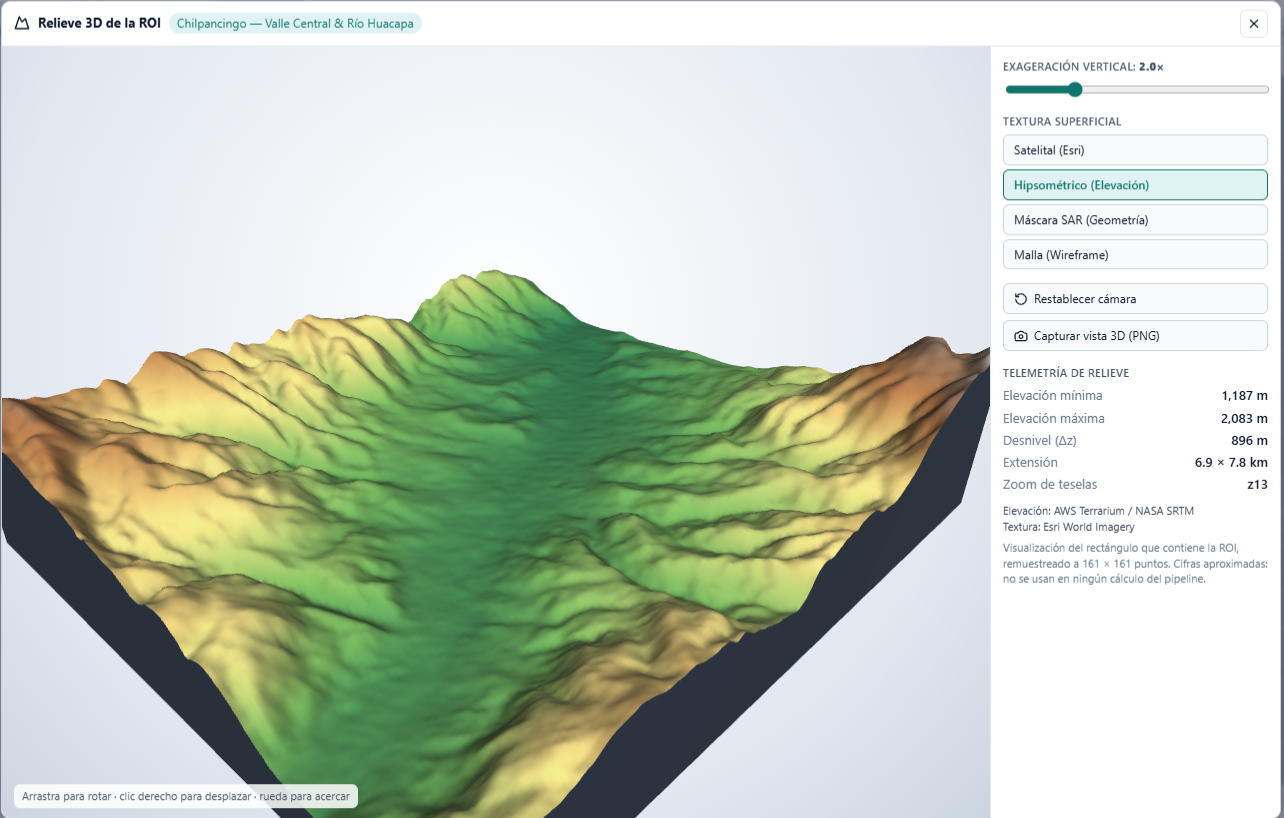
\includegraphics[width=0.82\textwidth]{fig/IMG_visor_3d_hipsometrico.png}
  \caption{The same ROI rendered in \emph{Hypsometric (Elevation)} mode inside the 3D viewer. Coastal blue delineates $0\,\unit{m}$ water bodies, while the elevation color ramp and Lambertian hillshading~\eqref{eq:lambert-hillshade} highlight watershed divides and canyon walls.}
  \label{fig:visor-3d-hipsometrico}
\end{figure}

\section{3D SAR Geometric Feasibility Mask: Critical Slope, Layover, and Shadow}
\label{sec:relieve3d-mascara-sar}

As explained in Section~\ref{sec:gcov}, NISAR GCOV products apply Radiometric Terrain Correction (RTC) to normalize illuminated area, but current catalog releases set \texttt{shadowMaskingApplied = False}: pixels compromised by topographic inversion (\emph{layover}) or beam occlusion (radar shadow) are not flagged in the product \texttt{mask} layer. The 3D viewer's \textbf{SAR Mask (Geometry)} texture mode computes and drapes directly onto the 3D terrain mesh a diagnostic map showing where radar backscatter measurements are geometrically reliable and where severe relief distortions dominate.

\begin{intuicion}
Imagine illuminating a 3D mountain scale model with a flashlight held to one side at $43^\circ$ from the vertical (NISAR's nominal incidence angle $\theta_i$):
\begin{itemize}
  \item Over \textbf{gentle valleys and plains} ($\alpha \le 15^\circ$), the beam illuminates the ground smoothly: temporal backscatter changes ($\Delta\gamma^0$) reliably reflect surface changes.
  \item On \textbf{steep cliffs facing directly toward the flashlight} at slopes $\ge 43^\circ$, the mountain crest lies closer to the flashlight than the cliff base. Echoes from the summit and base arrive simultaneously mixed together: this is \textbf{\emph{layover}} (mapped in red).
  \item On \textbf{steep back-slopes facing away from the flashlight} at angles steeper than the grazing ray ($90^\circ - 43^\circ = 47^\circ$), the beam skims right over the ridge crest leaving the lee slope in darkness: this is \textbf{radar shadow} (mapped in deep indigo).
\end{itemize}
When the satellite switches from an Ascending orbit (illuminating from East to West) to a Descending orbit (illuminating from West to East), cliffs that were in \emph{layover} flip into radar shadow and vice versa.
\end{intuicion}

\subsection{NISAR Left-Looking Side-Incidence Geometry}
\label{sec:relieve3d-geometria-nisar}

Unlike right-looking SAR missions, NISAR's L-band radar is \textbf{left-looking} (\texttt{lookDirection = Left}):
\begin{itemize}
  \item \textbf{Ascending Orbit (e.g., stack T62/F10):} the spacecraft flies South-to-North along a heading of $\approx 350^\circ$ (tilted slightly West by orbital inclination). Looking $90^\circ$ to its left, the radar pulse propagates from the satellite toward the ground along horizontal azimuth $\psi_{\mathrm{asc}} \approx 260^\circ$ (West-Southwest).
  \item \textbf{Descending Orbit (e.g., stack T55/F80):} the spacecraft flies North-to-South along a heading of $\approx 190^\circ$. Looking $90^\circ$ to its left, the radar pulse propagates from the satellite toward the ground along horizontal azimuth $\psi_{\mathrm{desc}} \approx 100^\circ$ (East-Southeast).
\end{itemize}

Letting $\psi \in \{260^\circ, 100^\circ\}$ denote the horizontal beam propagation azimuth measured clockwise from North, the horizontal unit look vector in local East--North coordinates is:
\begin{equation}
  \hat{\mathbf{l}}_{\mathrm{h}} = (l_x,\ l_y) = \left(\sin\psi,\ \cos\psi\right).
  \label{eq:vector-haz-sar}
\end{equation}

\subsection{True Metric Terrain Derivatives and Radar-Projected Slope}
\label{sec:relieve3d-ecuaciones-sar}

At every vertex $(c,r)$ of the despiked elevation grid $\tilde{h}$, \texttt{computeSarGeometricMask} evaluates the true physical partial derivatives (unexaggerated, in dimensionless $\unit{m/m}$) via centered finite differences in the interior and one-sided differences along the boundary edges:
\begin{equation}
  z_x(c,r) = \frac{\partial \tilde{h}}{\partial x}
  \approx \frac{\tilde{h}(c_{\mathrm{next}},r) - \tilde{h}(c_{\mathrm{prev}},r)}{(c_{\mathrm{next}} - c_{\mathrm{prev}})\,\Delta x},
  \qquad
  z_y(c,r) = \frac{\partial \tilde{h}}{\partial y}
  \approx \frac{\tilde{h}(c,r_{\mathrm{prev}}) - \tilde{h}(c,r_{\mathrm{next}})}{(r_{\mathrm{next}} - r_{\mathrm{prev}})\,\Delta y}.
  \label{eq:derivadas-reales-sar}
\end{equation}
From $(z_x, z_y)$, two fundamental geometric quantities are derived:
\begin{enumerate}
  \item \textbf{True topographic slope magnitude $\alpha$:}
        \begin{equation}
          \tan\alpha(c,r) = \sqrt{z_x^2(c,r) + z_y^2(c,r)},
          \qquad
          \alpha(c,r) = \arctan\sqrt{z_x^2(c,r) + z_y^2(c,r)}.
          \label{eq:pendiente-real}
        \end{equation}
  \item \textbf{Directional slope projected along the radar beam propagation vector ($s_{\mathrm{rad}}$):}
        \begin{equation}
          s_{\mathrm{rad}}(c,r) = \nabla\tilde{h}(c,r)\cdot\hat{\mathbf{l}}_{\mathrm{h}}
          = z_x(c,r)\,l_x + z_y(c,r)\,l_y,
          \qquad
          \alpha_{\mathrm{rad}}(c,r) = \arctan\bigl(s_{\mathrm{rad}}(c,r)\bigr).
          \label{eq:pendiente-proyectada}
        \end{equation}
\end{enumerate}

The sign of $s_{\mathrm{rad}}$ carries direct physical meaning:
\begin{itemize}
  \item When $s_{\mathrm{rad}} > 0$, terrain elevation \emph{rises} along the advancing radar wave direction $\hat{\mathbf{l}}_{\mathrm{h}}$---meaning the slope \textbf{faces toward the incoming radar beam}.
  \item When $s_{\mathrm{rad}} < 0$, terrain elevation \emph{drops} along the advancing wave direction---meaning the slope \textbf{faces away from the incoming radar beam}.
\end{itemize}

\subsection{Four-Class Classification Thresholds}
\label{sec:relieve3d-clases-sar}

Using nominal incidence angle $\theta_i = 43^\circ$ (representative of the Chiapas ROI swath where $\theta_i\in[42.3^\circ,45.4^\circ]$, Figure~E in Section~\ref{sec:figuras}) and critical slope threshold $\alpha_c = 15^\circ$, each vertex $(c,r)$ is classified in strict priority order:
\begin{equation}
  \mathrm{Class}(c,r) =
  \begin{cases}
    \text{\textbf{Layover / severe foreshortening}}, &
      \text{if } s_{\mathrm{rad}}(c,r) \ge \tan\theta_i
      \quad\bigl(\alpha_{\mathrm{rad}} \ge \theta_i\bigr),\\[6pt]
    \text{\textbf{Radar shadow}}, &
      \text{if } -s_{\mathrm{rad}}(c,r) \ge \tan(90^\circ - \theta_i)
      \quad\bigl(-\alpha_{\mathrm{rad}} \ge 90^\circ - \theta_i\bigr),\\[6pt]
    \text{\textbf{Critical slope}}, &
      \text{if } \sqrt{z_x^2 + z_y^2} > \tan\alpha_c
      \quad\bigl(\alpha > 15^\circ\text{ without layover or shadow}\bigr),\\[6pt]
    \text{\textbf{Reliable}}, &
      \text{otherwise} \quad\bigl(\alpha \le 15^\circ\text{ without layover or shadow}\bigr).
  \end{cases}
  \label{eq:clasificacion-sar}
\end{equation}

For $\theta_i = 43^\circ$ and $\alpha_c = 15^\circ$, the three dimensionless slope thresholds evaluate to:
\begin{equation}
  \tan 15^\circ \approx 0.2679,
  \qquad
  \tan 43^\circ \approx 0.9325,
  \qquad
  \tan(90^\circ - 43^\circ) = \tan 47^\circ \approx 1.0724.
\end{equation}

\begin{table}[htbp]
\centering\small
\begin{tabularx}{\linewidth}{p{.23\linewidth}p{.16\linewidth}p{.24\linewidth}X}
\toprule
\textbf{Category} & \textbf{Color} & \textbf{Geometric Condition} & \textbf{Implication for Interpreting $\Delta\gamma^0$}\\\midrule
Reliable & Green \texttt{\#22C55E} & $\alpha \le 15^\circ$, no layover/shadow & Stable viewing geometry; optimal terrain for quantifying soil moisture, flood, or vegetation change.\\
Critical slope & Amber \texttt{\#F59E0B} & $\alpha > 15^\circ$, no layover/shadow & Moderate foreshortening; RTC area normalization operates near DEM resolution limits.\\
Layover / foreshortening & Red \texttt{\#EF4444} & $s_{\mathrm{rad}} \ge \tan\theta_i$ & Topographic folding mixing crest and base echoes; do not interpret pixel-level $\Delta\gamma^0$.\\
Radar shadow & Indigo \texttt{\#1E1B4B} & $-s_{\mathrm{rad}} \ge \tan(90^\circ-\theta_i)$ & Occluded lee slope receiving no direct beam energy; dominated by receiver thermal noise.\\\bottomrule
\end{tabularx}
\caption{SAR geometric feasibility mask categories in the 3D Terrain Viewer (\texttt{computeSarGeometricMask}).}
\label{tab:clases-mascara-sar}
\end{table}

Across all $N_{\mathrm{tot}} = N_c N_r = 25,921$ mesh vertices, the percentage of ROI area in each geometric regime is reported in the live telemetry sidebar:
\begin{equation}
  P_k = 100\,\frac{N_k}{N_{\mathrm{tot}}}\,\mathrm{\%},
  \qquad
  k \in \{\text{reliable},\ \text{critical},\ \text{layover},\ \text{shadow}\},
  \qquad
  \sum_k P_k = 100\,\mathrm{\%}.
  \label{eq:porcentajes-sar}
\end{equation}

\begin{ejemplo}[Layover-to-Shadow Inversion When Switching Orbits on a Canyon Wall]
Consider a steep canyon wall in Sumidero Canyon rising Westward at a constant gradient of $+200\,\unit{m}$ per $100\,\unit{m}$ horizontal distance ($z_x = -2.0$, $z_y = 0$, i.e., $\alpha = \arctan(2.0) = 63.4^\circ$):
\begin{itemize}
  \item \textbf{In Ascending Orbit ($\psi = 260^\circ$):} $l_x = \sin 260^\circ = -0.9848$. The radar-projected slope is $s_{\mathrm{rad}} = (-2.0)(-0.9848) = +1.9696$. Since $1.9696 \ge \tan 43^\circ = 0.9325$, the entire cliff is classified as \textbf{Layover} ($100\,\mathrm{\%}$).
  \item \textbf{In Descending Orbit ($\psi = 100^\circ$):} $l_x = \sin 100^\circ = +0.9848$. Now the radar-projected slope reverses sign to $s_{\mathrm{rad}} = (-2.0)(+0.9848) = -1.9696$. Since $-s_{\mathrm{rad}} = 1.9696 \ge \tan 47^\circ = 1.0724$, the exact same canyon wall flips completely into \textbf{Radar Shadow} ($100\,\mathrm{\%}$).
\end{itemize}
This explains why the 3D viewer provides a live toggle between \emph{Ascending (T62/F10)} and \emph{Descending (T55/F80)}, and visually demonstrates why opposite orbital passes must never be mixed in a $\Delta\gamma^0$ difference map.
\end{ejemplo}

\begin{figure}[htbp]
  \centering
  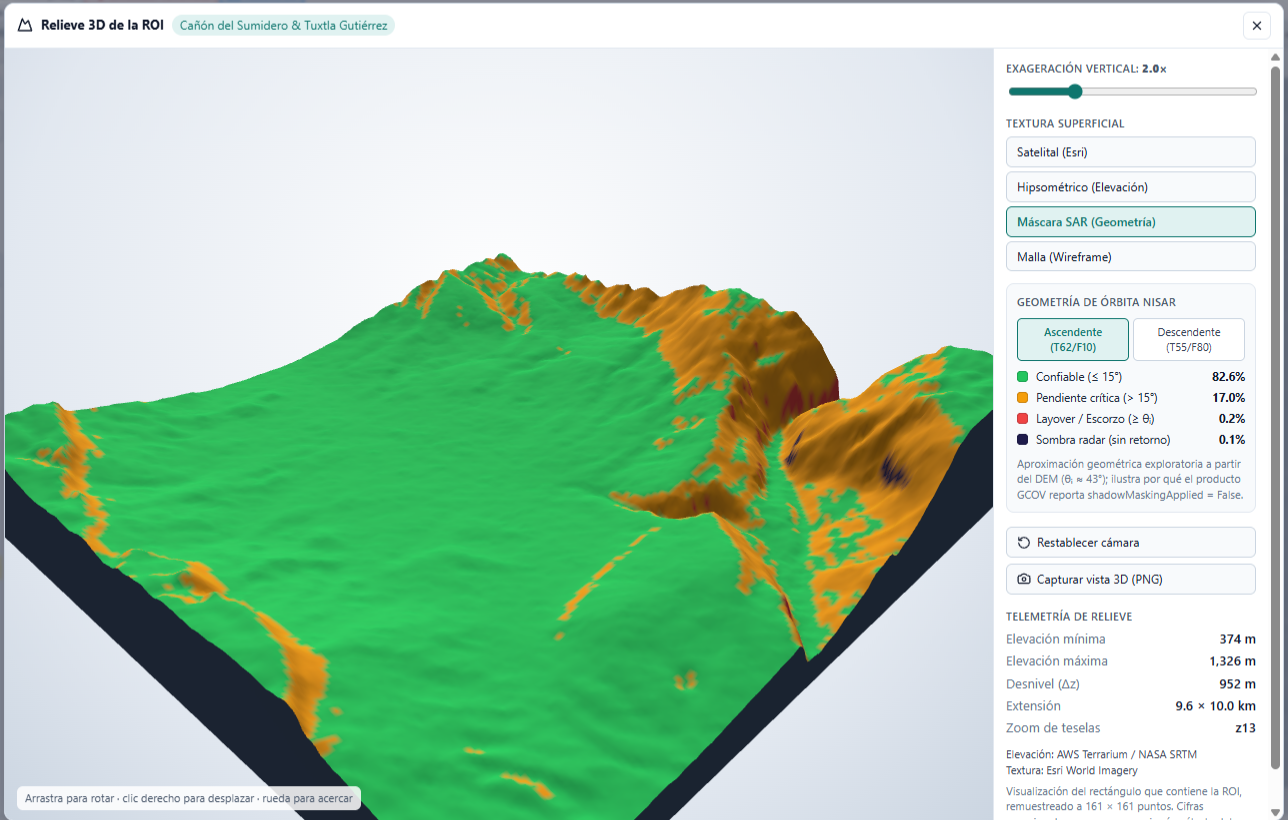
\includegraphics[width=0.82\textwidth]{fig/IMG_visor_3d_mascara_sar_asc.png}
  \caption{\emph{SAR Mask (Geometry)} mode draped over the 3D terrain block for the \textbf{Ascending (T62/F10)} pass.
  Green delineates reliable valleys and plains ($\alpha\le 15^\circ$), amber marks critical slopes ($>15^\circ$), and red/indigo highlight canyon walls affected by \emph{layover} and radar shadow.}
  \label{fig:visor-3d-sar-asc}
\end{figure}

\begin{figure}[htbp]
  \centering
  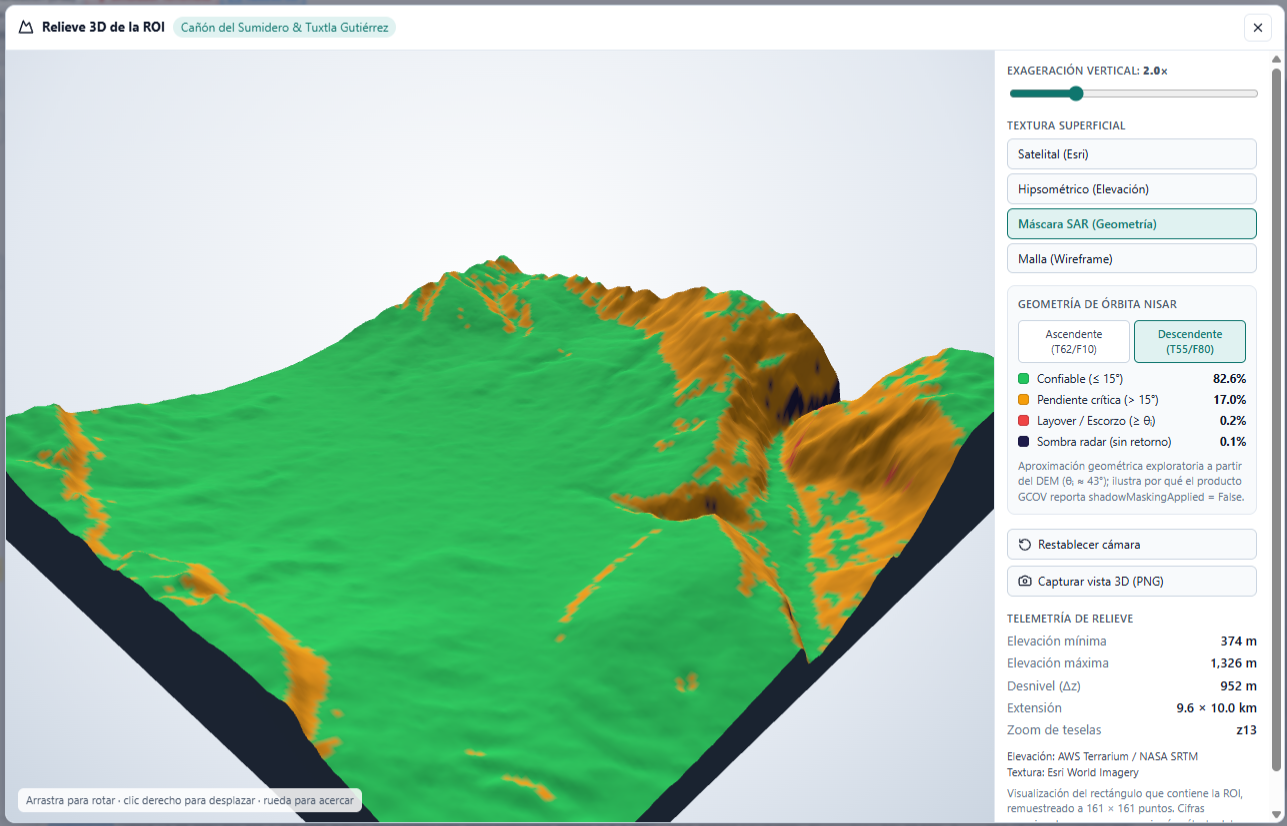
\includegraphics[width=0.82\textwidth]{fig/IMG_visor_3d_mascara_sar_desc.png}
  \caption{Geometric inversion upon toggling to the \textbf{Descending (T55/F80)} pass in the 3D viewer sidebar. East/West-facing canyon walls swap their \emph{layover} (red) and radar shadow (deep indigo) regimes, updating class percentages in real time.}
  \label{fig:visor-3d-sar-desc}
\end{figure}

\section{WebGL Memory Management and Module Verification}
\label{sec:relieve3d-webgl}

To ensure that repeatedly opening and closing the 3D modal never leaks GPU memory or exhausts browser WebGL contexts needed by MapLibre GL, \texttt{Terrain3DViewer} executes a deterministic teardown sequence on unmount:
\begin{enumerate}
  \item Cancels the animation frame loop (\texttt{cancelAnimationFrame}) and disconnects the \texttt{ResizeObserver}.
  \item Disposes the \texttt{OrbitControls} instance (\texttt{controls.dispose()}).
  \item Explicitly disposes all GPU buffers across the three geometries (\texttt{surfaceGeom}, \texttt{wallGeom}, \texttt{bottomGeom}), four materials (\texttt{surfaceMat}, \texttt{wireMat}, \texttt{wallMat}, \texttt{bottomMat}), and all allocated \texttt{CanvasTexture} instances.
  \item Invokes \texttt{renderer.dispose()}, forces native WebGL context release via \texttt{renderer.forceContextLoss()}, and removes the \texttt{<canvas>} element from the DOM.
\end{enumerate}

The automated test suite \src{web/tests/terrain3d.test.mjs} independently verifies native Terrarium decoding~\eqref{eq:terrarium-decode}, bounding-box extraction, Web Mercator tile selection~\eqref{eq:mercator-tiles}, coastal sanitization~\eqref{eq:saneamiento-costero}, $+256\,\unit{m}$ spike removal~\eqref{eq:despike} without slope distortion, SAR geometric classification~\eqref{eq:clasificacion-sar} across flat plains and cliffs for both orbital passes, ES/EN i18n completeness, and WebGL teardown calls.

\clearpage
\part{Seismic Simulator, GMPE Attenuation, P/S Wavefronts, and Signal Processing}
\label{part:sismo}

This part documents the physical-mathematical and digital signal processing engine of the TerraPulse AI seismic
simulation module (\src{web/src/utils/seismic.ts}, \src{web/src/utils/signal.ts},
\src{web/src/utils/accelerogram.ts}, and associated components in \src{web/src/components/}). The module enables
formulating seismic scenarios within Mexico's tectonic regime, evaluating peak ground acceleration
($\mathrm{PGA}$) attenuation using published regional empirical laws, projecting geodesic Modified Mercalli
Intensity ($\mathrm{MMI}$) rings and 2D $P$ and $S$ wavefronts on MapLibre GL, synthesizing a $50\,\unit{Hz}$
accelerogram $a(t)$ for any receiving station, and analyzing its energetic and spectral content through Arias
Intensity ($I_A$), significant duration ($D_{5\text{--}95}$), the Fast Fourier Transform (FFT), and the
Short-Time Fourier Transform (STFT) spectrogram.

\begin{atencion}
Just like the hydraulic and solar simulators, the seismic module belongs strictly to the third epistemic tier of
Table~\ref{tab:niveles} (\emph{prediction / exploratory scenario}). It does not process SAR interferometry (GUNW
products) nor replace instrumental networks (SSN, SASMEX, RACM) or a site-specific probabilistic seismic hazard
assessment (PSHA). Figures produced for historical presets represent the median response of the analytical model
under stated assumptions, never observed measurements.
\end{atencion}

\section{Module Architecture and Computational Chain}
\label{sec:sismo-arquitectura}

The engine executes entirely in the browser with zero server latency, maintaining an isolated state per active
workspace map (\texttt{SeismicSimulationState} in \src{web/src/types/workspace.ts} and
\src{web/src/utils/seismicScenario.ts}). Figure~\ref{fig:flujo-sismo} summarizes the five-stage sequence
from source definition to spectral analysis.

\begin{figure}[htbp]
\centering
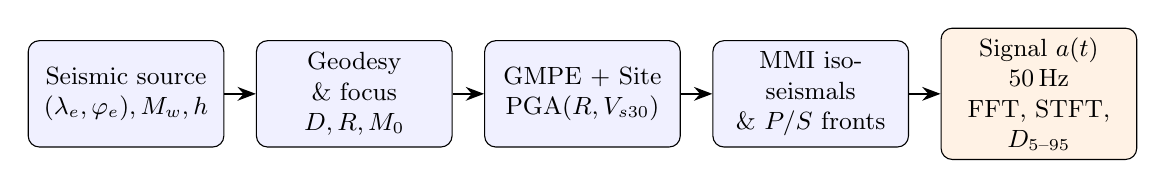
\begin{tikzpicture}[node distance=4mm,
  caja/.style={draw,rounded corners,fill=blue!6,align=center,text width=2.25cm,minimum height=1.35cm,font=\small},
  sal/.style={caja,fill=orange!10},
  fl/.style={-{Stealth},thick}]
\node[caja] (a) {Seismic source\\$(\lambda_e,\varphi_e), M_w, h$};
\node[caja,right=of a] (b) {Geodesy \& focus\\$D, R, M_0$};
\node[caja,right=of b] (c) {GMPE + Site\\$\mathrm{PGA}(R,V_{s30})$};
\node[caja,right=of c] (d) {MMI isoseismals\\\& $P/S$ fronts};
\node[sal,right=of d] (e) {Signal $a(t)$ 50\,Hz\\FFT, STFT, $D_{5\text{--}95}$};
\draw[fl] (a)--(b); \draw[fl] (b)--(c); \draw[fl] (c)--(d); \draw[fl] (d)--(e);
\end{tikzpicture}
\caption{Client-side computational chain of the seismic simulator (\src{web/src/utils/seismic.ts} and
\src{web/src/utils/signal.ts}).}
\label{fig:flujo-sismo}
\end{figure}

\section{Source Seismology and Ground Motion Prediction Equations (GMPE)}
\label{sec:sismo-gmpe}

\subsection{Scalar Seismic Moment \texorpdfstring{$M_0$}{M0} and Moment Magnitude \texorpdfstring{$M_w$}{Mw}}
\label{sec:sismo-momento}

The physical energy released by a geological rupture is quantified by the scalar seismic moment
$M_0 = \mu A \bar{u}$, where $\mu$ is the shear modulus of the rock, $A$ is the rupture area across the fault
plane, and $\bar{u}$ is the average slip. The standard relation of Hanks and Kanamori (1979) links the
dimensionless moment magnitude $M_w$ to $M_0$ (expressed in $\unit{dyn\cdot cm}$, where
$1\,\unit{dyn\cdot cm} = 10^{-7}\,\unit{N\cdot m}$):
\begin{equation}
  M_w = \frac{2}{3}\log_{10} M_0 - 10.7
  \quad\Longleftrightarrow\quad
  M_0 = 10^{\frac{3}{2}(M_w + 10.7)}\quad[\unit{dyn\cdot cm}].
  \label{eq:momento-sismico}
\end{equation}
Because of the $3/2$ factor in the exponent, a $+1.0$ increase in $M_w$ multiplies the seismic moment by
$10^{1.5}\approx 31.62$, and a $+2.0$ unit increase multiplies it by exactly $1\,000$
(implemented in \texttt{seismicMomentDynCm}).

\subsection{Great-Circle Epicentral Distance \texorpdfstring{$D$}{D} and Hypocentral Distance \texorpdfstring{$R$}{R}}
\label{sec:sismo-distancias}

Given the epicenter $(\lambda_e,\varphi_e)$ and a receiving station or surface point $(\lambda,\varphi)$ in
geographic coordinates, the surface epicentral distance $D$ over a spherical Earth of mean radius
$R_T = 6\,371\,\unit{km}$ is computed via the haversine formula (function \texttt{haversineDistanceKm}):
\begin{equation}
  D = 2\,R_T\arcsin\sqrt{
    \sin^2\!\left(\frac{\varphi - \varphi_e}{2}\right)
    + \cos\varphi_e\cos\varphi\,\sin^2\!\left(\frac{\lambda - \lambda_e}{2}\right)
  }\quad[\unit{km}].
  \label{eq:sismo-haversine}
\end{equation}
If the rupture originates at focal depth $h$ (in $\unit{km}$), the three-dimensional hypocentral distance $R$
from the point focus to the surface station is:
\begin{equation}
  R = \sqrt{D^2 + h^2}\quad[\unit{km}].
  \label{eq:sismo-hipocentral}
\end{equation}

\subsection{Ground Motion Prediction Equations (GMPE) for Mexico}
\label{sec:sismo-modelos-gmpe}

An attenuation law or GMPE (\emph{Ground Motion Prediction Equation}) estimates median Peak Ground Acceleration
($\mathrm{PGA}$) as a function of magnitude $M_w$, source distance $R$, focal depth $h$, and tectonic mechanism.
In \src{web/src/utils/seismic.ts} (\texttt{computePga\_g}), ground acceleration at a site with average top-$30\,\unit{m}$
shear-wave velocity $V_{s30}$ is decomposed into the reference firm-rock prediction plus a logarithmic site
amplification term $S_{\mathrm{site}}(V_{s30})$:
\begin{equation}
  \ln\mathrm{PGA}_{\mathrm{site}}(M_w,R,h,V_{s30})
  = \ln\mathrm{PGA}_{\mathrm{rock}}(M_w,R,h) + S_{\mathrm{site}}(V_{s30}),
  \label{eq:gmpe-general}
\end{equation}
with conversion between acceleration normalized by standard gravity ($g_0 = 980.665\,\unit{cm/s^2}$) and
CGS units ($\unit{gal} = \unit{cm/s^2}$):
\begin{equation}
  \mathrm{PGA}_{g} = \frac{\mathrm{PGA}_{\mathrm{cgs}}}{980.665\,\unit{cm/s^2}}.
\end{equation}
The simulator distinguishes Mexico's three primary seismogenic regimes:

\subsubsection*{1. Coastal Interplate Subduction: Arroyo et al.\ (2010) Model}
For interplate thrust earthquakes along the Middle America Trench (interface between the Cocos and North American
plates, from Jalisco/Colima to Chiapas), Equation~8a of Arroyo et al.\ (2010) is implemented with the
$\mathrm{PGA}$ row coefficients from their Table~2 for rock sites (NEHRP Class B, function
\texttt{pgaRockArroyo2010\_cgs}):
\begin{equation}
  \ln\mathrm{PGA}_{\mathrm{rock,cgs}}
  = \alpha_1 + \alpha_2 M_w + \alpha_3\ln\!\left[
    \frac{E_1(\alpha_4 R) - E_1\!\left(\alpha_4\sqrt{R^2 + r_0^2}\right)}{r_0^2}
  \right],
  \qquad
  r_0^2 = 1.4447\times 10^{-5}\,e^{2.3026\,M_w},
  \label{eq:gmpe-arroyo}
\end{equation}
where $\mathrm{PGA}_{\mathrm{rock,cgs}}$ is in $\unit{cm/s^2}$, the coefficients calibrated from Mexican forearc
strong-motion recordings are
\[
  \alpha_1 = 2.4862,\qquad
  \alpha_2 = 0.9392,\qquad
  \alpha_3 = 0.5061,\qquad
  \alpha_4 = 0.0150\,\unit{km^{-1}},
\]
with published natural-log standard deviation $\sigma_{\ln\mathrm{PGA}} = 0.75$, and $E_1(x)$ is the first-order
exponential integral:
\begin{equation}
  E_1(x) = \int_x^\infty \frac{e^{-u}}{u}\,\dd u, \qquad x > 0.
  \label{eq:integral-exponencial}
\end{equation}
In \texttt{exponentialIntegralE1}, $E_1(x)$ is evaluated in double precision via its power series expansion for
$x\le 1$ ($E_1(x) = -\gamma_E - \ln x - \sum_{k=1}^\infty (-x)^k/(k\cdot k!)$) and via Lentz's continued-fraction
algorithm for $x>1$ (Abramowitz \& Stegun, 1972). Physically, the difference quotient involving $E_1$ integrates
high-frequency radiation across a finite circular rupture of equivalent radius $r_0(M_w)$, naturally producing
\emph{near-field saturation} without letting acceleration diverge at small $R$.

\subsubsection*{2. Intermediate-Depth Intraslab: Garc\'ia et al.\ (2005) Model}
For normal-faulting earthquakes inside the subducted Cocos slab (\emph{inslab}, typical focal depths of $35$ to
$138\,\unit{km}$ beneath Puebla, Morelos, Oaxaca, Guerrero, and Chiapas), Equation~2 of Garc\'ia et al.\ (2005)
is implemented for the horizontal component of rock $\mathrm{PGA}$ (Table~2 of the paper, function
\texttt{pgaRockGarcia2005\_cgs}):
\begin{equation}
  \log_{10}\mathrm{PGA}_{\mathrm{rock,cgs}}
  = -0.2 + 0.59\,M_w - 0.0039\,R' - \log_{10} R' + 0.008\,h,
  \label{eq:gmpe-garcia}
\end{equation}
where $h$ is focal depth in $\unit{km}$ and $R'$ incorporates the near-source saturation term $\Delta(M_w)$ of
Atkinson and Boore (2003):
\begin{equation}
  R' = \sqrt{R^2 + \Delta^2},
  \qquad
  \Delta = 0.00750\times 10^{0.507\,M_w}\quad[\unit{km}].
  \label{eq:saturacion-garcia}
\end{equation}
The published base-10 standard deviation of the model is $\sigma_{\log_{10}\mathrm{PGA}} = 0.28$, which in
natural logarithm equals $\sigma_{\ln\mathrm{PGA}} = 0.28\ln 10 \approx 0.645$. The $+0.008\,h$ term reflects a
well-documented physical property of Mexican intraslab earthquakes: at equal magnitude and distance, deeper slab
ruptures exhibit higher stress drops and radiate stronger high-frequency ground accelerations than shallow
interplate events.

\subsubsection*{3. Shallow Crustal: Parametric Formulation with Near-Source Saturation}
For shallow crustal or transform faults (such as the San Andreas--Laguna Salada system in Baja California or
Trans-Mexican Volcanic Belt faults), a regional parametric model with the effective saturation depth
$h_{\mathrm{sat}}(M_w)$ of Yenier and Atkinson (2015) is employed (\texttt{MANUAL\_CRUSTAL\_COEFFICIENTS} and
\texttt{nearSourceSaturationKm}):
\begin{equation}
  \ln\mathrm{PGA}_{\mathrm{rock},g}
  = c_1 + c_2 M_w - c_3\ln R_{\mathrm{ef}} - c_4 R_{\mathrm{ef}},
  \qquad
  R_{\mathrm{ef}} = \sqrt{R^2 + h_{\mathrm{sat}}^2},
  \qquad
  h_{\mathrm{sat}} = 10^{-0.405 + 0.235\,M_w}\quad[\unit{km}],
  \label{eq:gmpe-cortical}
\end{equation}
with $c_1 = -1.95$, $c_2 = 0.88$, $c_3 = 1.05$, and $c_4 = 0.0028\,\unit{km^{-1}}$ (explicitly labeled in the UI
as a provisional crustal model). Across all three mechanisms, a numerical safeguard clamps
$\mathrm{PGA}_g \in [10^{-4},\ 2.5]\,g$.

\subsection{Site Amplification (\texorpdfstring{$V_{s30}$}{Vs30}) and Modified Mercalli Intensity (MMI)}
\label{sec:sismo-vs30-mmi}

The time-averaged shear-wave velocity in the upper $30\,\unit{m}$ of the subsurface, $V_{s30}$ (in
$\unit{m/s}$), parameterizes the seismic impedance of the ground. When waves propagate from bedrock
($V_{\mathrm{ref}} = 760\,\unit{m/s}$) into softer sediments ($V_{s30} < 760\,\unit{m/s}$), conservation of
elastic energy flux requires vibration amplitude to increase. The logarithmic site amplification term
(\texttt{siteAmplification}) is:
\begin{equation}
  S_{\mathrm{site}}(V_{s30}) =
  \begin{cases}
    -0.45\,\ln\!\left(\dfrac{V_{s30}}{760\,\unit{m/s}}\right), & \text{if } V_{s30} < 760\,\unit{m/s},\\[8pt]
    0, & \text{if } V_{s30} \ge 760\,\unit{m/s}.
  \end{cases}
  \label{eq:amplificacion-vs30}
\end{equation}

\begin{table}[htbp]
\centering\small
\begin{tabularx}{\linewidth}{p{.28\linewidth}rrrX}
\toprule
\textbf{Geotechnical Class} & \textbf{$V_{s30}$ [m/s]} & \textbf{$S_{\mathrm{site}}$} & \textbf{Factor $e^{S_{\mathrm{site}}}$} & \textbf{Frequency $f_S$ and coda $\tau_{\mathrm{coda}}$ in $a(t)$}\\\midrule
Firm rock (\texttt{rock}) & $760$ & $0.000$ & $1.00\times$ & $f_S = 2.20\,\unit{Hz}$, $\tau_{\mathrm{coda}} = 9.0\,\unit{s}$\\
Firm / alluvial soil (\texttt{intermediate}) & $450$ & $0.236$ & $1.27\times$ & $f_S = 1.30\,\unit{Hz}$, $\tau_{\mathrm{coda}} = 14.0\,\unit{s}$\\
Soft lacustrine clay (\texttt{soft\_lacustrine}) & $100$ & $0.913$ & $2.49\times$ & $f_S = 0.52\,\unit{Hz}$ ($T_0\approx 1.9\,\unit{s}$), $\tau_{\mathrm{coda}} = 28.0\,\unit{s}$\\\bottomrule
\end{tabularx}
\caption{Comparison of $V_{s30}$ soil classes implemented in \src{web/src/utils/seismic.ts}
(\texttt{SOIL\_VS30} and \texttt{siteWaveParams}). Users may also enter any custom
$V_{s30}\in[80,1500]\,\unit{m/s}$ for both the regional scenario and the receiving station.}
\label{tab:comparacion-vs30}
\end{table}

To translate peak ground acceleration in $\unit{cm/s^2}$ into the macroscopic damage scale of Modified Mercalli
Intensity ($\mathrm{MMI}$, clamped to $[1.0, 10.5]$), \texttt{pgaToMmi} uses the continuous bilinear relation of
Wald et al.\ (1999):
\begin{equation}
  \mathrm{MMI}(\mathrm{PGA}_{\mathrm{cgs}}) =
  \begin{cases}
    2.20\log_{10}\bigl(\mathrm{PGA}_{\mathrm{cgs}}\bigr) + 1.00, &
      \text{if } \mathrm{PGA}_{\mathrm{cgs}} \le \mathrm{PGA}_\times,\\[6pt]
    3.66\log_{10}\bigl(\mathrm{PGA}_{\mathrm{cgs}}\bigr) - 1.66, &
      \text{if } \mathrm{PGA}_{\mathrm{cgs}} > \mathrm{PGA}_\times,
  \end{cases}
  \qquad
  \mathrm{PGA}_\times = 10^{2.66/1.46} \approx 66.43\,\unit{cm/s^2},
  \label{eq:wald-mmi}
\end{equation}
where $\mathrm{PGA}_\times \approx 0.0677\,g$ ($\mathrm{MMI}\approx\text{V}$) is the exact analytical intersection
of both lines, guaranteeing continuity and strict monotonicity across the entire scale.

The four geodesic impact rings rendered on the map (destructive zone $\ge 0.34\,g$, severe damage $\ge 0.12\,g$,
strong shaking $\ge 0.03\,g$, and weak perception $\ge 0.005\,g$) are obtained by numerically inverting the
monotonically decreasing function $\mathrm{PGA}(D) = \mathrm{PGA}_{\mathrm{threshold}}$ via $30$ bisection
iterations over $D\in[0,1500]\,\unit{km}$ (\texttt{solveDistanceForPga}) and projecting 64-vertex spherical
polygons with \texttt{generateGeodesicCircle}.

\begin{figure}[htbp]
  \centering
  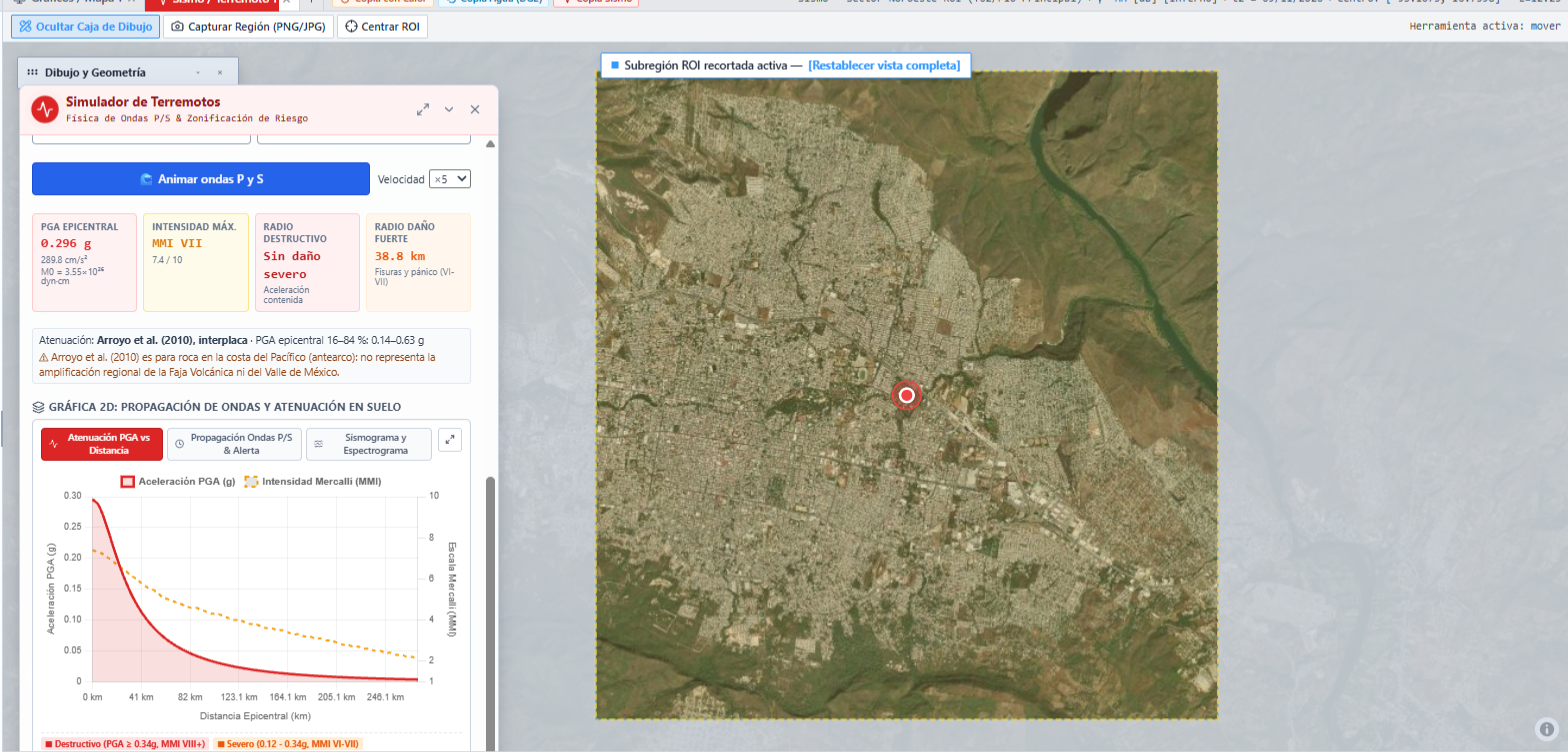
\includegraphics[width=0.84\textwidth]{fig/IMG_sismo_atenuacion_gmpe.png}
  \caption{Seismic simulator panel and modal displaying the 2D attenuation curve $\mathrm{PGA}(D)$ versus
  epicentral distance, the logarithmic uncertainty band ($16\text{--}84\,\text{\char37}$), scalar seismic moment
  $M_0$, and automatic validity-domain warnings for the selected GMPE model.}
  \label{fig:sismo-atenuacion-gmpe}
\end{figure}

\section{Elastodynamics, Travel Times, and 2D Wavefronts}
\label{sec:sismo-ondas}

\subsection{Body-Wave Velocities (P and S) and Early Warning Window}
\label{sec:sismo-tiempos}

In a continuous, homogeneous, isotropic, linear-elastic medium of density $\rho$ and Lam\'e constants $\lambda$
and $\mu$, the Navier--Cauchy equation of motion admits two decoupled body-wave solutions propagating from the
hypocenter at constant velocities:
\begin{equation}
  V_p = \sqrt{\frac{\lambda + 2\mu}{\rho}} \approx 6.0\,\unit{km/s},
  \qquad
  V_s = \sqrt{\frac{\mu}{\rho}} \approx 3.5\,\unit{km/s}.
  \label{eq:velocidades-ps}
\end{equation}
The primary $P$ wave (compressional or longitudinal) always travels faster than the secondary $S$ wave (shear or
transverse, responsible together with surface waves for the largest horizontal ground accelerations). For a
station located at hypocentral distance $R = \sqrt{D^2 + h^2}$, arrival times measured from earthquake origin
time ($t=0$) are:
\begin{equation}
  t_p = \frac{R}{V_p} = \frac{\sqrt{D^2 + h^2}}{V_p},
  \qquad
  t_s = \frac{R}{V_s} = \frac{\sqrt{D^2 + h^2}}{V_s}.
  \label{eq:tiempos-arribo}
\end{equation}
The lag between both arrivals defines the $P\text{--}S$ time window:
\begin{equation}
  \Delta t_{ps}(D,h) = t_s - t_p = R\left(\frac{1}{V_s} - \frac{1}{V_p}\right)
  \approx 0.1190\,\sqrt{D^2 + h^2}\quad[\unit{s}].
  \label{eq:ventana-ps}
\end{equation}
Additionally, the module reports the lead time from origin accounting for a fixed instrumental detection and
telemetry delay $t_{\mathrm{proc}} = 3.0\,\unit{s}$ (\texttt{sasmexAlertTimeSec}):
\begin{equation}
  T_{\mathrm{alert}}(D,h) = \max\!\left(0,\ t_s - t_{\mathrm{proc}}\right)
  = \max\!\left(0,\ \frac{\sqrt{D^2 + h^2}}{V_s} - 3.0\,\unit{s}\right).
  \label{eq:tiempo-sasmex}
\end{equation}

\begin{intuicion}
Equation~\eqref{eq:ventana-ps} is the physical clock that makes seismic early warning systems possible: every
additional $8.4\,\unit{km}$ of hypocentral distance gains roughly $1\,\unit{s}$ of separation between the $P$
wave (detected first by near-coast sensors) and the destructive $S$ wave. Because radio and fiber-optic signals
travel at nearly $300\,000\,\unit{km/s}$ compared to $3.5\,\unit{km/s}$ for the $S$ wave, an inland city far from
the focus receives the alert tens of seconds before the shear wave train arrives.
\end{intuicion}

\subsection{2D Surface Wavefront Kinematics}
\label{sec:sismo-frentes-2d}

When the user activates \textbf{Animate P and S waves}, the MapLibre canvas draws the intersection of the two
three-dimensional spherical wavefronts with Earth's surface as a function of elapsed time $t$ since rupture
initiation. Because the focus is buried at depth $h$, a spherical wavefront of radius $V\cdot t$ does not reach
the surface until the epicentral emergence instant $t_{\mathrm{em}} = h/V$. For any $t \ge 0$, the apparent
epicentral radius $r_w(t)$ of the wavefront on the map (\texttt{wavefrontSurfaceRadiusKm}) is:
\begin{equation}
  r_w(t;\ V, h) =
  \begin{cases}
    \sqrt{(V\,t)^2 - h^2}, & \text{if } V\,t > h,\\[4pt]
    0, & \text{if } V\,t \le h,
  \end{cases}
  \qquad
  V \in \{V_p,\ V_s\}.
  \label{eq:radio-frente-superficie}
\end{equation}
Differentiating with respect to time for $V t > h$, the apparent horizontal expansion speed of the ring on the map
is $\dd r_w/\dd t = V^2 t / \sqrt{(Vt)^2 - h^2} > V$: near the epicenter the wavefront appears to expand rapidly
as it emerges almost vertically from depth $h$, and asymptotically approaches the true wave speed $V$ at large
distances ($D \gg h$).

\begin{figure}[htbp]
  \centering
  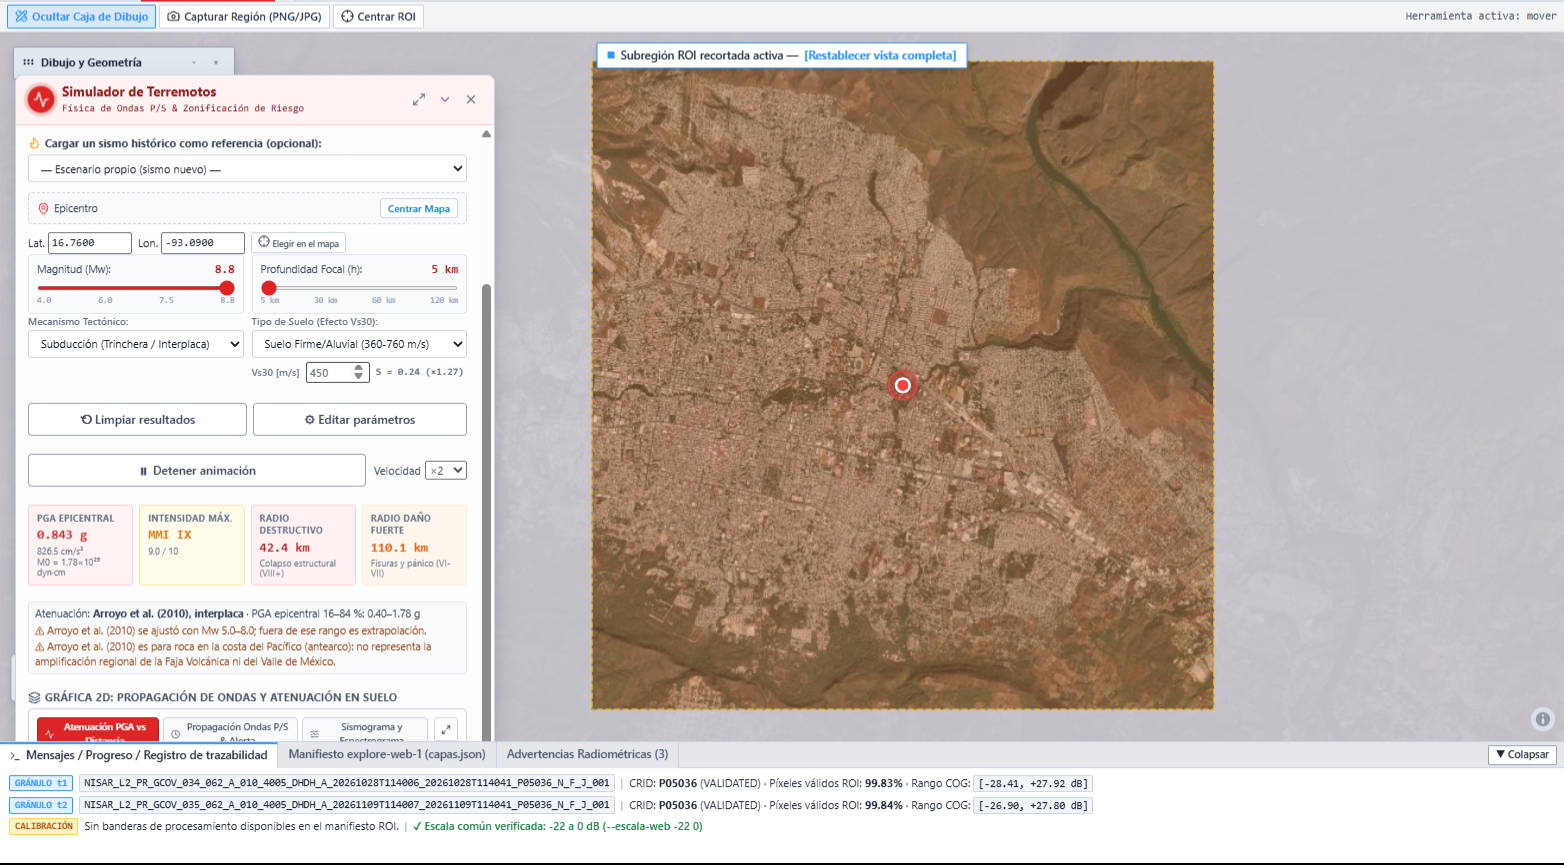
\includegraphics[width=0.84\textwidth]{fig/IMG_sismo_propagacion_2d_mapa.png}
  \caption{2D visual simulation on MapLibre GL showing the four geodesic isoseismal rings ($\mathrm{MMI}$),
  real-time concentric propagation of the $P$ (blue, $V_p=6.0\,\unit{km/s}$) and $S$ (red,
  $V_s=3.5\,\unit{km/s}$) wavefronts governed by Equation~\eqref{eq:radio-frente-superficie}, the interactive
  epicenter, and the receiving station selected on the map.}
  \label{fig:sismo-propagacion-2d}
\end{figure}

\section{Synthesis and Digital Signal Processing of the Seismic Waveform}
\label{sec:sismo-dsp}

\subsection{Formulation of the 50\,Hz Synthetic Accelerogram \texorpdfstring{$a(t)$}{a(t)}}
\label{sec:sismo-acelerograma}

For a station located at epicentral distance $D$ with geotechnical parameter $V_{s30,\mathrm{est}}$, the function
\texttt{synthesizeSeismogram} first evaluates local peak ground acceleration
$A_{\max} = \mathrm{PGA}_g(D, M_w, h, V_{s30,\mathrm{est}})$ and samples the time series at discrete instants
$t_n = n / f_m$ ($n=0,1,\ldots,N_{\mathrm{tot}}-1$) at a fixed sampling rate $f_m = 50\,\unit{Hz}$
($\Delta t = 0.02\,\unit{s}$, Nyquist frequency $f_{\mathrm{Nyq}} = 25\,\unit{Hz}$, well above all components of
the $P$ packet). The total signal is the superposition of three regimes:
\begin{equation}
  a(t) = a_{\mathrm{bg}}(t) + a_P(t) + a_S(t)\quad[g].
  \label{eq:acelerograma-total}
\end{equation}

\begin{enumerate}
  \item \textbf{Background microtremor ($a_{\mathrm{bg}}$):} low-amplitude deterministic background vibration
        present throughout the record:
        \begin{equation}
          a_{\mathrm{bg}}(t) = A_{\max}\bigl[0.0012\sin(11.2\,t + 0.3) + 0.0006\cos(23.7\,t)\bigr].
          \label{eq:sismo-fondo}
        \end{equation}
  \item \textbf{Primary $P$-wave packet ($t_p \le t < t_s$):} with local time $\tau_p = t - t_p$ and carrier
        frequency $f_P = 4.5\,\unit{Hz}$, modeled as an amplitude-modulated packet with exponential decay:
        \begin{equation}
          a_P(t) = 0.22\,A_{\max}\,\sin(2\pi f_P \tau_p)\,\cos(0.3\pi f_P \tau_p)\,
                   \exp\!\left(-\frac{\tau_p}{3.2\,\unit{s}}\right)\,
                   \bigl[\mathcal{H}(t - t_p) - \mathcal{H}(t - t_s)\bigr],
          \label{eq:sismo-onda-p}
        \end{equation}
        where $\mathcal{H}$ is the Heaviside step function. By the trigonometric identity
        $\sin\alpha\cos\beta = \tfrac12[\sin(\alpha+\beta)+\sin(\alpha-\beta)]$, the modulating product splits
        the spectral energy of the $P$ wave into two sidebands located at
        $0.85\,f_P = 3.825\,\unit{Hz}$ and $1.15\,f_P = 5.175\,\unit{Hz}$.
  \item \textbf{Secondary $S$-wave packet and surface coda ($t \ge t_s$):} with local time $\tau_s = t - t_s$,
        soil-dependent fundamental frequency $f_S(V_{s30,\mathrm{est}})$, and a phase-shifted first harmonic:
        \begin{equation}
          a_S(t) = A_{\max}\,E_S(\tau_s)\,\Bigl[
            0.82\sin(2\pi f_S \tau_s) + 0.18\sin(4\pi f_S \tau_s + 0.6)
          \Bigr]\,\mathcal{H}(t - t_s),
          \label{eq:sismo-onda-s}
        \end{equation}
        governed by the linear-attack and exponential-coda envelope $E_S(\tau_s)$:
        \begin{equation}
          E_S(\tau_s) =
          \begin{cases}
            \dfrac{\tau_s}{1.8\,\unit{s}}, & \text{if } 0 \le \tau_s \le 1.8\,\unit{s},\\[8pt]
            \exp\!\left(-\dfrac{\tau_s - 1.8\,\unit{s}}{\tau_{\mathrm{coda}}(V_{s30,\mathrm{est}})}\right), &
              \text{if } \tau_s > 1.8\,\unit{s}.
          \end{cases}
          \label{eq:envolvente-s}
        \end{equation}
\end{enumerate}
As shown in Table~\ref{tab:comparacion-vs30}, in a soft lacustrine basin ($V_{s30} < 180\,\unit{m/s}$, such as
the clays of the former Lake Texcoco in Mexico City), the fundamental frequency drops to
$f_S = 0.52\,\unit{Hz}$ (period $T_0 \approx 1.92\,\unit{s}$) and the decay time constant lengthens to
$\tau_{\mathrm{coda}} = 28\,\unit{s}$, reproducing prolonged quasi-harmonic site resonance.

\subsection{Arias Intensity (\texorpdfstring{$I_A$}{IA}) and Significant Duration \texorpdfstring{$D_{5\text{--}95}$}{D5-95}}
\label{sec:sismo-arias}

Peak amplitude $\mathrm{PGA}$ measures a single instant of the seismogram, whereas cumulative destructive
potential also depends on how long the ground keeps shaking. \textbf{Arias Intensity} $I_A$ (Arias, 1970) is
defined as the total energy per unit weight dissipated by a bank of undamped linear oscillators over the entire
duration $T_{\mathrm{tot}}$ of ground motion:
\begin{equation}
  I_A = \frac{\pi}{2\,g_0}\int_0^{T_{\mathrm{tot}}} a^2(t)\,\dd t\quad[\unit{m/s}].
  \label{eq:intensidad-arias}
\end{equation}
From the time evolution of cumulative energy, the normalized Husid function $H(t)\in[0,1]$ is defined as:
\begin{equation}
  H(t) = \frac{\displaystyle\int_0^t a^2(\tau)\,\dd\tau}{\displaystyle\int_0^{T_{\mathrm{tot}}} a^2(\tau)\,\dd\tau}
  \;\approx\;
  \frac{\displaystyle\sum_{n=0}^{k} a_n^2}{\displaystyle\sum_{n=0}^{N_{\mathrm{tot}}-1} a_n^2},
  \qquad t = \frac{k}{f_m}.
  \label{eq:husid}
\end{equation}
Following the criterion of Trifunac and Brady (1975), the \textbf{significant duration} $D_{5\text{--}95}$
(\texttt{significantDurationSec} in \src{web/src/utils/signal.ts}) is the time interval over which the central
$90\,\text{\%}$ of Arias energy is released, i.e., between instants $t_{5\%}$ and $t_{95\%}$ where $H(t)$ reaches
$0.05$ and $0.95$:
\begin{equation}
  D_{5\text{--}95} = t_{95\%} - t_{5\%},
  \qquad
  H(t_{5\%}) = 0.05,\quad H(t_{95\%}) = 0.95.
  \label{eq:duracion-d5-95}
\end{equation}
Note that in~\eqref{eq:husid} the physical constant $\pi/(2g_0)$ and time step $\Delta t = 1/f_m$ cancel out
exactly between numerator and denominator, making $D_{5\text{--}95}$ invariant to the engineering unit scale of
the accelerogram ($g$, $\unit{m/s^2}$, or $\unit{gal}$).

\subsection{Fast Fourier Transform (FFT) and Time-Frequency Spectrogram (STFT)}
\label{sec:sismo-fft-stft}

To analyze the frequency distribution of either the synthetic waveform or a user-loaded instrumental record
(\src{web/src/utils/accelerogram.ts}), \src{web/src/utils/signal.ts} implements an in-place radix-2
Cooley--Tukey Fast Fourier Transform (FFT) with bit-reversal permutation.

\subsubsection*{1. Global Spectrum and Dominant Frequency}
Given a zero-mean series $\tilde a_n = a_n - \bar{a}$ of length $N_s$, to estimate the dominant frequency
(\texttt{dominantFrequencyHz}) with high spectral precision, the signal is multiplied by a smooth Hann window
\begin{equation}
  w(n) = \frac{1}{2} - \frac{1}{2}\cos\!\left(\frac{2\pi n}{N_s - 1}\right),
  \qquad n = 0,1,\ldots,N_s - 1,
  \label{eq:ventana-hann}
\end{equation}
and zero-padded to a power-of-two length $N_{\mathrm{FFT}} = 2^{\lceil\log_2\max(8N_s, 1024)\rceil}$, which
interpolates the spectrum with fine frequency spacing $\Delta f = f_m / N_{\mathrm{FFT}}$. The Discrete Fourier
Transform (DFT) and dominant frequency $f_{\mathrm{dom}}$ are computed as:
\begin{equation}
  \widehat{A}(k) = \sum_{n=0}^{N_{\mathrm{FFT}}-1} \tilde a_n\,w(n)\,e^{-2\pi\mathrm{i}kn/N_{\mathrm{FFT}}},
  \qquad
  k^\ast = \arg\max_{1\le k \le N_{\mathrm{FFT}}/2} \bigl|\widehat{A}(k)\bigr|^2,
  \qquad
  f_{\mathrm{dom}} = \frac{k^\ast\,f_m}{N_{\mathrm{FFT}}}\quad[\unit{Hz}].
  \label{eq:fft-dominante}
\end{equation}

\subsubsection*{2. Short-Time Fourier Transform (STFT) Spectrogram}
Because a seismogram is a strongly non-stationary signal (first the higher-frequency $P$ wave arrives in
$3.8\text{--}5.2\,\unit{Hz}$, and seconds later the $S$ wave bursts in at $0.52\text{--}2.20\,\unit{Hz}$), a
single global FFT cannot show \emph{when} each frequency acts. The function \texttt{computeSpectrogram} evaluates
the Short-Time Fourier Transform (STFT) by sliding a Hann window $w(n)$ of length
$N_w = 2^{\lceil\log_2(4\,f_m)\rceil}$ samples (at $50\,\unit{Hz}$, $N_w = 256$ samples $= 5.12\,\unit{s}$, with
frequency resolution $\Delta f = 50/256 \approx 0.195\,\unit{Hz}$) using a hop size of
$H = N_w / 8 = 32$ samples ($0.64\,\unit{s}$, $87.5\,\text{\%}$ overlap):
\begin{equation}
  X(m,k) = \sum_{n=0}^{N_w - 1} a(mH + n)\,w(n)\,e^{-2\pi\mathrm{i}kn/N_w},
  \qquad
  k \in \left\{0,1,\ldots,\frac{N_w}{2}\right\},
  \label{eq:stft-definicion}
\end{equation}
where frame index $m$ is centered at physical instant $t_m = (mH + N_w/2)/f_m$ and spectral bin $k$ corresponds
to frequency $f_k = k\,f_m/N_w$. The power spectral density matrix in decibels is:
\begin{equation}
  P_{\mathrm{dB}}(m,k) = 10\log_{10}\!\Bigl(\bigl|X(m,k)\bigr|^2 + 10^{-20}\Bigr)\quad[\unit{dB}],
  \label{eq:stft-db}
\end{equation}
which is rendered on the canvas of \src{web/src/components/SeismogramSpectrogram.tsx} using the scientific
\emph{Inferno} colormap across a $60\,\unit{dB}$ dynamic range below the global maximum
$\max_{m,k} P_{\mathrm{dB}}(m,k)$, vertically aligning the time axis of $a(t)$ with that of the spectrogram and
marking the $t_p$, $t_s$ arrival lines and $\Delta t_{ps}$ window on both views.

\begin{ejemplo}[Quantitative contrast in a Michoac\'an 1985-type scenario at $D=350\,\unit{km}$]
Placing an interplate earthquake of $M_w = 8.1$ at focal depth $h = 15\,\unit{km}$ (hypocentral distance
$R = \sqrt{350^2 + 15^2} = 350.32\,\unit{km}$), arrival times at the station are
$t_p = 350.32/6.0 = 58.39\,\unit{s}$ and $t_s = 350.32/3.5 = 100.09\,\unit{s}$, yielding a window
$\Delta t_{ps} = 41.70\,\unit{s}$. Varying only the receiving station parameter $V_{s30}$ in the simulator:
\begin{itemize}
  \item \textbf{Station on firm rock ($V_{s30} = 760\,\unit{m/s}$):} the spectrogram concentrates $S$-wave
        energy at $f_{\mathrm{dom}} = 2.20\,\unit{Hz}$ and shaking decays rapidly with significant duration
        $D_{5\text{--}95} = 13.3\,\unit{s}$.
  \item \textbf{Station on lacustrine clay ($V_{s30} = 100\,\unit{m/s}$):} the site factor amplifies peak
        acceleration by $2.49\times$, spectrogram energy migrates to the low-frequency band
        $f_{\mathrm{dom}} = 0.52\,\unit{Hz}$, and Arias significant duration nearly triples to
        $D_{5\text{--}95} = 33.4\,\unit{s}$.
\end{itemize}
\end{ejemplo}

\begin{figure}[htbp]
  \centering
  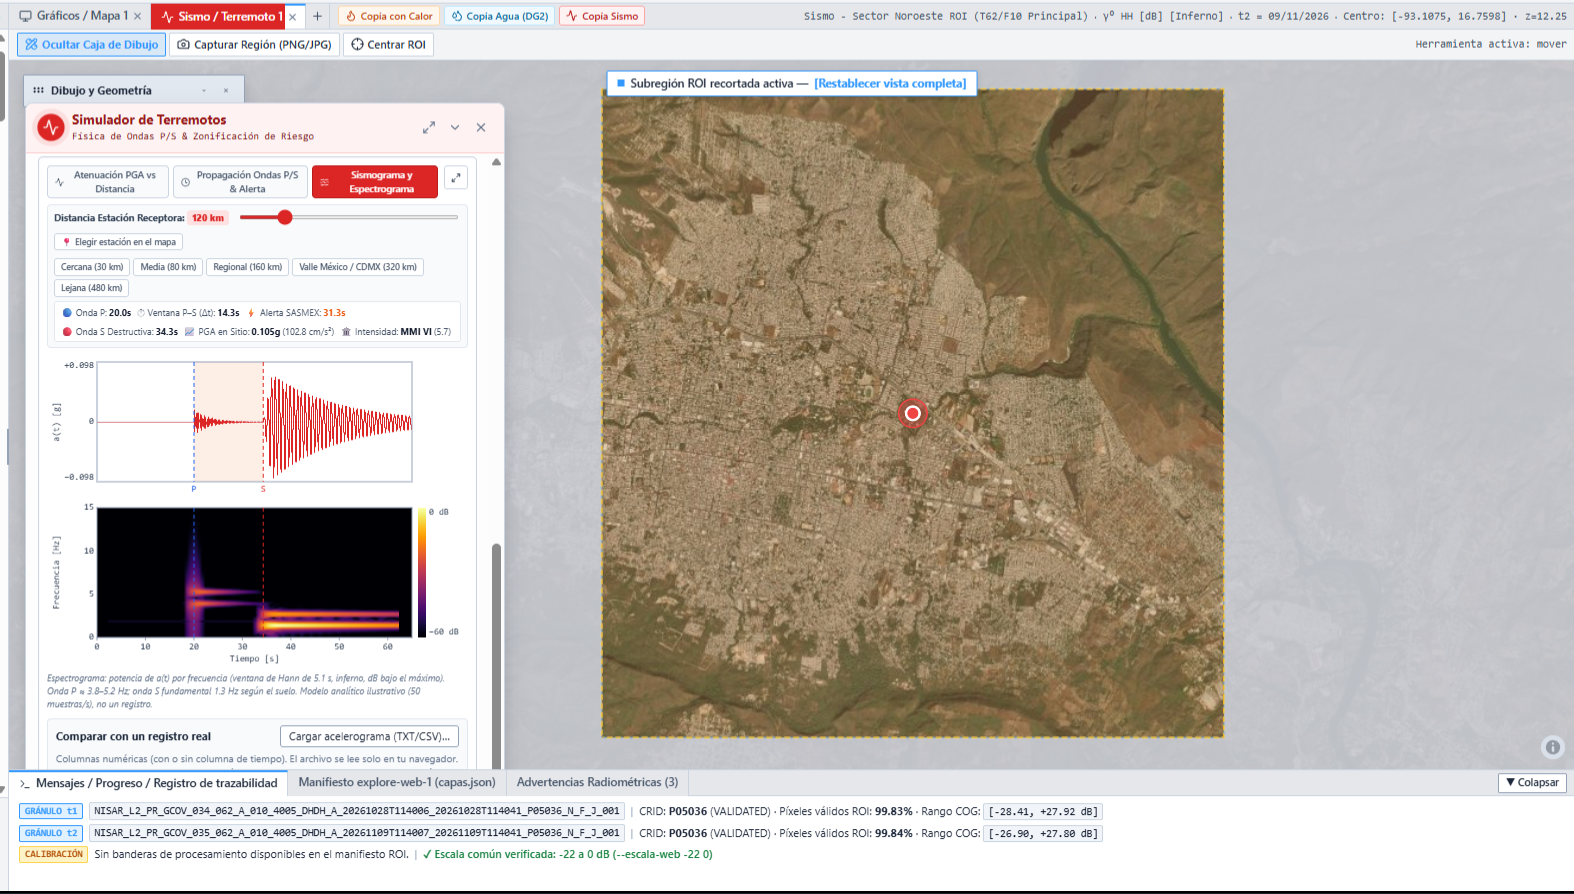
\includegraphics[width=0.84\textwidth]{fig/IMG_sismo_sismograma_espectrograma.png}
  \caption{Coupled view of the synthetic accelerogram time series $a(t)$ sampled at $50\,\unit{Hz}$ (top) and its
  Hann-windowed STFT time-frequency spectrogram on a $60\,\unit{dB}$ \emph{Inferno} scale (bottom). Both $P$-wave
  sidebands ($3.8$ and $5.2\,\unit{Hz}$ between $t_p$ and $t_s$) and the low-frequency energy concentration
  following $S$-wave arrival are clearly resolved alongside the $f_{\mathrm{dom}}$ and $D_{5\text{--}95}$
  metrics.}
  \label{fig:sismo-sismograma-stft}
\end{figure}

\clearpage
\part{Software Architecture, APIs, and Deployment}
\label{part:arquitectura-apis-docker}

This part documents the software engineering, inter-subsystem data contracts, geospatial persistence, and
containerization scheme that sustain the end-to-end operation of TerraPulse AI. Its design obeys a central
architectural premise established in \src{AGENTS.md}: the scientific radar and geophysical processing core
(\src{pipeline/}) is \textbf{pure Python and completely independent of the web server}, whereas the application
layer (\src{backend/} and \src{web/}) acts as an orchestrator, spatial store, and interactive viewer that
preserves end-to-end traceability intact from the original HDF5 or HGT file down to every pixel and chart
rendered in the browser.

\section{Overall System Architecture and Contract-Based Decoupling}
\label{sec:arq-general}

The platform is structured into four decoupled layers that communicate through strictly versioned data contracts
(Contracts C1 through C5, plus the on-demand ROI job and solar simulation contracts):

\begin{enumerate}
  \item \textbf{Scientific Processing Layer (\src{pipeline/}, Python 3.11):}
        modules independent of any HTTP framework (\src{catalog.py}, \src{compat.py}, \src{nisar\_h5.py},
        \src{download.py}, \src{etapa1.py}, \src{web\_export.py}, \src{graficas\_datos.py}, \src{preprocess.py},
        \src{change.py}, \src{roi\_explore.py}, \src{elevation/nasadem.py}, and \src{solar/}). It reads remote
        ASF \texttt{.h5} granules over HTTPS via $8\,\unit{MiB}$ \emph{HTTP Range Requests} (\texttt{fsspec} and
        \texttt{h5py}) as well as \texttt{NASADEM\_HGT} version \texttt{001} tiles, producing 32-bit floating-point
        GeoTIFFs, Cloud-Optimized GeoTIFFs (COGs), reprojected PNG overlays, and JSON manifests stamped with the
        exact Git commit hash (\texttt{version\_codigo}).
  \item \textbf{Service and REST API Layer (\src{backend/}, Python / Django 5.2 + GeoDjango + DRF 3.18):}
        although the initial challenge proposal considered FastAPI as a lightweight Python server, the final
        implementation adopted \textbf{Django + GeoDjango + Django REST Framework (DRF)} because it provides a
        native spatial ORM over PostGIS (\texttt{PolygonField} with SRID 4326, \texttt{intersects} geometric
        queries), a transactional migration engine (\src{scenes/migrations/}), reproducible management commands
        (\texttt{manage.py load\_explore}), and an inspection audit panel (\texttt{/admin/}) without boilerplate,
        while preserving the exact same logical separation of JSON REST services as a FastAPI layout.
  \item \textbf{Spatial Persistence and Transactional Cache Layer (PostgreSQL 16 + PostGIS 3.4 + filesystem):}
        vector geometries (\texttt{ROI}, scene \texttt{footprint} polygons), catalog-verified orbital metadata,
        and numerical inspection series (\texttt{jsonb}) reside in PostGIS inside a Docker container backed by a
        persistent volume (\texttt{pgdata}). Heavy raster products ($32\text{-bit}$ GeoTIFF/COG files and visual
        PNGs) are stored in immutable hash-indexed disk hierarchies (\path{data/explore/}, \path{data/roi-runs/},
        \path{data/graficas-roi/}, \path{data/solar-runs/}, and \path{data/nasadem-cache/}).
  \item \textbf{Presentation and Interaction Layer (\src{web/}, React 19 + TypeScript + Vite + MapLibre GL + Chart.js):}
        a single-page application (SPA) that consumes REST APIs through a same-origin proxy
        (\texttt{/api} $\to$ \texttt{http://localhost:8000}), overlays georeferenced rasters onto MapLibre GL,
        renders statistical distributions with a $p_{0.2}\text{--}p_{99.8}$ CDF window in Chart.js, and executes
        the solar LUT inversion, 3D topographic viewer, and seismic simulator modules directly on the client.
\end{enumerate}

\begin{figure}[htbp]
\centering
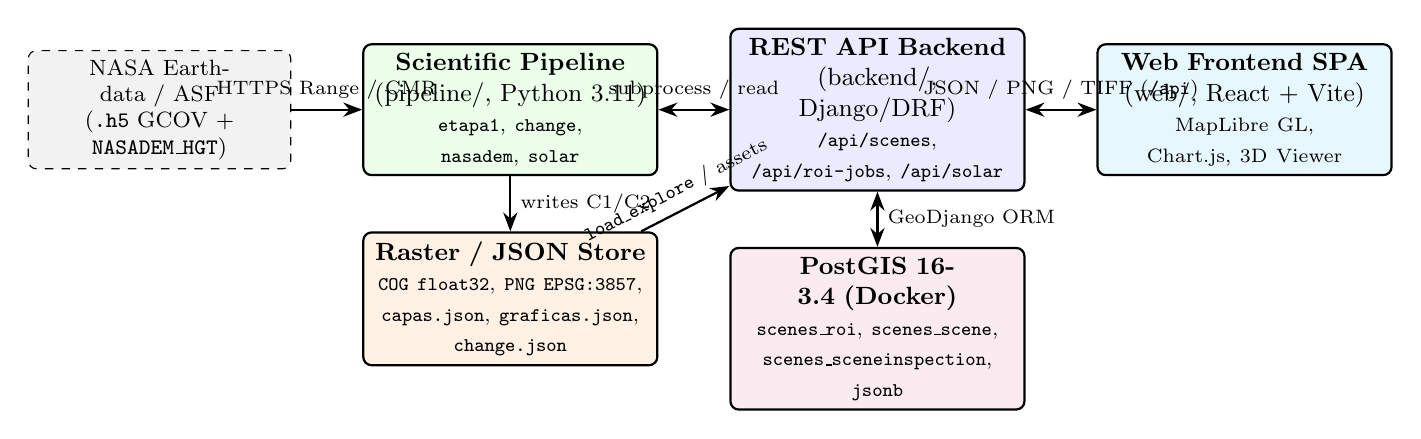
\begin{tikzpicture}[
  node distance=7mm and 9mm,
  capa/.style={draw,rounded corners=3pt,thick,align=center,font=\small,minimum height=1.35cm,text width=3.5cm},
  ext/.style={draw,dashed,rounded corners=3pt,fill=gray!10,align=center,font=\footnotesize,minimum height=1.1cm,text width=3.1cm},
  fl/.style={-{Stealth[length=2.4mm]},thick},
  flb/.style={{Stealth[length=2.4mm]}-{Stealth[length=2.4mm]},thick}
]
  \node[ext] (asf) {NASA Earthdata / ASF\\(\texttt{.h5} GCOV + \texttt{NASADEM\_HGT})};
  \node[capa,fill=green!8,right=of asf] (pipe) {\textbf{Scientific Pipeline}\\(\src{pipeline/}, Python 3.11)\\{\scriptsize \texttt{etapa1}, \texttt{change}, \texttt{nasadem}, \texttt{solar}}};
  \node[capa,fill=blue!8,right=of pipe] (api) {\textbf{REST API Backend}\\(\src{backend/}, Django/DRF)\\{\scriptsize \texttt{/api/scenes}, \texttt{/api/roi-jobs}, \texttt{/api/solar}}};
  \node[capa,fill=purple!8,below=of api] (db) {\textbf{PostGIS 16-3.4 (Docker)}\\{\scriptsize \texttt{scenes\_roi}, \texttt{scenes\_scene},}\\{\scriptsize \texttt{scenes\_sceneinspection}, \texttt{jsonb}}};
  \node[capa,fill=orange!10,below=of pipe] (fs) {\textbf{Raster / JSON Store}\\{\scriptsize \texttt{COG float32}, \texttt{PNG EPSG:3857},}\\{\scriptsize \texttt{capas.json}, \texttt{graficas.json}, \texttt{change.json}}};
  \node[capa,fill=cyan!10,right=of api] (web) {\textbf{Web Frontend SPA}\\(\src{web/}, React + Vite)\\{\scriptsize MapLibre GL, Chart.js, 3D Viewer}};

  \draw[fl] (asf) -- node[above,font=\scriptsize]{HTTPS Range / CMR} (pipe);
  \draw[fl] (pipe) -- node[right,font=\scriptsize]{writes C1/C2} (fs);
  \draw[flb] (api) -- node[above,font=\scriptsize]{subprocess / read} (pipe);
  \draw[fl] (fs) -- node[above,sloped,font=\scriptsize]{\texttt{load\_explore} / assets} (api);
  \draw[flb] (api) -- node[right,font=\scriptsize]{GeoDjango ORM} (db);
  \draw[flb] (api) -- node[above,font=\scriptsize]{JSON / PNG / TIFF (\texttt{/api})} (web);
\end{tikzpicture}
\caption{Four-layer decoupled architecture of TerraPulse AI. The scientific pipeline (\src{pipeline/}) imports no
web server modules; communication occurs through on-disk contracts and spatial tables in PostGIS.}
\label{fig:arquitectura-4-capas}
\end{figure}

\begin{figure}[htbp]
  \centering
  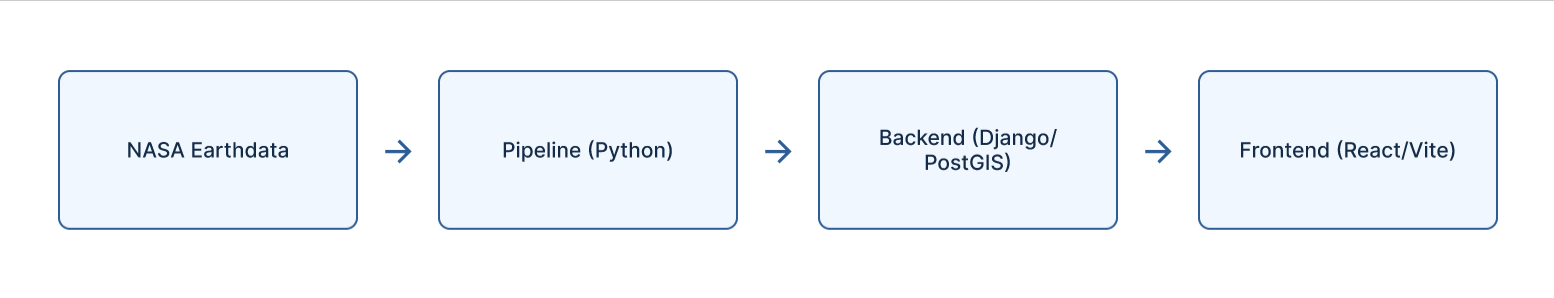
\includegraphics[width=0.86\textwidth]{fig/IMG_arquitectura_general_sistema.png}
  \caption{Comprehensive software architecture diagram of TerraPulse AI, illustrating the data flow from NASA
  Earthdata repositories (ASF Vertex and LP DAAC) to the Python backend (Django/DRF), the PostgreSQL 16 +
  PostGIS 3.4 Docker container, and the interactive React/Vite frontend modules.}
  \label{fig:img-arquitectura-general}
\end{figure}

\subsection{Summary of Internal Repository Contracts}

Table~\ref{tab:contratos-internos} synthesizes the formal contracts that isolate each stage of the data pipeline.

\begin{table}[htbp]
\centering
\small
\begin{tabular}{lp{3.4cm}p{3.6cm}p{5.8cm}}
\toprule
\textbf{Contract} & \textbf{Producer} & \textbf{Consumer} & \textbf{Key Artifacts and Guarantees} \\
\midrule
\textbf{C1 (Subset)} & \src{pipeline/download.py}, \src{sources/subset.py} & \src{pipeline/preprocess.py}, \src{pipeline/change.py} & \path{data/raw/<scene_id>/<capa>.tif} + \path{scene.json}. Identity verified against catalog and native UTM grid without resampling. \\
\textbf{Stage 1 Web} & \src{pipeline/etapa1.py}, \src{web\_export.py}, \src{graficas\_datos.py} & \texttt{load\_explore}, \src{roi\_explore.py}, MapLibre/Chart.js Frontend & \path{web/capas.json} (\texttt{explore-web-1}), \texttt{float32} COG in UTM, RGBA PNG in \texttt{EPSG:3857}, and \path{graficas.json} (\texttt{graficas-etapa1-1}). \\
\textbf{C2 (Change $\Delta$)} & \src{pipeline/change.py}, \src{roi\_explore.py} & \texttt{/api/roi-jobs} service, \src{ChangeControls.tsx} & \path{delta_<pol>_dB.tif}, \path{zscore_<pol>.tif}, \path{cambio_<pol>.tif}, \path{change.json}, and \path{web/capas.json} with $\sigma_{\mathrm{MAD}}$ and $\tau_{\mathrm{dB}} < 3\sigma_{\mathrm{MAD}}$ alert. \\
\textbf{C4 (REST API)} & \src{backend/scenes/}, \src{backend/solar/} & \src{web/src/api/client.ts}, React hooks & UTF-8 JSON responses, GeoJSON geometries in \texttt{EPSG:4326} (\texttt{[lon, lat]}), ISO~8601 UTC timestamps, and traceability fields (\texttt{code\_version}, \texttt{warnings}). \\
\textbf{C5 (Tiles)} & TiTiler server / \src{roi\_views.py} & MapLibre GL (\texttt{ImageSource} / \texttt{RasterSource}) & Numerical value queries from COG (\texttt{float32}) and visual overlay via PNG in \texttt{EPSG:3857} or \texttt{EPSG:4326}. \\
\bottomrule
\end{tabular}
\caption{Data contracts across TerraPulse AI subsystems.}
\label{tab:contratos-internos}
\end{table}

\section{Stage 1 Web Export and Statistical Visualization in Chart.js}
\label{sec:arq-etapa1-chartjs}

Before a NISAR GCOV scene reaches the database or the browser, \src{pipeline/etapa1.py} executes the radiometric
and geometric inspection over the ROI, either from a local \texttt{.h5} file or directly in remote HTTPS streaming
mode using its \texttt{scene\_id}.

\subsection{Remote HTTPS Block Reading and Identity Verification}

When invoking \texttt{python -m pipeline.etapa1 <scene\_id> --escala-web -22 0}, the pipeline avoids downloading
the full GCOV granule ($\sim 7\,\unit{GB}$) by executing six deterministic steps:
\begin{enumerate}
  \item Locates \texttt{scene\_id} in the latest catalog (\path{data/catalog/catalog_*.json}) and extracts its
        signed ASF HTTPS URL together with its catalog maturity level (\texttt{dataMaturity}).
  \item Initializes an authenticated NASA Earthdata session (\texttt{earthdata\_https\_fs()}, prioritizing
        \texttt{EARTHDATA\_USERNAME}/\texttt{EARTHDATA\_PASSWORD} environment variables over \path{~/.netrc}).
  \item Opens the remote HDF5 container via \texttt{h5py} over an \texttt{fsspec} HTTPS file object with an
        $8\,\unit{MiB}$ block cache, transferring over the network only those internal HDF5 chunks that intersect
        the ROI bounding window and the incidence-angle geolocation cube.
  \item Executes \texttt{check\_identity}: verifies that internal HDF5 attributes (\texttt{granuleId},
        \texttt{CRID}, track, frame, and orbital pass direction) match the catalog record exactly; any mismatch
        aborts execution immediately.
  \item Computes the $\gz$ and $\sz = \gz \cdot F$ matrices in memory, applies the subswath validity mask and
        the $2\times 2$ inspection Multilook ($20\,\unit{m}$), and exports both scientific GeoTIFFs and the
        \path{web/} directory (\src{pipeline/web\_export.py}) along with the chart series (\path{graficas.json},
        \src{pipeline/graficas\_datos.py}).
  \item In remote mode, omits Figure~A ($1:50$ subsampled full-scene overview) by default because reading 1 out of
        every 50 pixels across the granule would touch nearly every HDF5 chunk in the $7\,\unit{GB}$ file.
\end{enumerate}

\subsection{COG (\texttt{EPSG:32615}) vs.\ PNG (\texttt{EPSG:3857}) Duality and the \texttt{capas.json} Manifest}

A foundational technical principle of the web layer is the strict separation between \textbf{measurement files}
and \textbf{visual rendering files}:
\begin{itemize}
  \item \textbf{Cloud-Optimized GeoTIFF (\path{web/<magnitud>_<capa>_ml2_dB.tif}):} stores exact decibel values
        in \texttt{float32} format ($\mathrm{NaN}$ for nodata pixels), in the product's native UTM projection
        (e.g., \texttt{EPSG:32615}), compressed with \texttt{DEFLATE} in $512\times 512$-pixel internal blocks
        and equipped with \textbf{nearest-neighbor} overviews (never averaging decibels). It serves as the sole
        source for point value queries and TiTiler interoperability.
  \item \textbf{Overlay Image (\path{web/<magnitud>_<capa>_ml2_dB.png}):} an 8-bit-per-channel RGBA image
        pre-reprojected to \textbf{Web Mercator (\texttt{EPSG:3857})}, rendered with a linear grayscale ramp
        between \texttt{vmin\_dB} and \texttt{vmax\_dB} and alpha channel $\alpha = 0$ where no valid data exists.
\end{itemize}

\begin{intuicion}
\textbf{Why must the PNG for MapLibre be reprojected to \texttt{EPSG:3857} while the COG remains in UTM?}
When MapLibre GL renders an \texttt{image}-type layer from its four geographic corner coordinates
(\texttt{esquinas\_lonlat}), it stretches the image pixel rectangle directly onto the flat Web Mercator canvas
(\texttt{EPSG:3857}). A UTM grid (\texttt{EPSG:32615}) exhibits slight meridian convergence relative to true
geographic north; if a UTM PNG were passed directly to MapLibre, pixels would appear slightly rotated and shifted
relative to basemap rivers and roads. By reprojecting the PNG to \texttt{EPSG:3857} in
\src{pipeline/web\_export.py} and computing its exact four corners in \texttt{EPSG:4326} (in the order required
by MapLibre: top-left, top-right, bottom-right, bottom-left), every pixel lands on its exact cartographic
position without requiring a tile server for immediate visual inspection.
\end{intuicion}

Below is the real structure of the \path{web/capas.json} manifest (version \texttt{explore-web-1}) generated for
scene $t_1$ of the Chiapas working pair:

\begingroup\scriptsize
\begin{verbatim}
{
  "version": "explore-web-1",
  "tipo": "inspeccion_una_fecha",
  "creado_utc": "2026-11-15T07:46:16Z",
  "version_codigo": "863fa3f",
  "escena": {
    "granuleId": "NISAR_L2_PR_GCOV_023_062_A_010_4005_DHDH_A_20260618T114010_20260618T114044_P05023_N_F_J_001",
    "producto": "GCOV",
    "fecha_inicio": "2026-06-18T11:40:10Z",
    "trayectoria": 62,
    "marco": 10,
    "direccion": "ASCENDING",
    "crid": "P05023",
    "madurez_catalogo": "PROVISIONAL",
    "frecuencia": "A",
    "polarizaciones": ["HH", "HV"]
  },
  "roi_wkt_4326": "POLYGON((-93.3919 16.6539,-92.8757 16.6539,-92.8757 16.8964,-93.3919 16.8964,-93.3919 16.6539))",
  "procedencia": {
    "modo": "remoto",
    "catalogo": "data/catalog/catalog_20261112T041822Z.json",
    "identidad_verificada_contra_catalogo": true
  },
  "capas": [
    {
      "id": "gamma0_HHHH_ml2_dB",
      "capa": "HHHH",
      "magnitud": "gamma0",
      "simbolo": "gamma0",
      "multilook": 2,
      "pixel_m": 20,
      "unidades": "dB",
      "cog": "data/explore/NISAR_L2_PR_GCOV_.../web/gamma0_HHHH_ml2_dB.tif",
      "png": "data/explore/NISAR_L2_PR_GCOV_.../web/gamma0_HHHH_ml2_dB.png",
      "crs_cog": "EPSG:32615",
      "crs_png": "EPSG:3857",
      "forma_cog": [1343, 2752],
      "forma_png": [1352, 2750],
      "esquinas_lonlat": [
        [-93.3924, 16.8968],
        [-92.8757, 16.8968],
        [-92.8757, 16.6536],
        [-93.3924, 16.6536]
      ],
      "escala": {
        "vmin_dB": -22.0,
        "vmax_dB": 0.0,
        "colormap": "gray",
        "metodo": "fija (--escala-web)"
      },
      "rango_datos_dB": [-34.58, 14.82],
      "pct_pixeles_validos": 99.574
    }
  ],
  "graficas": "data/explore/NISAR_L2_PR_GCOV_.../graficas.json",
  "metadatos": "data/explore/NISAR_L2_PR_GCOV_.../metadatos.json",
  "advertencias": [
    "Single date: intended for visual inspection, not for a change map.",
    "PNG layers are for display only; never compute differences on them.",
    "To compare two dates in the swipe slider, use the same --escala-web on both."
  ]
}
\end{verbatim}
\endgroup

\subsection{The \texttt{graficas.json} Contract and Scientific Chart.js Rendering (\src{Etapa1ChartsPanel.tsx})}

So that the frontend does not rely on static images when displaying radiometric distributions,
\src{pipeline/graficas\_datos.py} serializes into \path{graficas.json} (format \texttt{graficas-etapa1-1}) the
exact same numerical vectors used to plot scientific Figures C, D, and E:
\begin{enumerate}
  \item \texttt{histograma\_gamma0\_dB}: exact integer pixel counts per bin of width $\Delta b = 0.1\,\unit{dB}$
        across $[-60, +30]\,\unit{dB}$ at native resolution ($10\,\unit{m}$), per polarization
        (\texttt{HHHH}, \texttt{HVHV}). Empty leading and trailing bins are trimmed while preserving the exact
        conservation invariant:
        \begin{equation}
          \sum_{k=0}^{K-1} c_k = N_{\text{in-range}}, \qquad
          N_{\text{in-range}} + N_{\text{out-of-range}} = N_{\text{valid}}.
          \label{eq:invariante-histograma-etapa1}
        \end{equation}
        In real Chiapas scene $t_1$ (2026-06-18), the \texttt{HHHH} series contains $646$ active bins starting at
        $-34.6\,\unit{dB}$ plus $936$ pixels with $\gz > 30\,\unit{dB}$, summing to the exact $14\,694\,370$ valid
        pixels of the C1 subset ($8.3\,\unit{KB}$ in JSON). It also includes precomputed summary statistics:
        mean of dB values (\texttt{media\_dB}), median (\texttt{mediana\_dB}), decibel conversion of the linear
        mean ($\texttt{dB\_de\_la\_media} = 10\log_{10}\bar{\gz}$), standard deviation, and percentiles $p_5$ and
        $p_{95}$.
  \item \texttt{mascara\_roi}: percentage breakdown of the four \texttt{mask} layer categories within the ROI
        bounding window (valid in subswath, invalid~$0$, outside subswath~$255$, and nodata fill) together with
        the exact percentage of valid pixels inside the ROI polygon (\texttt{pct\_validos\_en\_poligono}).
  \item \texttt{incidencia\_por\_altura}: curve of the mean incidence angle over the ROI evaluated across all $21$
        height layers of the radar geolocation grid ($h \in [-1000, +9000]\,\unit{m}$ above the WGS84 ellipsoid),
        highlighting the $500\,\unit{m}$ reference level.
\end{enumerate}

\begin{cuidado}
\warn{Why a categorical bar chart in Chart.js distorts a SAR histogram and how \src{Etapa1ChartsPanel.tsx}
resolves it.}
If every $0.1\,\unit{dB}$ bin is passed as a categorical label inside a $360\,\unit{px}$-wide side panel canvas,
the horizontal axis spans nearly $68\,\unit{dB}$ (from $-38$ to $+30\,\unit{dB}$) simply because a handful of
bright corner reflectors populate the right tail. Because $90\,\text{\%}$ of pixels ($p_5\text{--}p_{95}$) are
concentrated within just $\sim 11\,\unit{dB}$ ($16\,\text{\%}$ of total width) and each bin gets only
$\sim 0.48\,\unit{px}$, the charting engine rounds sub-pixel positions and collapses the bell shape.

To prevent this without altering a single number in \path{graficas.json},
\src{web/src/components/Etapa1ChartsPanel.tsx} enforces four scientific plotting rules identical to those in
\src{pipeline/etapa1\_figuras.py}:
\begin{enumerate}
  \item \textbf{Cumulative Distribution Function windowing (CDF $p_{0.2}\text{--}p_{99.8}$):} sets the $X$-axis
        limits to the $0.002$ and $0.998$ quantiles of the distribution (e.g., in Chiapas $t_2$:
        $[-18.7, +7.5]\,\unit{dB}$ for HH and $[-24.0, -1.7]\,\unit{dB}$ for HV) and explicitly reports in the
        caption the exact percentage of pixels lying outside the display window ($\approx 0.46\,\text{\%}$).
  \item \textbf{Continuous linear $X$ axis with step trace (\texttt{stepped: 'middle'}):} each bin $k$ is placed
        at its exact physical center $x_k = b_0 + (k + 0.5)\,\Delta b$ with percentage height
        $y_k = 100 \cdot c_k / N_{\text{in-range}}$, emulating Matplotlib's \texttt{ax.step(..., where='mid')}.
  \item \textbf{Reference overlay via custom Canvas plugin:} draws the blue shaded $p_5\text{--}p_{95}$
        interquantile band and three red vertical reference lines: mean of dB (solid), median (dashed), and
        $\text{dB}(\text{linear mean})$ (dotted).
  \item \textbf{Adapted vertical scale for incidence and explicit bar labels for the mask:} fixes the incidence
        $Y$ axis to the true variation span ($\Delta\theta_i \approx 0.4002^\circ$ across $10\,000\,\unit{m}$) so
        the slope is not visually flattened, and prints numeric percentages above each mask bar so minority
        categories ($0.39\,\text{\%}$, $0.22\,\text{\%}$) remain legible next to the $99.39\,\text{\%}$ valid bar.
\end{enumerate}
\end{cuidado}

\section{Exhaustive REST API Contracts}
\label{sec:arq-apis-rest}

The backend exposes three endpoint families under the \texttt{/api/} prefix:
\begin{enumerate}
  \item \textbf{Catalog, Scenes, and Inspection Charts API (Contract C4, read-only \texttt{GET}):}
        implemented in \src{backend/scenes/views.py} and \src{backend/scenes/urls.py}. Any mutating HTTP verb
        (\texttt{POST}, \texttt{PUT}, \texttt{DELETE}) on these routes returns \texttt{405 Method Not Allowed}.
  \item \textbf{On-Demand Drawn-ROI Exploration and Change Recalculation API (\texttt{/api/roi-jobs}):}
        implemented in \src{backend/scenes/roi\_views.py} and \src{backend/scenes/roi\_urls.py}. Orchestrates
        on-demand processing of user-drawn polygons and instant recalculation of the
        $\Delta\gz_{\mathrm{dB}}$ change map.
  \item \textbf{Incident Solar Irradiance Simulator API (\texttt{/api/solar/simulations}):}
        implemented in \src{backend/solar/views.py} and \src{backend/solar/services.py}. Computes, publishes,
        and point-samples direct solar irradiance maps over NASADEM terrain.
\end{enumerate}

Table~\ref{tab:endpoints-rest-catalogo} summarizes all REST endpoints exposed by the server, their parameters,
HTTP status codes, and response contracts.

\begin{table}[htbp]
\centering
\footnotesize
\begin{tabular}{lp{4.3cm}p{2.3cm}p{6.6cm}}
\toprule
\textbf{Method} & \textbf{Endpoint Route} & \textbf{HTTP Codes} & \textbf{Purpose and Response Contract} \\
\midrule
\texttt{GET} & \texttt{/api/rois} & \texttt{200}, \texttt{405} & Lists regions of interest registered in PostGIS with \texttt{id}, \texttt{name}, \texttt{wkt}, \texttt{srid: 4326}, and GeoJSON \texttt{geometry}. \\
\texttt{GET} & \texttt{/api/scenes} & \texttt{200}, \texttt{400}, \texttt{405} & Lists NISAR scenes filtered by spatial intersection (\texttt{?roi=}), \texttt{track}, \texttt{frame}, \texttt{direction}, \texttt{maturity}, and \texttt{crid}. \\
\texttt{GET} & \texttt{/api/scenes/\{scene\_id\}} & \texttt{200}, \texttt{404}, \texttt{405} & Scene detail: appends the full \texttt{.h5} \texttt{footprint} polygon and the historical list of \texttt{inspections}. \\
\texttt{GET} & \texttt{/api/scenes/\{scene\_id\}/charts} & \texttt{200}, \texttt{404}, \texttt{405} & Returns the 3 charts (\texttt{graficas.json}) from the most recent inspection; filterable by \texttt{?code\_version=} and \texttt{?roi=}. \\
\texttt{GET} & \texttt{/api/scenes/\{scene\_id\}/charts/\{chart\_id\}} & \texttt{200}, \texttt{404}, \texttt{405} & Returns a single chart (\texttt{histograma\_gamma0\_dB}, \texttt{mascara\_roi}, or \texttt{incidencia\_por\_altura}) with full provenance. \\
\midrule
\texttt{POST} & \texttt{/api/roi-jobs} & \texttt{202}, \texttt{400}, \texttt{429} & Validates a GeoJSON \texttt{Polygon} ($\le 0.6^\circ$/side) and spawns \texttt{python -m pipeline.roi\_explore} in the background. Returns \texttt{\{"id": "<sha256>"\}}. \\
\texttt{GET} & \texttt{/api/roi-jobs/\{id\}} & \texttt{200}, \texttt{404} & Job status (\texttt{queued}, \texttt{running}, \texttt{ready}, \texttt{error}). When \texttt{ready}, delivers \texttt{manifests}, \texttt{comparable}, \texttt{charts}, \texttt{change}, and \texttt{copia}. \\
\texttt{POST} & \texttt{/api/roi-jobs/\{id\}/change} & \texttt{200}, \texttt{400}, \texttt{404}, \texttt{409} & Recomputes $\Delta\gz_{\mathrm{dB}}$, $z_{\mathrm{rob}}$, and change classes from local linear power for \texttt{multilook} $\in \{2,5,10\}$ and \texttt{umbral\_dB} $\in [1.5, 6]$. \\
\texttt{GET} & \texttt{/api/roi-jobs/\{id\}/assets/\{path\}} & \texttt{200}, \texttt{404} & Serves \texttt{.png} and \texttt{.tif} binaries strictly confined within the job's \path{layers/} directory. \\
\midrule
\texttt{POST} & \texttt{/api/solar/simulations} & \texttt{201}, \texttt{400}, \texttt{413}, \texttt{415}, \texttt{429}, \texttt{503} & Synchronously runs an incident direct solar irradiance simulation ($G_i$ in $\unit{W/m^2}$) over NASADEM and returns the manifest. \\
\texttt{GET} & \texttt{/api/solar/simulations/\{id\}} & \texttt{200}, \texttt{404} & Retrieves the full manifest, effective parameters, SPA solar position, Linke DNI, and layer URLs for the simulation. \\
\texttt{GET} & \texttt{/api/solar/simulations/\{id\}/preview/incident} & \texttt{200}, \texttt{404} & Returns the RGBA \texttt{image/png} colored with the \emph{Inferno} palette in \texttt{EPSG:4326}. \\
\texttt{GET} & \texttt{/api/solar/simulations/\{id\}/export/incident} & \texttt{200}, \texttt{404} & Returns the scientific \texttt{float32} \texttt{image/tiff} GeoTIFF ($\unit{W/m^2}$) in the native UTM CRS. \\
\texttt{GET} & \texttt{/api/solar/simulations/\{id\}/sample} & \texttt{200}, \texttt{400}, \texttt{404} & Samples the exact $\unit{W/m^2}$ pixel value from the numerical GeoTIFF at coordinates \texttt{?lon=\&lat=} (\texttt{EPSG:4326}). \\
\bottomrule
\end{tabular}
\caption{Complete catalog of TerraPulse AI REST endpoints.}
\label{tab:endpoints-rest-catalogo}
\end{table}

\subsection{Contract C4 JSON Request and Response Specification (\texttt{/api/rois} and \texttt{/api/scenes})}

All C4 responses use \texttt{application/json} encoding, ISO~8601 UTC timestamps
(\texttt{YYYY-MM-DDTHH:MM:SSZ}), and GeoJSON coordinates in standard \texttt{[longitude, latitude]} order under
\texttt{EPSG:4326}. When the frontend client (\src{web/src/api/client.ts}) makes requests in a development
environment and the backend does not respond within the timeout window ($1.6\,\unit{s}$), the client activates a
transparent fallback mode but explicitly tags every fallback object with \texttt{isSyntheticMock: true} so
simulated fallback structures are never silently conflated with real observations.

\paragraph{1. Region of interest query (\texttt{GET /api/rois}).}
Returns each registered polygon in both WKT representation and as a GeoJSON object ready to be injected into a
MapLibre GL vector source:

\begingroup\scriptsize
\begin{verbatim}
GET /api/rois HTTP/1.1
Host: localhost:8000
Accept: application/json

HTTP/1.1 200 OK
Content-Type: application/json

[
  {
    "id": "1",
    "name": "chiapas",
    "wkt": "POLYGON ((-93.3919 16.6539, -92.8757 16.6539, -92.8757 16.8964, -93.3919 16.8964, -93.3919 16.6539))",
    "srid": 4326,
    "geometry": {
      "type": "Polygon",
      "coordinates": [
        [
          [-93.3919, 16.6539],
          [-92.8757, 16.6539],
          [-92.8757, 16.8964],
          [-93.3919, 16.8964],
          [-93.3919, 16.6539]
        ]
      ]
    }
  }
]
\end{verbatim}
\endgroup

\paragraph{2. Filtered scene listing (\texttt{GET /api/scenes?roi=1\&track=62}).}
The spatial filter \texttt{roi} executes a PostGIS geometric intersection query between each scene's
\texttt{footprint} and the requested ROI polygon. The \texttt{maturity} field comes exclusively from the ASF
catalog (or is \texttt{null} if ingested from a local file without a catalog) and is never inferred from the
leading letter of the \texttt{CRID}:

\begingroup\scriptsize
\begin{verbatim}
GET /api/scenes?roi=1&track=62&direction=ASCENDING&maturity=PROVISIONAL HTTP/1.1
Host: localhost:8000
Accept: application/json

HTTP/1.1 200 OK
Content-Type: application/json

[
  {
    "scene_id": "NISAR_L2_PR_GCOV_023_062_A_010_4005_DHDH_A_20260618T114010_20260618T114044_P05023_N_F_J_001",
    "product": "GCOV",
    "track": 62,
    "frame": 10,
    "stackId": "T62/F10",
    "direction": "ASCENDING",
    "polarizations": ["HH", "HV"],
    "frequency": "A",
    "band": "L",
    "epsg": 32615,
    "crid": "P05023",
    "maturity": "PROVISIONAL",
    "start_time": "2026-06-18T11:40:10Z",
    "date": "2026-06-18",
    "has_inspection": true
  }
]
\end{verbatim}
\endgroup

\paragraph{3. Scene detail and inspection history (\texttt{GET /api/scenes/\{scene\_id\}}).}
Appends the full \texttt{footprint} geometry read from the HDF5 \texttt{boundingPolygon} dataset along with the
list of Stage~1 inspection runs ordered from newest to oldest:

\begingroup\scriptsize
\begin{verbatim}
GET /api/scenes/NISAR_L2_PR_GCOV_023_062_A_010_4005_DHDH_A_20260618T114010_20260618T114044_P05023_N_F_J_001 HTTP/1.1
Host: localhost:8000
Accept: application/json

HTTP/1.1 200 OK
Content-Type: application/json

{
  "scene_id": "NISAR_L2_PR_GCOV_023_062_A_010_4005_DHDH_A_20260618T114010_20260618T114044_P05023_N_F_J_001",
  "product": "GCOV",
  "track": 62,
  "frame": 10,
  "stackId": "T62/F10",
  "direction": "ASCENDING",
  "polarizations": ["HH", "HV"],
  "frequency": "A",
  "band": "L",
  "epsg": 32615,
  "crid": "P05023",
  "maturity": "PROVISIONAL",
  "start_time": "2026-06-18T11:40:10Z",
  "date": "2026-06-18",
  "has_inspection": true,
  "footprint": {
    "type": "Polygon",
    "coordinates": [[
      [-93.7104, 16.1208], [-92.4112, 16.1208], [-92.4112, 17.3891], [-93.7104, 17.3891], [-93.7104, 16.1208]
    ]]
  },
  "inspections": [
    {
      "code_version": "863fa3f",
      "created_utc": "2026-11-15T07:46:16Z",
      "roi_id": "1",
      "pct_valid_in_roi": 99.574,
      "source_dir":
        "data/explore/NISAR_L2_PR_GCOV_023_062_A_010_4005_DHDH_A_20260618T114010_20260618T114044_P05023_N_F_J_001",
      "warnings": [
        "Single date: intended for visual inspection, not for a change map.",
        "L-band PROVISIONAL products are calibrated and partially validated."
      ],
      "charts": ["histograma_gamma0_dB", "incidencia_por_altura", "mascara_roi"]
    }
  ]
}
\end{verbatim}
\endgroup

\paragraph{4. Provenance-stamped chart retrieval (\texttt{GET /api/scenes/\{scene\_id\}/charts/\{chart\_id\}}).}
Retrieves either all three charts together (\texttt{/charts?roi=1}) or an individual chart, injecting the code
version, creation timestamp, source file path, and mandatory epistemic warnings at the root of the JSON payload:

\begingroup\scriptsize
\begin{verbatim}
GET /api/scenes/NISAR_L2_PR_GCOV_023_062_A_010_4005_DHDH_A_20260618T114010_20260618T114044_P05023_N_F_J_001
    /charts/histograma_gamma0_dB?roi=1 HTTP/1.1
Host: localhost:8000
Accept: application/json

HTTP/1.1 200 OK
Content-Type: application/json

{
  "scene_id": "NISAR_L2_PR_GCOV_023_062_A_010_4005_DHDH_A_20260618T114010_20260618T114044_P05023_N_F_J_001",
  "code_version": "863fa3f",
  "created_utc": "2026-11-15T07:46:16Z",
  "warnings": [
    "Single date: describes the scene, not a change."
  ],
  "chart_id": "histograma_gamma0_dB",
  "format_version": "graficas-etapa1-1",
  "source_file":
    "data/explore/NISAR_L2_PR_GCOV_023_062_A_010_4005_DHDH_A_20260618T114010_20260618T114044_P05023_N_F_J_001/graficas.json",
  "data": {
    "id": "histograma_gamma0_dB",
    "tipo_sugerido": "bar",
    "eje_x": { "etiqueta": "gamma0", "unidad": "dB", "ancho_bin": 0.1, "rango_bins": [-60, 30] },
    "eje_y": { "etiqueta": "pixeles", "unidad": "conteo" },
    "series": [
      {
        "nombre": "HHHH",
        "bin_inicio_dB": -34.6,
        "conteos": [1, 0, 2, 5, 14, "... (646 bins) ..."],
        "total_en_rango": 14693434,
        "fuera_de_rango": 936,
        "estadisticas": {
          "n_validos": 14694370,
          "media_dB": -6.84,
          "mediana_dB": -6.71,
          "dB_de_la_media": -5.42,
          "desv_std_dB": 3.58,
          "p5_dB": -12.90,
          "p95_dB": -1.40
        }
      }
    ]
  }
}
\end{verbatim}
\endgroup

\subsection{On-Demand ROI Job API Specification (\texttt{/api/roi-jobs})}

When the user draws an analysis rectangle over any NISAR-covered region, the frontend posts the polygon to
\texttt{POST /api/roi-jobs}. The backend validates that the polygon has between 4 and 100 vertices, is closed and
simple (no self-intersections or holes), lies within $[-180,180]\times[-85,85]$, and has a bounding box not
exceeding $0.6^\circ$ per side ($\sim 65\,\unit{km}$). The job identifier is computed as a deterministic SHA-256
hash of the normalized geometry, the UTC date, and the format prefix \texttt{roi-web-3}, reusing existing runs
without duplicating computation. Up to 3 concurrent jobs are permitted (controlled via \path{reservation/}
directories); the coordinator spawns an isolated subprocess
(\texttt{python -m pipeline.roi\_explore <directory>}) with a 25-minute soft budget (and a 30-minute hard
parent timeout that reaps the process tree via session-group \texttt{SIGKILL} on POSIX or \texttt{taskkill /T /F}
on Windows).

\begingroup\scriptsize
\begin{verbatim}
POST /api/roi-jobs HTTP/1.1
Host: localhost:8000
Content-Type: application/json

{
  "roi": {
    "type": "Polygon",
    "coordinates": [[
      [-93.1500, 16.7400],
      [-93.1000, 16.7400],
      [-93.1000, 16.7800],
      [-93.1500, 16.7800],
      [-93.1500, 16.7400]
    ]]
  }
}

HTTP/1.1 202 Accepted
Content-Type: application/json

{
  "id": "574924a8c91e30d4b821f0e719c2a4d58b01e9f3a7c6d2e1b4a8f0c3d5e7a9b1",
  "status": "queued"
}
\end{verbatim}
\endgroup

Once the comparable pair finishes processing in parallel (one Python process per date for Stage~1, followed by
grid equality verification, $5\times 5$ change map generation from linear power, and durable backup to
\path{data/graficas-roi/<id>/} and PostGIS), \texttt{GET /api/roi-jobs/\{id\}} and
\texttt{POST /api/roi-jobs/\{id\}/change} return the complete change manifest:

\begingroup\scriptsize
\begin{verbatim}
POST /api/roi-jobs/574924a8c91e30d4b821f0e719c2a4d58b01e9f3a7c6d2e1b4a8f0c3d5e7a9b1/change HTTP/1.1
Host: localhost:8000
Content-Type: application/json

{
  "multilook": 5,
  "umbral_dB": 3.0
}

HTTP/1.1 200 OK
Content-Type: application/json

{
  "version": "change-web-1",
  "tipo": "cambio_dos_fechas",
  "comparable": true,
  "magnitud": "gamma0",
  "multilook": 5,
  "pixel_m": 50.0,
  "umbral_dB": 3.0,
  "opciones": {
    "multilook": [
      { "multilook": 2, "pixel_m": 20.0 },
      { "multilook": 5, "pixel_m": 50.0 },
      { "multilook": 10, "pixel_m": 100.0 }
    ],
    "umbral_dB": [1.5, 2.0, 2.5, 3.0, 4.0, 5.0, 6.0]
  },
  "escenas": {
    "t1": { "granuleId": "NISAR_L2_PR_GCOV_..._20261028T114005_..._P05036_N_F_J_001", "fecha": "2026-10-28" },
    "t2": { "granuleId": "NISAR_L2_PR_GCOV_..._20261109T114004_..._P05036_N_F_J_001", "fecha": "2026-11-09" }
  },
  "metricas": {
    "HHHH": {
      "n_validos": 3716,
      "area_valida_km2": 9.29,
      "mediana_dB": 0.04,
      "media_dB": 0.05,
      "desv_std_dB": 0.72,
      "mad_robusto_dB": 0.70,
      "ruido_dB": 0.70,
      "umbral_sobre_ruido": 4.29,
      "umbral_cerca_del_ruido": false,
      "pct_abs_z_mayor_3": 0.35,
      "baja_km2": 0.00,
      "baja_pct": 0.00,
      "sube_km2": 0.0025,
      "sube_pct": 0.03,
      "estable_pct": 99.97
    }
  },
  "capas": [
    {
      "id": "delta_gamma0_HHHH_ml5_dB",
      "polarizacion": "HH",
      "capa": "HHHH",
      "png": "/api/roi-jobs/574924.../assets/cambio/ml5_u3/web/delta_gamma0_HHHH_ml5_dB.png",
      "cog": "/api/roi-jobs/574924.../assets/cambio/ml5_u3/web/delta_gamma0_HHHH_ml5_dB.tif",
      "escala": { "vmin_dB": -6.0, "vmax_dB": 6.0, "colormap": "blue-white-red" }
    }
  ],
  "advertencias": [
    "Exploratory: lacks independent validation; does not identify the physical cause of change."
  ]
}
\end{verbatim}
\endgroup

\begin{figure}[htbp]
  \centering
  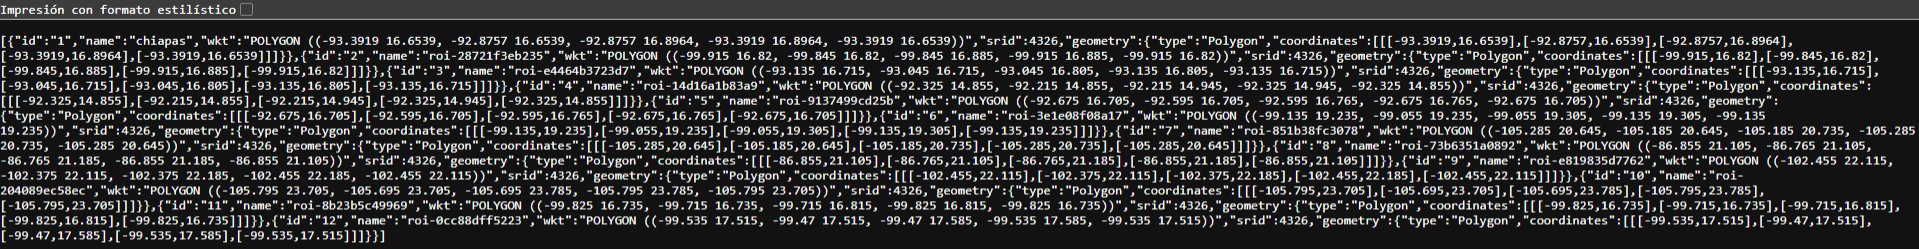
\includegraphics[width=0.84\textwidth]{fig/IMG_api_rest_contratos_json.png}
  \caption{Inspection of the TerraPulse AI REST API JSON contracts (\texttt{/api/scenes}, \texttt{/api/roi-jobs},
  and \texttt{/api/solar/simulations}), displaying HTTP headers, provenance fields (\texttt{code\_version},
  \texttt{warnings}), and structured GeoJSON/metric payloads.}
  \label{fig:img-api-rest-json}
\end{figure}

\section{Spatial Persistence in PostgreSQL/PostGIS and Docker Containerization}
\label{sec:arq-postgis-docker}

Relational and geospatial persistence is deployed via Docker Compose (\src{docker-compose.yml}) on the official
\texttt{postgis/postgis:16-3.4} image (PostgreSQL~16 with the PostGIS~3.4 spatial extension).

\subsection{Relational-Spatial Data Schema in PostGIS (\src{backend/scenes/models.py})}

The database stores four normalized entities that combine \texttt{EPSG:4326}-indexed geometries with
semi-structured \texttt{jsonb} columns for variable-length statistical series:

\begin{table}[htbp]
\centering
\small
\begin{tabular}{llp{4.1cm}p{6.5cm}}
\toprule
\textbf{SQL Table} & \textbf{Django Model} & \textbf{Uniqueness / Key Constraint} & \textbf{Spatial, JSONB Columns, and Integrity Rules} \\
\midrule
\texttt{scenes\_roi} & \texttt{ROI} & \texttt{id} (PK); reuses row if \texttt{geom} is spatially identical & \texttt{name} (\texttt{varchar}), \texttt{geom} (\texttt{PolygonField}, \texttt{SRID 4326}). Supports the fixed \texttt{chiapas} ROI and dynamic \texttt{roi-<12-hex>} ROIs. \\
\texttt{scenes\_scene} & \texttt{Scene} & Unique \texttt{name} (\texttt{granuleId}) & \texttt{product}, \texttt{track}, \texttt{frame}, \texttt{direction}, \texttt{polarizations} (\texttt{jsonb}), \texttt{frequency}, \texttt{band}, \texttt{epsg}, \texttt{crid}, \texttt{maturity} (nullable), \texttt{start\_time}, \texttt{footprint} (\texttt{PolygonField}, 2D \texttt{SRID 4326}). \\
\texttt{scenes\_sceneinspection} & \texttt{SceneInspection} & Unique per \texttt{(scene, roi, code\_version)} (migration \texttt{0002}) & \texttt{code\_version} (commit), \texttt{created\_utc}, \texttt{pct\_valid\_in\_roi}, \texttt{roi\_stats} (\texttt{jsonb}), \texttt{provenance} (\texttt{jsonb}), \texttt{warnings} (\texttt{jsonb}), \texttt{source\_dir}. \\
\texttt{scenes\_scenechart} & \texttt{SceneChart} & Unique per \texttt{(inspection, chart\_id)} & \texttt{chart\_id} (\texttt{varchar}), \texttt{format\_version} (\texttt{graficas-etapa1-1}), \texttt{source\_file}, \texttt{data} (\texttt{jsonb} holding the full \path{graficas.json} entry). \\
\bottomrule
\end{tabular}
\caption{Relational and spatial data model implemented in PostgreSQL 16 + PostGIS 3.4.}
\label{tab:esquema-postgis}
\end{table}

\subsection{Transactional Ingestion (\texttt{manage.py load\_explore}) and Resilient Backup}

The database \textbf{never opens \texttt{.h5} files or executes radiometric computations}: it consumes exclusively
the validated artifacts left by the pipeline (\path{metadatos.json} and \path{graficas.json}) through the
\texttt{python manage.py load\_explore --todas} command (or automatically upon job completion in
\src{roi\_views.py} via \texttt{copy\_to\_database}). The loader executes inside an atomic transaction
(\texttt{transaction.atomic()}) enforcing four scientific integrity rules:
\begin{enumerate}
  \item \textbf{Idempotency per code version:} reloading an inspection for the same
        $(\text{scene}, \text{ROI}, \texttt{code\_version})$ tuple updates that inspection in place and replaces
        its three charts; if the code commit changed, a new row is inserted into \texttt{scenes\_sceneinspection},
        preserving the history of previous versions for auditability.
  \item \textbf{Transactional rollback on inconsistency:} if \path{graficas.json} is missing, if the charts'
        \texttt{granuleId} disagrees with \path{metadatos.json}, if the two files originate from different commits,
        or if \texttt{version} differs from \texttt{graficas-etapa1-1}, the transaction rolls back without writing
        partial records.
  \item \textbf{Maturity level protection:} an ingestion generated in local mode (where the \texttt{.h5} file
        lacks the catalog's \texttt{dataMaturity} attribute and reports \texttt{null}) never overwrites a
        previously recorded maturity value (\texttt{PROVISIONAL} or \texttt{VALIDATED}) in \texttt{scenes\_scene}.
  \item \textbf{Container fault tolerance for web ROIs:} when an \texttt{/api/roi-jobs} run finishes,
        \src{pipeline/roi\_explore.py} first writes a durable disk copy to \path{data/graficas-roi/<id>/} and
        then attempts to synchronize it with PostGIS, recording the outcome in \path{copia.json}
        (\texttt{"base\_datos": "ok" | "parcial" | "no disponible"}). If Docker is stopped, the user still
        receives the map and charts in the web UI from disk, and runs can be ingested into PostGIS later via
        \texttt{python manage.py load\_explore --todas --dir data/graficas-roi/<id>}.
\end{enumerate}

\subsection{Docker Compose Orchestration, Volumes, and Port Coexistence}

\src{docker-compose.yml} defines the \texttt{db} service by decoupling credentials through the \path{.env} file
(never committed to Git) and mounting the named volume \texttt{pgdata} onto \path{/var/lib/postgresql/data}:

\begingroup\scriptsize
\begin{verbatim}
services:
  db:
    image: postgis/postgis:16-3.4
    restart: unless-stopped
    environment:
      POSTGRES_DB: ${POSTGRES_DB:-terrapulse}
      POSTGRES_USER: ${POSTGRES_USER:-terrapulse}
      POSTGRES_PASSWORD: ${POSTGRES_PASSWORD:?Set POSTGRES_PASSWORD in .env}
    ports:
      - "${POSTGRES_PORT:-5432}:5432"
    volumes:
      - pgdata:/var/lib/postgresql/data

volumes:
  pgdata:
\end{verbatim}
\endgroup

\begin{cuidado}
\warn{Resolving port \texttt{5432} conflicts with local PostgreSQL installations and password persistence in the
\texttt{pgdata} volume.}
On Windows or Linux workstations running a native PostgreSQL service (e.g., \texttt{postgresql-x64-18} listening
on \texttt{127.0.0.1:5432}), Django may accidentally connect to the host OS database engine instead of the PostGIS
container, raising \texttt{FATAL: password authentication failed for user "terrapulse"}. The configuration
architecture resolves this by setting \texttt{POSTGRES\_PORT=5433} in \path{.env}: Docker then publishes
\texttt{5433:5432} without stopping the developer's local database or losing data in the \texttt{pgdata} volume.
Furthermore, because the official PostgreSQL image evaluates \texttt{POSTGRES\_PASSWORD} only during the initial
\texttt{initdb} of an empty volume, any subsequent password change in \path{.env} requires updating the role via
\texttt{ALTER USER} in \texttt{psql} or recreating the volume with \texttt{docker compose down -v}.
\end{cuidado}

\begin{figure}[htbp]
  \centering
  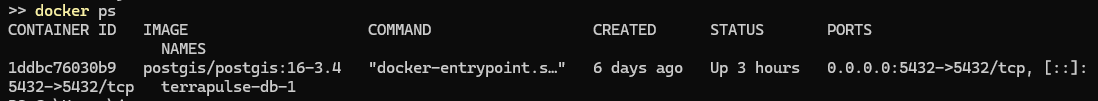
\includegraphics[width=0.84\textwidth]{fig/IMG_docker_postgis_esquema.png}
  \caption{PostgreSQL 16 + PostGIS 3.4 container running under Docker Compose along with a verification query over
  the spatial tables \texttt{scenes\_roi}, \texttt{scenes\_scene}, \texttt{scenes\_sceneinspection}, and
  \texttt{scenes\_scenechart}.}
  \label{fig:img-docker-postgis}
\end{figure}

\section{Scientific NASADEM Elevation Provider and Solar Simulator API}
\label{sec:arq-nasadem-solar}
\label{sec:solar-api-arch}

Alongside the NISAR radar pipeline, TerraPulse AI integrates a physical topography and incident direct solar
irradiance subsystem composed of the \src{pipeline/elevation/nasadem.py} provider, the \src{pipeline/solar/}
computational engine, and the \src{backend/solar/} HTTP services coupled to the interactive \textbf{Solar \&
Radiation Simulator} panel (\src{web/src/components/RightPanel.tsx} and \src{web/src/utils/solarHeatmap.ts}).

\subsection{The \texttt{NASADEMProvider} (\src{pipeline/elevation/nasadem.py})}

Unlike the browser's 3D terrain viewer (which consumes visual Terrarium tiles for fast WebGL rendering), all
backend scientific computations use the original \textbf{\texttt{NASADEM\_HGT} version \texttt{001}} granules
distributed by NASA Earthdata / LP DAAC. \texttt{NASADEMProvider} implements an acquisition protocol with strict
integrity and caching guarantees:

\begin{enumerate}
  \item \textbf{Exact geometric enumeration by positive-area intersection:} given a bounding box
        \texttt{(west, south, east, north)} or a GeoJSON \texttt{Polygon}/\texttt{MultiPolygon} in
        \texttt{EPSG:4326} within NASADEM's global coverage ($\text{lat} \in [-56^\circ, +60^\circ]$,
        $\text{lon} \in [-180^\circ, +180^\circ]$), \texttt{acquire\_roi} enumerates only those
        $1^\circ \times 1^\circ$ tiles (named by their southwest corner, e.g., \texttt{n16w094}) whose
        intersection with the ROI polygon has \textbf{strictly positive area}. If an ROI touches an exact integer
        degree boundary without occupying area in the adjacent tile, the neighbor tile is not downloaded.
  \item \textbf{Unambiguous NASA CMR lookup and non-interactive authentication:} for each missing tile, it queries
        the Common Metadata Repository (CMR) requiring a unique match for collection \texttt{NASADEM\_HGT} version
        \texttt{001} and \texttt{GranuleUR = NASADEM\_HGT\_<tile\_id>}. The session authenticates
        non-interactively via \texttt{earthaccess.login(strategy="environment", persist=False)} with a
        \texttt{strategy="netrc"} fallback, never persisting secrets to disk or leaking raw exception strings.
  \item \textbf{Structural HGT binary validation and staged publication:} each ZIP archive is downloaded into a
        temporary staging area inside the cache, rejecting symbolic links or path traversal outside the cache
        root. Before publication, the provider verifies that the ZIP contains exactly one \texttt{<tile\_id>.hgt}
        member with a valid CRC and exact byte length matching a $1\,\text{arc-second}$ grid ($3601 \times 3601$
        signed 16-bit big-endian integers, $25\,934\,402\,\text{bytes}$):
        \begin{equation}
          N_{\text{samples}} = 3601 \times 3601 = 12\,967\,201, \qquad
          \text{Size}_{\mathrm{HGT}} = 2 \times 3601^2 = 25\,934\,402\,\unit{bytes}.
          \label{eq:nasadem-hgt-size}
        \end{equation}
  \item \textbf{Offline local SHA-256 receipts:} once identity is confirmed against CMR, a local JSON receipt is
        written recording the \texttt{GranuleUR}, version, and SHA-256 cryptographic hash of the extracted HGT
        binary. On subsequent runs, if the ZIP and receipt SHA-256 match, the tile is returned as an immutable
        \texttt{NASADEMGranule(tile\_id, granule\_ur, short\_name, version, path)} tuple directly from disk
        without requiring network access or Earthdata credentials.
\end{enumerate}

\subsection{Physics and Mathematical Formulation of the Solar Simulator API (\texttt{/api/solar/simulations})}

The \texttt{POST /api/solar/simulations} endpoint computes over the NASADEM topographic grid the
\textbf{incident direct solar irradiance} $G_i(x,y)$ in $\unit{W/m^2}$ for a given local date/time
(\texttt{datetime\_local}), IANA time zone (\texttt{timezone}, e.g., \texttt{America/Mexico\_City}), intensity
percentage (\texttt{intensity\_percent} $\in [0, 100]$), and ambient temperature (\texttt{temperature\_c},
defaulting to $12\,^\circ\unit{C}$):

\begin{enumerate}
  \item \textbf{Standard-atmosphere barometric pressure and SPA solar position:} from the representative altitude
        $h_{\mathrm{rep}}$ (in meters above the EGM96 geoid) extracted from the ROI's NASADEM subset, if
        \texttt{pressure\_hpa} is not specified by the user, the engine computes local atmospheric pressure
        $P(h_{\mathrm{rep}})$ and evaluates the \emph{Solar Position Algorithm} (SPA, Reda \& Andreas) with
        atmospheric refraction correction to obtain apparent solar elevation $\alpha_s$, zenith angle
        $\theta_z = 90^\circ - \alpha_s$, and solar azimuth $\gamma_s$.
  \item \textbf{Clear-sky Direct Normal Irradiance (DNI) with Linke turbidity:} using the monthly Linke
        atmospheric turbidity climatology $T_L$ over the ROI (e.g., $T_L = 3.85$ in Chiapas in November), it
        computes clear-sky direct normal irradiance $\mathrm{DNI}_{\mathrm{cs}}$ (Ineichen \& Perez model) and
        applies the user-defined attenuation or cloud-transmittance factor
        ($p_{\mathrm{int}} = \texttt{intensity\_percent}/100$):
        \begin{equation}
          \mathrm{DNI}_{\mathrm{adj}} = \frac{\texttt{intensity\_percent}}{100} \cdot \mathrm{DNI}_{\mathrm{cs}}
          \quad [\unit{W/m^2}].
          \label{eq:solar-dni-adj}
        \end{equation}
  \item \textbf{Projection onto local topographic normal and incident irradiance $G_i(x,y)$:} the DEM is
        reprojected to the zone's metric UTM CRS (e.g., \texttt{EPSG:32615}, resolution $\approx 30.92\,\unit{m}$)
        and at each grid cell $(x,y)$ the topographic slope $\beta(x,y)$ and slope aspect $\gamma_t(x,y)$ are
        computed. The cosine of the solar incidence angle $\theta_i(x,y)$ between the unit sun-pointing vector
        $\hat{\mathbf{s}}(\theta_z, \gamma_s)$ and the outward slope normal $\hat{\mathbf{n}}(\beta, \gamma_t)$
        is given by:
        \begin{equation}
          \cos\theta_i(x,y) = \cos\theta_z\,\cos\beta(x,y)
          + \sin\theta_z\,\sin\beta(x,y)\,\cos\!\bigl(\gamma_s - \gamma_t(x,y)\bigr).
          \label{eq:solar-cos-incidencia}
        \end{equation}
        Whenever the Sun lies below the astronomical horizon ($\alpha_s \le 0^\circ$, \texttt{night: true}) or
        the slope's own inclination faces away from the Sun ($\cos\theta_i(x,y) \le 0$, topographic
        self-shadowing), incident direct irradiance vanishes:
        \begin{equation}
          G_i(x,y) =
          \begin{cases}
            0, & \text{if } \alpha_s \le 0^\circ \quad (\text{astronomical night}), \\[4pt]
            \mathrm{DNI}_{\mathrm{adj}} \cdot \max\!\bigl(0,\; \cos\theta_i(x,y)\bigr), & \text{if } \alpha_s > 0^\circ
            \quad [\unit{W/m^2}].
          \end{cases}
          \label{eq:solar-gi-incidente}
        \end{equation}
\end{enumerate}

\subsection{Solar Simulation JSON Contract, Point Sampling, and \emph{Inferno} LUT Inversion}

Execution is protected by a cross-platform inter-process file lock (\texttt{fcntl.flock} on Linux/POSIX and
\texttt{msvcrt.locking} on Windows in \src{backend/solar/services.py}; concurrent requests receive
\texttt{429 Too Many Requests}) and by strict operational budgets to prevent memory exhaustion (bounding box
$\le 0.25^\circ$ per axis, geodesic diagonal $\le 30\,\unit{km}$, at most 2 NASADEM tiles, and $\le 500\,000$
pixels; violations return \texttt{413 Payload Too Large}). Publication is atomic: the server writes the numerical
\texttt{float32} UTM GeoTIFF, the RGBA PNG preview rendered with the \emph{Inferno} palette in \texttt{EPSG:4326},
and the JSON manifest before returning \texttt{201 Created}:

\begingroup\scriptsize
\begin{verbatim}
POST /api/solar/simulations HTTP/1.1
Host: 127.0.0.1:8000
Content-Type: application/json

{
  "roi": {
    "type": "Polygon",
    "coordinates": [[
      [-93.56, 16.74], [-93.54, 16.74],
      [-93.54, 16.76], [-93.56, 16.76],
      [-93.56, 16.74]
    ]]
  },
  "datetime_local": "2026-11-15T12:00:00",
  "timezone": "America/Mexico_City",
  "intensity_percent": 50,
  "temperature_c": 12
}

HTTP/1.1 201 Created
Location: /api/solar/simulations/8e1a075f7712435bab9a0292d8eb36c0
Content-Type: application/json

{
  "id": "8e1a075f7712435bab9a0292d8eb36c0",
  "status": "ready",
  "units": "W/m2",
  "night": false,
  "position": {
    "datetime_utc": "2026-11-15T18:00:00+00:00",
    "apparent_elevation_deg": 54.63962031088027,
    "altitude_m": 782.1372680664062,
    "altitude_datum": "EGM96",
    "pressure_hpa": 922.7514462351598,
    "temperature_c": 12.0
  },
  "clear_sky": {
    "dni_clear_sky_w_m2": 885.3905049756529,
    "dni_adjusted_w_m2": 442.69525248782645,
    "intensity_percent": 50.0,
    "linke_turbidity": 3.85
  },
  "raster": {
    "crs": "EPSG:32615",
    "width": 72,
    "height": 74,
    "resolution_m": [30.92222222222222, 30.92222222222222],
    "units": "W/m2",
    "valid_pixels": 4968
  },
  "preview": {
    "crs": "EPSG:4326",
    "width": 74,
    "height": 73,
    "bounds_lonlat": [-93.56034941688789, 16.739547709324466, -93.53927810823552, 16.760334270562613],
    "palette": "inferno",
    "range_w_m2": [0.0, 442.69525248782645],
    "zero_range": false
  },
  "layers": {
    "incident": {
      "preview_url": "/api/solar/simulations/8e1a075f7712435bab9a0292d8eb36c0/preview/incident",
      "export_url": "/api/solar/simulations/8e1a075f7712435bab9a0292d8eb36c0/export/incident"
    }
  },
  "sample_url": "/api/solar/simulations/8e1a075f7712435bab9a0292d8eb36c0/sample"
}
\end{verbatim}
\endgroup

To query the exact numerical value at any geographic coordinate without interpolating or reading from the PNG,
\texttt{GET /api/solar/simulations/\{id\}/sample?lon=-93.55\&lat=16.75} projects $(\text{lon}, \text{lat})$ from
WGS84 into the GeoTIFF's UTM CRS (\texttt{EPSG:32615}) and returns the exact grid cell value:

\begingroup\scriptsize
\begin{verbatim}
GET /api/solar/simulations/8e1a075f7712435bab9a0292d8eb36c0/sample?lon=-93.55&lat=16.75 HTTP/1.1
Host: 127.0.0.1:8000
Accept: application/json

HTTP/1.1 200 OK
Content-Type: application/json

{
  "value_w_m2": 400.95941162109375,
  "status": "valid"
}
\end{verbatim}
\endgroup

\begin{ejemplo}[Client-side \emph{Inferno} LUT inversion and verification against \texttt{incident.tif}]
The PNG delivered by \texttt{preview/incident} is linearly normalized across the absolute interval
$[0, \mathrm{DNI}_{\mathrm{adj}}]$ using Matplotlib's 256-color \emph{Inferno} lookup table:
\begin{equation}
  u(x,y) = \operatorname{clip}\!\left(\frac{G_i(x,y)}{\mathrm{DNI}_{\mathrm{adj}}},\; 0,\; 1\right),
  \qquad
  k = \operatorname{round}(255 \cdot u(x,y)) \in \{0, 1, \ldots, 255\}.
  \label{eq:solar-lut-forward}
\end{equation}
When an ROI covers moderate relief (e.g., a $2$ to $5\,\unit{km}$ radius where nearly all slopes receive between
$398$ and $450\,\unit{W/m^2}$ out of $\mathrm{DNI}_{\mathrm{adj}} = 500\,\unit{W/m^2}$), all pixels fall into a
narrow yellow-orange band and geomorphological differences between north- and south-facing slopes are barely
distinguishable to the naked eye.

To provide instant contrast enhancement in the browser without re-fetching the TIFF from the server,
\src{web/src/utils/solarHeatmap.ts} builds the inverse lookup table of the 256 \emph{Inferno} RGB triplets and
recovers the estimated physical irradiance $\hat{G}_i(x,y)$ for every opaque pixel ($\alpha > 0$) by finding the
index $k^\star$ of minimum squared Euclidean distance in RGB color space:
\begin{equation}
  k^\star(x,y) = \arg\min_{k\in\{0,\ldots,255\}} \bigl\|\mathbf{c}_{\mathrm{PNG}}(x,y) - \mathbf{c}_{\mathrm{Inferno}}(k)\bigr\|_2^2,
  \qquad
  \hat{G}_i(x,y) = \frac{k^\star(x,y)}{255}\,\mathrm{DNI}_{\mathrm{adj}},
  \label{eq:solar-lut-inverse}
\end{equation}
whose quantization resolution is $\pm \mathrm{DNI}_{\mathrm{adj}} / 512 \approx \pm 1\,\unit{W/m^2}$. From the
recovered matrix $\hat{G}_i(x,y)$, the browser computes the dashboard summary statistics (minimum, maximum,
median, mean, and quantiles $p_2, p_{98}$) and allows toggling between two display modes:
\begin{itemize}
  \item \textbf{Absolute Mode ($[0, \mathrm{DNI}_{\mathrm{adj}}]$):} preserves the absolute physical scale for
        direct comparison across different times of day.
  \item \textbf{Contrast Mode ($[p_2, p_{98}]$):} dynamically rescales the \emph{Inferno} ramp between the 2nd
        and 98th percentiles of the active ROI, sharply revealing ravines and ridgelines.
\end{itemize}
In a real test over a $5\,\unit{km}$ radius in Chiapas ($324\times 326\,\text{px}$, $30\,\unit{m}$ NASADEM), the
quantiles recovered from the PNG in the browser ($p_2 = 294\,\unit{W/m^2}$, $\text{median} = 423\,\unit{W/m^2}$,
$p_{98} = 479\,\unit{W/m^2}$) agreed within $\le 1\,\unit{W/m^2}$ with the exact 32-bit floating-point values
measured on \path{incident.tif} ($293$, $423$, and $480\,\unit{W/m^2}$, verified in
\src{web/tests/solarHeatmap.test.mjs}).
\end{ejemplo}

\begin{atencion}
The solar simulator computes exclusively \textbf{clear-sky direct solar irradiance incident on terrain, modulated
by local slope geometry and the user's intensity factor}. It is not an in-situ pyranometer measurement, does not
include anisotropic diffuse sky radiation or terrain-reflected irradiance (albedo), and does not model thermal
balance, absorption, or land surface temperature. This explicit physical scope boundary is displayed both in the
API documentation and in the user interface warnings.
\end{atencion}

\begin{figure}[htbp]
  \centering
  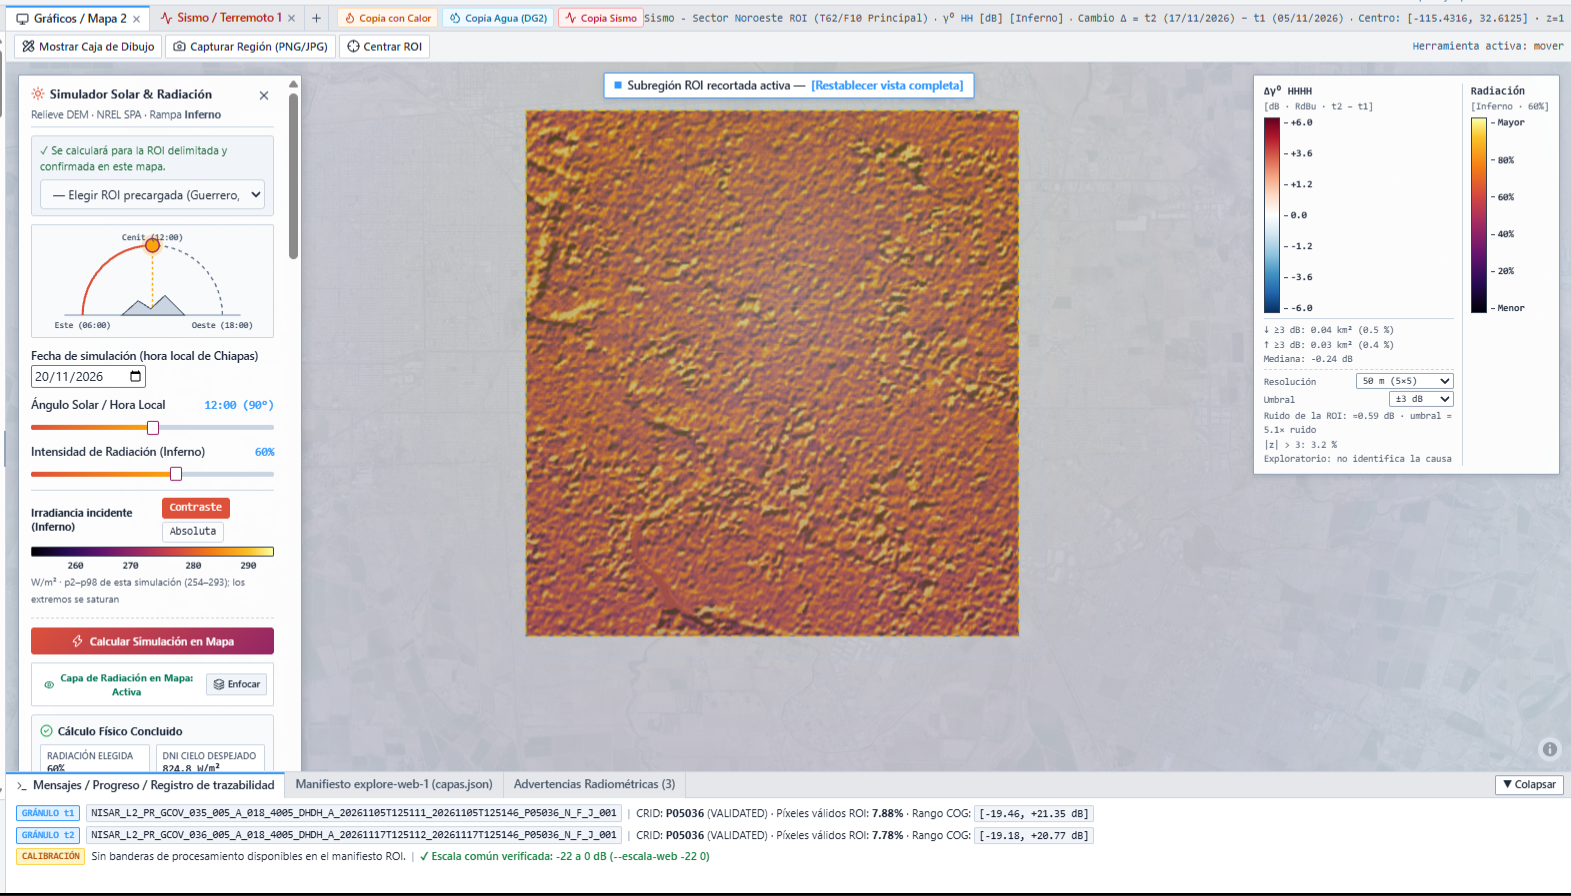
\includegraphics[width=0.84\textwidth]{fig/IMG_simulador_solar_heatmap_ui.png}
  \caption{Interactive \textbf{Solar \& Radiation Simulator} panel in the TerraPulse AI web interface, showing
  the incident direct irradiance heatmap ($G_i$ in $\unit{W/m^2}$) over NASADEM terrain with the \emph{Inferno}
  palette, the \textbf{Contrast ($p_2\text{--}p_{98}$)} / \textbf{Absolute ($0\text{--}\mathrm{DNI}$)} scale
  toggle, and the solar telemetry dashboard (SPA apparent elevation, clear-sky and adjusted DNI, median, and
  irradiance range across the ROI).}
  \label{fig:img-simulador-solar-ui}
\end{figure}

\end{document}